\PassOptionsToPackage{unicode=true}{hyperref} % options for packages loaded elsewhere
\PassOptionsToPackage{hyphens}{url}
%
\documentclass[
  12pt,
  twoside,
  banjiao]{ctexbook}
\usepackage{lmodern}
\usepackage{amssymb,amsmath}
\usepackage{ifxetex,ifluatex}

\usepackage{unicode-math}
\defaultfontfeatures{Scale=MatchLowercase}
\defaultfontfeatures[\rmfamily]{Ligatures=TeX,Scale=1}

% use upquote if available, for straight quotes in verbatim environments
\IfFileExists{upquote.sty}{\usepackage{upquote}}{}
\IfFileExists{microtype.sty}{% use microtype if available
  \usepackage[]{microtype}
  \UseMicrotypeSet[protrusion]{basicmath} % disable protrusion for tt fonts
}{}

\usepackage{xcolor}
\usepackage{subfig}
\usepackage{xurl} % add URL line breaks if available
\usepackage{bookmark}
\usepackage[version=4]{mhchem}
\usepackage{hyperref}
\usepackage{float}
%\usepackage{placeins}
\usepackage[section]{placeins}
\makeatletter
\AtBeginDocument{%
  \expandafter\renewcommand\expandafter\subsection\expandafter{%
    \expandafter\@fb@secFB\subsection
  }%
}
\makeatother
\hypersetup{
  pdftitle={临床营养学},
  pdfauthor={github},
  pdfborder={0 0 0},
  breaklinks=true,
  bookmarksdepth=5}
\urlstyle{same}  % don't use monospace font for urls
\usepackage{longtable,booktabs}
% Allow footnotes in longtable head/foot
\IfFileExists{footnotehyper.sty}{\usepackage{footnotehyper}}{\usepackage{footnote}}
\makesavenoteenv{longtable}
\usepackage{graphicx,grffile}
\makeatletter
\def\maxwidth{\ifdim\Gin@nat@width>\linewidth\linewidth\else\Gin@nat@width\fi}
\def\maxheight{\ifdim\Gin@nat@height>\textheight\textheight\else\Gin@nat@height\fi}
\makeatother
% Scale images if necessary, so that they will not overflow the page
% margins by default, and it is still possible to overwrite the defaults
% using explicit options in \includegraphics[width, height, ...]{}
\setkeys{Gin}{width=\maxwidth,height=\maxheight,keepaspectratio}

\setlength{\emergencystretch}{3em}  % prevent overfull lines
% Redefines (sub)paragraphs to behave more like sections
\ifx\paragraph\undefined\else
  \let\oldparagraph\paragraph
  \renewcommand{\paragraph}[1]{\oldparagraph{#1}\mbox{}}
\fi
\ifx\subparagraph\undefined\else
  \let\oldsubparagraph\subparagraph
  \renewcommand{\subparagraph}[1]{\oldsubparagraph{#1}\mbox{}}
\fi

% set default figure placement to htbp
\makeatletter
\def\fps@figure{htbp}
\makeatother


\setcounter{secnumdepth}{5}
\usepackage{framed}
\usepackage{multirow}
\usepackage{ctex}
\usepackage{rotating}
\usepackage{tablefootnote}
\usepackage{caption}

\setCJKmainfont{思源宋体}
\setCJKfallbackfamilyfont{\CJKrmdefault}{宋体}
\setmainfont{思源宋体}
\usepackage[a4paper,top=1in, bottom=1in, left=0.8in, right=0.8in]{geometry}
\setlength{\parindent}{2em}
\setlength{\parskip}{0em}

%\newfontfamily\apostrophefont[Ligatures=TeX,Color=FF0000]{Liberation Serif}
\newfontfamily\apostrophefont[Ligatures=TeX]{Liberation Serif}
\XeTeXinterchartokenstate=1
\newXeTeXintercharclass \apostrophe

% Assign the new class to all Latin capital letters
\makeatletter
\@tempcnta=`'
\loop\unless\ifnum\@tempcnta>`'
  \XeTeXcharclass \@tempcnta \apostrophe
  \advance \@tempcnta by 1
\repeat
\makeatother

% Setup font change
\XeTeXinterchartoks 0 \apostrophe   = {\begingroup\apostrophefont}
\XeTeXinterchartoks \apostrophe 0   = {\endgroup}
\XeTeXinterchartoks 4095 \apostrophe = {\begingroup\apostrophefont}
\XeTeXinterchartoks \apostrophe 4095 = {\endgroup}

\renewcommand {\thetable} {\arabic{chapter}-\arabic{section}-\arabic{table}}
\renewcommand {\thefigure} {\arabic{chapter}-\arabic{section}-\arabic{figure}}
\newcommand\subsectiontitleformat[1]{\noindent 【#1】}
\usepackage{chngcntr}
\counterwithout{subsection}{chapter}
\counterwithout{subsection}{section}
\counterwithin{figure}{section}

\ctexset {
  section = {
    name
    = {第,节},
    number = \chinese{section},
  },
  subsection = {
    name 
    = {,、},
    number = \chinese{subsection}
  }
}


\title{临床营养学}
\author{github \\ 项目主页:\url{https://github.com/scienceasdf/medical-books}\\ 新书下载:\url{https://github.com/scienceasdf/medical-books/releases/latest}}


\begin{document}
\maketitle
\frontmatter
{
\setcounter{tocdepth}{1}
\tableofcontents
\addcontentsline{toc}{chapter}{目录}
}
\newpage

\mainmatter
\chapter{多器官功能障碍综合征和多器官功能衰竭}

\section{前沿学术综述}

多器官功能障碍综合征(multiple organ dysfunction
syndrome,MODS)是指机体遭受到严重感染、创伤、烧伤等严重打击后,两个或两个以上的器官同时或序贯性功能障碍。大量临床研究显示,器官障碍程度越重、器官障碍数目越多、患者病死率越高。若MODS发展为多器官功能衰竭(multiple
organ
failure,MOF),病死率可高达60%~94%,是严重感染、创伤和大手术后最常见的病死原因
\protect\hyperlink{text00007.htmlux5cux23ch1-6}{\textsuperscript{{[}1{]}}}
。急性器官障碍的数目和严重程度,明显影响患者的生活质量和病死率,多器官功能衰竭及MODS是当前重症医学所面临的最大挑战
\protect\hyperlink{text00007.htmlux5cux23ch2-6}{\textsuperscript{{[}2{]}}}
。

MODS的发病机制非常复杂。以往认为MODS是感染、创伤、烧伤等严重机体损伤难以遏制的直接后果。近20年的研究涉及到了MODS的病理生理学、病理学、免疫学、分子生物学以及分子流行病学,对MODS的认识逐步深刻。目前认为,MODS不仅与感染、创伤等直接损伤有关,在某种程度上,MODS与机体自身对感染、创伤的免疫炎症反应具有更为本质性的联系。也就是说,MODS的最大威胁来自失控的炎症反应
\protect\hyperlink{text00007.htmlux5cux23ch2-6}{\textsuperscript{{[}2{]}}}
。对机体炎症反应的深刻认识有利于早期认识MODS的病理生理紊乱,并使早期积极干预成为可能
\protect\hyperlink{text00007.htmlux5cux23ch3-6}{\textsuperscript{{[}3{]}}}
。MODS的发病机制提出了不少学说,但归纳起来主要包括炎症反应学说、自由基学说和肠道动力学说
\protect\hyperlink{text00007.htmlux5cux23ch2-6}{\textsuperscript{{[}2{]}}}
\textsuperscript{,}
\protect\hyperlink{text00007.htmlux5cux23ch4-6}{\textsuperscript{{[}4{]}}}
\textsuperscript{~}
\protect\hyperlink{text00007.htmlux5cux23ch6-6}{\textsuperscript{{[}6{]}}}
。炎症反应学说是MODS发病机制的基石。

根据MODS器官功能障碍发生的主要原因以及全身炎症反应综合征(systemic
inflammatory response
syndrome,SIRS)在器官功能损伤中的地位,可将MODS分为原发性MODS和继发性MODS。原发性MODS是指某种明确的损伤直接引起器官功能障碍,即器官功能障碍由损伤本身引起,在损伤早期出现,如严重创伤后,直接肺挫伤导致急性呼吸衰竭,横纹肌溶解导致肾脏功能衰竭,大量出血补液导致凝血功能异常等。在原发性MODS的发病和演进过程中,全身炎症反应综合征在器官功能障碍发生中所占比重较低。继发性MODS并非是损伤的直接后果,而与全身炎症反应综合征引起的自身性破坏关系密切,异常的炎症反应继发性造成远隔器官发生功能障碍。所以,继发性MODS与原发损伤之间存在一定的间歇期,易合并感染。在继发性MODS中,全身炎症反应综合征是器官功能损害的基础,全身性感染和器官功能损害是SIRS的后继过程。全身炎症反应综合征---全身性感染---MODS就构成一个连续体,继发性MODS是该连续体造成的严重后果
\protect\hyperlink{text00007.htmlux5cux23ch4-6}{\textsuperscript{{[}4{]}}}
\textsuperscript{,}
\protect\hyperlink{text00007.htmlux5cux23ch5-6}{\textsuperscript{{[}5{]}}}
。

近年的研究证实,免疫功能障碍不仅是MODS的重要组成部分,同时在MODS发生发展中发挥关键的作用。MODS免疫功能障碍包括机体过度或失控炎症反应和免疫功能麻痹的动态过程。免疫功能障碍发病机制复杂,多种因素交互促成。严重感染、创伤后机体免疫功能发生紊乱,既可能表现为亢进,也可能低下,且往往表现为早期炎症反应亢进,后期发生免疫功能抑制
\protect\hyperlink{text00007.htmlux5cux23ch6-6}{\textsuperscript{{[}6{]}}}
。

MODS涉及面广,临床表现复杂,但MODS具有以下显著特征:①发生功能障碍的器官往往是直接损伤器官的远隔器官;②从原发损伤到发生器官功能障碍在时间上有一定的间隔;③高排低阻的高动力状态是循环系统的特征;④高氧输送和氧利用障碍及内脏器官缺血缺氧,使氧供需矛盾尖锐;⑤持续高代谢状态和能源利用障碍。

所有MODS患者均应进入重症医学科治疗。尽管MODS的病因复杂、涉及的器官和系统多,治疗中往往面临很多矛盾,但MODS的治疗应遵循以下原则:

(1)积极治疗原发病 控制原发疾病是MODS治疗的关键,应重视原发疾病的处理。

(2)改善氧代谢,纠正组织缺氧 氧代谢障碍是MODS的特征之一,纠正组织缺氧是MODS重要的治疗目标。改善氧代谢障碍、纠正组织缺氧的主要手段包括增加全身氧输送、降低全身氧需、改善组织细胞利用氧的能力等。

(3)代谢支持与调理 MODS使患者处于高度应激状态,导致机体出现以高分解代谢为特征的代谢紊乱。器官及组织细胞的功能维护和组织修复有赖于细胞得到适当的营养底物,机体高分解代谢和外源性营养利用障碍,可导致或进一步加重器官功能障碍。因此,MODS时,代谢支持和调理的目标应当是减轻营养底物不足,防止细胞代谢紊乱,减少器官功能障碍的产生,促进组织修复。

(4)免疫调节治疗 免疫功能障碍、炎症反应失控是导致MODS的根本原因,免疫调控治疗、抑制全身炎症反应有可能阻断MODS的发展,最终可能降低MODS病死率。免疫调节治疗实际上就是MODS病因治疗的重要方向。

\section{临床问题}

\subsubsection{为什么要提出多器官功能障碍综合征的概念?}

多器官功能障碍综合征(MODS)的终末阶段是多器官功能衰竭。以MODS的概念代替多器官功能衰竭,反映了人们对多器官功能衰竭更为深入的认识和了解,将MODS定义为一个包括早期病理生理改变到终末期器官功能衰竭的连续的完整的病理生理过程,确立了动态和开放的MODS概念,为MODS的早期认识、早期诊断以及早期干预奠定了基础,具有重要的临床意义。

MODS概念的提出是认识进步的结果,但确定较为合理的MODS定义仍然困难。为了避免割裂MODS整个病理生理过程,美国胸科医师学会和美国危重病医学会提出了一个较为模糊的MODS定义,即各种疾病导致多个器官不能维持自身功能,从而影响全身内环境稳定性的状态。MODS表述的器官功能障碍可以是相对的,也可以是绝对的,而且器官功能障碍是动态的、连续的变化过程,对器官功能的动态观察必将有助于MODS的早期诊断和治疗。

\subsubsection{全身炎症反应综合征有何临床意义?}

1991年在芝加哥召开的美国胸科医师学会和危重病医学会联席会议,将感染或创伤引起的持续全身炎症反应失控的临床表现命名为全身炎症反应综合征,并制定了相应的诊断标准(表\ref{tab1-1})。全身炎症反应综合征可由感染因素引起,若进行性加重可导致全身性感染(systemic
infection或sepsis)、严重感染(severe
sepsis)、感染性休克,甚至多器官功能障碍综合征(MODS)。全身炎症反应综合征也可由创伤、烧伤、急性重症胰腺炎等非感染因素引起,进行性加重亦可引起MODS。全身炎症反应综合征是感染或非感染因素导致机体过度炎症反应的共同特征,MODS是全身炎症反应综合征进行性加重的最终后果。因此,就本质而言,全身炎症反应综合征是导致MODS的共同途径。

\begin{table}[htbp]
\centering
\caption{全身炎症反应综合征的诊断标准(符合下列两项或两项以上)}
\label{tab1-1}

\includegraphics[width=\textwidth,height=\textheight,keepaspectratio]{./images/Image00001.jpg}
\end{table}

尽管全身炎症反应综合征概念的提出是MODS认识上的重大进步,但全身炎症反应综合征的诊断标准本身存在许多不足,特别是把它作为一个综合征或疾病时,不能停留在诊断水平上,应积极寻找导致全身炎症反应综合征的致病因素。当然,我们也不能因为全身炎症反应综合征诊断标准存在问题而否认全身炎症反应综合征的重要意义。

\subsubsection{怎么认识多器官功能障碍综合征的病理生理机制?}

正常情况下,感染和组织创伤时,局部炎症反应对细菌清除和损伤组织修复都是必要的,具有保护性作用。当炎症反应异常放大或失控时,炎症反应对机体的作用从保护性转变为损害性,导致自身组织细胞死亡和器官衰竭。无论是感染性疾病(如严重感染、重症肺炎、急性重症胰腺炎后期),还是非感染性疾病(如创伤、烧伤、休克、急性胰腺炎早期等)均可能导致多器官功能障碍综合征(MODS)。可见,任何能够导致机体免疫炎症反应紊乱的疾病均可引起MODS。从本质上来看,MODS是机体炎症反应失控的结果。

感染、创伤是机体炎症反应的促发因素,而机体炎症反应的失控,最终导致机体自身性破坏,是MODS的根本原因。炎症细胞激活和炎症介质异常释放、组织缺氧和自由基、肠道屏障功能破坏和细菌和(或)毒素移位均是机体炎症反应失控的表现,构成了MODS炎症反应失控的3个互相重叠的发病机制学说------炎症反应学说、自由基学说和肠道动力学说(图\ref{fig1-1})。

\begin{figure}[!htbp]
 \centering
 
\includegraphics{./images/Image00002.jpg}
 \captionsetup{justification=centering}
 \caption{多器官功能障碍综合征的发病机制}
 \label{fig1-1}
  \end{figure} 

(1)炎症反应学说 炎症反应学说是MODS发病机制的基石。研究表明,感染或创伤引起的毒素释放和组织损伤并不是导致器官功能衰竭的直接原因,细菌和(或)毒素和组织损伤所诱发的全身炎症反应是导致器官功能衰竭的根本原因。

(2)缺血再灌注和自由基学说 缺血再灌注和自由基也是导致MODS的重要机制之一。MODS的自由基学说主要包括3方面:①氧输送不足导致组织细胞直接的缺血缺氧性损害;②缺血再灌注促发自由基大量释放;③白细胞与内皮细胞的互相作用,导致组织和器官损伤,最终发生MODS。从根本上来看,自由基学说也是炎症反应学说的重要组成部分。

(3)肠道动力学说 肠道动力学说的概念最早是由Meakins和Marshall提出的。肠道是机体最大的细菌和毒素库,肠道有可能是MODS患者菌血症的来源。另外,MODS患者菌血症的细菌往往与肠道菌群一致。因此,Meakins和Marshall提出肠道可能是MODS发生发展的动力器官(gut
motor)。在感染、创伤或休克时,即使没有细菌的移位,肠道内毒素的移位也将激活肠道及其相关的免疫炎症细胞,导致大量炎症介质的释放,参与MODS的发病。因此,肠道是炎症细胞激活、炎症介质释放的重要场地之一,也是炎症反应失控的策源地之一。从这一点来看,肠道动力学说实际上是炎症反应学说的一部分。

\subsubsection{全身炎症反应失衡怎样导致多器官功能障碍综合征的发生?}

基于全身炎症反应综合征是导致多器官功能障碍综合征(MODS)的根本原因这一认识,抑制全身炎症反应综合征有可能阻断炎症反应发展,最终可能降低MODS的病死率。20世纪90年代初期,大量的动物实验研究显示,抑制炎症介质能够明显降低感染或内毒素血症动物的病死率,这为临床MODS的救治带来希望。令人失望的是,内毒素单抗、肿瘤坏死因子α单抗等炎症介质拮抗剂在临床试验中相继失败,甚至个别研究报道增加病死率。由此迫使人们深入研究,并重新认识全身炎症反应综合征在MODS中的作用。

首先,引起注意的是机体受细菌毒素、损伤打击后,出现一过性细胞免疫功能降低,使机体对感染易感;其次,机体受细菌毒素、损伤刺激后,不仅释放炎症介质引起全身炎症反应综合征,同时大量释放内源性抗炎介质,后者可能是导致机体免疫功能损害的主要原因;第三,临床上盲目使用炎症介质拮抗剂,可能使免疫功能损伤加重,或许这就是炎症介质拮抗剂临床试验失败的主要原因。鉴于上述认识,1996年Bone针对感染或创伤时,导致机体免疫功能降低的内源性抗炎反应,提出了代偿性抗炎反应综合征(compensatory
anti-inflammatory response
syndrome,CARS)的概念。代偿性抗炎反应综合征作为全身炎症反应综合征的对立面,两者常常是不平衡的。如保持平衡,则内环境稳定得以维持,不会引起器官功能损伤。一旦全身炎症反应综合征和代偿性抗炎反应综合征失衡,将引起内环境失去稳定性,导致组织器官损伤,发生MODS
\protect\hyperlink{text00007.htmlux5cux23ch7-6}{\textsuperscript{{[}7{]}}}
\textsuperscript{,}
\protect\hyperlink{text00007.htmlux5cux23ch8-6}{\textsuperscript{{[}8{]}}}
。

如果把全身炎症反应综合征和代偿性抗炎反应综合征看作机体炎症反应天平的两端,则代偿性抗炎反应综合征作为天平的另一端,对全身炎症反应综合征发生、发展所起的关键性作用是不言而喻的。代偿性抗炎反应综合征的发生主要与抗炎性介质合成、抗炎性内分泌激素及炎症细胞凋亡等因素有关。

就其本质而言,MODS是全身炎症反应综合征和代偿性抗炎反应综合征免疫失衡的严重后果。全身炎症反应综合征和代偿性抗炎反应综合征失衡导致MODS的发展过程可分为3个阶段:①局限性炎症反应阶段,局部损伤或感染导致炎症介质在组织局部释放,诱导炎症细胞向局部聚集,促进病原微生物清除和组织修复,对机体发挥保护作用;②有限全身炎症反应阶段,少量炎症介质进入循环诱发全身炎症反应综合征,诱导巨噬细胞和血小板向局部聚集,同时,由于内源性抗炎介质释放增加导致代偿性抗炎反应综合征,使全身炎症反应综合征与代偿性抗炎反应综合征处于平衡状态,炎症反应仍属生理性,目的在于增强局部防御作用;③全身炎症反应综合征和代偿性抗炎反应综合征失衡阶段,表现为两个极端,一是大量炎症介质释放入循环,刺激炎症介质瀑布样释放,而内源性抗炎介质又不足以抵消其作用,导致全身炎症反应综合征;另一个极端是内源性抗炎介质释放过多而导致代偿性抗炎反应综合征。全身炎症反应综合征和代偿性抗炎反应综合征失衡的后果是炎症反应失控,使其由保护性作用转变为自身破坏性作用,不但损伤局部组织,同时打击远隔器官,导致MODS。

认识的进步,必然预示着在治疗上取得突破。恢复全身炎症反应综合征和代偿性抗炎反应综合征的动态平衡可能是MODS治疗的关键。

\subsubsection{多器官功能障碍综合征的二次打击学说有何临床意义?}

多器官功能障碍综合征(MODS)往往是多元性和序贯性损伤的结果,而不是单一打击的结果。1985年Dietch提出MODS的二次打击学说,将创伤、感染、烧伤、休克等早期直接损伤作为第一次打击,第一次打击所造成的组织器官损伤是轻微的,虽不足以引起明显的临床症状,但最为重要的是,早期损伤激活了机体免疫系统,尽管炎症反应的程度较轻,但炎症细胞已经被动员起来,处于预激活状态。此后,如病情稳定,则炎症反应逐渐缓解,损伤组织得以修复;如病情进展恶化或继发感染、休克等情况,则构成第二次或第三次打击。第二次打击使已处于预激活状态的机体免疫系统爆发性激活,大量炎症细胞活化、炎症介质释放,结果炎症反应失控,导致组织器官的致命性损害。第二次打击强度本身可能不如第一次打击,但导致炎症反应的爆发性激活,往往是致命性的(图\ref{fig1-2})。

\begin{figure}[!htbp]
 \centering
 
\includegraphics{./images/Image00003.jpg}
 \captionsetup{justification=centering}
 \caption{多器官功能障碍综合征的二次打击学说}
 \label{fig1-2}
  \end{figure} 

当第一打击强度足够大时,可直接强烈激活机体炎症反应,导致MODS,属于原发性MODS。但大多数患者MODS是多元性和序贯性损伤的结果,并不是单一打击的结果,这类MODS属于继发性MODS。常见的第二次打击包括继发性感染、休克、缺氧、缺血、创伤、手术等。对于多发性创伤的患者,如创伤严重,则直接可导致MODS,但多数患者经早期清创处理后基本稳定,而创伤早期发生的低血压导致各器官发生不同程度的缺血再灌注损伤及巨噬细胞、中性粒细胞激活,使患者出现发热、白细胞升高等炎症反应表现。创伤后3~7天,继发性感染或休克,使已处于预激活或激活状态的炎症细胞发生爆发性激活,结果使炎症反应失控,导致自身组织器官的损害,最终发展为MODS。

危重患者的病情往往是复杂的,机体遭受打击次数可能是两次,也可能是多次。多次反复打击将使机体炎症反应放大和失控更易发生,使患者更易发生MODS。另外,不仅机体免疫系统参与多次打击导致MODS的病理生理过程,凝血、纤溶、补体、激肽等多个系统均参与或累及。

MODS二次打击学说的提出,进一步强调了感染、创伤的后期处理。后期处理不当,其后果比早期损伤的结果更为严重,更具危害性。

\subsubsection{多器官功能障碍综合征有哪些临床特征?}

尽管多器官功能障碍综合征(MODS)的临床表现很复杂,但在很大程度上取决于器官受累的范围及损伤是由一次打击还是由多次打击所致。MODS临床表现的个体差异很大,一般情况下,MODS病程为14~21天,并经历4个阶段,包括休克、复苏、高分解代谢状态和器官衰竭阶段。每个阶段都有其典型的临床特征(表\ref{tab1-2}),且发展速度极快,患者可能死于MODS的任一阶段。

\begin{table}[htbp]
\centering
\caption{MODS的临床分期和特征}
\label{tab1-2}
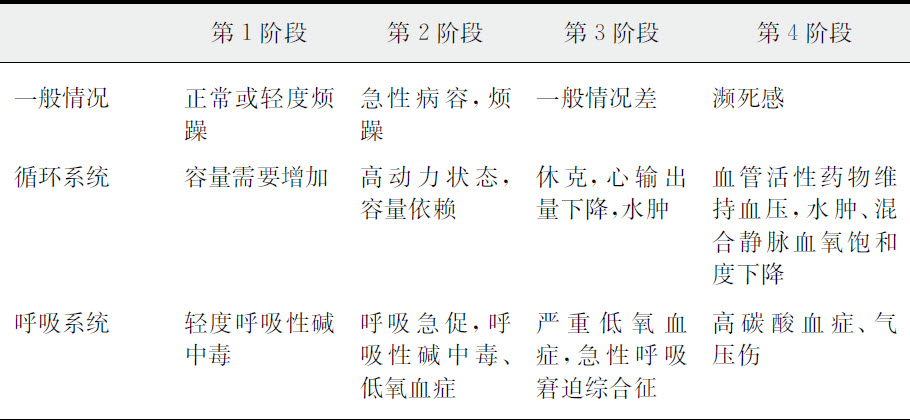
\includegraphics[width=\textwidth,height=\textheight,keepaspectratio]{./images/Image00004.jpg}
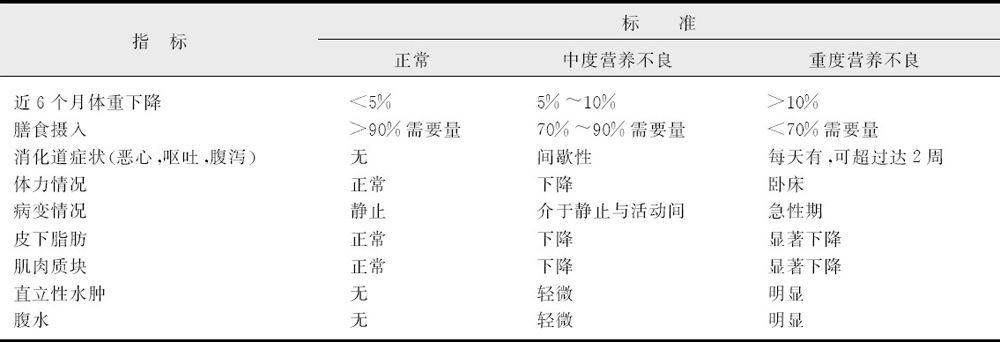
\includegraphics[width=\textwidth,height=\textheight,keepaspectratio]{./images/Image00005.jpg}
\end{table}



\subsubsection{不同多器官功能障碍综合征诊断标准有何差异?}

1980年Fry提出第一个多器官功能衰竭诊断标准。在此之前,循环、呼吸、肾脏和肝脏等器官已经具有单一器官衰竭的判断或诊断标准。应激性上消化道出血被认为是胃肠道功能衰竭。然而,血液、代谢和神经系统的衰竭或功能紊乱就缺乏明确的诊断方法。DIC显然是血液系统的功能紊乱,DIC诊断中除了出血等临床表现外,还需有血浆纤维蛋白降解产物水平升高。但血浆纤维蛋白降解产物浓度升高缺乏特异性,严重创伤或手术患者也可升高,使血液系统功能衰竭的诊断缺乏客观性。代谢紊乱是重症患者应激的结果,如果能够对代谢过程进行复杂的监测,则所有重症患者可能都存在所谓的“代谢障碍”,对代谢障碍的诊断缺乏可行性。神经系统功能障碍在重症患者中也很常见,但准确定量评价非常困难。另外,严重感染导致内脏器官严重损害时,往往血压和心输出量是正常或偏高的,直到出现休克或临终期,心血管系统才表现出功能衰竭。因此,Fry在提出多器官功能衰竭诊断标准时,仅包含了呼吸、肝脏、肾脏和胃肠道系统(表\ref{tab1-3})。

\begin{table}[htbp]
\centering
\caption{多器官功能衰竭诊断标准(Fry,1980年)}
\label{tab1-3}
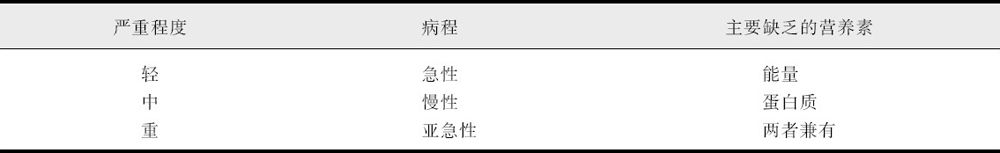
\includegraphics[width=\textwidth,height=\textheight,keepaspectratio]{./images/Image00006.jpg}
\end{table}

尽管Fry的多器官功能衰竭诊断标准是目前被公认的、应用最普遍的诊断标准,仍然存在很多问题:①该标准未包括神经系统、循环系统、血液系统等常见的器官功能衰竭;②以终末期的功能衰竭为诊断标准,不利于早期诊断和治疗;③难以反映多器官功能衰竭动态连续变化的病理生理过程;④呼吸功能衰竭的诊断过于严格,容易漏诊。

针对Fry诊断标准存在的问题,我们于1997年提出了修正的Fry-多器官功能障碍综合征(MODS)诊断标准(表\ref{tab1-4}),该标准结合国际常用的诊断标准,几乎包括了所有可能累及的器官或系统。当然,该标准未能包括MODS的整个病理生理过程,但避免了繁琐的程度评分,较为简捷,增加了临床实用性。

\begin{table}[htbp]
\centering
\caption{MODS诊断标准}
\label{tab1-4}
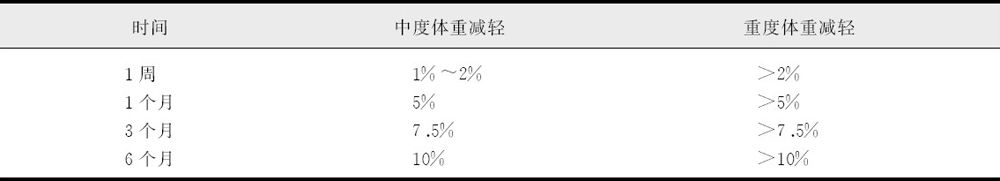
\includegraphics[width=\textwidth,height=\textheight,keepaspectratio]{./images/Image00007.jpg}
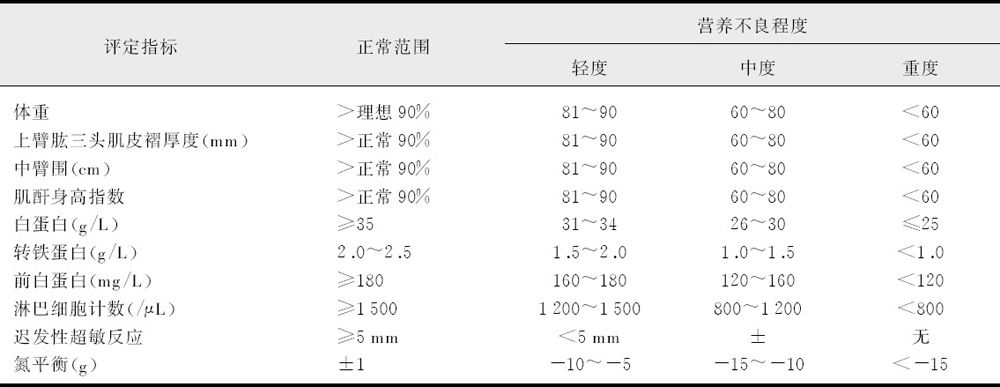
\includegraphics[width=\textwidth,height=\textheight,keepaspectratio]{./images/Image00008.jpg}
\end{table}

\subsubsection{哪些因素导致多器官功能障碍综合征的病死率增加?}

多器官功能障碍综合征(MODS)患者病死率高,认识病死危险因素,有助于早期确立MODS治疗对策。Knaus等学者对MODS的病死危险因素做了大规模的临床调查,概括了MODS病死的相关危险因素(表\ref{tab1-5})。\footnote{* APACHE:急性生理和慢性健康状况评分。}

\begin{table}[htbp]
\centering
\caption{MODS的病死危险因素}
\label{tab1-5}
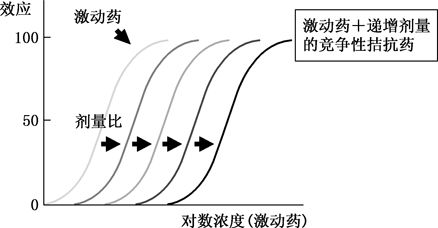
\includegraphics[width=\textwidth,height=\textheight,keepaspectratio]{./images/Image00009.jpg}
\end{table}

我国的研究也显示,免疫功能低下、转入ICU时的急性生理和既往健康评分(APACHE)Ⅱ评分、非手术、感染性休克及器官衰竭数目等因素与MODS患者死亡的关系显著。创伤、感染等MODS的病因、全身炎症反应综合征程度等因素与患者病死率无明显关系。

循环功能衰竭,即感染性休克为MODS最常见的直接病死原因;其次为中枢神经系统功能衰竭和心功能衰竭等,进一步提示在MODS治疗中,应特别注意纠正循环衰竭,并针对病因采取有效治疗措施,不应掉以轻心。

总之,MODS病死率依然很高,针对MODS病死危险因素进行积极处理和干预,可能是降低MODS病死率的关键。

\subsubsection{多器官功能障碍综合征时免疫功能障碍的基本概念是什么?}

免疫功能障碍不仅是多器官功能障碍综合征(MODS)的重要组成部分,同时在MODS发生发展中发挥关键的作用。MODS免疫功能障碍包括机体过度或失控炎症反应和免疫功能麻痹的动态过程。炎症反应本质上属于免疫反应的范畴,失控的炎症反应是MODS发生发展的根本机制,严重的炎症反应或细胞因子风暴可迅速引起微循环衰竭和感染性休克,继而发生DIC、呼吸衰竭和肝肾等器官功能障碍。免疫功能抑制可能与免疫效应细胞减少或功能抑制、机体呈调节T细胞或Th2极化和抗炎介质释放增多等因素有关。

临床免疫功能障碍可表现为多器官功能障碍,可于数小时、数天或数周发病,病程也长短不一。如爆发型流脑、中毒性休克综合征及严重猪链球菌Ⅱ型感染等严重炎症反应常在很短的时间内迅速发生休克、呼吸衰竭、肾衰竭和DIC等。免疫功能抑制患者常表现为原发感染难以痊愈,潜在感染的复发,或出现新的继发性感染。目前准确定量评价机体炎症反应水平和免疫功能紊乱性质、程度仍存在困难,还缺乏准确的临床判断指标和诊断方法。通过仔细的临床观察和密切的实验室检测,早期诊断器官功能损害或衰竭,并给予强化的器官功能支持治疗,能够避免部分患者死于继发性器官功能衰竭。

尽管MODS中免疫功能衰竭日益受到重视,然而由于其功能复杂性,免疫功能障碍缺乏明确的定义,亦无公认的临床判断指标。对免疫复杂而精细调节的反应和机制进行研究,从而充分发挥机体的防御作用,对减少损伤、促进机体康复是非常必要的。

\subsubsection{哪些是多器官功能障碍综合征时合并免疫功能障碍的主要病因?}

(1)感染 全身性感染(sepsis)是临床上引起免疫功能障碍常见的原因,如肺部感染、腹腔感染、血流感染、尿路感染及皮肤感染等。爆发型流脑、严重猪链球菌Ⅱ型感染及某些类型链球菌、葡萄球菌感染所致中毒性休克综合征等也是临床常见的免疫功能紊乱性疾病。

(2)创伤、烧伤、手术 许多非感染因素如严重创伤、大手术等也可以活化炎细胞,如变性坏死的组织细胞及其产物、缺氧、免疫复合物等。有研究证实,创伤程度越重,机体免疫抑制效应越强,表现为单核细胞功能降低、淋巴细胞增殖受到抑制、白介素-2合成减少等,继发感染并发症是导致伤员死亡的主要原因之一。

(3)急性胰腺炎 胰腺细胞受损首先导致局部炎症反应,细胞因子进入血液循环可致白细胞激活,引发全身炎症反应综合征和多器官功能障碍综合征(MODS)。重症急性胰腺炎可在数小时或数天病情迅速加重,甚至在早期发生MODS而危及生命。

(4)营养不良 临床研究表明,危重病人营养不良的发生迅速而普遍,且营养不良本身已成为预测危重症预后不良风险的重要因素。由于营养素摄入不足、消耗增加或代谢异常等导致机体营养不良,引起胸腺和淋巴组织早期就受到损害,致使免疫功能低下,容易并发各种感染。

(5)免疫性疾病 免疫组织、细胞或分子存在结构、数量或功能缺陷,导致免疫防御功能损害,表现为抗感染能力下降,易发生反复或持续感染,如白细胞减少症、粒细胞缺乏症。

(6)其他疾病 如慢性消耗性疾病、恶性肿瘤等。最近研究发现脑卒中诱导的免疫抑制(stroke-induced
immunosuppression)可导致卒中后感染并发症增加
\protect\hyperlink{text00007.htmlux5cux23ch9-6}{\textsuperscript{{[}9{]}}}
。

(7)医源性因素 某些药物如免疫抑制剂、化疗药物、放疗等可显著抑制机体免疫功能。

\subsubsection{多器官功能障碍综合征免疫功能障碍的发病机制是什么?}

免疫功能障碍发病机制复杂,多种因素交互促成,且有待深入研究。严重感染、创伤后机体免疫功能发生紊乱,既可能表现为亢进,也可能低下,且往往表现为早期炎症反应亢进,后期发生免疫功能抑制
\protect\hyperlink{text00007.htmlux5cux23ch10-6}{\textsuperscript{{[}10{]}}}
。

(1)早期炎症反应亢进 炎症反应与免疫反应关系密切。遇到损伤信号后,机体吞噬细胞、NK细胞等迅速动员,执行防卫功能,吞噬、杀伤或抑制细菌或其他小颗粒,如果被吞噬的颗粒较大,吞噬细胞无法将其包围,或细胞损伤崩解,则颗粒内容物将逸出而损伤邻近正常组织。

严重感染、创伤早期,各种免疫细胞和多种体液因子参与早期炎症反应,吞噬细胞如中性粒细胞、单核细胞和巨噬细胞等活化,补体系统激活。活化的炎细胞释放的炎症介质一般在局部发挥防御作用,血浆中一般测不出炎症介质。全身炎症反应综合征时,大量炎细胞活化,分泌的炎症介质溢出到血浆中。炎症时细胞因子往往呈序贯性表达和不同幅度的升高,大量释放的炎症因子、毒素、蛋白酶导致组织细胞损伤。随着病情好转,血浆中炎症介质减少。在爆发型流脑、中毒性休克综合征、严重猪链球菌Ⅱ型感染及急性爆发型胰腺炎等,引起严重的炎症反应或暴风式炎症反应(细胞因子风暴),很短的时间内剧烈的炎症反应迅速引起休克和多器官功能障碍综合征
\protect\hyperlink{text00007.htmlux5cux23ch11-6}{\textsuperscript{{[}11{]}}}
\textsuperscript{,}
\protect\hyperlink{text00007.htmlux5cux23ch12-6}{\textsuperscript{{[}12{]}}}
。

(2)免疫功能抑制 免疫功能抑制又称免疫麻痹(immunoparalysis),常引起机体继发感染,甚至因严重感染而死亡,其发病机制复杂,可能与以下因素有关。

吞噬细胞减少或功能抑制,重症患者往往因为高血糖、应用免疫抑制剂、放化疗等引起白细胞减少、粒细胞缺乏等。

树突状细胞减少或功能抑制,树突状细胞数量减少参与全身性感染免疫抑制发生。研究观察到,全身性感染小鼠3天发现脾脏树突状细胞数量明显减少。临床研究也观察到,严重感染和感染性休克的患者循环髓系树突状细胞和浆细胞样树突状细胞均明显减少
\protect\hyperlink{text00007.htmlux5cux23ch13-6}{\textsuperscript{{[}13{]}}}
\textsuperscript{,}
\protect\hyperlink{text00007.htmlux5cux23ch14-6}{\textsuperscript{{[}14{]}}}
。树突状细胞的抗原提呈能力降低与免疫抑制也有关。Poehlmann等观察到,存在免疫麻痹的严重感染和感染性休克患者,循环髓系树突状细胞和浆细胞样树突状细胞均明显减少,人类白细胞相关抗原-DR表达明显降低,且至28天仍低于正常。Kawasaki等也证实在创伤后小鼠脾脏树突状细胞的抗原提呈能力明显下降。

免疫效应细胞减少:严重感染和感染性休克患者免疫效应细胞减少参与免疫抑制。Hotchkiss等观察到,对严重感染及感染性休克死亡的患者行尸检发现脾脏CD4\textsuperscript{+}
T细胞和B细胞显著减少,且这些免疫效应细胞明显减少主要系细胞凋亡所致。在重症医学科中因严重感染死亡的患儿尸检结果同样证实脾脏CD4\textsuperscript{+}
T细胞和B细胞显著减少。上述研究提示免疫效应细胞大量丢失介导免疫抑制发生。

负性免疫调节细胞增多:机体内调节T细胞发挥负性免疫调控效应。研究发现,合并免疫麻痹的感染性休克患者病程第1~2天,外周血调节T细胞绝对数和相对比例均即明显升高,第3~6天进一步增加,与存活组相比,死亡组患者调节T细胞持续升高。提示调节T细胞可能与免疫抑制有关。

细胞因子表达谱改变:全身性感染病程中细胞因子分泌异常也与免疫抑制相关。Kawasaki等发现创伤后小鼠脾脏树突状细胞分泌白介素-12明显减少。Wen等研究显示,盲肠结扎穿孔小鼠脾脏白介素-12均明显降低,而抗炎细胞因子白介素-10则明显升高。说明细胞因子谱表达异常参与全身性感染的免疫抑制发生。

\subsubsection{多器官功能障碍综合征免疫功能障碍的病理改变有哪些表现?}

免疫功能障碍患者免疫器官可出现各种类型、程度不一的病理改变。

炎症反应主要是机体对损伤或感染的防御反应,以变质、渗出和增生为基本病理特征。脏器损害复杂多样,病变程度轻重不一,可出现某一个或多个脏器突出损害表现。组织可仅轻微的炎症反应,也可呈现明显的白细胞浸润。

免疫抑制患者的免疫器官可出现明显异常。有研究观察到,严重感染及感染性休克患者脾脏大量CD4\textsuperscript{+}
T细胞和B细胞凋亡,而CD8\textsuperscript{+}
T细胞、自然杀伤细胞和巨噬细胞无明显变化。另有研究发现,全身炎症反应综合征患者中性粒细胞往往表现为凋亡延迟,生存周期的延长,造成过度的炎症反应而损伤组织
\protect\hyperlink{text00007.htmlux5cux23ch15-6}{\textsuperscript{{[}15{]}}}
\textsuperscript{,}
\protect\hyperlink{text00007.htmlux5cux23ch16-6}{\textsuperscript{{[}16{]}}}
。

\subsubsection{多器官功能障碍综合征免疫功能障碍的病理生理改变特点是什么?}

多器官功能障碍综合征(MODS)免疫功能障碍包括机体过度或失控炎症反应和免疫功能麻痹的动态过程。由于众多细胞因子和体液介质的复杂作用,引起一系列复杂的病理生理改变,严重威胁患者生命。

炎症反应主要是机体对损伤或感染的防御反应。炎症细胞聚集和激活可释放各种蛋白酶,有利于溶菌、杀菌和水解清除已破坏或衰老的细胞组分,适当浓度的细胞因子有调节细胞识别、募集、迁移和组织修复的作用。但即使是有益的反应也难免有正常组织受损,如果炎症反应失衡或失控,细胞因子大量或全身释放则具有毒性,将造成过度或持续的组织损伤,尤其是对血管基膜、内皮细胞和基质成分,引起多器官损伤。

炎细胞活化分泌的炎症介质又导致炎细胞活化,二者互为因果,形成炎症瀑布。一般情况下,炎细胞活化只出现在损伤局部,而全身炎症反应综合征时可发生在远隔部位,如肝枯否细胞,或血循环带到远隔部位
\protect\hyperlink{text00007.htmlux5cux23ch17-6}{\textsuperscript{{[}17{]}}}
。众多细胞因子间可相互诱生,相互调节分泌,相互调控受体表达,其生物效应也互相影响,可协调、叠加,或起拮抗作用,因此形成了复杂的细胞因子网络。

细菌或毒素作用下,大量炎细胞浸润,并释放多种细胞因子(如白介素-1、白介素-6和肿瘤坏死因子-α等)和趋化因子等,内毒素作用下引起微循环衰竭和感染性休克,继而迅速发生DIC、MODS等则是其主要病理生理学基础。有的表现为全身感染中毒症状。有时由于极微量的毒素就可能非特异性激活大量的免疫细胞,引起过量的细胞因子释放,在数小时至数天造成暴风式炎症反应,导致广泛的组织细胞损伤和严重的毛细血管渗漏,结果在极短的时间内引起休克和MODS。如起病急骤、剧烈的炎症反应和迅速发生MODS是爆发型流脑、中毒性休克综合征、严重猪链球菌Ⅱ型感染及急性爆发型胰腺炎等重要的病理生理特征
\protect\hyperlink{text00007.htmlux5cux23ch18-6}{\textsuperscript{{[}18{]}}}
\textsuperscript{,}
\protect\hyperlink{text00007.htmlux5cux23ch19-6}{\textsuperscript{{[}19{]}}}
。细菌致病成分复杂,与细菌的免疫生物学特征密切相关,主要包括细菌外毒素、内毒素、胞外酶等致病因子,活化免疫细胞,促进释放大量TNF-α等炎症性细胞因子,导致机体免疫功能紊乱。

\subsubsection{多器官功能障碍综合征免疫功能障碍的临床表现是哪些?}

免疫功能障碍可表现为全身炎症反应或免疫功能低下。

(1)全身炎症反应 全身炎症反应可呈急骤起病,表现为全身感染中毒症状如畏寒、寒战、高热,可出现皮疹。爆发型流脑、中毒性休克综合征及严重猪链球菌Ⅱ型感染等在数小时至数天发病,潜伏期很短。

(2)器官功能障碍 爆发型流脑、中毒性休克综合征及严重猪链球菌Ⅱ型感染后等常在很短的时间内迅速发生休克和多器官功能障碍综合征,早期常合并呼吸衰竭、肾衰竭和DIC等器官功能衰竭。通过仔细的临床观察和密切的实验室检测,早期诊断器官功能损害或衰竭,并给予积极的治疗,明显能够预防患者死于继发性的器官功能衰竭。对病死患者的死亡原因做归因分析,也证实强化的器官功能支持治疗,能够避免患者死于继发性器官功能衰竭。

(3)感染 免疫功能抑制患者临床表现为原发感染难以痊愈、潜在感染的复发,或出现新的继发性感染。感染的性质和严重程度主要取决于免疫功能缺陷的成分及其程度。Otto等回顾性调查16041例重症患者,观察到严重感染或感染性休克后期免疫抑制的患者机会性细菌和真菌感染显著增加。由于免疫功能低下发生的感染,一般多发生在病程1周以后。需要注意的是,免疫抑制患者由于全身反应差,临床上可无明显发热、白细胞升高等表现。另外,免疫功能抑制者尤其是细胞免疫抑制者,恶性肿瘤的发病率也可能升高。

\subsubsection{多器官功能障碍综合征免疫功能障碍的诊断包括哪些内容?}

目前准确定量评价机体免疫功能紊乱性质和程度仍存在困难,还缺乏准确的临床判断指标和诊断方法。血浆或组织中的某些炎症介质和(或)免疫细胞的某些变化有可能成为免疫功能障碍的较为特异的诊断指标,但目前尚不完全成熟,仍有待临床资料的积累。

临床上全身炎症反应与全身炎症反应综合征诊断标准一致,但全身炎症反应综合征标准不能评估炎症反应水平。C反应蛋白和一些细胞因子如肿瘤坏死因子-α、白介素-6、白介素-8及高迁移率族蛋白B-1等可用于评估全身炎症反应,但C反应蛋白存在升高、降低较慢,与炎症反应程度关系不确切,在判断炎症反应水平的价值方面并非不存在问题。细胞因子作为生化标记物具有广阔的前景,但因其往往存在半衰期短及检测方法标准化问题而有待完善。

循环中单核细胞和粒细胞数量和功能作为常用的判断免疫功能检测指标之一。

动态定量评估单核细胞表面人类白细胞相关抗原-DR表达是临床常用的衡量细胞免疫功能指标。表达率<30%或<5000分子/细胞提示免疫功能低下。需要注意检测抗体、流式细胞仪及检测方案标准化,以保证实验结果可比较,同时血标本应用乙二胺四乙酸抗凝是必要的。

单核细胞分泌促炎细胞因子如肿瘤坏死因子-α的能力也是评估免疫反应功能指标。脂多糖刺激全血后产生肿瘤坏死因子-α<300pg/ml是判断免疫麻痹标准。仍然需要注意细胞因子检测的标准化问题。

T淋巴细胞极性分化如Th1/Th2/调节T细胞检测在动物和临床研究中取得了一定价值,但仍待完善。

\subsubsection{多器官功能障碍综合征免疫功能障碍的治疗原则是哪些?}

(1)控制原发病 原发病处理是多器官功能障碍综合征(MODS)和免疫功能障碍治疗的基础和关键。治疗中应早期去除或控制诱发免疫功能障碍的病因,避免机体再次打击。若为创伤患者,则应积极清创,并预防感染发生。对于存在严重感染的患者,必须注意感染灶的寻找和处理,积极引流感染灶,应用有效抗生素进行治疗。

(2)免疫调理治疗 目前已明确无论是过度免疫激活还是免疫抑制都对机体不利,针对此改变实施的免疫调理策略,恢复免疫功能稳态,是有效解决免疫功能障碍的重要措施。对于免疫抑制患者,免疫刺激治疗有望改善预后
\protect\hyperlink{text00007.htmlux5cux23ch20-6}{\textsuperscript{{[}20{]}}}
。对于炎症反应亢进患者,通过调节早期免疫过度激化,有助重建机体免疫内稳状态,可能有助于减轻组织炎症反应,改善生存率。值得注意的是,免疫调节治疗的前提是准确判断机体免疫状态,缺乏免疫监测的情况下不恰当的免疫干预可能适得其反。

(3)器官功能支持治疗 爆发型炎症反应患者起病急骤,迅速发生多器官功能衰竭。因此,一旦出现器官功能衰竭的早期征兆,应积极给予强有力的器官功能支持措施,避免器官功能损害进一步发展。如对于休克患者,液体复苏的时机和速度至关重要,以迅速纠正有效循环血量不足、快速逆转休克。对于DIC,一旦发生血小板、纤维蛋白原明显降低或D-二聚体明显升高,立即补充新鲜冰冻血浆、冷沉淀、血小板,并积极给予小剂量低分子肝素治疗。一旦出现呼吸衰竭、肾衰竭的早期征兆,立即给予积极的机械通气和肾脏替代治疗。

(4)激素治疗 炎症反应强烈或休克不能逆转或多器官功能迅速发生衰竭时,可积极给予糖皮质激素,但对免疫的抑制作用又不利于感染的控制。小剂量氢化考的松(每日200mg分次静脉滴注)、长疗程(7天)补充糖皮质激素可以降低严重感染和感染性休克肾上腺皮质功能不全患者的28天病死率和对血管活性药物的依赖性。“短程”(<24~48小时)、“大剂量”(甲基泼尼松龙30mg/kg,每4~6小时一次)应用糖皮质激素治疗对严重感染和感染性休克患者的预后没有改善,但在细胞因子风暴如爆发型流脑、中毒性休克综合征、严重猪链球菌Ⅱ型感染及急性爆发型胰腺炎等应用指征、方法及对预后的确切影响并不清楚,尚待进一步研究阐明。

(5)连续性肾脏替代治疗 早期连续性肾脏替代治疗和血浆交换可通过滤过和吸附等清除血浆中的炎症介质和毒素,调节内环境紊乱,达到控制全身炎症反应的目的,且有助于防止器官损害。现认为应采用高流量血滤。

(6)控制血糖 严重应激状态下,机体常出现代谢性高血糖反应及外周胰岛素抵抗。高血糖可抑制吞噬细胞功能。血糖升高已成为一独立因素直接影响重症患者的预后。多项临床研究表明,严格血糖控制可改善各类重症患者的预后,特别是外科重症患者。因此,正确处理各类危重患者的应激性高血糖,同时避免低血糖的发生,对于提高综合治疗效果,改善生存率具有重要的意义。

(7)营养支持 由于免疫功能障碍的复杂性和病因存在显著差异,其营养支持的很多重要问题仍然没有取得共识。一般认为早期肠内营养支持促进胃肠蠕动,减轻肠黏膜萎缩,保护胃肠道屏障功能。谷氨酰胺是免疫细胞的营养底物,可适量补充。精氨酸作为一氧化氮合成的底物,在上调机体免疫功能与炎症反应方面具有“双刃剑”的作用。严重感染病人应避免应用富含精氨酸的免疫营养制剂。

\subsubsection{多器官功能障碍综合征免疫功能抑制的预后如何?}

爆发型流脑、休克型猪链球菌Ⅱ型感染、中毒性休克综合征等爆发型炎症反应患者,病程凶险,预后差。国内研究观察到休克型猪链球菌Ⅱ型感染多器官功能衰竭发生率高达86.7%,这也是休克型猪链球菌患者高病死率的重要原因。急性爆发型胰腺炎表现为发病后数日内迅速发展为多器官功能衰竭,病死率也极高。

免疫抑制患者往往因为原发感染难以治愈或继发新的感染,或发生多器官功能障碍综合征而预后明显变差。有研究观察到,单核细胞表面HLA-DR作为免疫功能衰竭标志,持续低表达院内感染发生率显著升高,且可预测感染性休克患者病死率
\protect\hyperlink{text00007.htmlux5cux23ch21-6}{\textsuperscript{{[}21{]}}}
。

总之,危重患者合并免疫功能障碍是困惑临床医生的难题,也是医学的热点问题,因此,必须高度重视免疫功能障碍的严峻形势,探索规范的诊断手段和有效的治疗手段,最终改善免疫功能障碍患者预后。

\subsubsection{多器官功能障碍综合征的治疗应注意哪些原则?}

多器官功能障碍综合征(MODS)患者应入住重症医学科,但MODS患者的监测和治疗应由专科医师和重症医学科专职医师共同完成。尽管MODS的病因复杂、涉及的器官和系统多、治疗中往往面临很多矛盾,但MODS的治疗应遵循以下原则。

(1)积极控制原发病 控制原发疾病是MODS治疗的关键,应重视原发疾病的处理。对于存在严重感染的患者,必须积极引流感染灶和应用有效抗生素。若为创伤患者,则应积极清创,并预防感染的发生。当重症患者出现腹胀、不能进食或无石性胆囊炎时,应采用积极的措施,如导泻、灌肠等,以保持肠道通畅,恢复肠道屏障功能,避免肠源性感染。而对于休克患者,则应争分夺秒地进行休克复苏,尽可能地缩短休克时间,避免引起进一步的器官功能损害。

(2)改善氧代谢和纠正组织缺氧 氧代谢障碍是MODS的特征之一,纠正组织缺氧是MODS重要的治疗目标。改善氧代谢障碍、纠正组织缺氧的主要手段包括增加全身氧输送、降低全身氧需、改善组织细胞利用氧的能力等。提高氧输送是目前改善组织缺氧最可行的手段。氧输送是单位时间内心脏泵出的血液所携带的氧量,由心脏泵功能、动脉氧分压/血氧饱和度和血红蛋白浓度决定,因此,提高氧输送也就通过心脏、血液和肺交换功能3个方面来实现。降低氧需在MODS治疗中常常被忽视。镇静、降低体温、机械通气等均是降低氧需的重要手段。由于组织缺氧是氧供和氧需失衡的结果,氧需增加也是导致组织缺氧和MODS的原因之一,降低氧需对MODS的防治具有重要意义。MODS和休克可导致全身血流分布异常,肠道和肾脏等内脏器官常常处于缺血状态,持续的缺血缺氧,将导致急性肾衰竭和肠道功能衰竭,加重MODS。因此,改善内脏灌注是MODS治疗的重要方向。

(3)代谢支持与调理 MODS使患者处于高度应激状态,导致机体出现以高分解代谢为特征的代谢紊乱。机体分解代谢明显高于合成代谢,蛋白质分解、脂肪分解和糖异生明显增加,但糖的利用能力明显降低,有学者将之称为自噬现象(autocannibalism)。严重情况下,机体蛋白质分解代谢较正常增加40%~50%,而骨骼肌的分解可增加70%~110%,分解产生的氨基酸部分经糖异生作用后供能,部分供肝脏合成急性反应蛋白。器官及组织细胞的功能维护和组织修复有赖于细胞得到适当的营养底物,机体高分解代谢和外源性营养利用障碍,可导致或进一步加重器官功能障碍。因此,在MODS早期,代谢支持和调理的目标应当是试图减轻营养底物不足,防止细胞代谢紊乱,支持器官、组织的结构功能,参与调控免疫功能,减少器官功能障碍的产生;而在MODS的后期,代谢支持和调理的目标是进一步加速组织修复,促进患者康复。

(4)免疫调节治疗 基于炎症反应失控是导致MODS的根本原因这一认识,抑制全身炎症反应综合征有可能阻断炎症反应发展,最终可能降低MODS病死率。免疫调控治疗实际上就是MODS病因治疗的重要方面。当前,对机体炎症反应认识的深入,取得了阶段性的成果,但要对MODS治疗发挥指导性作用,尚有待时日。

总之,全面深刻地认识和研究MODS的发病机制,采用积极合理的干预手段,必将提高MODS的治疗成功率。

\begin{center}\rule{0.5\linewidth}{\linethickness}\end{center}

参考文献

\protect\hyperlink{text00007.htmlux5cux23ch1-6-back}{{[}1{]}}
.邱海波,周韶霞.多器官功能障碍综合征现代治疗.人民军医出版社.

\protect\hyperlink{text00007.htmlux5cux23ch2-6-back}{{[}2{]}} .Johnson
D,Mayers I.Multiple organ dysfunction syndrome:a narrative
review.Can J Anesth,2001,48:502-509.

\protect\hyperlink{text00007.htmlux5cux23ch3-6-back}{{[}3{]}} .Marshall
JC.SIRS and MODS:what is their relevance to the science and practice
of intensive care?Shock,2000,14:586-589.

\protect\hyperlink{text00007.htmlux5cux23ch4-6-back}{{[}4{]}} .Bhatia
M,Neoptolemos JP,Slavin J.Inflammatory mediators as therapeutic
targets in acute pancreatitis.Curr Opin Investig
Drugs,2001,2:496-501.

\protect\hyperlink{text00007.htmlux5cux23ch5-6-back}{{[}5{]}} .Deitch
EA,Xu D,Kaise VL.Role of the gut in the development of injury - and
shock induced SIRS and MODS:the gut-lymph hypothesis,a review.Front
Biosci,2006,11:520-528.

\protect\hyperlink{text00007.htmlux5cux23ch6-6-back}{{[}6{]}} .Aird
WC.The role of the endothelium in severe sepsis and multiple organ
dysfunction syndrome.Blood,2003,101:3765-3777.

\protect\hyperlink{text00007.htmlux5cux23ch7-6-back}{{[}7{]}} .Knotzer
H,Pajk W,Dünser MW,etal.Regional microvascular function and vascular
reactivity in patients with different degrees of multiple organ
dysfunction syndrome.Anesth Analg,2006,102:1187-1193.

\protect\hyperlink{text00007.htmlux5cux23ch8-6-back}{{[}8{]}} .Baue
AE.MOF,MODS,and SIRS:what is in a name or an
acronym?Shock,2006,26:438-449.

\protect\hyperlink{text00007.htmlux5cux23ch9-6-back}{{[}9{]}} .Marshall
JC.Modeling MODS:what can be learned from animal models of the
multiple-organ dysfunction syndrome?Intensive Care
Med,2005,31:605-608.

\protect\hyperlink{text00007.htmlux5cux23ch10-6-back}{{[}10{]}} .Fink
MP,Delude RL.Epithelial barrier dysfunction:a unifying theme to
explain the pathogenesis of multiple organ dysfunction at the cellular
level.Crit Care Clin,2005,21:177-196.

\protect\hyperlink{text00007.htmlux5cux23ch11-6-back}{{[}11{]}}
.Olanders K,Sun Z,Borjesson A,et al.The effect of intestinal
ischemia and reperfusion injury on ICAM - 1 expression,endothelial
barrier function,neutrophil tissue influx,and protease inhibitor
levels in rats.Shock,2002,18:86-92.

\protect\hyperlink{text00007.htmlux5cux23ch12-6-back}{{[}12{]}}
.Schroder O,Laun RA,Held B,et al.Association of interleuk in - 10
promoter polymorphism with the incidence of multiple organ dysfunction
following major trauma:results of a prospective pilot
study.Shock,2004,21:306-310.

\protect\hyperlink{text00007.htmlux5cux23ch13-6-back}{{[}13{]}}
.Mueller KL.Innate immunity.Recognizing the first
responders.Introduction.Science(80-).2010.327:283.

\protect\hyperlink{text00007.htmlux5cux23ch14-6-back}{{[}14{]}} .Akira
S,Uematsu S,Takeuchi O.Pathogen recognition and innate
immunity.Cell.2006.124:783-801.

\protect\hyperlink{text00007.htmlux5cux23ch15-6-back}{{[}15{]}} .Zhu
J,Yamane H,Paul WE.Differentiation of effector CD\textsubscript{4} T
cell populations(*).Annu Rev Immunol.2010.28:445-489.

\protect\hyperlink{text00007.htmlux5cux23ch16-6-back}{{[}16{]}} .Meisel
C,Meisel A.Suppressing immunosuppression after stroke.N Engl J
Med.2011.365:2134-2136.

\protect\hyperlink{text00007.htmlux5cux23ch17-6-back}{{[}17{]}}
.Hotchkiss RS,Coopersmith cm,McDunn JE,Ferguson TA.The sepsis
seesaw:tilting toward immunosuppression.Nat Med.2009.15:496-497.

\protect\hyperlink{text00007.htmlux5cux23ch18-6-back}{{[}18{]}}
.Hotchkiss RS,Nicholson DW.Apoptosis and caspases regulate death and
inflammation in sepsis.Nat Rev Immunol.2006.6:813-822.

\protect\hyperlink{text00007.htmlux5cux23ch19-6-back}{{[}19{]}}
.Hotchkiss RS,Opal S.Immunotherapy for sepsis - a new approach
against an ancient foe.N Engl J Med.2010.363:87-89.

\protect\hyperlink{text00007.htmlux5cux23ch20-6-back}{{[}20{]}} .Meisel
C,Schefold JC,Pschowski R,et al.Granulocyte-macrophage
colony-stimulating factor to reverse sepsis-associated
immunosuppression:a double-blind,randomized,placebo-controlled
multicenter trial.Am J Respir Crit Care Med.2009.180:640-648.

\protect\hyperlink{text00007.htmlux5cux23ch21-6-back}{{[}21{]}}
.Landelle C,Lepape A,Voirin N,et al.Low monocyte human leukocyte
antigen -- DR is independently associated with nosocomial infections
after septic shock.Intensive Care Med.2010.36:1859-1866.

\protect\hypertarget{text00008.html}{}{}


\chapter{发 热}

\section{【发热的定义与病因】}

正常人的体温在体温调节中枢的调节下,产热与散热处于动态平衡之中,维持人体的体温在相对恒定的范围之内。口腔温度(舌下测温)范围约为36.3~37.2℃,直肠内温度一般比口腔约高0.3~0.5℃,腋窝温度比口腔约低0.2~0.4℃。

在生理状态下,不同的个体,同一个体不同的时间和不同的环境,其体温会有所不同:①不同个体:儿童由于代谢率高,体温可比成年人高;老年人代谢率低,体温比成年人低;个别人的基础体温可比正常范围略高或略低0.5℃左右。②同一个体不同时间:正常情况下,人体体温在早晨较低,下午较高,但一般波动范围不超过1℃;妇女在排卵期和妊娠期体温较高,月经期较低。③不同环境:运动、进餐、情绪激动和高温环境下工作时体温较高,低温环境下体温较低。

在病理状态下,由于各种不同原因致人体产热增多或(及)散热减少,使体温升高超过正常范围时,就称为发热。一般来说,口腔温度在37.3℃以上,或直肠温度在37.6℃以上,可认为有发热。临床上按热度高低将发热分为低热(37.3~38℃)、中等度热(38.1~39℃)、高热(39.1~41℃)及超高热(41℃以上)。

引起发热的病因很多,按有无病原体侵入人体分为感染性发热和非感染性发热两大类。

\subsection{(一)感染性发热}

引起感染性发热的病原体有细菌、病毒、支原体、立克次体、螺旋体、真菌及寄生虫等。各种病原体侵入人体后可引起相应的疾病,不论急性还是慢性、局灶性还是全身性均可引起发热。病原体及其代谢产物或炎性渗出物等外源性致热原,在体内作用于致热原细胞如中性粒细胞、单核细胞-巨噬细胞等,使其产生并释放白细胞介素-1、干扰素、肿瘤坏死因子及炎症蛋白-1等而引起发热。感染性疾病占发热病因的50\%~60\%。

\subsection{(二)非感染性发热}

由病原体以外的其他病因引起的发热称为非感染性发热。常见于以下原因:

\subsubsection{1.吸收热}

由于组织坏死、组织蛋白分解和坏死组织吸收引起的发热称为吸收热。

\paragraph{(1)物理和机械性损伤:}

大面积烧伤、创伤、大手术后、骨折、内脏出血和热射病等。

\paragraph{(2)血液系统疾病:}

白血病、恶性淋巴瘤、恶性组织细胞病、骨髓增生异常综合征、多发性骨髓瘤、急性溶血、血型不合输血等。

\paragraph{(3)肿瘤性疾病:}

血液恶性肿瘤之外的各种恶性肿瘤。

\paragraph{(4)血栓栓塞性疾病:}

①静脉血栓形成:如股静脉血栓形成。②动脉血栓形成:如心肌梗死、肺动脉栓塞。③微循环血栓形成:如血栓性血小板减少性紫癜、弥散性血管内凝血等。

\subsubsection{2.变态反应性发热}

变态反应产生的抗原抗体复合物成为外源性致热原,激活了致热原细胞,使其产生并释放白细胞介素-1、干扰素、肿瘤坏死因子及炎症蛋白-1等引起的发热。如风湿热、药物热、血清病以及各种结缔组织病(如系统性红斑狼疮、多发性肌炎与皮肌炎、结节性多动脉炎等)。

\subsubsection{3.中枢性发热}

有些致热因素不通过内源性致热原而直接损害体温调节中枢,使体温调定点上移后发出调节冲动,造成产热大于散热,体温升高,称为中枢性发热。这类发热的特点是高热无汗。如:

(1)物理因素:如中暑等。

(2)化学因素:如重度安眠药中毒等。

(3)机械因素:如颅内出血或颅内肿瘤细胞浸润等。

(4)功能性因素:如自主神经功能紊乱和感染后低热等。

\subsubsection{4.其他}

如甲状腺功能亢进、痛风、严重脱水、因致热原引起的输液或输血反应等。

\section{【发热疾病的检查】}

\subsection{(一)问诊}

发热的病因复杂,常造成诊断上的困难。认真细致的问诊常能为进一步检查提供重要提示。问诊的要点包括:①起病时间、季节、起病情况(缓急)、病程、程度(热度高低)、频度(间歇性或持续性)、诱因。②有无畏寒、寒战、大汗或盗汗。③多系统症状询问,如是否伴有皮疹、出血、黄疸、咳嗽、咳痰、咯血、胸痛、腹痛、呕吐、腹泻、尿频、尿急、尿痛、头痛、肌肉关节痛等。④患病以来一般情况,如精神状态、食欲、体重改变及睡眠。⑤诊治经过(拟诊、药物、剂量、疗效)。⑥传染病接触史、疫水接触史等流行病学资料;手术史、流产或分娩史、用药史、职业特点等。兹就其中一些重要问题再强调如下:

\subsubsection{1.病史}

详细询问病史往往为发热的诊断与鉴别诊断提供重要线索。例如传染病的流行病学资料十分重要,如蚊虫叮咬可引起乙型脑炎、疟疾、登革热等;有牧区逗留与牲畜接触史者可患布鲁菌病;1个月内有血吸虫病疫水接触史者可引起急性血吸虫病。发热前2~3周内有无皮肤外伤及疖肿史,如有是诊断葡萄球菌败血症的重要线索。在用药过程中出现原因未明发热要注意药物热的可能。大量使用广谱抗生素、糖皮质激素、免疫抑制剂等引起二重感染(机会感染)而致发热不退,或热退后又再发热者亦时有见之。

\subsubsection{2.发热的特点}

\paragraph{(1)发热的临床过程和特点:}

1)体温上升期:体温上升有两种方式:①骤升型:体温在几小时内达39℃以上,常伴有寒战。见于疟疾、大叶性肺炎、败血症、流行性感冒、急性肾盂肾炎、输液或输血反应等。②缓升型:体温逐渐上升在数日内达高峰,多不伴寒战。如伤寒、结核病、布鲁菌病等所致的发热。

2)高热期:是指体温上升达高峰之后保持一定时间。不同疾病持续时间长短不等。如疟疾可持续数小时,大叶性肺炎、流行性感冒可持续数天,伤寒则可长达数周。

3)体温下降期:①骤降型:指体温于数小时内迅速下降至正常,有时可略低于正常,常伴有大汗淋漓。常见于疟疾、急性肾盂肾炎、大叶性肺炎和输液反应等。②渐降型:指体温在数天内逐渐降至正常,如伤寒、风湿热等。

\paragraph{(2)热型:}

不同病因所致发热的热型也常不同:

1)稽留热:体温恒定地维持在39~40℃以上的高水平,达数天或数周。24小时内体温波动范围不超过1℃。常见于大叶性肺炎、恙虫病、流行性脑脊髓膜炎、斑疹伤寒及伤寒的高热期。

2)弛张热:又称败血症热型。体温常在39℃以上,24小时内体温波动范围超过2℃,但都在正常水平以上。常见于败血症、风湿热、重型肺结核及化脓性炎症等。

3)间歇热:体温骤升达高峰后持续数小时,然后迅速降至正常水平,无热期(间歇期)可持续1至数天。如此高热期与无热期反复交替出现。可见于疟疾、急性肾盂肾炎、淋巴瘤、败血症等。

4)波状热:体温逐渐上升达39℃或以上,数天后又逐渐下降至正常水平,持续数天后又逐渐升高,如此反复多次。常见于布鲁菌病、登革热等。

5)回归热:体温急骤上升至39℃或以上,持续数天后又骤然回复到正常水平,高热期与无热期各持续若干天后规律性交替1次。可见于回归热、霍奇金淋巴瘤、周期热等。

6)不规则热:发热的体温曲线无一定规律,可见于结核病、风湿热、支气管肺炎、渗出性胸膜炎、流行性感冒、败血症等。

一般说来,热程短、高热、寒战等中毒症状者,有利于感染性疾病的诊断;如热程中等,但呈渐进性消耗、衰竭者,以结核和恶性肿瘤多见;热程长,无毒血症状,发作与缓解交替出现,则有利于结缔组织病的诊断。

\subsubsection{3.发热的伴随症状}

\paragraph{(1)寒战:}

常见于大叶性肺炎、败血症、急性肝胆道感染、急性肾盂肾炎、流行性脑脊髓膜炎、疟疾、钩端螺旋体病、药物热、急性溶血、输血或输液反应等。

\paragraph{(2)全身状况:}

渐进性消瘦衰竭见于结核、恶性肿瘤等;不少结缔组织病早期精神、食欲及体重可无明显变化。

\paragraph{(3)各系统症状:}

可提示疾病的部位。皮疹与多种急性发热性疾病(参见第2节)和慢性发热性疾病相关。

\subsection{(二)体格检查}

全面而细致的体格检查非常重要,兹重点讨论如下:

\subsubsection{1.一般状况及全身皮肤黏膜检查}

注意全身营养状况。恶病质提示重症结核、恶性肿瘤。注意有无皮疹及皮疹类型:斑疹见于斑疹伤寒、丹毒;面部蝶形红斑、指端及甲周红斑提示为系统性红斑狼疮;环形红斑见于风湿热;丘疹和斑丘疹见于猩红热、药物热;玫瑰疹见于伤寒和副伤寒。睑结膜及皮肤少许瘀点,指端、足趾、大小鱼际肌有压痛的Osler小结节见于亚急性感染性心内膜炎;软腭、腋下条索状或抓痕样出血点见于流行性出血热;耳廓、跖趾、掌指关节等处结节为痛风石,见于痛风患者;皮肤散在瘀点、瘀斑、紫癜见于再生障碍性贫血、急性白血病及恶性组织细胞瘤;大片瘀斑提示弥散性血管内凝血。皮肤和软组织的化脓性病灶,常为发热病因,或败血症的来源。皮肤巩膜出现黄疸提示肝、胆道疾病、溶血性疾病和中毒性肝损害。

\subsubsection{2.淋巴结检查}

注意全身浅表淋巴结有无肿大。局部淋巴结肿大、质软、有压痛者,要注意相应引流区有无炎症。局部淋巴结肿大、质硬、无压痛,可能为癌肿转移;局部或全身淋巴结肿大、质地韧实有弹性、无压痛者可能为淋巴瘤;全身淋巴结肿大尚可见于急慢性白血病、传染性单核细胞增多症、系统性红斑狼疮等。

\subsubsection{3.头颈部检查}

结膜充血多见于流行性出血热、斑疹伤寒、麻疹;扁桃体肿大,其上有黄白色渗出物可以拭去,为化脓性扁桃体炎;外耳道流出脓性分泌物为化脓性中耳炎;乳突红肿伴压痛为乳突炎、鼻窦压痛点有压痛提示鼻窦炎。检查颈部时注意有无阻力,阻力增加或颈项强直提示为脑膜刺激,见于脑膜炎或脑膜脑炎。甲状腺弥漫性肿大、质软(血管杂音)提示为甲状腺功能亢进。

\subsubsection{4.心脏检查}

胸廓隆起常提示心脏肥大;胸骨下段压痛提示白血病、恶性组织细胞病;心脏扩大和新出现的收缩期杂音提示为风湿热;原有心瓣膜病,病程中杂音性质改变,需考虑感染性心内膜炎,应予查超声心动图、血培养。

\subsubsection{5.肺部检查}

一侧肺局限性叩浊、语颤增强,有湿啰音,提示为大叶性肺炎;下胸部或背部固定或反复出现湿啰音,见于支气管扩张伴继发感染;一侧肺下部叩浊、呼吸音及语颤减低,提示胸腔积液;大量积液时患侧胸廓饱满,气管移向健侧,在年轻患者中以结核性胸膜炎多见,也可见于恶性肿瘤侵犯胸膜或结缔组织病。

\subsubsection{6.腹部检查}

右上腹压痛、Murphy征阳性伴皮肤巩膜黄染,提示为胆囊炎、胆石症发热;中上腹明显压痛、胁腹部皮肤见灰紫斑(Grey-Turner征)或脐周皮肤青紫(Cullen征),甚至上腹部可触及肿块,见于坏死性胰腺炎;转移性腹痛伴麦氏点压痛,多为阑尾炎;右下腹或全腹疼痛伴明显压痛,有时在右下腹或脐周扪及腹块,腹壁或会阴部有瘘管并有粪便与气体排出,全身营养较差,可能为克罗恩病;全腹压痛、反跳痛见于腹膜炎;肝大、质硬、表面有结节或巨块,提示为肝癌;肝脾同时肿大,可见于白血病、淋巴瘤、恶性组织细胞病、系统性红斑狼疮、败血症等。季肋点压痛、肾区叩击痛、提示上尿路感染。

\subsubsection{7.四肢检查}

杵状指(趾)伴发热,可见于肺癌、肺脓肿、支气管扩张、感染性心内膜炎等。多关节红肿、压痛见于风湿热、系统性红斑狼疮、类风湿关节炎。化脓性关节炎、结核性关节炎、痛风的早期常侵犯单个关节。发热伴有肌肉疼痛见于许多急性传染病,一般无特征性诊断意义。如腓肠肌剧烈疼痛,甚至不能站立与行走,常提示钩端螺旋体病。多发性肌肉显著疼痛可见于多发性肌炎或皮肌炎。

\subsubsection{8.神经系统检查}

发热伴意识障碍或(及)脑膜刺激征见于中枢神经系统感染、中枢神经系统白血病或其他肿瘤。应注意发热兼有中枢神经系统症状、体征者,不少起源于急性全身感染、内分泌代谢障碍、结缔组织病、中毒等全身性疾病,但这些疾病多有相应病史和临床表现,应注意与中枢神经系统疾病鉴别。

\subsection{(三)实验室及辅助检查}

实验室检查及器械检查可补充病史与体检的不足,尤其对一些仅以发热为主要症状而缺乏明确反映脏器损害的症状和体征的患者,往往有重要的诊断与鉴别诊断意义。血、尿、大便常规与X线胸片属发热的常规检查。血培养应列为未明原因发热的常规检查。其他检查根据临床提示,有针对性地选择应用。

\subsubsection{1.血常规检查}

白细胞计数及分类对发热的鉴别诊断有重要初筛价值。白细胞总数及中性粒细胞升高,提示为细菌性感染,尤其是化脓性感染;也见于某些病毒感染如流行性出血热;成人Still病、风湿热亦有白细胞增多。极度白细胞增多见于白血病及类白血病反应。大多数病毒感染无白细胞增多,甚至减少;这一现象亦可见于某些细菌感染(如伤寒或副伤寒、结核病的某些类型)和某些原虫感染(如疟疾、黑热病)。嗜酸性粒细胞增多见于寄生虫病、变态反应性疾病等;在伤寒时,嗜酸性粒细胞消失是一个有力的诊断支持点,有助于与其他急性传染病鉴别。绝对性淋巴细胞增多,见于传染性单核细胞增多症、传染性淋巴细胞增多症、百日咳、淋巴细胞性白血病等;淋巴细胞减少,见于大多数病毒性感染,如严重急性呼吸综合征(SARS)和高致病性禽流感肺炎等。全血细胞减少伴发热,见于恶性组织细胞病、重型再生障碍性贫血、白细胞减少的急性白血病、全身血行播散性结核病、癌肿骨髓转移、黑热病、艾滋病等。

\subsubsection{2.尿常规检查}

尿中白细胞增多,尤其是出现白细胞管型,提示急性肾盂肾炎;尿中出现红细胞,可见于尿道感染、败血症等。蛋白尿伴或不伴管型尿见于钩端螺旋体病、流行性出血热、系统性红斑狼疮等;蛋白尿也见于轻链型多发性骨髓瘤。

\subsubsection{3.大便常规检查}

隐血试验阳性、大便红、白细胞均提示有胃肠道病变。

\subsubsection{4.X线胸片}

伴有肺部病征的发热是发热的常见病因(参见第3节),且肺结核目前在我国仍然常见,因此X线胸片应列为发热的常规检查。

\subsubsection{5.血培养和骨髓培养}

血培养应列为未明原因发热(尤其具感染性血象者)的常规检查,该检查对败血症、伤寒或副伤寒、布鲁菌病、感染性心内膜炎等疾病的病因学诊断具有决定性意义。骨髓培养可提高诊断的敏感性。对长期使用广谱抗生素、糖皮质激素、免疫抑制剂及化疗药物者,或严重疾病状态全身衰竭患者,要注意真菌或厌氧菌感染的可能,应加做血真菌和厌氧菌培养。

\subsubsection{6.各种传染病的病原学及血清学检查}

目前我国仍有多种传染病流行,这类疾病构成国人急性发热的常见病因。再者,由于早期干预治疗,临床表现常不典型,因此病原学及血清学检查对这类疾病的及早确诊至关重要。可根据流行病学资料及临床表现的提示选择有关检查。

\subsubsection{7.骨髓涂片检查}

原因未明的长期发热(尤其伴进行性贫血者)是骨髓涂片检查的指征。该检查对各种血液病具有确诊的价值。

\subsubsection{8.结缔组织病相关检查}

原因未明的长期发热,疑有结缔组织病者可进行相关检查,包括血沉、C反应蛋白、蛋白电泳、免疫球蛋白、补体等常规项目,以及选择检查各种自身抗体如抗核抗体(ANA)谱、类风湿因子(RF)、抗中性粒细胞胞浆抗体(ANCA)、抗磷脂抗体等。

\subsubsection{9.影像学检查}

除了上述X线胸片作为常规检查外,根据临床提示可选择B超、CT、PET/CT、MRI用于胸、腹及颅内病灶的诊断;X线小肠钡剂造影用于消化道病变诊断;逆行胰胆管造影(ERCP)或磁共振胰胆管成像(MRCP)用于胆道病变诊断。

\subsubsection{10.内镜检查}

包括呼吸内镜(支气管镜、胸腔镜和纵隔镜),消化内镜(胃镜、结肠镜、小肠镜、胶囊内镜等),泌尿内镜(如膀胱镜),耳、鼻、咽喉镜等对诊断均有帮助。

\subsubsection{11.活体组织检查}

淋巴结活检对原因未明长期发热而兼有淋巴结肿大者往往能为诊断提供重要依据,阳性发现对淋巴结结核、淋巴瘤及癌的淋巴结转移有确诊价值。对某些诊断有困难的血液病如淋巴瘤、白血病、恶性组织细胞病、多发性骨髓瘤等骨髓活检可提高检出率。对诊断确有困难而有肝、脾大或腹膜后淋巴结或纵隔淋巴结肿大者,可考虑在B超或CT引导下行肝、脾、淋巴结穿刺或腹腔镜下取活检。支气管镜下病变组织活检对支气管癌及支气管内膜结核有确诊意义。

\subsubsection{12.其他}

疑感染性心内膜炎或心肌病者行超声心动图检查。疑中枢神经系统感染者行脑脊液检查。疑甲亢者行甲状腺功能检查。PPD皮试作为结核病的辅助检查。某些血清肿瘤标志物如AFP、CA19-9、CEA、CA125对消化系恶性肿瘤、PSA对前列腺癌具有辅助诊断价值。炎症标志物对发热的鉴别也有参考价值,如降钙素原、C-反应蛋白等。生化、肝功能、血清酶学检查对内分泌疾病、肝炎、心肌炎或心肌梗死、肌炎的诊断有帮助。

\section{【原因未明发热疾病的诊断性治疗】}

当病因经过各种检查尚难以查明时,在不影响进一步检查的情况下,可按可能性较大的病因进行诊断性治疗,观察治疗的效果,以助诊断。

\subsection{(一)诊断性治疗的原则和意义}

1.诊断性治疗仅适用于那些对拟诊疾病特异性强、疗效确切且安全性高的治疗药物的患者。

2.诊断性治疗一般否定的意义较肯定的意义大。例如患者经予氯喹的正规抗疟疗程仍不能退热,则疟疾的可能性很少,但反之并不尽然。因此,对诊断性治疗的效应要结合多方面作出恰当评价。

3.诊断性治疗剂量应充足,疗程要足,否则无助于判断。

用于诊断性治疗的药物有抗菌药物、抗原虫药物、抗风湿药物、抗肿瘤药物。例如拟诊疟疾用氯喹,拟诊结核予抗结核药物。

\subsection{(二)诊断性治疗注意事项}

应特别指出,诊断性治疗要慎用,使用不当,不但不起作用,反而会给诊断增加困难,甚至加重病情。兹就一些药物的应用强调如下:

\subsubsection{1.糖皮质激素的应用}

不要滥用糖皮质激素,以免改变原来热型和临床表现,给诊断带来困难;长期应用还会加重原有的感染或诱发新的感染,加重病情。因此,只在少数情况下,如高度怀疑为药物热、成人Still病且病情危急时,方可在有经验的医师指导下谨慎使用此类药物。

\subsubsection{2.抗菌药物的应用}

几乎所有的发热常因患者入院前均已接受了时间不等的抗生素治疗,抗生素诊断性治疗因此针对性不强,不仅干扰及时正确诊断治疗,而且容易导致耐药、二重感染或药物热。因此,应严格加以控制。仅对疑为感染性发热且病情危重的高热患者,在必要的实验室检查和各种培养标本采取后,根据初步临床诊断给予经验性抗菌治疗。

\subsubsection{3.退热药的应用}

确诊前使用退热药会改变热型、影响诊断。但对高热中暑、手术后高热、高热谵妄等应采取紧急降温措施。有条件时,可将室温调在27℃左右,采用物理或(及)药物降温,同时注意防止体温骤降伴大量出汗时可能导致的虚脱或休克。

\section{【发热疾病的分组】}

为便于进行鉴别诊断,从发热的缓急、程度、病程、特殊热型以及伴发的主要症状与体征等出发,将发热划分为急性发热、急性发疹性发热、伴有肺部病征的急性发热、周期性发热、长期发热以及慢性微热等6类,将在本章分别讨论,而伴有其他特别体征的发热,请参考各有关章节。

\protect\hypertarget{text00012.html}{}{}

\section{1 急性发热}

临床上一般将热程在2周以内的发热称为急性发热。急性发热临床常见,且不少为高热,其中以急性感染占首位,包括各种病原体引起的传染病,全身或局灶性感染。而各种病原体中又以细菌最为常见,其次为病毒。非感染的急性发热包括变态反应性疾病、风湿性疾病、组织坏死与血液分解产物的吸收、物理与化学因素、血液病与恶性肿瘤等。内科临床常见的急性发热疾病如表\ref{tab2-1}所示。

\begin{table}[htbp]
\centering
\caption{常见急性发热疾病的分类}
\label{tab2-1}
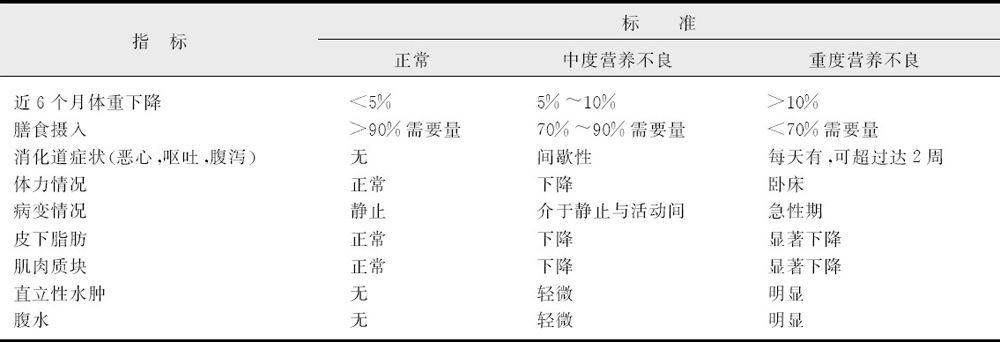
\includegraphics[width=5.92708in,height=6.28125in]{./images/Image00005.jpg}
\end{table}

急性发热性疾病病因很多,病史及临床表现典型者诊断较易,临床表现不典型的病例或较少见的疾病则会造成诊断的困难。因此,对于一时诊断未明的病例,鉴别诊断的思路要广,不但要熟悉常见病,也要了解少见病;不但要知道各种疾病的典型临床表现及实验室和辅助检查的诊断价值,也要不断积累在某特殊情况下临床表现不典型的疾病的诊断经验。本节主要讨论表\ref{tab2-1}中排黑体字的疾病,是在急性发热的鉴别诊断中较常遇到的疾病;以同时伴有皮疹为特征的急性发热性疾病放在“2.急性发疹性发热”一节中讨论;对伴有肺部病征的发热性疾病则只概要提及,详细讨论见“3.伴有肺部病征的急性发热”一节。

\protect\hypertarget{text00013.html}{}{}

\subsection{1.1 急性感染性发热}

急性感染性发热起病急,热度一般较高,多伴寒战或畏寒、全身肌肉和关节酸痛、头痛等毒血症状。一般可分为急性传染病和局限于某一脏器或组织的急性感染性疾病或(及)来源于局灶感染的败血症。前者往往有传染病的流行病学资料,后者多伴有局部症状和体征。细菌性感染多有周围血白细胞总数和中性粒细胞数升高。此外,血降钙素原(PCT)浓度>0.5ng/ml提示细菌感染,有助于与病毒感染、结核感染鉴别,且降钙素原水平与细菌感染的严重程度呈正相关。但也要注意降钙素原正常或轻度增高不能排除细菌感染的可能。而血清C反应蛋白在细菌感染时可呈中等度至明显升高。

\subsubsection{1.1.1 病毒性感染}

\paragraph{一、流行性感冒(流感)}

流行性感冒病毒可分为甲、乙、丙三型,其中甲型病毒易引起世界性流感大流行;乙型病毒则引起局部暴发和小流行;丙型病毒仅以散在形式出现。近几年新的病毒亚型如H5N1、H1N1和H7N9等出现流行或感染,需引起临床注意。

本病的潜伏期一般为1~7日,多数为2~4天。通常以突然畏寒、寒战、高热急骤起病,伴有全身酸痛、头痛、面潮红、结膜充血、虚弱无力等全身中毒表现,而呼吸道症状并不严重。血象白细胞总数减少,淋巴细胞相对增加。热程约3~5日。全身症状逐渐好转,但鼻塞、流涕、咽痛、干咳等上呼吸道症状逐渐显著。在流感多见的冬春季节,门诊上述症状的患者连续3日持续增加,并有直线上升趋势,或发热感冒患者2例以上的家庭连续增多,就应高度警惕本病的可能。对于非典型与散发病例,则易误诊为急性上呼吸道感染。但后者通常为非暴发流行、起病缓慢、症状较轻,上呼吸道症状较明显而无明显全身中毒症状。此外,流感亦易与多种早期的急性传染病如流行性脑脊髓膜炎、伤寒、副伤寒、支原体肺炎、军团菌病等相混淆,因此,须注意动态观察,以免造成误诊。

在流感流行时,根据接触史和典型临床表现诊断不难。特殊实验室检查可为确诊提供直接证据:①免疫荧光或免疫酶联染法检测抗原,取患者鼻洗液中黏膜上皮细胞涂片,用荧光或酶标记的流感病毒免疫血清染色检出抗原,快速且灵敏度高,有助于早期诊断。②用PCR测定流感病毒RNA,为直接、快速敏感的方法。③采样取患者起病3日内的含漱液或咽拭子做鸡胚接种或组织细胞接种培养分离病毒。④血清学检查:应用血凝抑制试验或补体结合试验检测急性期和恢复期(相隔2~4周)双份血清抗体效价,若升高4倍以上有诊断价值。

\paragraph{二、急性病毒性肝炎}

可有畏寒、发热,多呈中等度热,有些病例有明显的上呼吸道症状,类似感冒,少数患者出现关节痛,类似风湿热,应注意鉴别。但大多数患者有乏力、厌油、纳差、腹部不适或肝区、上腹部胀痛等症状。本期体征不显著或有肝大。故详细询问有无明显的消化道症状对诊断极有帮助。肝功能谷丙转氨酶升高,病毒性肝炎病毒检测或系列标志物的检测,有助于确诊。

\paragraph{三、流行性乙型脑炎(乙脑)}

初期典型表现为急性起病,早期发热,多为39℃以上高热,伴有头痛、恶心和呕吐,多有嗜睡和精神疲倦,可有抽搐,颈项强直。此后高热持续,出现意识障碍,如嗜睡、谵妄、昏迷、定向力障碍等,并出现惊厥或抽搐。有神经系统的体征如浅反射改变或脑膜刺激征,病理性锥体束征阳性等。轻型或普通型乙脑,可仅表现为头痛、发热、精神萎靡及嗜睡,此时常无神经系统体征,易致误诊。此时应仔细询问流行病学史[包括明显的季节性(7~9月份)、疫区、蚊虫叮咬史],脑脊液检查,血清补体结合试验、中和试验、血凝抑制试验和特异性IgM抗体测定有重要诊断价值。

\paragraph{四、脊髓灰质炎}

脊髓灰质炎发病的前驱期大多有发热,乏力不适,常伴有咽痛、咳嗽等上呼吸道症状。部分患者有恶心呕吐,腹痛腹泻等消化道症状。此期白细胞多数正常,而早期或合并感染时可增高,以中性粒细胞为主。上述表现无特异性,易误诊为上呼吸道感染或急性胃肠炎。但当发生在流行季节(夏秋季)如有易感者接触患者后出现上述症状应警惕本病。若发热不退,或热退后间歇1~6日,体温再次上升(称双峰热,为其典型的临床特征,见于10\%~30\%患者,小儿多见),并出现神经系统症状如头痛、肢体疼痛,感觉过敏,烦躁或嗜睡,体检出现颈背肌强直和阳性克氏征、布氏征,肌腱反射及浅反射减弱,则本病的可能性很大。此时脑脊液大多已有改变,呈无菌性炎症改变。与化脓性脑膜炎、结核性脑膜炎鉴别不难。但应注意与各种病毒性脑炎、流行性乙型脑炎鉴别。若出现弛缓性瘫痪则有利于本病的诊断。进入瘫痪期的本病患者,应与感染性多发性神经根炎鉴别。后者散发起病,不发热或仅有低热,逐渐出现弛缓性瘫痪,呈上行性、对称性,常伴感染障碍,脑脊液具有蛋白质增高而细胞少的分离现象为其特点。瘫痪恢复较快而完全,很少有后遗症。本病与引起轻瘫的其他病毒感染如柯萨奇、埃可病毒感染等区别,单从临床表现难以鉴别。确诊有赖于病毒分离及血清学检查。

确诊脊髓灰质炎需特殊的实验室检查:①病毒分离,起病1周内、从患者鼻咽部及粪便中分离出病毒,阳性率可达90\%,粪便可持续阳性2~3周。早期从血液和脑脊液中分离出病毒则更为可靠。②抗原检测:近年采用RT-PCR检测肠道病毒RNA,较组织培养快速敏感。③血清学检查:近年采用免疫荧光技术检测抗原及特异性IgM单克隆抗体酶标法检查,有助于早期诊断。

\paragraph{五、流行性出血热}

是一组以发热、出血、肾脏损害为主要临床表现的急性传染病。其病原体为汉坦病毒,鼠类为主要传染源。本病在我国全国各地均有报道,有明显季节性,有些地区该病流行高峰在5~6月份和10~12月份。

本病起病急骤,以畏寒、寒战、高热开始。体温可高达39~40℃,热型以弛张型为多。全身症状较重,表现为头痛、腰痛、眼眶痛(“三痛”)、畏光、视力模糊,颜面、上胸部及眼眶区明显充血(“三红”),似酒醉貌。

出血为常见症状,通常于发病第3~5日出现,皮肤黏膜、结膜、软腭、腋下可见散在针头大小的出血点或出血斑,有时密集的小点状出血排列成链条状,颇具诊断参考价值。出血点多见于上半身,尤其腋部与上胸部,这与一般紫癜不同。血小板大多减少,束臂试验每呈阳性。发热持续数天(一般3~7天),热退后症状反而加重并呈现低血压,有的甚至休克,为此病的重要特征之一。

患者有不同程度的肾脏损害表现。早期即可有蛋白尿及镜下血尿。有的病例在病程第5~7日可发生尿少甚至无尿,呈现急性肾小管坏死的病象,继而转入多尿期,以后逐渐康复。

本病典型的临床表现可达分为发热期、低血压期、少尿期、多尿期及恢复期五期。轻型病例病程较短,病情较轻。

本病早期应与上呼吸道感染、流行性感冒、伤寒、钩端螺旋体病等急性传染病及败血症相鉴别。有皮肤出血点应与血小板减少性紫癜相区别。当出现急性肾衰竭时,应与各种病因所致的急性肾衰竭相鉴别。本病有典型的临床表现和独特的临床经过,抗原检查和特异性抗体检查有助于早期诊断。近年采用多聚酶联反应(PCR)直接检测病毒抗原,有助于病原学诊断。

\paragraph{六、传染性单核细胞增多症}

本病是由EB病毒引起的一种急性或亚急性淋巴细胞良性增生的传染病。本病分布广泛,多呈散发性,以15~30岁的年龄组为多,流行性病例多见于儿童。发病多较急,多为中至高热,可呈弛张、不规则热或稽留热,热程自数日至数周。患者每有咽痛,咽峡炎相当常见,表现为咽、悬雍垂、扁桃体充血、肿大,其后可迅速出现斑状或膜状黄灰色苔膜,少数有溃疡和假膜形成。浅表淋巴结肿大亦相当常见,全身淋巴结均可累及,而以颈淋巴结肿大最为常见,通常无明显压痛。绝大多数病例有脾大,一般为轻中度肿大,约10\%患者有肝大并有肝功能异常,少数可出现黄疸。有时可出现斑疹或疱疹。病初起时白细胞计数正常,病后第10日左右白细胞总数有升高,分类中淋巴细胞增多;并出现异形淋巴细胞(10\%~30\%或更多)。本病病程多为1~3周,预后良好。

本病临床表现多种多样,常被误诊为急性咽炎、急性扁桃体炎、流感、病毒性肝炎、伤寒、血小板减少性紫癜、急性白血病或恶性淋巴瘤,少数神经系统受累者可误诊为乙型脑炎。周围血出现异形淋巴细胞(>10\%以上),是提示本病的重要线索。但异形淋巴细胞亦可见于某些其他病毒性感染如病毒性肝炎,流行性出血热等,但其数量一般<10\%。结合血清学检查可辅助诊断,嗜异凝集试验效价在1∶80以上具有诊断价值,若数周测定其效价上升4倍以上更有意义。但须注意,正常人、少数网状细胞瘤、单核细胞白血病、结核病亦可阳性,此时需吸附试验证实。

国外学者提出本病的诊断标准:①临床三联症:发热、咽峡炎、淋巴结病;②外周血淋巴细胞比例≥0.5和异形淋巴细胞比例≥0.1;③血清嗜异凝集抗体阳性。

\paragraph{七、巨细胞病毒感染}

正常成人巨细胞病毒(CMV)感染多表现为隐性感染,或单核细胞增多症表现,有发热、肝脾大,淋巴细胞相对或绝对增多,并出现异形淋巴细胞,与EB病毒所致的传染性单核细胞增多症相似,但巨细胞病毒感染咽痛和淋巴结肿大较少见,血清中无嗜异性凝集素及EB病毒抗体。免疫缺陷者的CMV感染,多发生在接受器官移植患者中,术后2~4个月多见,其首发临床表现为发热、乏力,可出现关节和肌肉疼痛以及全血细胞减少和异形淋巴细胞增多。病情进展快,肺部受累常见,可出现干咳、呼吸困难和进行性低氧血症,胸片两肺呈间质性、网状和结节状浸润,预后较差。检测特异性CMV-IgM抗体、CMV-DNA、CMV-PP65抗原阳性有助于急性和近期感染的诊断。血液或体液(主要为尿液)中分离出CMV病毒可确诊。

\paragraph{八、严重急性呼吸综合征}

严重急性呼吸综合征是2002年出现的由SARS冠状病毒(SARS-COV)引起的一种具有明显传染性、可累及多个脏器系统的特殊性肺炎,世界卫生组织(WHO)将其命名为严重急性呼吸综合征(SARS)。疫情暴发于温热带冬春之际,症状重,死亡率高。由于该病起病初期以发热为首发症状,呼吸道症状未出现或缺乏特异性,极易误诊为一般上呼吸道感染,如一旦延误诊断则会造成本病在与患者密切人群中的迅速播散。因此,在流行地区和流行季节要对本病保持高度警惕,有关本病的诊断与鉴别诊断参见第3.1节。

\protect\hypertarget{text00014.html}{}{}

\subsubsection{1.1.2 细菌性感染}

\paragraph{一、细菌性肺炎}

社区获得性肺炎常见细菌为肺炎链球菌、流感嗜血杆菌和卡他莫拉菌。患者常有受凉、劳累等诱因,通常急骤起病,以高热、寒战、咳嗽、血痰及胸痛为特征。本病早期或经抗生素治疗后上述症状和肺实变体征可不典型,易误导为未明原因的发热。因此,对心率和呼吸加速、血象白细胞总数增多者,应详细做胸部的体检。下叶肺炎刺激膈胸膜,胸痛可向腹部放射,易误诊为急腹症。胸部X线正侧位摄片,有助于早期做出诊断。

肺炎的临床诊断依据是:①新近出现的咳嗽、咳痰或原有呼吸道疾病症状加重,并出现脓性痰,伴或不伴胸痛。②发热。③肺实变体征和(或)闻及湿性啰音。④WBC>10×10\textsuperscript{9}
/L或<4×10\textsuperscript{9}
/L,伴或不伴细胞核左移。⑤胸部X线检查显示片状、斑片状浸润性阴影或间质性改变,伴或不伴胸腔积液。以上①~④项中任何1项加第⑤项,除外非感染性疾病可做出诊断。其他细菌或病原体引起的肺炎参见第3节。

\paragraph{二、感染性心内膜炎}

感染性心内膜炎指因细菌、真菌及其他微生物(如立克次体、衣原体等)直接感染心脏内膜表面,伴有赘生物形成。随着风湿性心脏病发病率的下降,风湿性心瓣膜病的感染性心内膜炎的发生率亦随之下降,而非风湿性瓣膜病的感染性心内膜炎发生率有所上升。加之,近年来日益增多的心血管疾病的创伤性检查、介入性治疗和人工心脏瓣膜的广泛应用,医源性感染性心内膜炎明显增加。静脉毒品滥用也增加了感染性心内膜炎的发病率。因此,对本病应保持警惕。

\subparagraph{(一)急性感染性心内膜炎}

本病常发生于原来无心脏病的患者。病原菌多为高毒力细菌和真菌,其中金黄色葡萄球菌约占50\%以上。本病往往起病突然,高热、寒战等全身毒血症状明显,病程常急骤凶险,易掩盖心内膜炎的局部临床表现。因心瓣膜和腱索的急剧损害,心脏可在短期内出现高调的杂音或原有杂音性质迅速改变,并可迅速发展为急性心力衰竭。故对败血症的患者,应注意心脏体征的改变,考虑本病的可能。如有多发性栓塞及多个器官、组织的转移性感染和脓肿出现,对诊断有重要提示。

累及右侧心脏的急性感染性心内膜炎,多见于安装心脏起搏器的老年患者,近年来由于静脉注射毒品成瘾者增多,右侧心脏心内膜炎的发病率亦明显增加。临床上除败血症表现外,常伴有咳嗽、胸痛、咳血痰和气急。累及三尖瓣者可闻及三尖瓣尖关闭不全的杂音,累及肺动脉瓣时可听到肺动脉瓣反流所致的舒张中期杂音。胸部X线可见多发性结节或片状炎症浸润,为三尖瓣或肺动脉瓣赘生物脱落所致的脓毒性肺梗塞。

急性感染性心内膜炎早期易漏诊,而后期病情危重,故诊断的关键是提高警惕,注意发现心脏及其他有关表现并密切观察病情变化。血培养和超声心动图对确诊有重要价值,详见下述。

\subparagraph{(二)亚急性感染性心内膜炎}

本病大多数发生在原有器质性心脏病的基础上,仅少数发生于正常的心脏。由于近年来普遍使用广谱抗生素,致病菌已发生明显改变,几乎所有的微生物都可引起本病,但草绿色链球菌仍是较常见的致病菌,肠球菌、表皮葡萄球菌、革兰氏阴性菌和真菌的比例则有增加。亚急性患者起病较缓慢。发热为最常见症状,以不规则热为多,也可为间歇热或弛张热,亦可仅有低热者。因此,原有器质性心脏病的患者发热一周以上,应考虑本病的可能。少数患者以贫血、顽固性心力衰竭、卒中、瘫痪、周围动脉栓塞等并发症的形式开始,因此,对原有心脏病患者,出现上述情况,亦应注意有否本病的存在。发热伴随的常见临床表现有皮肤黏膜瘀点、中等度贫血、蛋白尿和镜下血尿、脾大、心脏杂音等。白细胞数多数呈中度或轻度增高,少数可正常或减少,但分类中性粒细胞常增高。

由于近年来感染性心内膜炎的“经典”临床表现已不十分常见,尤其是皮肤和黏膜的瘀点、甲床下线状出血、Roth斑、Osler结、Janeway损害及杵状指(趾)的发生率较前明显下降,脾大的发生率亦已明显减少。而且有些症状和体征在病程晚期才出现。加之,患者多曾接受抗生素治疗,给细菌学诊断带来一定困难。因此,在临床工作中应对本病提高警惕,对患有心瓣膜病、先天性心脏病、人造瓣膜置换术、安装心脏起搏器和静脉滥用毒品者,在不明原因发热超过一周以上,应怀疑本病的可能,立即做血培养。若兼有贫血,周围栓塞现象和心脏杂音的出现,应考虑本病的诊断。

本病的临床表现可涉及全身多脏器,既多样化,又缺乏特异性,需注意与多种疾病进行鉴别。如败血症、疟疾、伤寒、左房黏液瘤等。对不典型病例应提高警惕,细心观察病情变化,密切注意心脏杂音性质的改变。

血培养和超声心动图是确诊感染性心内膜炎的两大手段。阳性血培养结果结合超声心动图发现赘生物、瓣周并发症等是心内膜炎的确诊依据。血培养采血方法,对急性患者应在入院后3小时内,每隔1小时1次共采集3个血标本后开始抗菌治疗;对未经治疗的亚急性患者,应在第1日每隔1小时1次共采集3个血标本,如次日未发现细菌生长,则重复采血3次后再开始治疗;对已用过抗生素的亚急性患者,停药2~7天后采血。骨髓培养可提高阳性率。对累及右侧心脏的心内膜炎患者,经食管超声心动图可提高赘生物的检出率。修订的Duke诊断标准见表\ref{tab2-2}。符合2项主要标准,或1项主要标准+3项次要标准,或5项次要标准为确诊;符合1项主要标准+1项次要标准,或3项次要标准为疑诊。

\begin{table}[htbp]
\centering
\caption{感染性心内膜炎Duke诊断标准(修订版)}
\label{tab2-2}
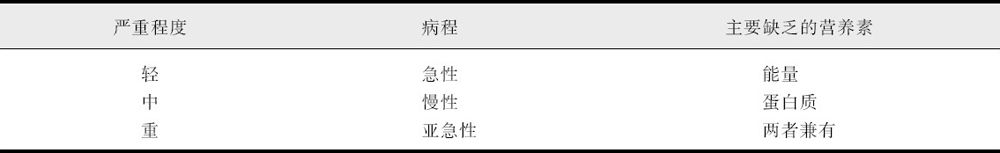
\includegraphics[width=5.91667in,height=3.44792in]{./images/Image00006.jpg}
\end{table}

\paragraph{三、急性肾盂肾炎}

本病多见于女性,尤其是生育年龄的妇女,而糖尿病患者及使用导尿管等装置的老年患者亦不少见。当患者有急起畏寒、发热,伴有腰痛、尿频、尿急、尿痛时,应考虑急性肾盂肾炎的可能。若尿常规检查证实有脓尿,则诊断大致可以成立。病原学的诊断有待细菌培养证实。若仅有高热而尿路症状不明显者,应与各种发热性疾病相鉴别。腹痛、腰痛明显者应与急性胆囊炎、阑尾炎、盆腔炎、肾周围脓肿等鉴别。一般经多次尿液检查即能诊断。B超或CT检查有助于胆囊炎和肾周脓肿的诊断。

\paragraph{四、急性胆道感染}

急性发热者伴有上腹绞痛时,应考虑急性胆道感染的可能,通过进一步检查诊断一般不困难(参见第78.1节)。老年患者由于疼痛的敏感性降低,可无胆绞痛的主诉,但胆囊区仍可有明显的压痛。本病应与急性病毒性肝炎、急性胰腺炎、左下肺炎、急性肾盂肾炎等疾病相鉴别。血清转氨酶及病毒性肝炎系列标志物、血和尿淀粉酶、X线胸片和尿液检查则有利于各自的诊断。B超、CT检查可发现胆系结石和梗阻。

\paragraph{五、细菌性肝脓肿}

寒战、高热、肝区痛或右上腹痛,体检肝大并有压痛或(及)肝区叩击痛,血象白细胞总数及中性粒细胞增加,应考虑本病。B超有助诊断,必要时在B超引导下行肝穿刺抽出脓液可确立诊断。阿米巴肝脓肿临床上与细菌性肝脓肿相似,但阿米巴肝脓肿起病较慢、病程较长、慢性消耗表现较常见,而高热及白细胞增多则较不明显,部分病例有痢疾史或证实有阿米巴肠病。B超引导下肝脓肿穿刺,典型阿米巴肝脓肿脓液为巧克力样,在抽脓最后部分近脓腔壁的脓液有可能找到滋养体。近年,无论是细菌性肝脓肿还是阿米巴肝脓肿临床表现不典型病例增多,常发生漏诊,应提高警惕。肝脓肿还要与肝癌(特别是肝癌中心坏死液化合并感染)、肝囊肿或肝包囊虫病合并感染、右膈下脓肿等疾病鉴别(参见第106.2节及第106.3节)。

\paragraph{六、其他急性局灶性细菌感染}

此类疾病的共同特点是高热、畏寒或寒战,周围血象白细胞和中性粒细胞增多,并有局部症状和体征。

\subparagraph{(一)膈下脓肿}

通常并发于腹腔化脓性感染或腹腔手术后,尤其是急性阑尾炎、胃及十二指肠穿孔、胆囊切除术、脾切除术后等。肝脓肿亦可直接向右膈下组织蔓延。若有上述情况,患者又出现寒战、高热、白细胞总数和中性粒细胞增高,又未能找到其他感染灶时,应想到此病的可能。膈下脓肿以右侧多见,患者自觉患侧上腹部有显著搏动性疼痛,以深呼吸或体位转动时加重,患侧下胸部常有局部皮肤水肿并有压痛及叩击痛,听诊呼吸音减弱或消失。站立位X线检查可发现患侧膈肌上升活动受限,反应性胸膜炎,患侧膈下可见液平面或气泡。B超或CT检查可早期明确诊断。

\subparagraph{(二)肾周围炎或肾周脓肿}

患者常以畏寒、发热或寒战高热开始,伴有患侧肾区疼痛,并向同侧下腹及大腿内侧放射,脊肋角显著压痛及叩击痛。当此病早期未出现肾周围局部体征时易误诊为全身感染或急性肾盂肾炎,及时进行B超或CT检查可明确诊断。

\subparagraph{(三)其他局灶性感染}

化脓性中耳炎、化脓性扁桃体炎、化脓性关节炎、化脓性骨髓炎以及其他各部位的浅部化脓性感染(如疖、皮下急性蜂窝织炎等)或深部化脓性感染(如臀肌脓肿、脑脓肿等)均可引起急性高热,局灶性症状和体征可提示诊断。

\paragraph{七、败血症}

败血症(septicemia)是指病原菌及其毒素侵入血流所引起的临床综合征,是一种严重的血流感染。尽管目前对败血症的定义仍有争议,但疾病国际分类(ICD)仍采用败血症这一病名。当患者有原发感染灶,出现全身性脓毒症症状,并有多发性迁徙性脓肿时提示败血症。值得注意的是有时原发的感染病灶可能很轻微或已愈合。因此,临床上遇到不明原因的急性高热,伴有畏寒或寒战、出汗,全身中毒症状重,白细胞总数和中性粒细胞明显增高,而无特殊症状、体征及流行病学病史提示急性传染病时,应考虑败血症的可能。医院内感染败血症绝大多数见于有严重基础疾病如各种血液病、肝及肾衰竭、晚期恶性肿瘤,或医源性感染如各种导管的长期置留、透析疗法等,如患者出现不明原因发热或(及)病情恶化时应注意败血症的可能。阳性血培养是诊断败血症的重要依据,反复多次做血培养可获得较高的阳性率。

根据我国近年对败血症病原学分析的报道,我国败血症的病原体以金黄色葡萄球菌、大肠杆菌和其他肠道阴性杆菌为多见,但表皮葡萄球菌、铜绿假单胞菌及一些耐药菌败血症有增加趋势,厌氧菌及真菌败血症亦非罕见。不同病原菌所造成的败血症临床表现可有一定差异,兹分述如下:

\subparagraph{(一)需氧革兰氏阳性球菌败血症}

\hypertarget{text00014.htmlux5cux23CHP2-5-1-2-7-1-1}{}
1.金黄色葡萄球菌败血症

此病较常见,国内对各地共1000余例次败血症的病原学分析表明,金黄色葡萄球菌败血症所占比例高达20\%~30\%。临床急起发病,常先有畏寒或寒战,继而高热、头痛与出汗,多伴有恶心呕吐、腹泻、全身肌肉及关节疼痛,皮疹形态多样化,可有瘀点、荨麻疹、猩红热样皮疹及脓疱疹等。迁徙性化脓病灶是本病的特点,对病因诊断有重要意义。迁徙性病灶以四肢和躯干的多发性软组织脓肿、多发性肺脓肿、脓胸、肝脓肿、化脓性脑膜炎、骨髓炎等多见。本病并发心内膜炎者可高达8\%。临床若遇发热持续不退,体检发现有心脏病理杂音的出现,伴有进行性贫血、反复出现皮肤瘀点、内脏血管栓塞、血培养持续阳性,应考虑心内膜炎的存在,及时做超声心动图有助确诊。

金黄色葡萄球菌败血症的诊断一般不难,当存在原发性皮肤化脓性病灶或导管插管处红肿热痛,出现寒战、高热等中毒症状时,首先应考虑本病的可能。若同时伴有皮疹与迁徙病灶,则可能性更大。但临床上部分患者急起发热,病史不清,会造或诊断困难。如当胸片发现多发性迁徙肺脓肿者,此时易误诊为肺炎;胸片有片状模糊阴影者,易误诊为肺结核;少数患者白细胞计数较低,发热呈稽留热时,可误诊为伤寒。提高对本病的警惕和认识。早期多次血培养有助于及早做出诊断。

\hypertarget{text00014.htmlux5cux23CHP2-5-1-2-7-1-2}{}
2.表皮葡萄球菌败血症

近年来本病逐渐增多,目前约占败血症总数的10\%~15\%,且70\%为医院内感染。常见于体内异物留置或植入者(如静脉导管、人工关节、人工瓣膜、起搏器等)。由于表皮葡萄球菌为正常皮肤表面的细菌,血培养假阳性率高,因此,血培养阳性难以鉴别是否为污染所致。然而当患者发热不退,体内留有异物(如静脉导管)处局部皮肤红肿、压痛,或人工瓣膜患者出现新的杂音或多发性血栓形成等,都是感染的有力证据。另外,双份(身体左右侧静脉)血培养同时阳性意义更大。

\hypertarget{text00014.htmlux5cux23CHP2-5-1-2-7-1-3}{}
3.肠球菌败血症

本病发病率近年未有明显增多的趋势,77\%为医院内感染,占院内感染败血症的10\%左右。病原菌常来源于泌尿生殖道,亦易发生于消化道肿瘤及腹腔感染的患者,因此,对有上述病史的急性发热患者,尤其是院内感染,要考虑本病的可能。由于本病对多种抗菌药物耐药,故病情多危重。

\subparagraph{(二)需氧革兰氏阴性杆菌败血症}

约占败血症总数的40\%左右,其中,最常见为大肠杆菌败血症,其次为肺炎克雷伯杆菌、铜绿假单胞菌和其他肠杆菌败血症。病原菌常从泌尿生殖道、肠道(尤其是下消化道)或胆道入侵,多见于一般体质较差,伴有各种影响机体免疫功能的原发病。热型不一,以弛张热多见,少数患者可有体温不升、双峰热。40\%患者可发生休克,休克的特点是出现早且持续时间较长,严重患者可出现多脏器功能损害。多数患者白细胞增高,少数患者正常或减少但常有中性粒细胞左移现象。本病与金黄色葡萄球菌败血症在临床上虽然很相似,但原发灶不同,早期出现休克以及迁徙病灶较少见,有临床鉴别价值。

铜绿假单胞菌败血症通常继发于重度烧伤、白血病、淋巴瘤、各种恶性实体瘤以及气管切开、静脉导管、导尿等。临床表现较一般革兰氏阳性杆菌败血症凶险,可有较特征性中心坏死性皮疹。患者淡绿色尿(绿球蛋白)可作为铜绿假单胞菌败血症的诊断佐证。

\subparagraph{(三)细菌L型败血症}

细菌在体内多种因素影响下失去细胞壁变为L型,临床上常在应用抗生素后产生。细菌转变为L型后临床表现与原菌感染不同,其常见临床表现为发热波动难以控制,多呈弛张热(占80\%)。胸片示间质性肺炎但呼吸道症状轻微,尤其是感染性发热应用抗生素后一度有效,以后发热起伏波动,白细胞总数不高而有核左移和中毒颗粒者。临床上L型细菌以金黄色葡萄球菌多见,因此,在无法确定其类型的情况下,可选择对L型金葡菌有效的抗生素进行试验性治疗。多次高渗及等渗双份血培养均培养出L型细菌可助确诊。

\subparagraph{(四)厌氧菌败血症}

厌氧菌多从肠道肿瘤、发炎的憩室、女性生殖道、压疮、感染的胆道等处入侵血流,常发生于有严重基础病免疫功能低下的患者。厌氧菌多与需氧菌同时混合感染。对有上述情况,敏感抗生素治疗效果不佳甚至恶化的败血症患者,应考虑厌氧菌混合感染的可能,应加做厌氧菌特殊培养以助诊断。病变组织有脏而臭的分泌物、含气体、有假膜形成是诊断的佐证。

\subparagraph{(五)真菌败血症}

主要以念珠菌感染为主,近年来发病率明显增高,绝大部分为机体抵抗力低下的医院内感染,常见于长期接受广谱抗生素、糖皮质激素、免疫抑制剂或肿瘤化疗患者。因此,对具有上述易感因素,持续高热,经足量高效抗生素治疗96小时无效,尤其存在真菌感染灶(如口腔黏膜、皮肤)者应警惕本病的可能。血培养发现真菌可确诊,但阳性率不足50\%,且培养费时较长。因此,对高度怀疑本病者,选择广谱的抗真菌药物治疗症状改善,体温下降至正常者,亦为有力的佐证。

\paragraph{八、结核病}

发热为结核病最常见的全身性毒性症状,多数为长期低热,但当病灶急剧进展扩散时则可出现高热,呈稽留热或弛张热热型,可伴有畏寒,但很少寒战。临床上属此类型者有急性粟粒型结核,某些肺外结核如网状内皮系统结核(无反应结核病)、结核性脑膜炎、浸润型肺结核。

\subparagraph{(一)急性粟粒型结核(急性血行播散型肺结核)}

急性粟粒型结核来源于自体结核病灶,当机体免疫功能低下时加重和恶化,并从血流播散。本病发病急骤,持续高热为早期或突出症状,中毒症状严重,有时伴有乏力、畏寒等非特异症状。由于临床上肺部粟粒型结核多见,患者常伴有咳嗽、咳痰、气短等呼吸道症状。病程中可伴有轻度肝脾大。周围血象中多数有白细胞减少,少数有全血细胞减少。亦有少数病例白细胞明显增高呈类白血病反应。本病早期胸部X线表现不明显或阴性时,易误诊为伤寒、败血症或恶性血液病。但本病患者常有呼吸道症状如咳嗽、气促等症状,且血象无相对的淋巴细胞增多,肥达反应阴性,多次血培养伤寒杆菌阴性可与伤寒鉴别。反复多次血培养无致病菌生长,高效广谱抗生素治疗无效,可与败血症鉴别。全血细胞减少又伴有肝脾大者,易与白细胞不增高的急性白血病或恶性组织细胞病混淆。本病在发病第一、二周内,由于病变太小,在胸片上不易发现病灶。因此,对怀疑本病者,若一次胸片阴性,应定期复查或行胸部高分辨CT检查,可发现典型的两侧肺野内大小相等、从肺尖到肺底均匀一致的粟粒状致密影。结核菌素试验阳性对诊断有参考价值,但阴性不能否定结核,特别是老年人或免疫功能低下的患者。此外,眼底检查近半数成人病例,可发现脉络膜上有灰白色或黄色圆形小结节,对本病的诊断极有帮助。

\subparagraph{(二)无反应结核}

属特殊类型结核病,见于免疫力严重低下患者,其特点为:①全身中毒症状较重,持续高热,故又称之为结核性败血症;②呼吸道症状出现较晚;③肝、脾、淋巴结肿大多见且早期出现;④可并发粒细胞缺乏甚至全血细胞减少,亦可呈类白血病反应;⑤合并肺门淋巴结或纵隔阴影增大者可高达72\%。本病临床上易与风湿性疾病、败血症、伤寒病、血液病和恶性淋巴瘤混淆,定期复查胸片或胸部CT,痰、淋巴结穿刺物涂片检出抗酸菌有助确诊。

\paragraph{九、伤寒与副伤寒}

\subparagraph{1.伤寒}

发热是伤寒的早期症状,有时为唯一症状,因此是未明原因发热经常要考虑的疾病之一。凡发热持续一周以上原因未明者,需注意伤寒的可能。传统观点认为具有诊断参考价值的临床表现有:①热型早期呈梯形上升,极期呈稽留热型持续,后期呈弛张型缓解,病程多为3~4周;②伤寒毒血状态,表现为表情淡漠,无欲面容;③相对缓脉与重脉;④发病一周左右胸前、腹上区分批出现少数玫瑰疹;⑤脾轻度肿大;⑥白细胞总数减少,相对淋巴细胞增多,嗜酸性粒细胞减少或消失。

近年来,我国伤寒的发病率已明显降低,其流行高峰亦已较为平坦,并发症已显著减少,且由于起病早期多已接受过抗菌药物治疗而致临床表现多不典型。因此,依靠流行病学资料和典型临床表现作出伤寒的临床诊断往往有困难,关键是要注意伤寒的可能。确诊主要靠病原学和血清学检查:①一周后肥达反应“O”抗体凝集效价≥1∶80,H抗体凝集效价≥1∶160,有诊断参考价值,病程中效价逐渐升高意义更大。但血清学诊断需密切结合临床,凝集效价持续阴性,不能作为否定伤寒的依据。②血、骨髓培养伤寒杆菌阳性是确诊的依据,尿、粪培养阳性可弥补血、骨髓培养的不足。

临床上对高度怀疑伤寒患者,亦可试用氟喹诺酮类、氯霉素、氨苄西林等进行诊断性治疗。用药后本病多在3~5日内体温逐渐下降,临床症状亦迅速好转。

\subparagraph{2.副伤寒}

流行病学特点与伤寒相同,但发病率远较伤寒低。副伤寒甲、乙临床表现难与伤寒鉴别,但副伤寒潜伏期较短,急性起病较多,早期胃肠炎症状较明显,热型不如伤寒典型。副伤寒丙可表现为轻型伤寒,急性胃肠炎或脓毒症。与伤寒相同,确诊有赖于病原学及血清学检查,但要注意副伤寒丙的血清凝集效价较低,少数患者可始终阴性。

\hypertarget{text00014.htmlux5cux23CHP2-5-1-2-10}{}
十、细菌性心包炎

结核性或化脓性心包炎:早期症状不典型,诊断较困难。因此,对不明原因的发热兼有心前区疼痛的患者,应想到本病的可能。体检发现心尖搏动弱,心脏扩大,心音遥远,应考虑本病。若心前区闻及心包摩擦音,可作出初步临床诊断。本病的心前区痛与急性心肌梗死疼痛类似,应注意鉴别。心电图、胸部X线有助诊断,心脏B超和心包穿刺可确诊。

\hypertarget{text00014.htmlux5cux23CHP2-5-1-2-11}{}
十一、兔热病

本病是土拉杆菌所致的急性传染病,属自然疫源性疾病,在我国见于西藏、青海、内蒙古、黑龙江及山东等地。主要传染源是野兔,其次是鼠类和羊。由直接接触,烹食未熟受染的野兔、松鼠及其他啮齿类动物,或被壁虱叮咬而受染。潜伏期一般为3~4日,起病大多急骤,高热伴寒战及毒血症状如头痛、肌肉酸痛,局部皮肤出现丘疹,继而化脓,坏死中心脱落而形成溃疡,边缘隆起有硬结感,伴有一定程度的疼痛。白细胞总数多正常,偶有轻度升高。土拉杆菌抗原皮内试验或荧光抗体试验有助于早期诊断。

兔热病分溃疡型和腺型、肺型、胃肠型、伤寒型或中毒型、眼腺型、咽腺型等不同类型。确诊有赖于血或病灶分泌物的细菌分离(特殊培养或动物接种)及阳性免疫反应。

本病应与鼠疫、炭疽、鼠咬热等的皮肤病灶和腺肿鉴别。尚应与各种肺炎、伤寒、结核、布鲁菌病、类鼻疽、组织胞浆菌病等相鉴别。

\hypertarget{text00014.htmlux5cux23CHP2-5-1-2-12}{}
十二、人感染猪链球菌病

猪链球菌病是由多种不同群的致病性链球菌引起的一种人畜共患传染性疾病,人感染猪链球菌并引起发病的情况比较少见,其传染源主要为猪链球菌感染的病猪和带菌猪,高危人群为屠宰、饲养生猪或加工、销售、运送猪肉类的人员,感染途径主要通过接触病死猪时致病菌经破损皮肤和黏膜侵入人体,或吃了未完全煮熟的病猪肉或内脏而感染,目前尚未发现人与人之间的传播。

人感染猪链球菌病潜伏期短,平均2~3天,可短至数小时,最长达7天。临床上可分为四种类型:普通型、休克型、脑膜炎型和混合型。起病急,临床表现为畏寒、发热、头痛、头昏等全身中毒症状。重症病例迅速进展为中毒性休克综合征,出现皮肤出血点、瘀点、瘀斑,血压下降,脉压差缩小;可表现出凝血功能障碍、肝、肾功能不全、急性呼吸窘迫综合征、软组织坏死,筋膜炎等。部分病例表现为脑膜炎,恶心、呕吐、昏迷,脑膜刺激征阳性,脑脊液呈化脓性改变。还有少数病例为混合型,即在中毒性休克综合征基础上,出现化脓性脑膜炎表现。部分病例在恢复期出现听力减弱、障碍。实验室检查外周血白细胞计数升高(严重患者发病初期白细胞可以降低或正常),中性粒细胞比例升高。诊断上结合疫情资料、流行病学调查资料和患者的发病情况、临床症状及早期病例的尸检报告可做出初步诊断;进一步的确诊有赖于实验室病原学诊断。

\protect\hypertarget{text00015.html}{}{}

\subsubsection{1.1.3 钩端螺旋体病}

鼠和猪是本病的主要传染源,其带有钩端螺旋体的尿可以污染各种水源,人与污染的水源接触,钩端螺旋体通过暴露部位的皮肤进入人体而造成感染。全国各地均有本病报道,但以南方各省多见。本病具有如下流行病学特点:①疫水接触史,患者在起病3~20天内到过鼠类出没或猪尿污染的污水沟、稻田,皮肤曾与污水接触。散发病例,因很多场所被污染,有时无明确接触史而常被误诊。②主要流行于夏秋收割季节,有时可在洪水过后造成流行。③患者多为青壮年农民、饲养员,外地进入疫区者亦易患病。本病临床表现复杂,临床表现轻重不一,轻者似感冒,仅表现为轻度发热。典型的临床特点为:早期有高热,全身酸痛,结膜充血,腓肠肌压痛及浅表淋巴结肿大等类似败血症的表现。中期为肝、肾、肺等多器官损害与功能紊乱。

本病可分为流感伤寒型、肺出血型、黄疸出血型、肾衰竭型和脑膜炎型。流感伤寒型多数以全身症状为特征,起病急骤,畏寒发热,头痛、全身肌痛并有鼻塞、咽痛、咳嗽等,而无黄疸和中枢神经系统症状,肺亦无明显病变,易误诊为流行性感冒、上呼吸道感染。但本病患者往往同时或随之出现肝、肾功能损害,半数有皮肤黏膜出血,不支持流感和上呼吸道感染。仔细调查流行病史有助于鉴别诊断。肺出血型应与肺结核、支气管扩张、肺肿瘤鉴别。通过胸部X线或CT等检查加以区别。黄疸型易误诊为黄疸型肝炎,但后者以纳差为主,无眼结合膜充血和腓肠肌压痛,ALT、AST明显升高,而CPK不高,病毒性肝炎系列标志物和流行病学史可资鉴别。肾衰竭型与流行性出血热临床表现有相似之处,但后者通常有酒醉貌,无腓肠肌压痛,流行性出血热特异性抗体和病毒抗原检查有助于两者鉴别。脑膜脑炎型的钩端螺旋体病与乙脑都在夏秋季流行,但后者无全身酸痛、结膜充血和腓肠肌压痛,且乙脑抽搐、昏迷等脑部症状较钩端螺旋体病明显,尿常规、肝功能多正常。

对于钩端螺旋体病的病原学诊断,应用暗视野显微镜可直接检查患者血、尿及脑脊液等标本中的钩端螺旋体。病原体分离可用体液培养或动物接种技术。血清补体结合试验和凝集溶解试验自病程第一周末开始升高,在第三、四周达高峰,间隔两周双份血清,效价增高4倍以上有诊断价值。酶联免疫吸附试验比凝溶试验阳性出现更早和更灵敏,有早期诊断价值。

\protect\hypertarget{text00016.html}{}{}

\subsubsection{1.1.4 立克次体感染}

\paragraph{一、斑疹伤寒}

流行性斑疹伤寒在我国已基本得到控制;地方性斑疹伤寒由鼠蚤传播,属自然疫源性疾病,国内以河南、河北、山东和辽宁等地报道的病例较多,以夏秋收割季节发生较多。本病以高热、剧烈头痛、全身肌痛起病,眼结膜充血,可有中枢神经系统临床表现。早期病例需与流感、流行性出血热、钩端螺旋体病、伤寒、恙虫病、流行性脑脊膜炎、大叶性肺炎等疾病鉴别。一旦典型皮疹出现(一般在4~6天内),则病象相当明显,参见第2.1节。

\paragraph{二、恙虫病}

恙虫病流行于夏秋季,患者在疫区的田野或草地上工作、卧息时,可因被受染恙螨叮咬而感染。流行季节有不明原因急性发热患者,要警惕本病的可能。须追查流行病学史与细致搜寻焦痂,参见第2.1节。

\protect\hypertarget{text00017.html}{}{}

\subsubsection{1.1.5 寄生虫感染}

\paragraph{一、疟 疾}

间日疟和三日疟具有间歇性、规律性、发作性寒战、高热和大汗,伴有贫血和肝脾大等典型的临床表现,诊断不难。而恶性疟疾的临床症状较复杂而多样化,发热前寒战较少,热型多不规则,热后较少出汗。伴头痛、肌痛、纳差等症状,常有恶心、呕吐、腹泻等消化道症状。高热患者常有剧烈头痛,并出现谵妄、抽搐和昏迷,脑膜刺激征明显(脑型疟疾),易误诊为乙型脑炎。部分恶性疟患者有相对缓脉,加之有脾大和白细胞减少,易与伤寒相混淆。因此,在到过疟疾流行地区后出现不明原因的发热,应警惕疟疾的可能。疟原虫的发现是诊断疟疾的主要依据,一次血片检查阴性不能否定,应在发作过程中反复检验。在发热前的畏寒期采血作厚滴片检查,可提高阳性率。血片阴性时可作骨髓涂片检查,其阳性率较血片为高。氯喹或奎宁对疟疾治疗有特效,一般用药后1~2天体温下降,症状基本控制,对高度疑似的病例可用常规剂量作诊断性治疗。

\paragraph{二、阿米巴肝脓肿}

见前述及参见第106.3节。

\paragraph{三、急性血吸虫病}

本病多发生于夏秋季,有严格的地区性,多见于初次接触疫水感染者,但慢性血吸虫患者在再次大量感染后亦可表现为急性感染。平均潜伏期40日左右,其间可出现疫水接触处皮肤发痒,红色小丘疹约1~2日消失。急性患者都有发热,发热的高低、热型、热程与感染轻重因个体反应不同而异。可高热持续不退,伴精神萎靡、意识淡漠,重听、腹胀、可有相对缓脉而误诊为伤寒,但白细胞总数增高及分类中嗜酸性粒细胞增多(一般占20\%~40\%),据此可与伤寒鉴别。急性血吸虫患者有肝大,伴不同程度压痛,以左叶为著,与肝脓肿相似,但B超、CT发现占位病变可资区别。血吸虫卵所造成的异位肺损害,除有呼吸道症状外,胸片常示两肺中下野、大小略不等粟粒点状影应与粟粒型结核相鉴别。肠道症状表现为腹泻、腹痛、黏液血便,部分患者可出现腹膜刺激征,腹部饱满,有柔软感和压痛,类似结核性腹膜炎。凡夏秋季接触疫水,病初出现尾蚴皮炎,具有发热、肝大伴压痛、腹痛腹泻,而血中嗜酸性粒细胞明显增高者,需考虑急性血吸虫病的诊断。但不典型和重笃病例可不出现嗜酸性粒细胞增高或反而减少,据此,亦不能完全否定急性血吸虫病的可能。下述检查有助于确立急性血吸虫病的诊断:

1.血清免疫学检查

(1)抗体检测:常用检测方法有环卵沉淀试验(COPT)、间接血凝试验(IHA)、酶联免疫吸附试验(ELISA)等。COPT法目前仍为疫区广泛应用。近年来建立的简便快速的ELISA方法、敏感度达90\%以上,且敏感性和重现性好。但应注意抗体检测法不能区别既往感染与现症患者。

(2)抗原检测:可证实活动性感染。单克隆抗体斑点酶联法检测循环抗原敏感性和特异均较高,其临床应用尚在进一步研究中。

2.目前采用尼龙袋新鲜粪便集卵孵化法,提高了阳性率,为主要的检查方法。但一次阴性不能轻易除外本病,宜反复多次进行,以获得病原学的诊断。

3.直肠黏膜活组织检查,可提高检出虫卵的阳性率。

\paragraph{四、旋毛虫病}

猪为人体旋毛虫感染的主要传染源。本病发病前1~2周有生食或半生食含旋毛虫幼虫包囊的猪肉史,初期主要为肠炎症状,如腹痛、腹泻和稀水便;急性期发热多在38~40℃之间,热型多为弛张热,也可呈不规则热,伴有肌肉疼痛和水肿、皮肤斑丘疹或猩红热皮疹等,血象白细胞和嗜酸性粒细胞增高,确诊有赖于胸大肌或腓肠肌肌肉活检找到梭形包囊和幼虫和(或)免疫学检查等。

\protect\hypertarget{text00018.html}{}{}

\subsubsection{附:丝虫病}

丝虫病系由丝虫寄生于淋巴组织、皮下组织或浆膜腔所致的传染病。淋巴丝虫病是由班氏、马来或帝汶丝虫寄生于淋巴组织所致的传染病。我国除山东、台湾为单纯班氏丝虫流行外,其余地区均有两种丝虫病流行。在丝虫病疫区,患者有发热、淋巴管(结)炎、阴囊内器官与组织炎症或象皮肿,血中嗜酸性粒细胞增多,须考虑丝虫病。

班氏丝虫寄生于深部或浅表淋巴结、淋巴管中,尤以腹腔、盆腔、腹膜后组织、肾盂、附睾、精索等部位为多。因此,除有肢体淋巴管炎外,尤以阴囊内器官与组织的炎症病变为多见,阻塞胸导管或乳糜池可致乳糜尿。马来丝虫主要寄生于人体四肢浅部淋巴系统,尤以下肢多见,因此,肢体淋巴管炎和象皮肿较明显,无乳糜尿及外生殖器局部病征,巨型象皮肿亦较少见。帝汶丝虫病主要表现为腹股沟、股及沿大隐静脉和其分支的淋巴管炎、淋巴结炎及膝部以下象皮肿。

丝虫病发热的特点是往往呈不规则的周期性发作,通常伴淋巴管、淋巴结炎。少数病例的淋巴管炎位于腹内深处,可无浅表病理体征。有些病例如阴囊内器官与组织炎症,在急性发作期疼痛可先从下腹部开始,或向腹部放射,故易误诊为阑尾炎或其他急腹症,但体检时腹部体征阴性而阴囊内有器官与组织炎症存在,可资鉴别。此外,精索与附睾炎要与附睾结核鉴别,后者结节在附睾内,常粘连在一起,不痛,少有反复发作。

病原学检查发现微丝蚴为确诊的直接证据。于晚间熟睡时采周围血作成厚涂片,每夜连续2~3次,检出率可达90\%以上。有实验条件者,采用间接荧光抗体或酶联免疫吸附试验可检测丝虫特异抗体。对疑似病例,服用乙胺嗪后肢体淋巴管或阴囊内出现新结节,或阴囊内原有病变增大、疼痛加剧,对丝虫病的诊断有一定的辅助诊断价值。

1994年,全国864个流行县、市(含班氏和马来丝虫病)全部达到基本消灭丝虫病标准,实现全国基本消灭丝虫病的目标。

\protect\hypertarget{text00019.html}{}{}

\subsection{1.2 非感染性急性发热疾病}

\subsubsection{一、风湿热}

风湿热是一种常见的反复发作的急性或慢性全身性结缔组织炎症,主要累及心肌、关节、中枢神经系统、皮肤和皮下组织。本病最常见于5~15岁的儿童和青少年,多数患者发病前1~5周先有咽炎或扁桃体炎等上呼吸道感染史。

风湿热患者多有低热,中等度热,亦可呈现高热。部分病例没有明显关节痛或关节炎的症状、以发热为主要临床表现,诊断有时困难。

迄今风湿热尚无特异性的诊断方法,主要依靠临床表现与动态观察,辅以实验室检查。临床上沿用修订的Jones诊断标准,认为具有下述2项主要表现或1项主要表现加2项次要表现,并先前有链球菌感染的证据,可诊断风湿热。

主要表现:①心脏炎:为临床上最重要的表现,其特征有:a.心肌炎,最早的临床表现为二尖瓣和主动脉瓣的器质性杂音。心尖区第一心音常减弱,常可闻及奔马律;b.心动过速,常>100次/分,与体温不成比例;c.心脏扩大;d.心律失常及心电图异常,常见为房室传导阻滞、期前收缩和心电图PR间期延长;e.心力衰竭,往往由急性心肌炎所致,尤其多见于年龄较小的患者;f.心包炎,出现于风湿热活动期,为严重心脏炎的表现之一。②多发性关节炎。③舞蹈病。④环形红斑。⑤皮下结节。

次要表现:①关节痛;②发热;③急性反应物改变(血沉降率增快,C反应蛋白增高);④心电图PR间期延长;⑤既往风湿热史和现患风心病。

有链球菌感染证据:①近期患过猩红热;②咽喉拭子培养或快速链球菌抗原试验阳性;③链球菌抗体效价升高。

在上述5项主要表现中,心脏炎和多发性关节炎的诊断意义最大。但亦非特异性。风湿热累及心肌时,表现为与发热不相称的心动过速和心电图异常改变,常有诊断参考价值。但由于也非特异性,亦需在鉴别的基础上考虑诊断。由于多关节炎的疾病种类繁多,多关节痛在几乎所有发热性疾病中经常可见,临床工作中,易将有类似表现的骨、关节和其他风湿性疾病如系统性红斑狼疮等误诊为风湿性关节炎,应予以重视。另一方面,约有1/4风湿热患者无多关节炎症状,甚至无关节痛,据此就不考虑风湿热的诊断,是另外一种错误倾向,应有所认识。风湿性心包炎的心包摩擦音,由于持续时间短暂,易被忽略而漏诊。主要表现中的后3项,发生率甚低,在诊断中起作用少。但少数患者尤其是儿童出现舞蹈病,结合某项其他表现,则有可靠的诊断价值。

上述的实验室检查是诊断风湿热的参考条件,但必须结合临床资料综合分析。抗“O”滴度>500U,认为有参考诊断价值,但不能作为确诊的依据。因为其阳性率仅有70\%~80\%,且仅表示新近有过链球菌感染,ESR在合并严重的心力衰竭时可以正常。部分风湿热患者白细胞计数增高。心电图有P-R间期延长、不完全性或完全性房室传导阻滞,多源性或多发性期前收缩、二联律、阵发性心动过速或房颤,QT间期延长有较大的参考诊断价值。但其心电图改变亦非经常出现,需定期反复复查才能发现异常,且上述心电图改变亦非风湿热特有。

1992年美国心脏病学会对Jones标准又进行了修订:该标准保留了Jones原5项主要表现,减去1项次要表现(既往风湿热史和现患风心病),并指出有下列3种情况时可不必严格执行该标准,即:①舞蹈病者;②隐匿发病或缓慢发展的心脏炎;③有风湿热病史或现患风心病,当再次感染A族链球菌有风湿热复发的高度危险性者。

患有风湿性心脏病患者有发热时,须考虑风湿性心内膜炎与亚急性细菌性心内膜炎两者的鉴别。后者多见于原有心瓣膜病,有进行性贫血、脾大、瘀点、瘀斑,可有脑、肾、肺等不同部位的栓塞症状。反复血培养阳性,超声心动图在瓣膜上发现赘生物可资鉴别。对已证实合并亚急性细菌性心内膜炎的风湿性心脏病患者,经足量抗生素治疗症状无改善或一度改善后又恶化,下列表现提示有风湿活动:①上呼吸道感染出现心悸、气促、病程超过半月以上者;②原因不明的难于纠正的进行性心力衰竭或急性肺水肿;③ESR增快,心力衰竭时ESR正常,心衰好转后ESR反而增快;④洋地黄治疗效果不好或耐受量降低易出现中毒症状;⑤不明原因的心律失常;⑥原有器质性心脏杂音性质的改变;⑦出现心脏以外的风湿性病变如风湿性脑病、脉管炎、关节炎、环形红斑等。此时做抗心肌抗体检测,心脏炎者阳性率达70\%,特异性高,抗A组链球菌胞壁多糖抗体(ASP)明显升高,阳性率达80\%以上,有助于判断风湿活动和其他心脏病鉴别。

如发热患者伴多关节炎、ESR增快,也可见于诸多结缔组织病、结核性关节炎或结核感染反应性关节炎、各种败血症引起的感染性关节炎或关节痛。此外,风湿热还要与SLE、成人Still病、莱姆病(Lyme病)、急性白血病,链球菌感染后状态等鉴别。

近年来风湿热、风湿性关节炎已明显减少,典型病例已不多见。但轻症、不典型病例仍可见到,给诊断带来一定的困难。

\subsubsection{二、系统性红斑狼疮}

部分系统性红斑狼疮早期可仅以发热为突出症状,其他系统受累的症状和体征可以不明显,诊断有一定困难。未明原因的无菌性急性发热,尤其是生育年龄的妇女,应考虑到本病的可能,并作进一步相关检查,参见第5.3节。

\subsubsection{三、急性白血病}

临床上凡患者急起发热兼有进行性贫血及(或)出血倾向,须考虑急性白血病的可能性。典型的急性白血病有持续发热、出汗、衰弱、出血倾向、进行性贫血、胸骨压痛,肝、脾及(或)淋巴结肿大,周围血细胞高度增多(也可正常或减少),以原始白细胞占优势,血培养阴性等表现。根据血象与骨髓象通常不难作出诊断。有的病例须与类白血病反应相区别,参见第5.2节。

\subsubsection{四、热射病}

热射病(包括日射病)亦称中暑性高热。表现为高热(>40℃)和神志障碍。本病基本上发生于高温季节,临床上可分为两种类型:劳力性和非劳力性(或典型性)。前者主要是在高温环境下内源性产热过多;后者主要在高温环境下体温调节障碍引起散热减少。

\paragraph{1.劳力性}

其特点是在高温环境和无风天气下进行体力劳动或剧烈运动时发病,多见于平素健康的年轻人。早期有头痛、乏力、恶心、口渴、心烦、少汗或多汗等非特异症状,继而急骤发病,体温急剧升高至40℃以上,皮肤灼热干燥,心率可达160~180次/分。脉压增大,可发生谵妄、抽搐、昏迷、出现病理神经反射。此种患者可发生横纹肌溶解和多器官功能衰竭,甚至死亡。

\paragraph{2.非劳力性}

在高温环境下,多见于居住拥挤和通风不良的城市老年人、产妇、体弱或患慢性病者。表现为皮肤干热、发红、无汗。病初可有各种行为异常和癫痫发作,继而可发生谵妄、昏迷、瞳孔对称缩小,终末期散大,严重者可出现低血压、休克、心律失常及心力衰竭、肺水肿、脑水肿。

根据病史和体征,本病一般不难诊断。尤其患者有高温接触史,出现昏迷和体温过高时应考虑热射病的可能。在诊断本病前应与脑炎、脑膜炎、脑型疟疾、脓毒病、脑血管意外、产褥热、甲状腺危象、抗胆碱能药物中毒及其他急性感染性疾病相鉴别。

\subsubsection{五、药物热}

药物热是机体对药物的一种超敏反应。常与特异性体质有关。患者往往先有感染,在给药后7~10天出现发热,多为低热或中等度发热,也可表现为高热。药物热大多数伴有药物皮疹或荨麻疹、肌肉关节痛,但有少数病例仅表现为发热,无皮疹及其他症状,一般情况好。药物热一般在停药后48小时内热退。再用该药,则在数小时内再次引起发热。药物热应与感染性疾病感染未能控制及风湿性疾病、肿瘤引起的发热相鉴别。

\subsubsection{六、恶性高热}

恶性高热是使用全身麻醉剂产生的严重并发症。麻醉剂以肌肉松弛剂和吸入性麻醉剂合用时发生率更高。家族性遗传性体质缺陷是内在的重要因素,其中以遗传性肌病更为重要。本病常在麻醉后立即发生,心律不齐是早期表现,常伴呼吸困难、发绀,常伴全身骨骼肌强直。高热或特高热是必有的主要症状,可高达40℃以上。高热期间血清肌酸磷酸激酶、丙氨酸基转移酶、乳酸脱氢酶增高,还可出现肌红蛋白血症,尿中出现肌红蛋白。常因心力衰竭、脑水肿、急性肾功能衰竭而死亡。诱发恶性高热的药物有琥珀酸胆碱、氟烷、乙醚、环丙烷、氯仿、甲氧氟烷、氯胺酮、氨氟醚等。

本病应与甲状腺功能亢进危象、嗜铬细胞瘤及恶性综合征等相区别。恶性综合征是抗精神病药物治疗特有而罕见的严重反应,主要表现为持续高热、肌肉僵硬、意识障碍及心血管症状等,可导致死亡。

\subsubsection{七、组织坏死性淋巴结炎}

组织坏死性淋巴结炎又称Kikuchi病,1972年由日本人首先报道,是一种主要累及淋巴结的良性、自限性、全身性疾病,误诊率较高,可达30\%~40\%。本病好发于青年女性,近年发病率有上升趋势,多累及颈部淋巴结,也可多部位先后出现淋巴结肿大,直径多在0.5~2.5cm;肿大淋巴结活动、无粘连,伴疼痛或压痛;发病前多有类感冒症状,体温38~39.8℃,抗生素治疗无效;实验室检查发现外周血白细胞计数在正常范围内或降低,血沉升高,PPD试验阴性。活检淋巴结破碎是特征之一。本病糖皮质激素有效是其特点,自然病程1~4个月。

\protect\hypertarget{text00020.html}{}{}

\subsection{1.3 急性“未明热”}

有少数急性发热患者未能查明原因,这些急性“未明热”以夏、秋二季为多见,且多见于年轻人。这些患者有急性感染的全身症状、体检及实验室检查无异常发现,病程通常在一周左右,预后良好。但是“未明热”仅为少数,有些病例由于检查未能周详及受设备条件或目前的认识所限,一时未能作出病因诊断,故诊断要慎重。必须除外引起急性发热的器质性疾病,首先要考虑病毒感染,其次为细菌感染如顿挫型伤寒、潜在的肺外结核、某些隐蔽的肿瘤等均要仔细排除。

\protect\hypertarget{text00021.html}{}{}

\section{2 急性发疹性发热}

在临床工作中,皮疹是常见的体征,据统计有100多种疾病发热伴有皮疹,常见有急性发疹性传染病、结缔组织病、变态反应性疾病、血液病等。一些原因不明的发热性疾病亦可发生皮疹,由于在不同疾病,皮疹可有不同形状,发疹时间及伴随症状也不相同。因此,可作为不同疾病鉴别诊断的一个重要体征(表\ref{tab2-3})。

\begin{table}[htbp]
\centering
\caption{急性发疹性发热性疾病的分类}
\label{tab2-3}
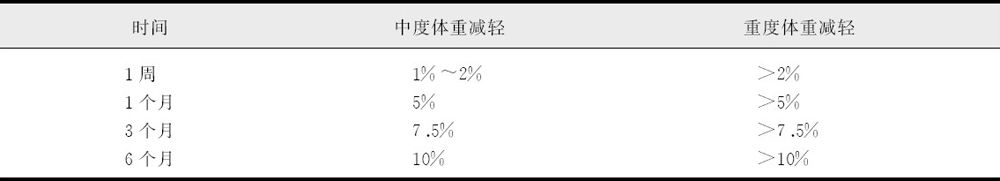
\includegraphics[width=5.9375in,height=1.84375in]{./images/Image00007.jpg}
\end{table}

\subsection{2.1 急性发疹性传染病}

急性发疹性传染病均有一定的潜伏期,掌握出疹的时间及其与发热的关系、出疹的部位及顺序、皮疹的性质及其相关体征、病程的经过,在鉴别诊断中有重要意义。

\subsubsection{一、麻 疹}

多在冬春二季流行,以儿童为多见。潜伏期为7~14天,发热3~5日出疹,主要症状有发热及上呼吸道卡他症状,同时有眼结膜充血、流泪、畏光日渐加重的表现,在发病第2~3日又可于双侧近臼齿颊黏膜处出现细砂样灰白色小点,绕以红晕,称麻疹黏膜斑,为本病早期特征。起病3~5日后,全身症状及上呼吸道症状加重,体温再度升高可达40℃,皮疹先于耳后发际出现,然后迅速发展到面部,自上而下蔓延直至手心足底;皮疹为淡红色、散在,然后密集呈鲜红色,持续约5日左右。皮疹出齐后按出疹顺序隐退、脱屑、色素沉着、整个病程10~14日。上述皮疹的临床表现,结合流行病史,血象白细胞计数正常或减少,80\%~90\%患者鼻咽、眼分泌物涂片染色镜检可发现脱落的上皮多核巨细胞、并可寻找到特异性麻疹抗原可诊断。从上述分泌物或血液白细胞中分离到麻疹病毒则可确定诊断。

在近期接受过免疫抑制剂或接种过疫苗者,全身症状轻、皮疹散在、不留色素,甚至可无皮疹和口腔黏膜斑。出血性皮疹多见于免疫力低下的重型患者。

成人麻疹的临床表现与儿童大致相同,但一般中毒症状较重,并发症也不少,且以呼吸道并发症多见。

麻疹需与风疹、猩红热、药疹等相区别。

\subsubsection{二、风 疹}

潜伏期较长为14~21天左右,主要发生于儿童,亦可见于青少年。临床症状较麻疹轻,发热仅1~2天,起病后即有皮疹出现,分布于颜面部,迅速波及躯干部,皮疹呈现玫瑰色斑丘疹,可融合成片。体温随皮疹的出现而上升,但较少超过39℃,通常2~3天内退热。其重要体征为伴有耳后、枕部甚至全身淋巴结肿大,无压痛。与麻疹的皮疹不同的是,皮疹的消退和发展同样迅速,疹退时体温亦下降,肿大的淋巴结亦逐渐恢复。皮疹消退后一般不留色素沉着,亦不脱屑。

风疹早期白细胞总数减少,淋巴细胞增多,并出现异形淋巴细胞,浆细胞增多,特异性风疹抗体IgM阳性有诊断意义。

风疹患者的皮疹形态介于麻疹与猩红热之间,因此,应着重对此三种常见的发热性出疹性疾病进行鉴别诊断。流行病学资料对鉴别诊断有重要帮助。

\subsubsection{三、传染性红斑}

本病病原为B19病毒,发病多见于儿童,少数亦可见于成人。潜伏期为4~12天,皮疹在第1~2天出现,最初为颊部水性红斑。后为全身斑丘疹,呈环形、网状,常有痒感,四肢亦可出现对称性斑丘疹,但罕见于手掌和足底。往往能同时出现发热、上呼吸道症状、肌痛和胃肠道症状。血清或咽拭子检测到特异性IgM抗体可确立诊断。本病需与药物疹、风疹和猩红热相鉴别。

\subsubsection{四、水 痘}

水痘是由于水痘带状疱疹病毒引起的急性传染病,多见于小儿,其潜伏期为10~24天。皮疹常于发病数小时或1~2天内分批出现,往往同时出现发热、头痛、咽痛、四肢酸痛和胃肠道症状。皮疹先见于躯干,逐渐延及面部,最后达四肢。皮疹呈向心性分布,以躯干为多,面部及四肢较少。皮疹发展快为本病的特征之一,开始为粉红色帽针头大的斑疹,数小时内变为丘疹;再经数小时变为水疱。短者这一过程仅6~8小时。水痘初呈清澈水珠状,以后稍混浊,壁薄易破,疱疹在24小时内开始皱缩、结痂。痂皮脱落后遗留浅瘢痕。水痘典型病例诊断不难,必要时可作血清学补体结合试验,出疹后1~4日即出现补体结合抗体阳性,可协助诊断。近年应用PCR方法检测鼻咽部分泌物VZVDNA,为敏感和快速的早期诊断手段。

水痘主要与轻症天花相鉴别,其鉴别要点如表\ref{tab2-4}。

\begin{table}[htbp]
\centering
\caption{水痘与天花的鉴别诊断}
\label{tab2-4}
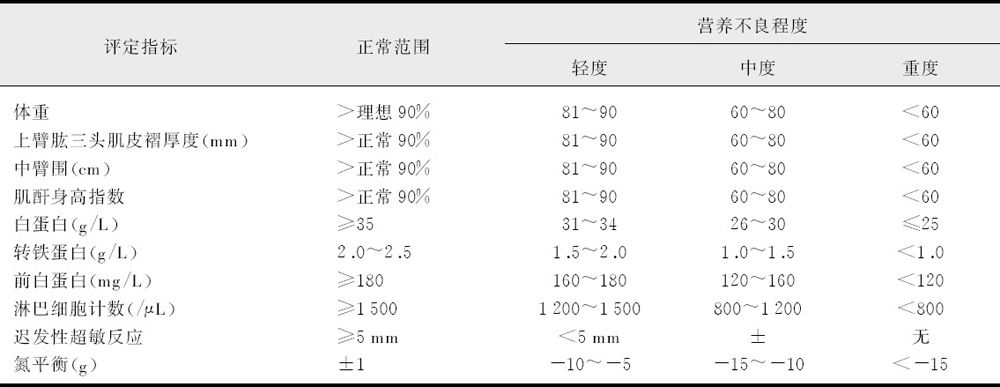
\includegraphics[width=6.04167in,height=3.8125in]{./images/Image00008.jpg}
\end{table}

\subsubsection{五、登革热}

登革热为登革病毒引起,经蚊传播的急性传染病,多流行于夏秋季节。潜伏期2~15日。其临床特征为双相热、剧烈头痛、皮疹、肌肉骨关节剧烈酸痛、淋巴结肿大、白细胞和血小板减少、淋巴细胞相对增多。

本病多数起病急骤,常以畏寒发热开始,颜面及眼结膜显著充血,颈及上胸皮肤潮红,发热持续2~4天即退,皮疹常于发病后2~5天出现。初见于掌心、脚底或先发生于躯干及腹部。然后蔓延至全身。皮疹呈麻疹样,少数呈猩红热样,或介于两者之间,压之褪色。体温下降者此时又可再次上升(呈马鞍热)。皮疹于1~5日(平均3日)消失,体温同时下降。整个病程约5~7日。本病确诊有赖于病毒分离。目前国内用酶联免疫吸附试验检测特异性IgM抗体,对早期诊断有较大的意义。PCR方法检测登革热病毒RNA,具有快速、敏感性高、特异性强的优点。

\subsubsection{六、斑疹伤寒}

斑疹伤寒可分为流行性斑疹伤寒和地方性斑疹伤寒,两者临床特征相近似,但后者病情较轻,病程亦较短,皮疹很少呈出血性。

典型的斑疹伤寒,流行于冬春季节,其潜伏期为5~21天,常急骤起病,体温于第2~4天即达高峰(39~40℃),呈稽留高热型,伴有速脉(与体温升高程度呈正比)、头痛、周身肌肉痛、眼结膜及脸部充血。皮疹于病程第4~6日出现,为本病重要体征,见于80\%以上病例。初见于胸背、腋窝、上臂两侧,1日内迅速波及全身。而面部及下肢皮疹较少。但可出现于手心和足底,皮疹初为鲜红色,继而转为暗红或瘀点状。神经系统症状明显且出现早,头痛、呆滞、神志迟钝,加之患者有脾大,酷似伤寒。但本病一般无相对缓脉,血、粪培养阳性可资区别。部分流行性斑疹伤寒有腓肠肌压痛、肝大、黄疸和肾损害,少数伴有出血皮疹,在南方地区易与钩端螺旋体病混淆。但后者有疫水接触史,有全身出血倾向,皮肤出血而非呈斑丘疹状,白细胞增高,ESR增快,血清凝溶试验阳性可资鉴别。

流行性斑疹伤寒的诊断有赖于血清学检查:①外斐试验其凝集效价>1∶320,有参考诊断价值,因为非立克次体病变等也可出现阳性反应,但效价较低。复发型斑疹伤寒外斐试验往往阴性或效价<1∶160,故有鉴别诊断价值。②以提纯的普氏立克次体颗粒性抗原作补体结合试验,不仅具群特异性,且具种特异性,可区别流行性斑疹伤寒和地方性斑疹伤寒。③以可溶性抗原作立克次体凝集试验,特异性高,操作简便,可用于与其他群立克次体区别。且流行性斑疹伤寒的凝集抗体为IgM,复发型斑疹伤寒为IgG,两者可作鉴别。④分子生物学检查,用DNA探针或PCR方法检测普氏立克次体特异性DNA,具快速、特异、灵敏等优点,但作为诊断依据时,仍需结合临床表现和流行病学资料作出判断。

流行性斑疹伤寒与地方性斑疹伤寒的鉴别见表\ref{tab2-5}。

\begin{table}[htbp]
\centering
\caption{流行性斑疹伤寒与地方性斑疹伤寒的鉴别}
\label{tab2-5}
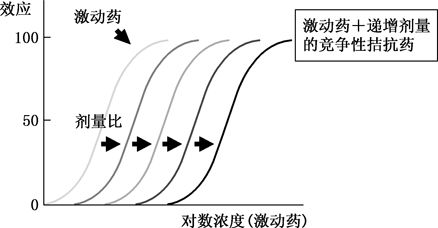
\includegraphics[width=5.94792in,height=1.67708in]{./images/Image00009.jpg}
\end{table}

斑疹伤寒还应与伤寒、回归热、流行性脑膜炎,流行性出血热、恙虫病、麻疹等鉴别。依据流行病学史及相关的实验室检查,一般可作出鉴别诊断,与伤寒的鉴别见表\ref{tab2-6}。

\begin{table}[htbp]
\centering
\caption{斑疹伤寒与伤寒的鉴别}
\label{tab2-6}
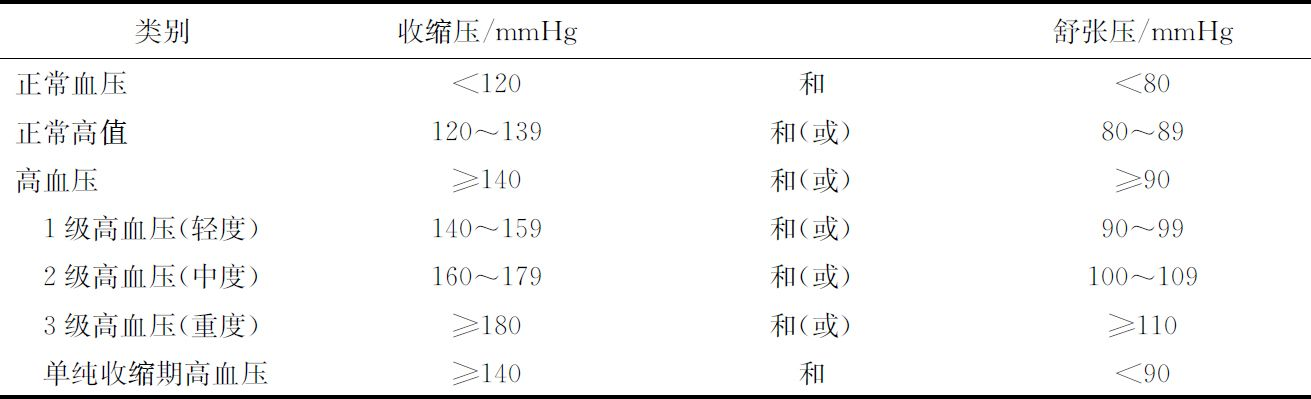
\includegraphics[width=5.95833in,height=3.45833in]{./images/Image00010.jpg}
\end{table}

\subsubsection{七、恙虫病}

恙虫病的潜伏期为5~20日,流行于夏秋季节,农民、与草地接触频繁的青少年及从事野外劳动者易得此病。起病多突然、体温迅速上升,达39~40℃,伴寒战、头痛、四肢酸痛、颜面潮红、结膜充血,类似斑疹伤寒的面容。严重者有谵妄、重听、腹胀、神志改变,部分患者可发生肠出血,易误诊为伤寒。焦痂和溃疡为本病的特殊体征,见于65\%~98\%患者。焦痂多见于腋窝、腹股沟、会阴、外生殖器、肛门等处。幼虫叮咬处出现红色丘疹,成水疱后破裂,中央坏死,结痂呈褐色或黑色,痂皮脱落后成小溃疡,边缘略隆起,底部为淡红色肉芽肿。因焦痂与溃疡无痒痛,发生于隐蔽部位,易被忽略。但仔细体检,往往可发现焦痂或溃疡,其附近的淋巴结肿大疼痛,有助于本病的诊断。

皮疹的发生率自30\%~100\%不等,为斑疹或斑丘疹,暗红色,压之即退色。皮疹多见于胸背和腹部,向四肢发展,面部很少,手掌脚底无疹,此点有助于与斑疹伤寒的鉴别。

血清免疫学检查:①外斐试验:患者血清可与变形杆菌oxk株发生凝集反应,阳性率70\%~80\%,滴度递升有诊断价值;②补体结合试验,特异性和敏感性较外斐试验高。

分子生物学检查:PCR检测恙虫病立克次体Sta58或Sta56抗原基因片段的方法诊断价值更高。

\subsubsection{八、猫抓病}

本病是汉赛巴通体经猫抓、咬人体后侵入而引起的传染病。主要临床表现为被猫抓咬后3~10日,局部出现红斑性丘疹,少数丘疹转为水疱或脓疱,少数可穿破形成小溃疡,可留下短暂色素沉着或结痂而愈。体检可发现抓伤感染部位引流区域淋巴结肿大。全身症较轻,半数患者有发热(>38.3℃)及出现胃肠道症状、头痛和结膜炎。结膜炎可伴耳前淋巴结肿大为本病重要体征之一。

本病病变部位的焦痂与溃疡须与恙虫病鉴别,后者的临床症状重,并发症多,焦痂和溃疡多在隐蔽部位,血白细胞增高,流行病学史有助于鉴别。

本病确诊有赖于淋巴结或皮损处的活检涂片中发现汉赛巴通体。

\subsubsection{九、猩红热}

猩红热是乙型溶血性链球菌引起的急性传染病,流行于冬春两季,早期软腭上有小米粒状红疹或出血点,常在皮疹出现之前出现,可提示早期诊断。典型病例以寒战高热起病,伴咽峡炎。患者于起病第2天出现弥漫充血基础上的点状(针尖大小)猩红色斑疹,自胸上部与颈底部开始,继而波及全身,严重者皮疹可为出血性,有瘙痒感。皮疹以躯干、皮肤皱褶处、大腿内侧为多,面部仅有发红而无皮疹,唇周反现苍白,即所谓猩红热面容,皮疹消退后,有大片脱皮现象,如见于病程后期亦有诊断价值。此外,患者有咽痛、杨梅舌等。血象白细胞增多,病程第一、二周后,可有嗜酸性粒细胞增多趋势。恢复期少数病例可并发肾炎与中毒性神经炎等。

猩红热无特异性的实验室检查:咽拭子培养可发现溶血性链球菌,但无特异性,阳性结果须结合临床考虑。皮疹消退试验:于皮疹处皮内注射猩红热抗毒素0.1ml或恢复期血清0.5ml,注射部位皮疹在6~8小时消退,有助猩红热的诊断。

猩红热须与风疹、麻疹、药疹、类猩红热鉴别(表\ref{tab2-7})。

\begin{table}[htbp]
\centering
\caption{猩红热、麻疹、风疹、药疹的鉴别}
\label{tab2-7}
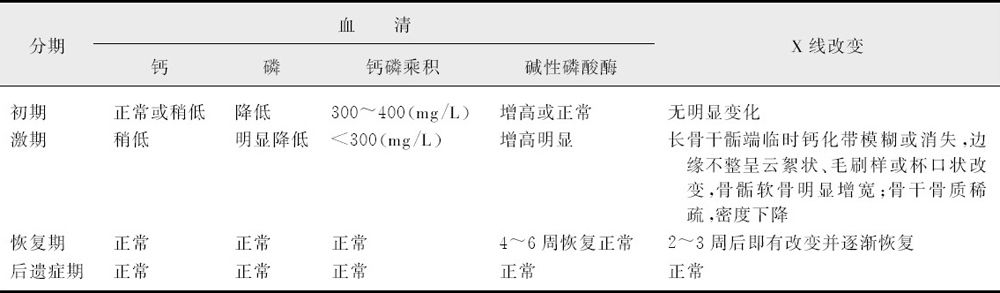
\includegraphics[width=5.97917in,height=3.92708in]{./images/Image00011.jpg}
\end{table}

\subsubsection{十、伤寒、副伤寒}

伤寒、副伤寒的皮疹为玫瑰疹,约20\%~40\%患者于病程第7~13日出疹。分批出现。副伤寒的玫瑰疹出现较伤寒早,有时数量较多,但玫瑰疹的发生率较少,且不典型,易被忽视,需注意与其他肠道革兰氏阴性杆菌败血症鉴别。确诊有赖于血、骨髓、粪便培养。肥达反应也有参考价值。

\subsubsection{十一、丹 毒}

丹毒是由β溶血性链球菌侵入后引起皮肤及其网状淋巴管的急性炎症。起病急、高热、寒战和全身不适。其皮肤病变好发于下肢和面部,局部烧灼样痛,片状红疹,中间较淡,边缘清,略隆起,有时形成水疱,内含浆液样液体。血象白细胞增高,分类左移。以水疱中抽取浆液样液体作涂片和培养,可发现溶血性链球菌,对确诊有重要价值。

丹毒需与急性蜂窝织炎区别,后者是皮筋膜下、肌间隙或深部蜂窝组织的急性弥漫性化脓性感染,炎症病变部位较深在,迅速扩散,边缘不隆起,界限不清,全身症状较明显,且有原发感染灶可寻。

发生于肢体的丹毒尚需与丝虫病淋巴管炎相区别。丹毒及其他细菌性淋巴管(结)炎,局部皮肤红肿疼痛剧烈,压痛明显,全身中毒症状明显。病灶发展呈向心性,远端皮肤有破损。通常不在同一部位反复发作,局部无硬结。丝虫病淋巴管(结)炎,局部淋巴结肿大疼痛,淋巴管肿胀从近端向远端扩展,晚期表现为淋巴管阻塞,炎症反复出现。若为班氏丝虫病,还可引起精索炎、附睾丸和睾丸炎。腹股沟处的淋巴结有硬结感。本病早期白细胞轻度增高,嗜酸性粒细胞显著增多。

丹毒还需与类丹毒相区别,类丹毒是由于感染猪丹毒的红斑丹毒丝菌引起。本病是一种职业病,主要由于与受污染的生肉(主要为猪肉)接触而发生感染。好发于屠宰工人和炊事员,外伤为诱因。病变多局限在接触的手与手指,虽然皮肤损害与丹毒相似,但与丹毒好发于下肢和面部不同。类丹毒颜色略呈青红,不起水疱,逐渐向周围发展。全身中毒症状不如丹毒明显。只有少数严重病例,皮疹波及全身时,才有发热。

\subsubsection{十二、兔热病}

兔热病绝大多数地区的主要传染源是野兔,其次是鼠类和羊。人类通过直接接触或吃了未煮熟的含菌兔肉或为鼠粪污染的食物和饮水而受染。皮肤感染局部形成红斑或丘疹,继而化脓坏死,中心脱落形成溃疡,边缘隆起而有硬结感。流行病学史,特别是有野兔接触史及相关职业等均有重要参考意义,确诊有赖于细菌分离和阳性免疫反应。

\subsubsection{十三、鼻 疽}

鼻疽是由马鼻伯克菌引起的感染性疾病,马科动物是主要传染源,患者发病前有与马直接和间接接触史。细菌从皮肤破损处进入,形成一个小结节,伴全身症状,急骤畏寒高热,病程进展,感染部位呈蜂窝织炎,进而有坏死的溃疡形成。当细菌从黏膜进入体内时,可引起眼、鼻和口腔感染继而出现溃疡和肉芽肿性病变。严重病例首先出现全身丘疹,随后发展为全身脓疱,侵入血液而形成败血症。

本病临床表现复杂,常不易确诊。必须结合接触病兽和实验室接触病菌史,分泌物涂片中荧光抗体阳性或各种培养物分离病菌,为主要诊断依据。血清学试验阳性有助于诊断。

本病须与类鼻疽、孢子丝菌病、链球菌蜂窝织炎和败血症鉴别。

类鼻疽是类鼻疽伯克菌引起的人畜共患的疾病,临床表现与鼻疽极为相似,局部化脓感染表现为皮肤破损处结节形成,引流区域淋巴结肿大和淋巴管炎,常伴畏寒发热和全身不适。急性肺部感染是类鼻疽最常见的类型,肺部炎症多见于上叶,呈实变,并常有薄壁空洞形成,易误诊为结核病。此型可发展为败血症。

病原学检查:以渗出物、脓液作染片和培养、悬滴试验可观察到动力,可以与马鼻疽伯克菌区别。尿中类鼻疽伯克菌抗原检测、胶乳凝集试验灵敏性较差,但特异性强;酶联免疫吸附试验灵敏性和特异均较高,可作为确诊的依据。

\subsubsection{十四、莱姆病(Lyme病)}

莱姆病是一种蜱媒螺旋体病,本病的传染源主要是野生和驯养的哺乳动物,啮齿动物中的白足鼠、哺乳动物中的鹿更为重要。当人的皮肤被蜱叮咬以后,出现慢性移行性红斑。开始时为一个红色斑疹或丘疹,然后逐渐扩大形成一片大的圆形皮损,外缘有鲜红边界,皮损早期中央有时呈致密红斑、硬变、疱疹、坏死。一般经2~3周皮损自行消退。50\%~80\%可并发多关节炎,11\%~15\%表现为神经系统广泛受累,表现为脑脊髓膜炎、颅神经炎、舞蹈病、小脑共济失调、脊髓炎等。且常先于关节症状出现,8\%~10\%患者有心脏受累(以房室传导受累多见、少数患者有房颤和心包炎),约10\%患者有肝炎样症状与体征。本病的多关节炎、舞蹈病需与风湿热鉴别。出现神经系统的并发症时,应与原发于神经系统本身的疾病区别。

本病的诊断主要依据流行病学资料与临床表现,慢性移行红斑具有重要诊断价值。血清学的诊断以酶联免疫吸附试验最为灵敏。特异性抗体效价>1∶200具诊断价值。血、脑脊液、皮肤活检标本培养阳性,则可确诊。

\protect\hypertarget{text00022.html}{}{}

\subsection{2.2 风湿性疾病}

\subsubsection{一、风湿热}

临床上约有1/3的风湿热患者在病程中有皮疹出现,具有诊断意义的为环形红斑和皮下结节。环形红斑少见,发生率为3\%~5\%,为淡红色红晕,中央苍白,不痛不痒,压之退色,多见于躯干和四肢近端,红斑初时较小,继而迅速向周围扩大,边缘略隆起,几个红斑融合可形成较大、不规则的圆圈,常为一过性,出现快,消失亦快。

皮下结节,亦少见,发生率不到2\%,结节多位于肘、膝、枕部、前额、棘突等骨质隆起或肌腱附着处,如豌豆大小,结节坚硬、无痛,与皮肤不粘连。

其他皮疹如荨麻疹、多形红斑、结节红斑等亦可见到,无特异性诊断价值。

\subsubsection{二、系统性红斑狼疮(SLE)}

约80\%~85\%SLE患者有皮疹,皮肤损害为多形性。颜面蝶形红斑,周围红斑和指(趾)甲远端下红斑具有特征性,常出现较早,前者是诊断本病的一个重要病征。其他皮肤损害有斑丘疹、水疱、大疱和血疱,日光暴晒后加重(光敏感)为本病的另一重要病征。有时可出现荨麻疹样损害。由于有部分SLE患者早期可无皮肤损害,而以发热或关节炎为首发症状,易误诊为败血症和风湿性关节炎。本病白细胞不高或减少,分类无左移可与败血症区别,SLE自身抗体,如抗核抗体(ANA)敏感性高达95\%,是SLE最佳的筛选试验,抗双链DNA抗体和抗Sm抗体特异性高,阳性有确诊价值。据此可与风湿性关节炎鉴别。

\subsubsection{三、急性皮肌炎}

本病较少见,皮肤和肌肉受累是导致本病的两组主要症状,皮损往往先于肌病发生。发热可为本病的初发症状,故早期诊断有一定困难,本病的皮疹为多形性,通常在面部尤其是上眼睑发生紫红色斑,逐渐向前额、颧、耳前、颈上胸部V字区扩展。闭眼近睑缘处可见明显扩张的枝状毛细血管,以眼睑为中心出现眶周水肿性红色斑片,具有一定的特征性,掌指关节和指间关节伸面出现红色丘疹、斑疹,以后萎缩、色素减退,上覆盖细小鳞屑,可见溃疡,称Gottron征,亦具特征性。肌肉往往四肢肌肉首先累及,近端重于远端,肩胛带和骨盆肌肉通常最早累及,上臂和股部肌群次之,其他部位肌群更次之。病变呈对称性。由于全身任何部位皆可受侵犯,故患者可出现肌肉疼痛,肌力下降,各种运动功能障碍和特殊姿态,如不能坐立,步态拙劣,伸展困难。面肌运动障碍,可出现张口受限,缺乏表情。

急性皮肌炎的免疫学检查可发现血清中肌浆球蛋白抗体,阳性率为90\%,其他结缔组织病此抗体阴性。血清肌酸磷酸激酶(CPK)、醛缩酶、AST、ALT、LDH均增高,且与肌肉病变的消退平行。上述血清肌浆酶的测定中,以CPK和醛缩酶最为敏感。借此可与SLE、类风湿关节炎、硬皮病鉴别。尿肌酸测定,皮肌炎患者24小时尿肌酸明显增多,甚至可高达2000mg。

急性皮肌炎患者的肌电图改变为肌原性萎缩相,见于90\%病例,据此可与其他神经肌肉疾病鉴别。

肌肉活检对皮肌炎的诊断有重要诊断价值。但非皮肌炎所特有,风湿性多肌痛症亦有轻度肌病性改变,但后者肌电图及CPK正常可资鉴别。

\subsubsection{四、成人Still病}

成人Still病(旧称变应性亚败血症),本病以间歇性发热、一过性多形皮疹、关节炎或关节痛、咽痛和周围血白细胞增高为主要表现的临床综合征。发热是最主要的症状,几乎见于所有病例,多呈弛张热型,通常在39~40℃以上,热退后如常人。皮疹在病程中皆可出现,可忽隐忽现亦可持续数小时,甚或几天。皮疹的出现可为发热的先兆,常随热退而消散。皮疹为多形性及多变性,可呈点状和小片红斑或斑丘疹,亦可表现猩红热样、麻疹样、荨麻疹样、多型红斑、环状红斑或结节红斑。关节症状主要累及大关节,但亦可侵犯小关节。表现为疼痛和压痛,但肿胀较轻且少。半数患者伴有全身淋巴结肿大和肝脾大,但热退时可随之缩小。白细胞总数增高,一般在(10~20)×10\textsuperscript{9}
/L,少数可高达50×10\textsuperscript{9}
/L,并有明显的核左移。骨髓检查常提示感染性骨髓象,肝功能亦有不同程度异常。ESR明显增快,不发热或间歇期亦然。血清铁蛋白亦明显增高。国内一组试验测定本病的铁蛋白平均为1194.5mg/L,活动期平均2742.9mg/L,其他风湿病平均为94mg/L。因此,可作为成人Still的诊断或活动的佐证。

成人Still病无特异性的诊断方法,主要依据临床表现和排除性的诊断。临床上凡有原因未明的发热,间歇热型、高热而中毒症轻,关节炎或关节痛,皮疹、白细胞增高,血清蛋白增高,血培养阴性,抗生素治疗无效而肾上腺皮质激素效果显著,则需考虑本病的可能。但须与下列疾病鉴别。

\paragraph{1.败血症}

中毒症状明显,发热前常有寒战,病程持续而非一过性和间歇性。肾上腺皮质激素疗效短暂,积极而合适的抗生素治疗有效,血培养阳性。白细胞总数和中性粒细胞增高时,嗜酸性粒细胞减少或消失。

\paragraph{2.风湿热}

有发热和关节症状,其皮疹主要为环形红斑和皮下结节。成人Still病皮疹大多为多形性。环形红斑极少见。二者虽可累及心脏,但风湿热心脏炎、心内膜炎、心包炎更为常见。抗“O”明显升高,而成人Still大多正常,血清铁蛋白亦两者皆可升高,但显著增高,则倾向于成人Still病的可能性大。

\paragraph{3.类风湿关节炎}

起病较隐匿,以侵犯四肢对称性小关节和晨僵为特点,少有高热和全身症状,类风湿因子阳性。不难与之区别。

\paragraph{4.系统性红斑狼疮(SLE)}

发热、关节痛、皮疹与成人Still病相似,但SLE皮疹以面部蝶形水肿性红斑为主,血象白细胞总数不高,抗核抗体阳性,抗ds-DNA抗体阳性,多系统损害较多见,据此可与SLE鉴别。

\paragraph{5.恶性淋巴瘤}

表现为长期高热者多,肝脾淋巴结呈进行性肿大,皮疹多为浸润性斑丘疹,结节、斑块和溃疡。淋巴结和皮肤组织活检有助于与成人Still病区别。

\paragraph{6.Sweet综合征}

本病又称“急性发热嗜中性粒细胞皮肤病”,具周期性发热、关节痛、皮疹及白细胞增高,与成人Still病极相似,但Sweet的皮疹为多发性、隆起不对称红斑性痛性皮肤斑块,皮肤组织学检查(以真皮层密集的嗜中性粒细胞浸润为特征)可确诊。

成人Still病的诊断必须十分慎重,一些败血症经抗生素治疗后血培养可以阴性,某些潜在的隐性感染有时难以发现,有些恶性淋巴瘤多次活检也可无异常发现,淋巴瘤对肾上腺皮质激素亦有短暂疗效。故诊断成人Still病必须进行排除性的诊断。

\subsubsection{五、结节性红斑}

本病的特征是小腿胫前皮下的红色或紫红色炎性结节。皮疹常突然发生伴有体温升高(39~40℃)及全身不适,多对称出现于小腿伸侧。少数可发生于小腿下1/3部及踝部,为皮下结节,稍高出于皮面或陷没于皮下。大小约1~5cm。质中等硬度,有显著疼痛和压痛,表面稍热、不化脓、不溃破成溃疡,结节上面的皮肤颜色初为红色,后渐变为暗红或青红与渗出性红斑、多形红斑相似,与后者不同之点是皮疹呈紫蓝色或较暗的棕蓝色。

结节性红斑可自行消退,遗留暂时性色素沉着。亦可反复发作,结节广泛。

结节性红斑应与硬结性红斑鉴别,后者起病缓慢,结节多出现于小腿内侧,通常3~5个。结节呈暗红色,核桃大小、质硬、不痛、易溃破形成溃疡。与结节性红斑不同,可资鉴别。

\protect\hypertarget{text00023.html}{}{}

\subsection{2.3 免疫性疾病}

\subsubsection{一、血清病}

血清病是由于注射动物免疫血清后所并发的一种免疫复合物性疾病。主要临床表现为皮疹、发热、关节痛、淋巴结肿大。症状的发生和程度与接种途径(皮下或静脉)、注射血清的剂量及过去有无同样接触史有关。初次一次性注射较大剂量异种血清引起的血清病症状出现在1~3周。少数患者尤其是过去有过同样血清接触史者,可在接种后的1~3天内发生。

皮疹是本病最常见的症状,皮疹多为荨麻疹样风团,偶尔为麻疹样或猩红热样。伴有发痒,常在注射部位首先发生。继而渐起发热39℃左右,伴不同程度的全身淋巴结肿大疼痛。皮疹出现后2天可出现多关节肿胀,易与风湿热混淆。有的患者在发热的同时可伴有腹痛、恶心、呕吐等胃肠道症状。极少数患者可出现喉头水肿。少数患者在停止反复注射异种血清的6天以后(甚至半年内),再注射时,除可同样发生血清病外,还可发生所谓的“超敏反应”,注射部位迅速再现水肿、疼痛及皮肤潮红甚至发生坏死,继而发热,出现发痒荨麻疹样皮疹。亦可出现低血压和过敏性休克。有过敏体质者,首次注射异种血清,也可发生“超敏反应”,应引起注意。

\subsubsection{二、药物热}

药物热与药物疹是机体对药物的一种过敏反应,药物热一般有较恒定的潜伏期,通常在给药后的7~10天或以上发生,热型间歇或弛张热,无特异性。但常伴有全身不适、头痛、肌痛、关节痛。药物热大多伴有药物性皮疹。并可同时发生荨麻疹,但亦有少数病例仅表现为发热而无皮疹或其他症状,故在诊断急性发疹性发热疾病时,宜详细询问病史,否则易误诊为急性发疹性传染病。

药物疹形态多种多样,常见有:①固定红斑型;②荨麻疹型;③麻疹样或猩红热样,此型比较常见;④多形红斑型;⑤湿疹型;⑥紫癜型;⑦大疱表皮松解型,是重型药疹;⑧剥脱性皮炎型,也是重型药疹,此型潜伏期长。几乎所有的药物都可引起不同的药物反应。β\textsuperscript{-}
内酰胺类抗生素种类繁多,头孢菌素类与青霉素类可引起猩红热样或麻疹样皮疹,细胞毒类药物可引起荨麻疹、毒性表皮坏死、光敏性皮炎等。抗风湿药可引起光敏性皮炎、荨麻疹、紫癜、麻疹样皮疹。利福平、D青霉胺及卡托普利可致麻疹样皮疹、荨麻疹及红斑性天疱疮。β受体阻滞剂长期应用可出现银屑样皮疹,还可引起湿疹。抗生素药物热若不伴皮疹或仅轻度皮疹,则停药后2天内热退,若皮疹严重,则停药后发热可持续较长时间。若患者在发热的同时或发热以前有其他过敏反应者,则应疑及药物热的可能。在抗生素治疗过程中,如一般症状好转,体温下降渐趋正常后,体温再度上升,患者虽有高热,但不伴明显的中毒症状,则应考虑药物热的可能性。此时,若无新的感染,血象白细胞不高,分类亦无左移,可考虑停药观察,若停药后热退不再上升,皮疹消退,则药物热的诊断成立。

\subsubsection{三、多形红斑}

多形红斑是一种急性发疹性发热疾病,临床以多形皮疹及特征性靶形或虹膜样红斑为特点,可伴有全身症状,发热,关节痛甚至休克,可有肾等器官损害。按皮疹表现分为三种类型。

\paragraph{1.红斑丘疹型}

主要疹型为红斑、丘疹,很快变成水肿性红斑,边缘颜色淡、呈彩虹状(或靶形),约2周后消退,留下短暂的色素沉着。

\paragraph{2.水疱大疱型}

多在红斑丘疹的基础上出现水疱、大疱、或继发感染而形成脓疱、溃疡等。多常伴有口腔、生殖器黏膜受损。

\paragraph{3.重症多形红斑}

此型多由药物引起,病情较重、高热、头痛、关节痛等毒血症状。皮疹初表现为水肿红斑,很快形成大疱,水疱可互相融合,轻擦皮肤可使表皮大片脱落,口腔、眼、生殖器等口腔黏膜亦广泛红肿。亦可并发支气管肺炎、化脓性结膜炎或全眼球炎和肝、肾功能受损。

多形红斑依据临床表现的皮疹特点诊断不难,有时需与玫瑰糠疹、SLE、疱疹样皮疹、大疱类天疱疮等鉴别。

\protect\hypertarget{text00024.html}{}{}

\subsection{2.4 血液病}

急性发疹性发热也可见于某些血液病。其皮疹极具多样性,同一种疾病可出现不同的皮疹,而同一疾病在不同时期,皮疹也有变化。因此,需要仔细观察。常见急性发疹性发热的血液病有白血病、恶性淋巴瘤、恶性组织细胞病、卟啉病等。

\subsubsection{一、急性白血病}

特异性的皮肤损害为急性白血病的浸润所致,以急性单核细胞白血病和组织细胞白血病较多见,可有斑丘疹、肿块、溃疡、红皮病、剥脱性皮炎。非特异性的皮肤损害有瘀点、瘀斑,亦可有荨麻疹、疱疹、多形红斑等。皮肤结节浸润,可为急性单核细胞白血病的首发表现,少数病例在出现皮疹的同时,伴有多关节痛,易误诊为风湿性疾病如SLE,应注意鉴别。皮肤组织活检,发现白血病细胞浸润有确诊价值。

\subsubsection{二、恶性淋巴瘤}

\paragraph{1.霍奇金淋巴瘤(HL)}

皮肤瘙痒是HD较为常见的症状,可先于其他皮疹而出现,开始轻度瘙痒,可使表皮脱落,皮肤增厚,严重瘙痒,可抓破皮肤,引起感染和皮肤色素沉着。一般局灶性瘙痒常发生于病变引流的区域,全身瘙痒大多发生于纵隔与腹部有病变的病例。

\paragraph{2.非霍奇金淋巴瘤(NHL)}

有的NHL可由皮下淋巴结浸润皮肤,形成红色梭形结节状斑块,周边较硬,中心较软,有的溃破后经久不愈。晚期的NHL侵犯皮肤可有多发性皮肤病变或皮下结节,为预后不良的标志。

具有皮肤表现的重要一组患者是临床上明确患有蕈样霉菌病及Sezary综合征等的NHL。前者在红斑期很像牛皮癣、玫瑰糠疹或固定药疹。此类患者多在皮肤科就诊。易误诊为单纯性皮肤病变。后者的特点为首先出现全身皮肤瘙痒,其后可出现广泛的红斑,面部、腹部及下肢水肿,晚期可有淋巴结和内脏侵犯。

\paragraph{3.恶性组织细胞病(恶组)}

本病目前少见,皮肤损害以结节和肿块较为常见,并可伴有溃疡。尚可伴有非特异性损害的斑丘疹、紫癜及红皮病,此与NHL的皮肤损害临床不易区别,确诊有赖于皮肤活检。

\protect\hypertarget{text00025.html}{}{}

\section{3 伴有肺部病征的急性发热}

发热、咳嗽、咳痰、咯血、胸痛、呼吸困难是急性肺部炎症的主要症状,但急性肺部炎症时不一定都具备这些症状。

急性肺部炎症如范围较大,体检时肺部有实变体征:触诊语颤增强,叩诊浊音,听诊肺泡呼吸音减弱并出现支气管呼吸音,可听到湿性啰音与捻发音。病变范围小且位于深部的肺部炎症,也可无明显异常体征。

肺部急性炎症病变在X线表现为肺野阴影,对确定病变的形象、部位、范围与性质有重要意义,但往往须结合其他有关的检查才能确定炎症的病因。位于膈上和脊柱旁的阴影,常规胸片常难以发现,胸部CT检查可发现这些部位的病变。

急性肺部炎症有许多原因,绝大多数由于感染所致,也可由于变态反应、风湿性疾病引起,化学性或物理性(放射性)因素所致的急性肺部炎症较少见(表\ref{tab2-8})。

\begin{table}[htbp]
\centering
\caption{伴有肺部体征的急性发热疾病}
\label{tab2-8}
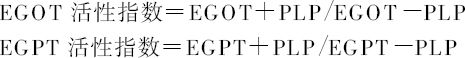
\includegraphics[width=5.95833in,height=4.26042in]{./images/Image00012.jpg}
\end{table}

近年来,机会致病菌性肺炎有增多的趋势。机会感染的致病条件为全身防御能力的严重降低,其诱因为:①基础疾病如恶性肿瘤,肝、肾衰竭,呼吸衰竭,糖尿病,大面积烧伤,白血病,器官移植后免疫抑制剂的应用,遗传性或获得性免疫缺陷综合征(AIDS)等;②附加因素如长期静脉(或膀胱)留置导管,气管插管,长期使用广谱抗菌药物致正常菌群失调,药物或放疗所致白细胞减少或反应性改变,以及T和(或)B淋巴细胞介导的免疫功能降低等。机会致病菌性肺炎有易感性、难治性和反复性等特点,临床症状多不典型,特别在糖皮质激素治疗中可无明显的发热和感染中毒症状。虽用抗生素积极治疗,但常迁延不愈,并发症多。目前革兰氏阴性杆菌已成为医院内机会致病菌性肺炎的重要病原,此外还有嗜肺军团杆菌、非典型分枝杆菌、肺孢子菌、巨细胞病毒、念珠菌、曲霉、隐球菌等致病微生物,经常威胁着患者的生命健康。

\subsection{3.1 感染性疾病}

\subsubsection{3.1.1 病毒性感染}

\paragraph{一、流感病毒性肺炎}

流感病毒性肺炎一般发生于流感流行高峰期间。患者除有流感本身的症状外,发病早期即有呼吸困难甚或发绀。肺部体征为叩诊轻浊音以及由两侧肺底向上蔓延的湿性啰音等。X线检查主要表现为间质性肺炎,并夹杂以不同形态的支气管肺炎样改变,可见肺内斑片状、多叶段渗出性病灶;进展迅速者,可发展为双肺弥漫的渗出性病变或实变,个别病例可见胸腔积液。季节性甲型流感(H1N1、H2N2和H3N2等)所致的病毒性肺炎主要发生于婴幼儿、老年人、慢性心肺疾病及免疫功能低下者,2009年甲型H1N1流感还可在青壮年、肥胖人群、有慢性基础疾病者和妊娠妇女等人群中引起严重的病毒性肺炎,部分发生难治性低氧血症。

流感病毒性肺炎的诊断根据是:①病例发生于流感流行期间,起病较急,在发病早期伴有显著的呼吸系统症状,如咽痛、流涕、咳嗽、呼吸困难,肺部可有啰音等;②血象白细胞数正常或减少;③X线检查肺部有肺炎征象,主要呈支气管肺炎和间质性肺炎表现,也可有肺实变表现;④曾用抗菌药物治疗而未见良效者;⑤鼻咽分泌物或口腔含漱液可分离出流感病毒或病毒抗原、核酸检测阳性。恢复期血清中抗流感病毒抗体滴度比急性期有4倍或以上升高有助于回顾性诊断。

流感病毒性肺炎主要须与肺炎支原体肺炎、肺结核等相区别。

\paragraph{二、高致病性人禽流感病毒性肺炎}

禽流感(禽流行性感冒)是禽类的甲型流感病毒亚型感染。1997年香港特别行政区出现人群暴发禽流感H5N1病毒感染,18例患者中6例死亡,是全球首次发现禽流感病毒能够直接感染人类。目前发现且证实可感染禽类又可感染人类的主要为禽甲型流感病毒H5N1、H9N2、H7N7和H7N9亚型,其中以H5N1亚型引起的病情重,病死率高。2013年3月底华东地区发现的H7N9禽流感病毒是全球首次发现的新亚型流感病毒,至2013年9月底我国内地共报告134例人感染H7N9禽流感确诊病例,其中死亡45人。人禽流感的传染源主要为患禽流感或携带禽流感病毒的鸡、鸭、鹅等家禽,特别是鸡;传播途径主要通过呼吸道,目前尚无人与人之间传播的确切证据。高危人群为与不明原因病死家禽或感染、疑似感染禽流感家禽密切接触人员。人禽流感的潜伏期一般为1~3天,通常在7天以内。临床上多为急性起病,早期表现流感样症状,主要为发热,体温大多持续在39℃以上,热程1~7天,一般为3~4天,可伴有流涕、鼻塞、咳嗽、咽痛、头痛和全身不适。部分患者可有恶心、腹痛、腹泻、稀水样便等消化道症状。重症患者病情发展迅速,可出现肺炎、急性呼吸窘迫综合征、肺出血、胸腔积液、全血细胞减少、肾衰竭、败血症、休克及雷氏(Reye)综合征等多种并发症。体检时重症患者有肺部实变体征。实验室检查外周血白细胞总数一般不高或降低,重症患者多有白细胞总数及淋巴细胞下降。重症患者胸部X线检查可显示单侧或双侧肺炎,少数可伴有胸腔积液等。其影像学特征有:①胸部X线主要表现为肺实质渗出性病变,两肺可见大片状及团絮状高密度影,中心区密度较高,边缘区密度较淡。阴影密度高于常见的病毒性肺炎;②影像学改变变化快,呈游走性;③典型病变病灶累及两肺,大致呈对称性,分布广泛;④临床症状与胸部X线表现不完全相符。病灶吸收落后于临床。诊断依靠流行病学史,结合临床表现和实验室检查,并排除流感、普通感冒、细菌性肺炎、严重急性呼吸综合征(SARS)、传染性单核细胞增多症、巨细胞病毒感染、衣原体肺炎、支原体肺炎等疾病后,可作出临床诊断。确诊有赖于病原学及血清学检测结果,最可靠的方法是从呼吸道标本中分离出禽流感病毒亚型。

\paragraph{三、严重急性呼吸综合征}

严重急性呼吸综合征(SARS)是新出现的传染病是由SARS冠状病毒所致的一种具有明显传染性、可累及多个脏器系统的特殊肺炎。主要通过飞沫、气溶胶或接触污染的物品传播。

潜伏期为2~10日,起病急骤,多以发热为首发症状,体温常>38℃,可有寒战、咳嗽、少痰,偶有血丝痰,心悸、气促,甚或呼吸窘迫。可伴有肌肉酸痛、头痛、关节痛、乏力和腹泻。患者多无上呼吸道卡他症状。肺部体征不明显,部分患者可闻及少许湿啰音,或有肺实变体征。抗菌药物治疗无效。患者的呼吸道症状和肺部体征与胸部X线检查的改变相比常常较轻。实验室检查外周血白细胞计数一般不升高或降低,淋巴细胞减少。胸部X线早期可无异常表现或淡薄阴影,随疾病发展可见不同程度片状、斑片状浸润阴影,或呈网状样改变;部分患者肺部病变进展迅速,呈大片浓密模糊炎性浸润阴影,边缘不清,分布在一个或数个肺叶(段),多为双侧改变,严重者呈“白肺”。肺部阴影吸收消散较慢,与临床体征可不一致。

诊断上强调流行病学史,疑似者可做血清SARS冠状病毒的特异抗体检测和鼻冲洗液或含漱液PCR检测,注意排除上感、流感、细菌性或真菌性肺炎、艾滋病合并肺部感染、军团菌病、肺结核、流行性出血热、肺部肿瘤、非感染性间质性疾病、肺水肿、肺不张、肺栓塞、肺嗜酸性粒细胞浸润症、肺血管炎等临床表现类似的呼吸系统疾病。

\paragraph{四、艾滋病}

艾滋病(AIDS)合并肺部病变引起发热并非少见。有作者提出有下列情况2项或以上者须考虑AIDS肺部病变:①双侧肺门周围网状或网结状阴影;②上述改变在3~5日迅速发展为两肺弥漫性肺间质肺实质浸润甚至为均质性肺实变;③结节样、线条样病变,伴有或不伴有肺门或纵隔淋巴结肿大;④肺部炎症经积极治疗无效甚至病灶发展增多。

如患者同时有下列1项危险因素伴1项相关症状时,即检测抗HIV抗体帮助诊断。

危险因素:①有静脉药瘾史;②有同性恋或异性乱交史;③10年内有输血或输血制品史;④来自流行地区曾与AIDS可疑患者接触史。

相关症状:①长期发热(>1个月)伴体重减轻;②慢性腹泻>1个月;③咳嗽1个月以上,伴气短;④剧烈头痛,甚至出现脑膜刺激征。

AIDS肺部感染的病原体主要有肺孢子菌,此外,巨细胞病毒、弓形虫、隐球菌、类圆线虫、军团菌、肺结核、非结核分枝杆菌等也可引起肺炎,请参阅有关章节。

\paragraph{五、巨细胞病毒肺炎}

巨细胞病毒(CMV)肺炎多发生在免疫抑制宿主,如恶性肿瘤、接受大量免疫抑制剂、细胞毒药物、放射治疗、AIDS等免疫功能低下者易罹患本病。近年器官移植病例增多,特别是肾移植、骨髓移植术后常发生严重的CMV感染,病死率高。如有以下情况,应高度怀疑巨细胞病毒肺炎:①免疫抑制宿主,器官移植受者多发生在术后2~4个月;②发热,体温多在38℃以上;③阵发性干咳,常伴有明显的呼吸困难;④多有全身症状,关节肌肉疼痛、腹胀、直立性低血压等;⑤肺部体征无明显异常;⑥X线胸片早期可能无异常发现,随病情发展逐渐出现双侧弥漫性间质性肺炎或肺泡浸润,肺外周和肺底部常被累及。

确诊需借助实验室检查,常用的检查包括病毒分离、PCR、核酸杂交、抗原血症、DNA血症、mRNA血症等。

\paragraph{六、腮腺炎病毒性肺炎}

国内报告一组成年人流行性腮腺炎并发肺炎的主要表现是临床症状与体征均不显著,仅少数有微热、咳痰或全身不适等症状。胸部X线检查发现肺野内散布有点状、小斑片状或大片状不均匀密度的阴影,通常以右下肺野较为显著,持续时间较长,为48~165天(平均95.7天)。血象无特殊改变。冷凝集试验阴性。磺胺类药物、青霉素、氯霉素治疗均不能使肺部X线征改善。肺部病变大概由于腮腺炎病毒侵犯肺间质及肺泡壁所致。

\paragraph{七、肺炎型传染性单核细胞增多症}

临床症状以发冷、发热、疲乏、淋巴结肿大、咽充血、肌酸痛、头痛、纳差等最为常见。肺炎的表现主要为咳嗽、胸痛,部分病例有血丝痰或铁锈色痰。体检仅1/3病例有肺实变征,但X线检查所有病例均有显著改变。X线胸片所见可分为斑片状、磨玻璃状、堆云状肺部阴影或肺纹理增多,其中以磨玻璃状阴影最具特征性。斑片状阴影与肺炎支原体肺炎所见者相似。病例都有传染性单核细胞增多症的血象,均呈阳性嗜异性凝集反应,经豚鼠肾吸收后,效价在1∶64~1∶2048之间。

此病主要须与肺炎支原体肺炎相区别,二者的X线征可有相似之处,且均可有阳性的嗜异性凝集反应与冷凝集反应,偶尔在传染性单核细胞增多症时,冷凝集试验效价可相当高,故阳性嗜异性凝集反应须经豚鼠肾吸附试验证实或(及)作冷凝集素类型测定,方有鉴别诊断意义。

此外,传染性单核细胞增多症时,血象多有大量的异形淋巴细胞出现,而在肺炎支原体肺炎则无此现象;前者对四环素类抗生素治疗的疗效不确定,也与肺炎支原体肺炎有所不同。表\ref{tab2-9}可作为二者鉴别的参考。
%\begin{table}[htbp]
%\centering
%\caption{肺炎型传染性单核细胞增多症与肺炎支原体肺炎的鉴别}
%\label{tab2-9}
%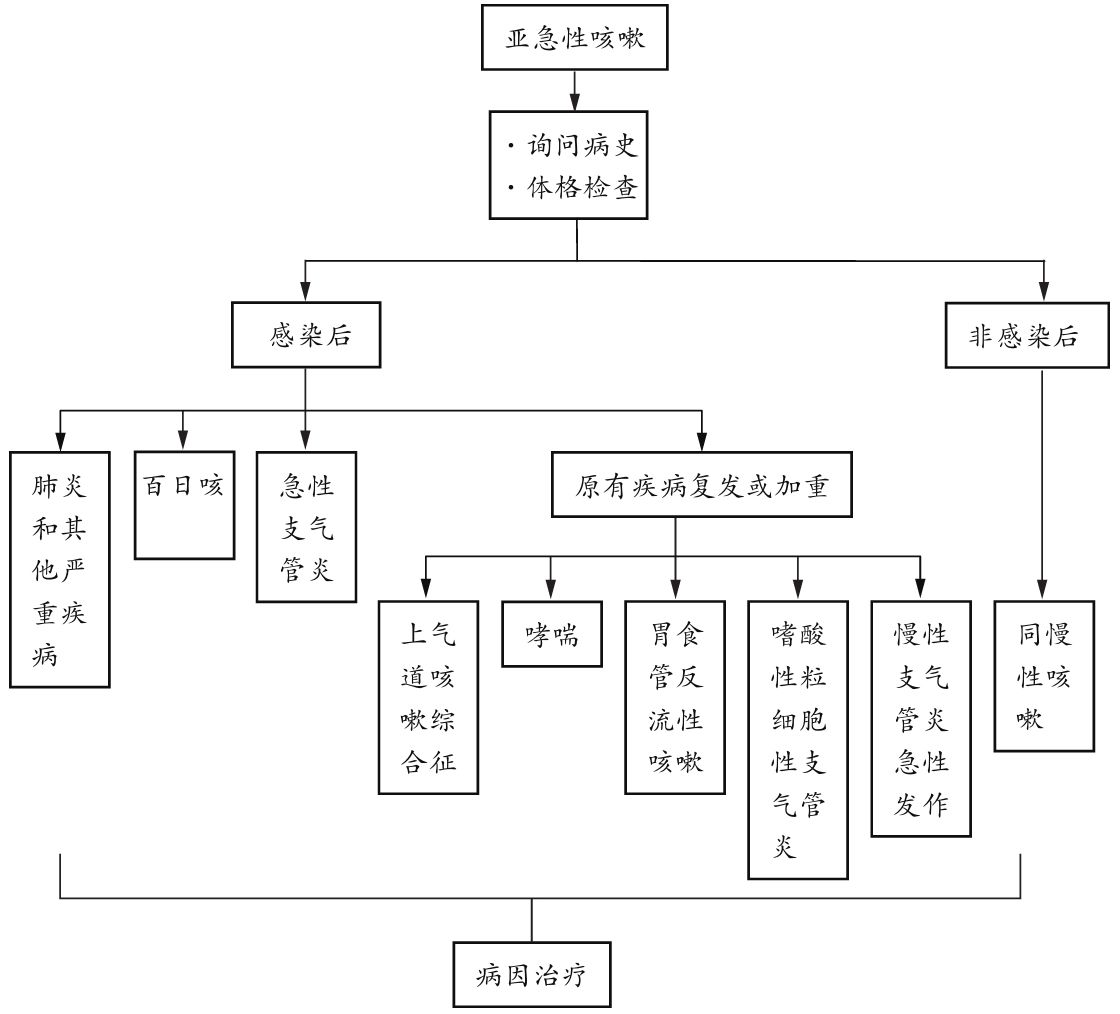
\includegraphics[width=5.96875in,height=2.25in]{./images/Image00013.jpg}
%\end{table}
%续表
%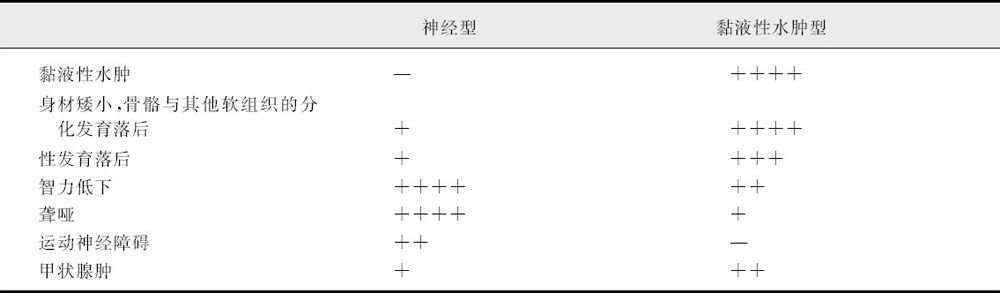
\includegraphics[width=5.90625in,height=1.33333in]{./images/Image00014.jpg}

\begin{longtable}{c}
  \caption{肺炎型传染性单核细胞增多症与肺炎支原体肺炎的鉴别}
  \label{tab2-9}
  \endfirsthead
  \caption[]{肺炎型传染性单核细胞增多症与肺炎支原体肺炎的鉴别}
  \endhead
  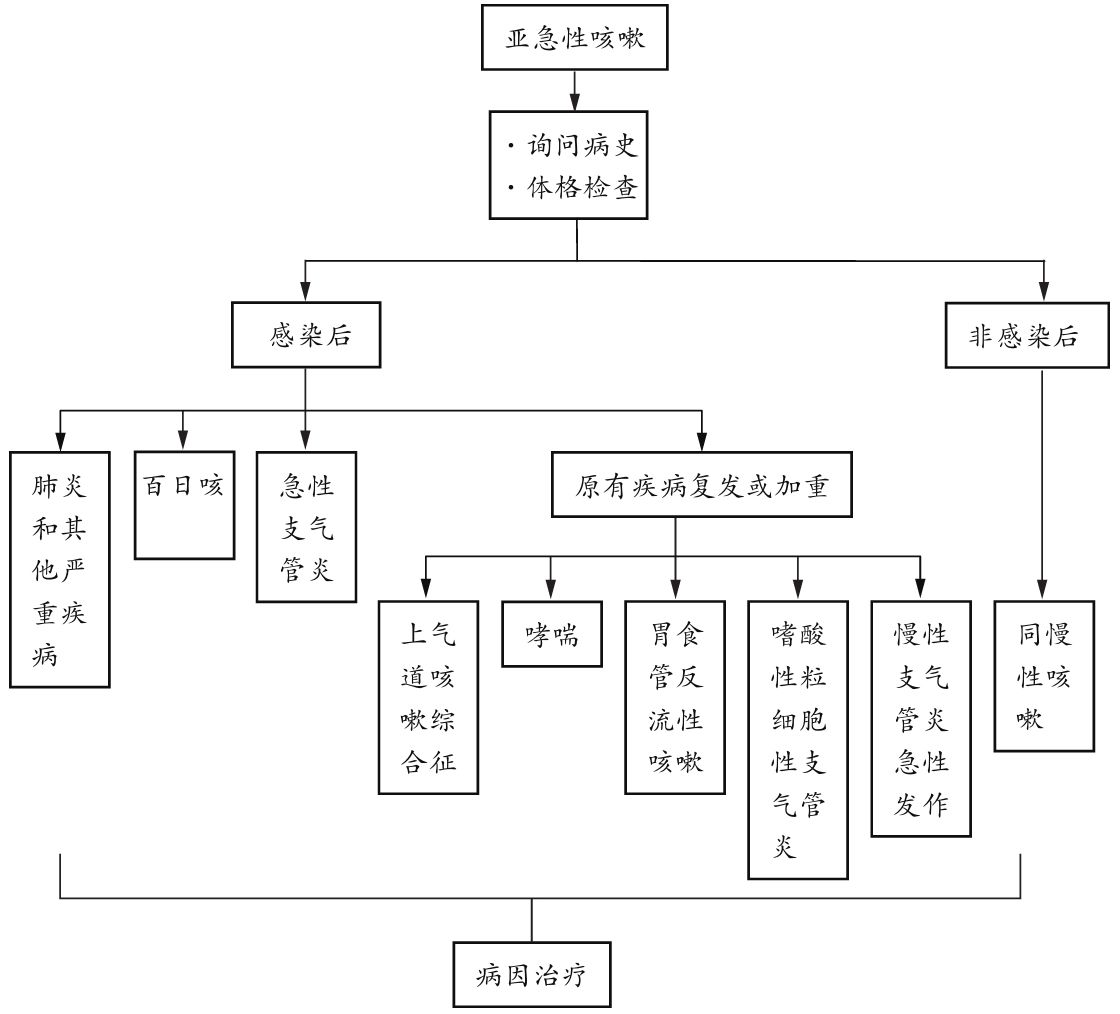
\includegraphics[width=\textwidth,height=\textheight,keepaspectratio]{./images/Image00013.jpg} \\
  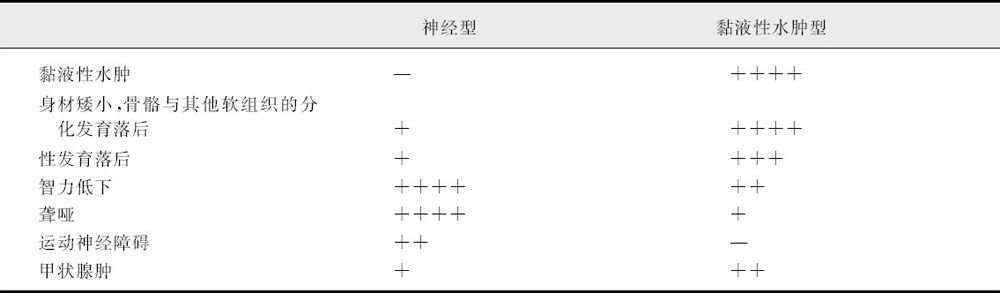
\includegraphics[width=\textwidth,height=\textheight,keepaspectratio]{./images/Image00014.jpg} \\
\end{longtable}

\subsubsection{3.1.2 细菌性感染}

细菌性肺炎的病原体因患病环境不同而有差异。社区获得性肺炎以肺炎链球菌、流感嗜血杆菌、卡他莫拉菌以及非典型病原体常见。医院获得性肺炎除了以上细菌外,还有金黄色葡萄球菌、铜绿假单胞菌、肠杆菌属和肺炎克雷伯杆菌等。病原体可通过空气吸入、血流播散、邻近感染部位蔓延、上呼吸道定植菌误吸、胃肠道反流物误吸和通过人工气道吸入环境中的致病菌引起。细菌性肺炎常以恶寒或寒战、高热起病,呼吸道症状较重,血白细胞增多常在15.0×
10\textsuperscript{9}
/L以上(肺结核可例外),分类以中性粒细胞占优势,并有明显的核左移与中毒性颗粒。血C-反应蛋白和降钙素原升高。

\paragraph{一、肺炎链球菌肺炎}

发病多见于冬春季节,青壮年男性罹患较多。发病前常有受凉、淋雨、饥饿、疲劳、醉酒病毒感染史。起病急骤,多以寒战突然起病,继而高热,多呈稽留热型。颜面潮红,呼吸浅速,甚至出现呼吸困难与发绀。患侧胸痛常见。咳嗽频繁,初为干咳,2~3天后咳出少量黏稠痰液,常呈铁锈色,以后逐渐变为脓性。可有唇疱疹出现。肺部病变部位常可发现轻浊音与捻发音。血象早期呈现白细胞增多、显著核左移与中毒性颗粒。

在病期第3~4天病变侵及整个肺叶,出现明显肺实变体征,浊音界与受累肺叶的境界相一致,听诊发现支气管呼吸音、细湿啰音与捻发音,此时临床诊断更为明确。

肺炎链球菌肺炎早期无特征性表现,凡患者突然畏寒或寒战、高热、胸痛伴肺部呼吸音减弱,白细胞增多,须考虑此病的可能性。胸部X线检查对早期诊断最有帮助。在发病后24~36小时作X线检查,受累肺叶可见有阴影出现,而此时体检可尚无典型的实变体征。此阴影通常从肺门向外周扩展,最后侵及整个肺叶,但目前典型的大叶性病变不多见。痰液涂片染色镜检及培养可证明肺炎链球菌的存在。尿肺炎链球菌抗原可阳性。

近年国内报道的重症肺炎,患者以中、老年人较多,但青壮年者也不少。患者的主要临床表现为高热或体温不升,呼吸困难,明显发绀,白细胞增多或减少,但核左移显著。重症肺炎有时局部体征不明显,甚至有时须经尸检才能证实诊断。

有的病例早期出现意识不清、谵妄、抽搐、昏迷、脑膜刺激征等症状,而肺炎体征尚未显露,易误诊为败血症、流脑、脑炎等疾病。个别病例表现为发热、腹痛、黄疸,可误诊为急性胆囊炎。个别右下叶肺炎患者呈右下腹痛,可误诊为急性阑尾炎。因此凡在肺炎多发的冬春季节,遇见原因未明的急性发热兼有上述表现者,切勿忽略肺炎的可能性,如病情许可应及时做X线检查以明确诊断。

\paragraph{二、肺炎克雷伯杆菌肺炎}

临床特点类似肺炎链球菌肺炎。国内报道的一组病例中,患者都为中年与老年男性,多发于慢性消耗性疾病与免疫力低下的基础上,如原有肺部疾病、糖尿病、手术后和酒精中毒的患者。此病发病急骤,以寒战、高热起病,并有胸痛、呼吸困难与发绀,患者呈急性重病容。神经精神症状也常见。重症病例可迅速发生休克而危及生命。痰为砖红色、血样,或胶冻样类似杨梅果酱,甚黏稠,但也可呈铁锈色。痰中可发现大量肺炎克雷伯杆菌。血象常呈中等度白细胞增多,核左移。肺实变体征可能早期出现,但无典型体征者较常见,甚至X线照片上显示大片致密阴影时,体检仅发现轻浊音和不明显的支气管呼吸音。主要并发症有脓胸、气胸、败血症和慢性肺炎等。

X线检查病变包括大叶实变、小叶浸润和蜂窝状脓肿(坏死性肺炎)形成。大叶实变多位于右上叶,重而黏稠的炎性渗出物使叶间裂呈弧形下坠。免疫功能抑制和慢性肺部疾患者表现为小叶浸润。16\%~50\%伴脓肿形成,形成单个或多个薄壁脓肿,最后遗留广泛性纤维性变或变为迁延性慢性肺脓肿。

临床上遇见年纪较大、全身情况较差的急性肺炎患者,痰中发现较多的疑似肺炎克雷伯杆菌时,应提高警惕。特别是在青霉素治疗下未见好转,肺部病变反而进展时,或在病程中迅速发生休克时,应立即作痰涂片及培养检查。

\paragraph{三、金黄色葡萄球菌性肺炎}

金黄色葡萄球菌引起的急性化脓性炎症。常发生于有基础疾病如糖尿病、血液病、艾滋病、肝病或原有支气管肺疾病者。儿童患流感或麻疹时亦易罹患。年老、体弱、较长期应用广谱抗生素或糖皮质激素等均为发病诱因。

多急骤起病,高热、寒战,发热多呈不规则型或弛张型,胸痛,痰脓性,可早期出现循环衰竭。此病与肺炎链球菌肺炎在临床上的不同点是:败血性经过,热程较长(2~4周),治疗显效后徐缓解热。特征性痰呈脓血性或黏液脓性,与肺炎链球菌肺炎的铁锈色痰有所不同。约半数病例出现皮疹,可为荨麻疹、出血性斑丘疹、瘀斑或瘀点等,而无唇疱疹出现。胸部体征早期不显著,仅呈轻浊音、呼吸音减弱及细湿啰音。胸部体征往往与严重的呼吸困难、发绀、血性痰、休克等症状不相称。

血白细胞增高,中性粒细胞比例增加,核左移并有中毒颗粒。此病的X线特点是:多发性小叶性炎症浸润阴影,但也可为大叶性,病灶内空洞形成、蜂窝状改变或肺气囊肿的出现等,其中尤以后者对诊断更有价值。痰、胸腔积液或血培养的阳性结果,有助于本病的确诊。

临床上如患者有下列表现之一时,须考虑金黄色葡萄球菌性肺炎的可能性:①恶寒或寒战、发热,咳嗽,胸痛,气促,咳脓血痰及伴有皮疹者;②败血症或流感后出现与胸部体征不相称的呼吸困难、发绀等症状,发热迁延不退或退热后又复燃者;③短期内两肺多发性炎症病灶,或一侧肺炎早期即出现肺脓肿、胸膜炎或肺气囊肿者;④已诊断为肺炎,但对青霉素治疗无良好反应者。遇此情况应做细菌学检查,同时加强抗菌药物的应用。

\paragraph{四、铜绿假单胞菌肺炎}

铜绿假单胞菌是医院获得性肺炎的常见病原体,它容易定植于呼吸道,广谱抗菌药物的使用会增加其定植风险。有文献报道4\%~15\%COPD患者痰中可分离到该菌。其近年来发病率呈上升趋势,且由于铜绿假单胞菌极易耐药,并不易为呼吸防御机制杀灭,治疗困难,病死率高。细菌的入侵途径通常是上呼吸道、皮肤与消化道。由于大面积皮肤烧伤合并铜绿假单胞菌感染而引起肺炎者也有时可见。高龄、体弱、原有慢性心、肺疾病、应用广谱抗生素以及器械污染等,是常见的发病诱因。

此病临床上除急性肺炎表现外,往往早期出现谵妄、发绀,并有倒错性发热(即热峰在每天上午出现)及相对缓脉。咳嗽时伴黄脓性痰,少数患者咳出的痰呈浅绿色。重症者可有低血压或休克。胸痛和咯血不常见。肺部X线征是双下肺广泛支气管炎性肺炎,伴有结节状阴影及多发性小脓肿形成,肺脓肿发生较早。

此病经过较重,预后凶险。血流感染发生率低,多见于免疫抑制宿主,因此确诊有赖于痰或胸腔积液的细菌培养。

\paragraph{五、支气管扩张并发感染}

支气管扩张并发急性细菌感染时,患者有发热、咳嗽、咳脓痰等症状,或咯血后出现感染的症状。X线胸片所见类似支气管肺炎、干酪样肺炎或浸润型肺结核。诊断须根据既往病史与治疗效果。如过去屡次在同一部位发生肺炎,则强烈支持支气管扩张合并感染的诊断。此病经积极的抗菌治疗后,往往迅速得到控制,大片阴影逐渐消失,成为索条状卷发阴影。有些感染经治不愈,要考虑是否合并非典型分枝杆菌感染、结核感染等。

\paragraph{六、急性肺脓肿}

急性肺脓肿根据感染途径可分成三个类型:

\subparagraph{(一)吸入性肺脓肿}

大多数肺脓肿主要由于吸入上呼吸道或口腔内带有细菌的分泌物所引起。全身衰弱、受凉、醉酒、中毒、鼻窦炎等常为发病基础。麻醉与手术、食物反流或呕吐、昏迷状态、溺水等均可为诱因,而睡眠中吸入感染则被认为是最常见的诱因。致病菌多为厌氧菌,其他常见菌有化脓性链球菌、金黄色葡萄球菌、肺炎克雷伯杆菌和铜绿假单胞菌等,但往往是多种细菌的混合感染。

患者往往以恶寒或寒战、高热、虚弱、胸痛、心率加快等症状急骤起病。体温常呈弛张热、稽留热或不规则型热。患者大多无呼吸困难与发绀。胸部体征常不显著,但也可呈轻浊音、呼吸音减弱或粗糙、散在性湿啰音等。白细胞显著增多与核左移。只根据胸部体格检查,易忽略肺脓肿的诊断,尤其是深在的肺脓肿往往无明显的体征。炎症浸润破溃后形成脓肿,脓肿向支气管穿破时患者突然咳出大量脓臭痰及坏死组织,静置后多可分为三层:上层为泡沫样痰,中层为黏液样成分,下层为坏死组织。

脓肿分布多位于右肺,右上肺的后段最常累及,其次为左、右下肺叶的背段。X线检查早期可见肺野有单个或多个界限模糊的片状阴影。嗣后此阴影的中心变为圆形透亮区,出现气液平面,转换体位时此气液平面随之改变,据此可以确定肺脓肿的诊断。

\subparagraph{(二)继发性肺脓肿}

某些细菌性肺炎(金黄色葡萄球菌、铜绿假单胞菌和肺炎克雷伯杆菌等)、支气管扩张、支气管囊肿、支气管肺癌、肺结核空洞等继发感染可导致继发性肺脓肿。支气管异物阻塞,也是导致肺脓肿特别是小儿肺脓肿的重要因素。肺部邻近器官的化脓性病变,如膈下脓肿、肾周脓肿、脊柱旁脓肿或食管穿孔等波及到肺也可引起肺脓肿。阿米巴肝脓肿好发于右肝顶部,易穿破膈肌至右肺下叶,形成阿米巴肺脓肿。

\subparagraph{(三)血源性肺脓肿}

通常并发于败血症,特别是金黄色葡萄球菌败血症的病程中。细菌性栓子血行播散到肺,引起小血管栓塞、炎症和坏死而形成肺脓肿。脓肿常为多发性,且常为双侧性。患者在全身感染的基础上发病,常伴高热、寒战、胸痛、咳嗽及血痰。痰量不多,肺部体征不明显。诊断主要依靠X线检查。胸部平片显示双肺多发性圆形病灶。脓肿形成后可见气液平面,有的形成张力性脓腔,可破裂而发生脓气胸。血培养常有致病菌生长,提示脓肿发生在败血症的基础上。也应细致检查其他器官的迁徙性化脓病灶。

\paragraph{七、肺结核}

血行播散型肺结核、浸润性肺结核、空洞性肺结核、干酪样肺炎、结核性胸膜炎等都可引起急性发热与肺部病征,临床上须与其他原因的肺部病变相区别。

\subparagraph{(一)血行播散型肺结核}

亦称急性粟粒型肺结核,多见于婴幼儿和青少年,特别是营养不良、患传染病和长期应用免疫抑制剂导致抵抗力明显下降的小儿,也可见于成人。起病急,持续高热,中毒症状严重。虽然病变侵及两肺,极少有呼吸困难,但也有发生急性呼吸窘迫综合征者。可有全身浅表淋巴结肿大,肝脾大,有时可发现皮肤淡红色粟粒疹和脑膜刺激征。体检时肺部叩诊与听诊体征轻微或缺如,与病情的严重性不相称,如不注意常易致误诊。X线胸片和胸部CT可见由肺尖至肺底呈大小、密度和分布三均匀的粟粒状结节阴影,结节直径2mm左右。参见第28节。

\subparagraph{(二)浸润性肺结核}

属于继发型肺结核,由新发的吸入感染,或由局限性病灶、播散性病灶恶化而成,为活动性肺结核。罹患者多在20~30岁。轻者无明显症状,有些患者呈急性发热,与流行性感冒的临床表现相似,其他为长期微热、心悸、盗汗、乏力、容易烦躁、微咳、咳痰、厌食、体重减轻等中毒症状。

肺部体征因病灶大小、数量及部位而定。病灶小者无异常体征。病灶较大或较多时,可出现轻浊音与细湿啰音(多在锁骨下窝部位)。血沉中等度增速。痰中常可检出结核杆菌。

X线检查显示下列特点:病变部位不定,在成年人多发生在肺尖、锁骨下部;病变多样性,阴影密度较浅,如絮状,边缘模糊,界限不清,可融合和形成空洞。

鉴别诊断上须与肺炎支原体肺炎、不完全性大叶性肺炎、肺吸虫病、支气管扩张合并感染等相区别。

下肺结核 下肺结核临床上少见,可见于艾滋病、糖尿病和其他免疫抑制患者的肺结核,病变位于肺门以下,发病右下叶多于左下叶。咯血是常有的症状;全身中毒症状与一般上肺结核无差异,但病程发展较快。发病常类似支气管肺炎。X线阴影特征与一般肺结核相同,但以大片状广泛浸润为多,且在早期即可有肺不张与空洞形成。早期诊断往往较为困难,最易误诊为肺脓肿与肺炎,有时甚至被误诊为肺包虫病。下列几点有助于早期鉴别诊断:

1.下肺结核患者有恶寒、寒战者少见。咳嗽与胸痛一般较肺炎或肺脓肿为轻,脓痰不多见,病程则较肺炎或肺脓肿为长。

2.大多数下肺结核患者的白细胞总数在正常范围内。

3.肺脓肿与下肺结核好发部位虽然都在肺下叶背段,但青年患者在下叶背段有空洞性病变,而症状与肺脓肿不尽相符时,应注意下肺结核的可能性。

4.下肺结核诊断的主要根据是痰中查得结核杆菌,应反复进行痰集菌涂片检查,必要时作培养或动物接种。

5.相当数量的下肺结核患者同时有支气管内膜结核,支气管镜检查是诊断的重要方法之一。

\subparagraph{(三)空洞性肺结核}

亦属于继发性型肺结核,临床症状较多,发热,咳嗽,咳痰和咯血等。空洞形态不一,可呈虫蚀样空洞、薄壁空洞、厚壁空洞、张力性空洞以及干酪溶解性空洞等,多有支气管播散病变。空洞内一般无气液平面,空洞周围炎性病变较少,常伴有条索、斑点及结节状病灶。痰中一般容易检到结核杆菌。合并肺炎时,应与肺脓肿相鉴别。

\subparagraph{(四)干酪样肺炎}

亦属于继发型肺结核,与浸润性肺结核不同,主要是干酪样变化比病灶周围炎变化显著,进展急剧,是严重的结核病类型。干酪样肺炎起于结核杆菌的支气管播散,在机体抵抗力极度降低和对结核杆菌过敏反应增高的情况下发病,临床与病理上可区分为大叶性干酪样肺炎与小叶性干酪样肺炎两种:

\hypertarget{text00025.htmlux5cux23CHP2-7-1-2-7-4-1}{}
1.大叶性干酪样肺炎

发病急,与肺炎链球菌肺炎相似,但温度上升较慢,经2~3天升至39~40℃,逐渐转为弛张热,并有恶寒、呼吸困难、胸痛、咳嗽、咳痰、痰中时有带血、纳差、极度疲乏等症状。体检可发现呈大叶分布的肺实变体征。X线检查发现大片阴影,数周后可溶解形成空洞,呈虫蚀样空洞。血象白细胞计数正常或轻度增多。大部分于发病一个月左右痰中发现结核杆菌。此病主要须与非结核性大叶性肺炎(主要是肺炎链球菌大叶性肺炎)相鉴别。干酪样肺炎发病较后者为慢,无唇疱疹,无铁锈色痰,颜面苍白而非潮红,痰中可找到结核杆菌,血中白细胞数通常在15.0×10\textsuperscript{9}
/L以下,对青霉素疗效不佳,且患者发病前往往已有食欲欠佳、消瘦、潮热、盗汗等结核全身中毒症状。由于此病经过严重,凡遇到大叶性肺炎而疑为结核性时,应即积极进行抗结核治疗,以免耽误病情。干酪样肺炎兼有空洞时须与肺脓肿相鉴别,前者有空洞形成时痰中应找到结核杆菌。

\hypertarget{text00025.htmlux5cux23CHP2-7-1-2-7-4-2}{}
2.小叶性干酪样肺炎

多见于病程长、治疗效果不佳、全身情况及抵抗力很差的慢性肺结核患者,或发生于并发糖尿病的肺结核患者,主要病变是散布于两肺的多数性干酪样病灶。这些病灶可同时或分批出现。X线胸片上显示大小不一、边缘模糊的阴影.可能为3~5片至7~8片不等。上述情况的患者如突然发生急性肺部感染的症状,如畏寒、发热、咳嗽、咳痰、脉快、呼吸困难、发绀等时,应考虑小叶性干酪样肺炎的可能性。体检可发现两肺散在性干性与湿性啰音,但叩诊浊音不显著。小叶性干酪样肺炎早期与非结核性小叶性肺炎不易鉴别,主要鉴别根据为前者血中常无白细胞增多,或仅轻度增多,而后者常有明显的白细胞增多;前者痰中常可找到结核杆菌而后者则无。

\paragraph{八、军团菌肺炎}

本病首次在美国(1976年)发现,近年国内多处亦发现有散发病例,还曾有暴发性流行。潜伏期2~10天。临床表现为倦怠、头痛、肌痛、发热(可达40℃或以上)和相对缓脉等,可有畏寒或寒战,或不同程度的消化道症状与精神神经症状。咳嗽逐渐出现并加剧,伴胸痛与咳黏液痰,痰数日后转为脓性。突出的血生化改变为低钠血症与低磷血症。部分病例可合并肝功能损害。典型X线胸片为早期一侧肺下野出现境界不清的浸润阴影,多呈斑点状间质浸润或致密性实变。其后扩大至一侧肺下野乃至一侧肺野。部分病例可累及双肺。1/3~2/3病例有不同程度的胸腔积液。患者痰液、胸腔积液和气管吸出物中均可检出军团菌。血清特异性免疫学检查亦有助于诊断。尿军团菌抗原及呼吸道分泌物直接荧光抗体染色法有助于本病早期诊断,前者敏感性是80\%~90\%,特异性是98\%~100\%,检测时间小于1小时,但后者敏感性较低。聚合酶链式反应(PCR)也有助于诊断,血、尿标本的敏感性为75\%~82\%,特异性90\%~100\%。诊断上本病与其他社区获得性肺炎相比较,头痛、腹泻、肌酸激酶值升高、严重低钠(<130mmol/L)、肝功能异常、对β-内酰胺类抗生素不敏感在军团菌肺炎中多见。1998年温思罗普大学发表了温思罗普大学医院(WUH)标准,以便于区分军团菌肺炎和其他细菌感染的肺炎(表\ref{tab2-10}\footnote{≥10分=临床诊断;5~9分=疑诊;<5分=排除。例1是临床诊断,例2为疑诊,例3排除})。但回顾性分析发现该标准能较好的区分军团菌肺炎和其他细菌感染的肺炎,但假阳性率较高。如用大环内酯类及氟喹诺酮类等药物治疗有效也支持诊断。另外,治疗后临床症状好转而胸片仍进一步恶化也是本病的特点之一。Fiumefreddo等提出另一社区获得性军团菌肺炎的临床诊断评分,分别是发热、无痰、血钠降低、LDH升高、C-反应蛋白升高和血小板降低6个指标,每项1分共6分,分值越高军团菌病可能性越大,≥4应高度怀疑军团菌病,此评分与WHU标准相比更为简单易用。其他还有CBPIS军团菌病评分系统也可应用(Clinical
Infectious Diseases.2003;37:483-9)。

\begin{table}[htbp]
\centering
\caption{WUH军团菌病评分系统}
\label{tab2-10}
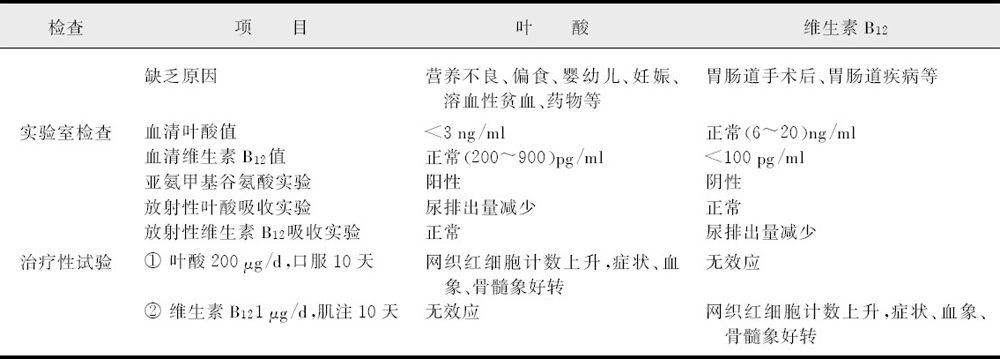
\includegraphics[width=6.03125in,height=6.58333in]{./images/Image00015.jpg}
\end{table}


据近年一组37例患者的综合分析,35\%有胃肠、肝、肾和神经精神异常的肺外症状,38\%有低钠血症,40\%合并胸腔积液,17\%合并肺脓肿。由此可见本病临床表现为全身性症状和呼吸系统症状。X线胸片肺部病变的恢复迟于临床改善,有些病例仍有进展。

\paragraph{九、肺型炭疽病}

诊断炭疽病须注意流行病学史。此病是重要职业病之一,主要见于从事畜牧、皮毛、毛织等职业的人,或曾与病畜接触的人。近年有用于生物恐怖活动。肺型炭疽病的发生是由于吸入混有炭疽杆菌芽胞的尘埃而致感染,又称“吸入性炭疽”,预后很差,但临床上少见。凡遇有急性发热患者伴有肺部感染症状,咳泡沫样血痰而兼有上述流行病学史者,须考虑有肺型炭疽病的可能性。

发病急骤,有寒战、高热、咳嗽、胸痛、大汗、心率增速、气促、喘鸣、发绀等症状,继而咳出锈色或血样痰。患者神志一般清醒。重症者发绀显著,血压下降,脉搏细速,有明显的休克现象。肺部体征仅可闻及散在的细湿啰音,或有胸腔积液征。体征与病情严重程度不成正比。血象白细胞数增高。

确诊须依靠细菌学检查。痰与胸腔渗出液直接涂片,均可发现革兰氏染色阳性、具有荚膜的粗大的炭疽杆菌。培养也容易获得阳性结果。

\hypertarget{text00025.htmlux5cux23CHP2-7-1-2-10}{}
十、肺型鼠疫

鼠疫是危害人类最严重的烈性传染病之一,病原体为鼠疫杆菌,传染源为受感染的鼠类或其他野生啮齿类动物。

鼠疫潜伏期多为2~3天,甚少超过5天。肺型鼠疫可分原发性与继发性两种。前者于发病后即出现肺部征象,表现为急性肺-胸膜炎;后者则继发于腺鼠疫之后。

肺型鼠疫发病急骤,患者有寒战、高热、胸痛、咳嗽、咳痰。痰最初为黏液性,后变稀薄稍带泡沫,不久可成为鲜红色血样,痰中含大量鼠疫杆菌。呼吸困难与发绀迅速出现。肺部体征多不明显,有时可发现肺部局限性浊音、散在性湿啰音与捻发音、胸膜摩擦音。X线检查可为正常或仅发现轻微病变,往往与病情的严重性不相称。肺型鼠疫常发展为败血症,未接受及时有效治疗者常于2~3日内死于心力衰竭、出血、休克,病死率高达70\%~100\%。

凡在鼠疫可能发生的地区和环境,遇有急性肺部感染患者,有明显的中毒症状、早期衰竭,或同时有淋巴结肿痛及出血现象,应考虑此病的可能性。痰液细菌学检查(包括涂片及培养)容易获得阳性结果,对确诊提供可靠依据。

\hypertarget{text00025.htmlux5cux23CHP2-7-1-2-11}{}
十一、类鼻疽肺病

类鼻疽是类鼻疽伯克霍尔德菌(类鼻疽假单胞菌)引起的人兽共患传染病,主要通过污染的水源、土壤经破损皮肤传染,或经污染的食物由消化道传染。其发病具有地域性分布,主要在热带和亚热带,属于地方性传染病,我国海南、广东、广西、福建、香港、台湾是多发地区。类鼻疽病多发于中年(22~66岁,平均47岁)男性,农民与渔民多见,大多有基础疾病,如糖尿病、继发型肺结核和类风湿关节炎等。畏寒、发热见于所有患者。急性肺部感染是类鼻疽病的最常见类型,约占70.5\%,可为轻症的肺炎至严重的坏死性肺炎。起病多急骤,恶寒或寒战、高热(多呈稽留热)、头痛、全身肌痛、胸痛、干咳或有咯血,呼吸困难、休克和败血症等,体检有局部皮肤脓肿、肝脾和淋巴结肿大,肺部体征少,可有湿啰音。大多患者血白细胞升高,中性粒细胞占优势。半数患者有肝功能损害,71\%血培养类鼻疽假单胞菌阳性。胸部X线大多数为肺上叶病变,有浸润病灶及(或)空洞,空洞多为单发,大小差异很大,少有液平,常可与肺炎、肺结核或其他慢性肉芽肿疾病混淆。确诊主要依靠病原菌分离及血清学检查。病原学标本可来自血液、脓肿液、痰液和尿液等,血清学检查则用标准类鼻疽伯克霍尔德菌诊断血清,类鼻疽特异性抗体可阳性。

\hypertarget{text00025.htmlux5cux23CHP2-7-1-2-12}{}
十二、肺型土拉菌病(兔热病)

土拉菌病一般发生在夏季,潜伏期通常为1周。起病急骤,体温迅速上升达39~40℃,伴全身乏力,畏寒,头痛,背痛,全身肌痛。病情发展时出现谵妄、昏睡、烦躁不安等急性全身中毒症状。患者体温升高持续2~5天,随之徐缓下降。细菌侵入部位的局部淋巴结首先有痛感,2天内皮肤呈现原发性病灶,多发于手或手指。开始呈红丘疹,继而发生脓疱,破溃后,形成中心性坏死,逐渐变成边缘较硬的溃疡。肿大的局部淋巴结,亦可破溃。病程一般持续3~4周,恢复缓慢,约需2~3个月或更长。伤寒型(全身型或胸膜肺型)的土拉菌病是一种小叶性肺炎,病程为迁延性(1~2个月或更长),有时痰中带血,有化脓的倾向。患者常有较轻的中毒症状,肺部体征不明显,无唇疱疹及显著的白细胞增多,但往往并发干性或渗出性胸膜炎。诊断依靠流行病学史及细菌血清学检查。

\subsubsection{3.1.3 衣原体感染}

衣原体是一种介于病毒、细菌和立克次体间的微生物,更近似于细菌,其大小约0.2~0.4μm。可引起肺炎的衣原体主要有肺炎衣原体(TWAR)和鹦鹉热衣原体两种,少数由沙眼衣原体引起。

\paragraph{一、肺炎衣原体肺炎}

肺炎衣原体可引起上呼吸道感染,如鼻窦炎、中耳炎和咽炎,也可引起下呼吸道感染,如支气管炎和肺炎。近年肺炎衣原体肺炎患病率有增高的趋势,多感染儿童和老年人,占社区获得性肺炎的6\%~19\%,国内近年报道一组665例社区获得性肺炎肺炎衣原体占6.6\%。起病多隐袭,早期表现为上呼吸道感染的症状,如声嘶、咽痛、发热等,症状通常较轻,数天或数周后患者上呼吸道症状减退,开始出现咳嗽,提示下呼吸道受累。其他症状有肌痛、头痛、不适和乏力。重症感染可有脓痰、呼吸困难等,多见于COPD和心力衰竭患者。可伴有肺外表现如中耳炎、结节性红斑、心内膜炎、关节炎、甲状腺炎、脑炎和吉兰-巴雷综合征等。X线胸片显示肺叶或肺段的浸润病灶,多见于下叶。

病原体分离培养、聚合酶链反应、血清学试验如微量免疫荧光(MIF)抗体试验和补体结合(CF)抗体试验等有助于确诊。本病需与病毒性肺炎、支原体肺炎、流行性感冒、肺结核、真菌感染等鉴别。

\paragraph{二、鹦鹉热衣原体肺炎}

鹦鹉热衣原体寄生于鹦鹉、鸽、鸡等100余种家禽和野生鸟类体内,主要感染禽类和低等哺乳类动物,人类并不常见。通常发生于与受感染鸟密切接触者,感染途径为通过呼吸道吸入疫鸟排泄物气溶胶所致。病原体吸入体内后首先进入肝脾的网状内皮细胞进行增殖,再经血路进入肺和其他器官,所以人类的鹦鹉热既可以是呼吸道感染,也可能是以呼吸道为主的全身感染。

起病多隐袭,病情轻者如流感样症状。重症肺炎者多有寒战、发热、体温逐渐升高,第1周内可达40℃以上,热程3~4周,伴乏力、头痛、关节肌肉疼痛,亦可有结膜炎、口腔炎、鼻出血或出现类似伤寒的玫瑰疹。1周左右才出现呼吸道症状,如咳嗽、少量咳痰或痰中带血,病变严重者可有呼吸困难及发绀。病程中尚可出现纳差、恶心、呕吐、腹痛、腹泻等消化道症状,心肌炎、心内膜炎及心包炎,亦可有嗜睡、谵妄、木僵、抽搐、意识不清等神经精神症状。体检肺部体征常较症状轻,病初可无明显体征,以后可有湿啰音,少数患者可有肺实变征或胸腔积液征。X线胸片显示早期从肺门向外放射的浸润病灶。病灶可融合呈叶性分布,以下叶多见。常有弥漫性支气管肺炎或间质性肺炎的X线表现。肺内病变吸收缓慢。

本病确诊须依靠衣原体分离培养及(或)特异性血清学检查。PCR诊断效果更佳。本病需与病毒性肺炎、支原体肺炎、流行性感冒、肺结核、真菌感染等鉴别。与肺炎衣原体肺炎的鉴别主要是后者通常无鸟类接触史,临床症状较轻,体温很少超过37.8℃,且很少累及呼吸道以外器官。微量免疫荧光(MIF)抗体试验可用于鉴别不同的衣原体。

\paragraph{三、沙眼衣原体肺炎}

沙眼衣原体包括15个血清型,引起人类沙眼、性病淋巴肉芽肿、包涵体性结膜炎、生殖道感染,以及新生儿肺炎。在极少数情况下,沙眼衣原体也引起免疫缺陷成人患者的呼吸道感染,甚至正常成人的社区获得性肺炎,病因不清。

沙眼衣原体新生儿肺炎主要见于2~12周新生儿及婴儿,通过感染的母亲产道时受感染。大多数无发热,起始症状通常是鼻炎、伴鼻腔黏液性分泌物和鼻塞。随后发展为断续的咳嗽,呼吸急促和肺部啰音,可伴有心肌炎和胸腔积液。肺部X线显示间质浸润。半数患儿可伴有急性包涵体性结膜炎。

\subsubsection{3.1.4 支原体感染}

支原体是介于细菌和病毒之间,能独立生存而不需要寄身于其他生物细胞的最小微生物,目前已知的支原体有80余种。

肺炎支原体肺炎

由肺炎支原体感染引起的肺炎称为肺炎支原体肺炎,此病秋冬季节多见,但季节性差异并不明显。青壮年较易罹患。国内调查占社区获得性肺炎的20.7\%,且多合并其他细菌感染。潜伏期1~2周,缓慢起病,发热呈中等度,多持续约1~2周,也可持续3周。咽痛与咳嗽是常见的症状,发病初期以阵发性干呛性咳嗽为主,以后约半数病例可咳少量黏液痰或痰中带血丝,或小量咯血,而无铁锈色痰。这种呛咳和痰的特征是大叶性肺炎所少见。全身症状较为明显,如乏力、头痛、咽痛、纳差、腹泻、肌痛、耳痛等。体格检查肺部体征与X线征不相称,虽X线检查有显著的改变,但肺部实变征象却不明显。

血象白细胞总数多数正常,分类可呈相对性淋巴细胞增多与轻度或中等度嗜酸性粒细胞增多,这与细菌性肺炎的鉴别有一定意义。血清冷凝集反应阳性率高达80\%,效价达1∶32或以上有诊断价值,于病程第2~3周阳性率较高。血清支原体IgM抗体≥1∶64,或恢复期抗体滴度有4倍升高,可进一步确诊。直接检测呼吸道标本中肺炎支原体抗原,可早期快速诊断。

X线检查肺部阴影往往在发病后2~5天出现,通常有下列三项特点:①肺纹理增多;②沿增多的肺纹理出现不规则的斑片状实质阴影;③多数改变集中于肺门附近。病变所在以下叶为多。上述的X线征大多于1~4周内消散。单纯依靠X线检查往往难于与不完全性大叶性肺炎、浸润型肺结核、癌性淋巴管炎等相区别。

肺炎支原体肺炎的诊断须综合全面检查结果而确定。主要根据是:①急性肺部感染具有感冒样症状,阵发性呛咳以及全身性症状;②X线检查有上述的改变;③血清冷凝集反应滴度在1∶32或以上,及(或)血清肺炎支原体IgM抗体滴度≥1∶64,或有4倍以上升高;④青霉素治疗无效而大环内酯类、氟喹诺酮类和四环素类抗生素有良好疗效;⑤有条件时可从痰或咽洗液中分离出肺炎支原体。近年有作者认为PCR技术可为肺炎支原体感染提供早期快速敏感特异的病原学诊断方法。

此病最易误诊,由于肺部实变征不明显,如无X线检查易误诊为流感或急性上呼吸道炎、支气管炎。有时患者因急性发热兼有上呼吸道炎症状,经常规X线胸部检查而发现。

\subsubsection{3.1.5 立克次体感染}

立克次体是介于细菌和病毒之间的微生物,有类似一般细菌的形态和结构,绝大多数又具有与病毒相似的在宿主细胞内才能生长、繁殖的特性。

\paragraph{一、Q热}

Q热是由Q热立克次体(贝纳柯克斯体)引起的急性传染病,大部分患者有间质性肺炎。许多野生动物、家畜、家禽都可自然感染。与病畜或其排泄物接触或饮用其生乳为主要的感染方式。

潜伏期9~26天,平均为10~14天,但在吸入感染时可缩短至3天。患者多以恶寒、高热而急骤发病。发热呈弛张热型,一般持续5~14天左右,然后迅速下降或于2~3天内降至正常。少数热程可持续3个月以上。剧烈的持续性头痛往往是此病的特征,肌痛与关节痛也常见。但与其他立克次体病不同,此病无皮疹,外斐试验阴性。

间质性肺炎通常在病期第3~4天出现。患者虽有肺部感染,但一般只有轻微的咳嗽,无痰或咳少量黏液性痰。胸部X线检查显示均匀模糊阴影,多侵及一个肺叶,尤以左下肺叶为多见。此病的特点是肺部体征多不明显或缺如,一般也无明显的呼吸道症状,但X线检查常能发现肺部有炎症。往往呈相对性缓脉,冷凝集试验阴性。

Q热的确诊须依靠病原体分离与血清免疫学检查。补体结合试验在病程第7~10天开始阳性(1∶32~1∶64),滴度逐渐上升,至第20~30天达高峰(1∶160~1∶640),以后逐渐下降。毛细管凝集试验的敏感性和特异性均较高。间接免疫荧光试验的抗体效价1∶64~1∶128或双份血清抗体效价升高4倍以上有诊断意义。

本病主要须与肺炎支原体肺炎相区别。肺炎支原体肺炎有较明显的上呼吸道症状,冷凝集试验常为阳性,但最可靠的鉴别方法仍为Q热立克次体分离或补体结合试验。

本病与布鲁菌病的传染源及传播途径有共同点,故二者混合感染亦有之。

\paragraph{二、恙虫病立克次体肺炎}

恙虫病的组织病理变化主要在血管系统,可见局灶性或广泛性血管炎、血管周围炎和血栓形成,导致全身多脏器损害,其中肺部损害较为常见,表现为肺充血、出血性肺炎或继发性支气管肺炎。

恙虫病临床特点为突然起病、高热、皮疹、淋巴结肿大、肝脾大和焦痂等。肺炎者主要表现为咳嗽,多为干咳或轻咳,可有咳少量白色黏痰、胸闷、胸痛,严重时可出现间质性肺炎,以呼吸困难为主,可出现发绀、急性呼吸衰竭。肺部体检可有湿啰音,少数有干啰音,或仅肺部呼吸音变粗。X线胸片提示肺浸润,双侧多见。肺间质炎症改变表现为肺纹理增多及模糊,呈网状影,并有小斑点病变。肺部炎性渗出病变表现为增粗肺纹理间可见斑片状、小片状、部分呈大片状密度均匀、边缘模糊阴影。可有肋膈角变钝与胸腔积液。合并急性肺损伤/急性呼吸窘迫综合征(ALI/ARDS)者胸部X线可表现双肺弥漫性浸润阴影、磨砂玻璃样改变。

恙虫病诊断上具备以下其中3项者可作诊断:①有野外接触史;②高热并发现特征性焦痂或溃疡;③淋巴结肿大、皮疹;④外斐试验1∶160以上。肺部合并症者除符合恙虫病诊断标准,有肺部临床表现和胸部X线改变外,需注意排除其他肺部疾患,如支原体肺炎、肺炎链球菌肺炎、浸润性肺结核等。

\subsubsection{3.1.6 螺旋体感染}

肺出血型钩端螺旋体病

肺出血型钩端螺旋体病即钩端螺旋体性出血性肺炎,是近年来比较多见的急性感染。患者多无黄疸,肝、肾损害较不显著,较易误诊。

据一组对43例患者资料总结的报道,大多起病急骤,有恶寒或寒战、高热、头痛、全身肌痛等症状,类似流行性感冒;部分起病较缓,仅轻微发热伴有鼻咽部症状,易与轻症流感或急性上呼吸道感染相混淆。2~3天后出现咳嗽、痰中带血、咯血、胸闷、气促及轻度发绀。有的病例发生大咯血,引起严重呼吸困难、发绀甚至窒息。患者肺炎症状虽显著,但胸部体征较少,仅部分病例叩诊呈轻度浊音和闻及湿啰音。患者通常并发心肌炎,表现为胸闷、脉搏加速与心电图改变。

X线征常在病程4~11天出现,也可较早或较迟,胸片上呈现双侧肺野斑片状模糊阴影,以中、下肺野尤著,其性质大多属于出血性炎症性实质性病变。胸部CT可见多形态变化表现,可早期发现X线胸片没有显示肺内出血改变,亦可显示病灶形态与分布范围,能判断肺部出血的程度。值得注意的是,部分病例在出血性肺炎症状尚未出现前已有异常的X线征,为早期诊断提供重要根据。

在有钩端螺旋体病的地区,值夏、秋季流行季节,遇有类似流感或急性上呼吸道感染患者,须警惕此病的可能性。患者发病前3~20天曾与疫水有接触史,尤其是初到该地区者,对提示诊断有重要意义。若患者已出现出血性肺炎症状,则可能性更大,但须与其他原因的肺炎、肺结核相鉴别。胸部X线检查对鉴别诊断帮助颇大,确诊须依靠病原学与血清学检查。

\subsubsection{3.1.7 真菌感染}

肺部真菌感染是最常见的深部真菌病。罹患者多有接受广谱抗生素、糖皮质激素、细胞毒药物或免疫抑制剂等治疗;或有慢性基础疾病如糖尿病,心、肺、肾、肝等疾病;或人免疫缺陷病毒(HIV)感染或艾滋病者。故诊断时应详细询问病史和用药史。从患者危险因素、临床特征、微生物学和组织病理学进行诊断分级,见表\ref{tab2-11}\footnote{\textsuperscript{a}
包括影像学;+:有,-:无;b肺组织、胸腔积液、血液真菌培养阳性;c除确诊标准外,也包括特异性真菌抗原检测阳性及合格的深部痰标本连续≥2次分离到同种真菌}。

\begin{table}[htbp]
\centering
\caption{侵袭性肺真菌病的分级诊断标准}
\label{tab2-11}
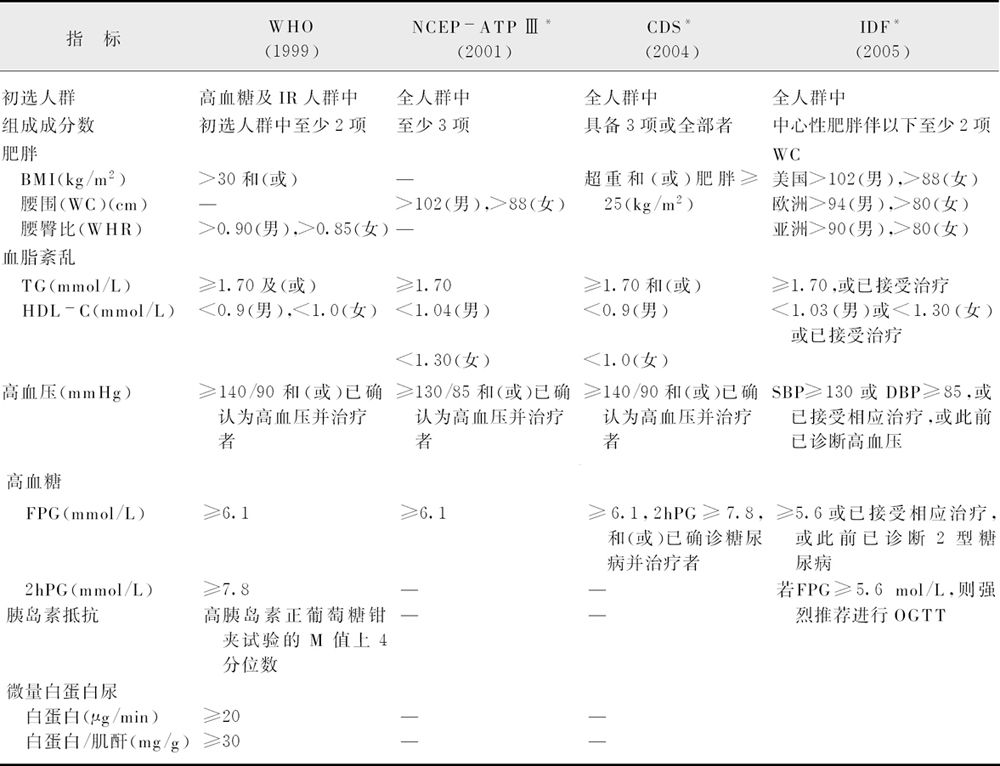
\includegraphics[width=5.94792in,height=1.08333in]{./images/Image00016.jpg}
\end{table}



\paragraph{一、肺念珠菌病}

有关肺念珠菌感染在临床上是多见还是很少见的问题一直存在争议。我国16家医院参加的肺真菌病调查显示该病仅次于肺曲霉病,位列第二。此病为白念珠菌或其他念珠菌所引起的急性、亚急性或慢性肺炎。感染途径主要是吸入,其次为血源性播散。临床上分为念珠菌支气管炎和念珠菌肺炎。支气管炎型表现为阵发性刺激性咳嗽,咳多量白泡沫塑料状稀痰,偶带血丝,随病情进展,痰稠如干糨糊状。憋喘、气短,尤以夜间为甚。乏力、盗汗,多不发热。X线仅示两肺中下野纹理增粗。肺炎型多发于免疫功能低下的患者,表现为畏寒、高热,咳白色泡沫黏痰,有酵臭味,或呈胶冻状,有时咯血,临床酷似急性细菌性肺炎。胸部X线显示双下肺纹理增多,纤维条索影伴散在的大小不等、形状不一的结节状阴影,呈支气管肺炎表现;或融合的均匀大片浸润,自肺门向周边扩展,可形成空洞。双肺或多肺叶病变,病灶时有变化,但肺尖较少受累。偶可并发渗出性胸膜炎。

诊断肺念珠菌病,要求合格的痰液或支气管分泌物标本2次显微镜检酵母假菌丝或菌丝阳性,以及真菌培养连续2次以上有同一菌种生长。另外,血清1,3-β-D-葡聚糖抗原检测连续2次阳性可做诊断参考。组织活检见有念珠菌菌丝侵入及炎症细胞浸润,可以确诊。

\paragraph{二、肺曲霉病}

肺曲霉病主要由烟曲霉引起,临床上主要有五种类型:侵袭性肺曲霉病、气管支气管曲霉病、慢性坏死性肺曲霉病、曲霉肿和变应性支气管肺曲霉病(ABPA)。这些类型的病变临床表现并不一样。

侵袭性肺曲霉病是最常见的类型,症状以干咳、胸痛常见,部分患者有咯血,病变广泛时出现气急和呼吸困难,甚至呼吸衰竭。部分患者可有中枢神经系统感染。中性粒细胞缺乏患者其X线胸片显示以胸膜为基底的多发的楔形阴影或空洞,病变早期胸部CT为晕轮征(halo
sign),后期为新月体征。但慢性阻塞性肺疾病合并侵袭性曲霉病时典型的CT改变很少见,而非特异性肺实变更多见。

气管支气管曲霉病病变主要在大气道,症状为发热、频繁咳嗽、少痰、胸痛、咯血。支气管镜检可确诊,可见气管支气管内假膜、溃疡、结节等病变。

慢性坏死性肺曲霉病亦称半侵袭性肺曲霉病,患者有长期呼吸道症状如咳嗽、咳痰等,也多有发热。X线显示慢性肺部空洞性病变。

曲霉肿(曲菌球)常继发于支气管囊肿、支气管扩张、肺脓肿和肺结核空洞。继发感染时可有发热,症状主要是刺激性咳嗽,常反复咯血,甚至大咯血,痰量一般不多。X线胸片显示在原有的慢性空洞内有一随体位改变而在空腔内移动的团球影。

ABPB为对曲霉过敏者吸入大量孢子后出现发热、喘息、畏寒、乏力、刺激性咳嗽、咳棕黄色脓痰,偶带血。患者多有哮喘病史。哮喘样发作为其突出的临床表现。X线胸片为上叶短暂性实变或不张,一过性肺浸润,磨玻璃阴影伴马赛克征。中央性支气管扩张(肺野内侧2/3的支气管)及壁增厚征象,有黏液嵌塞时表现为指套征或手套征。上述病变可发生于双侧。诊断标准见表\ref{tab2-12}。

\begin{table}[htbp]
\centering
\caption{ABPA诊断标准}
\label{tab2-12}
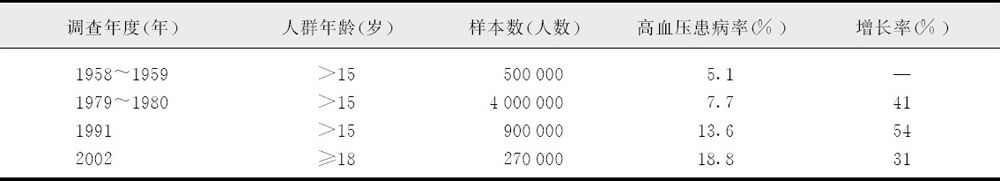
\includegraphics[width=5.97917in,height=1.84375in]{./images/Image00017.jpg}
\end{table}

诊断肺曲霉病除职业史(鸟禽饲养者、酿造工人、农业接触发霉稻谷者等)、机体免疫状态、临床表现及X线检查外,确诊有赖于组织培养及组织病理学检查,或呼吸道标本培养阳性,涂片见菌丝。血清曲霉抗体测定和血、尿、脑脊液及肺泡灌洗液曲霉半乳甘露聚糖测定和PCR测定血中曲霉DNA对本病诊断亦有帮助。变应性支气管肺曲霉病患者的诊断需与支气管哮喘相鉴别。

\paragraph{三、肺毛霉病}

肺毛霉病少见。此病常继发于糖尿病、肝硬化、结核病、恶性肿瘤、白血病及慢性感染的基础上,一般发生于终末期病变。病理改变主要为急性化脓性肺炎、多数性肺脓肿形成与肺坏疽。临床症状无特异性,主要为咳嗽、咳粉红色与黄红色痰、发热与白细胞增多。此霉可向全身播散,侵犯各脏器(心、肾、脑、肺等)。胸部影像学检查(尤其是胸部CT)可以显示单发或多发性浸润影或结节影,有时呈楔形改变,好发部位多为上叶,可双肺同时受累,下叶较少见。诊断有赖于组织病理学。

\paragraph{四、肺隐球菌病}

肺隐球菌病是由具有致病性的新生隐球菌及其变种感染引起的急性或亚急性肺真菌病,近年患病率有增加趋势。隐球菌经呼吸道侵入,在肺内形成感染灶,本病可呈急性、慢性或血源性播散,常引起隐球菌性脑膜炎。免疫抑制宿主(如AIDS)和健康人均可发病。临床分为无症状型、慢性型和急性型。急性型患者可有发热、咳嗽、咳黏液痰,盗汗、乏力和体重减轻。少数病例呈急性肺炎表现,高热、气急、低氧血症,可导致急性呼吸衰竭。以下线索诊断时可参考:①原先健康者肺部X线显示孤立或多发性结节状或块状阴影,特别是病变位于胸膜下时,常有空洞形成;毒性症状不明显;②免疫抑制患者出现肺部浸润,可单侧或双侧,可出现弥漫性间质性改变或粟粒状阴影;③肺部病变伴有脑膜炎表现者。

诊断可用痰涂片采用墨汁染色,可见圆形厚壁孢子,可有出芽现象,孢子内有反光颗粒,可提示诊断。组织活检可作最后诊断。播散型隐球菌病可做血、尿、脑脊液、皮肤损害的脓液等涂片及培养检查,阳性者可诊断。此外,乳胶凝集试验检测隐球菌荚膜多糖体抗原检测也有助诊断,非脑膜炎患者血清的阳性率为20\%~50\%。

\paragraph{五、肺孢子菌肺炎}

长期以来肺孢子菌一直被划归为原虫,但DNA研究证实肺孢子菌更接近于真菌,同源性介于子囊菌和担子菌之间。近年来核酸序列分析显示,人类与动物中分离出来的肺孢子菌差异很大。因此,国际上将从人类中检出的病原体改名为耶氏肺孢子菌(pneumocystis
jiroveci),而寄生于大鼠的则命名为卡氏肺孢子菌。同时建议保留PCP的缩写用法,但其含义改为肺孢子菌肺炎(pneumocystis
pneumonia)。肺孢子菌肺炎是免疫功能低下患者最常见以及最严重的机会感染性疾病之一。近年来发病率急剧增加,与免疫抑制剂、器官移植和艾滋病的流行有关。其感染途径主要为空气传染和体内潜伏状态肺孢子菌的激活。临床上分为流行型(经典型)与散发型(现代型)。流行型主要发生于2~6个月龄的早产儿、营养不良儿;散发型好发于免疫缺陷、肿瘤化疗、长期应用糖皮质激素或免疫抑制剂的儿童和成人。起病缓慢,早期有低热、腹泻、纳差、体重减轻,继而出现干咳、进行性呼吸困难、发绀等,常发生呼吸衰竭。体征常缺如,与症状的严重程度分离。胸部X线检查早期典型改变为双侧肺门周围弥漫性渗出,呈网状和小结节状影,然后迅速进展成双侧肺门的蝶状影,呈肺实变,可见支气管充气征。本病诊断有赖于活检组织特殊染色找到病原体。有文献报道实时定量PCR检测敏感性98\%,特异性96\%,可帮助分辨患者是否为PCP感染期。

艾滋病患者中PCP是最重要的机会感染之一,约85\%左右的晚期艾滋病患者合并PCP,25\%的艾滋病患者死于本病。近年国内报告的一组200例艾滋病患者中,已确诊PCP的有12例,其中4例合并结核病,1例合并肺炎链球菌肺炎。患者均有发热、咳嗽,干咳无痰;体温37.5~39.0℃,其中10例有呼吸急促、呼吸困难、发绀。肺部听诊2例有肺底部少许可变性湿啰音,2例少许干啰音。治疗前患者痰PCR检测均阳性,血PCR检测9例阳性;六胺银染色、吉姆萨染色找卡氏肺孢子菌分别有5例和6例阳性。

\subsubsection{3.1.8 寄生虫感染}

\paragraph{一、阿米巴肺脓肿}

阿米巴肺脓肿目前已比较少见。病变通常位于右下肺,因此病多由阿米巴肝脓肿穿破横膈至肺所引起,胸膜也同时累及。有时左叶肝脓肿向左膈穿破而引起左侧胸膜、肺阿米巴病。在少数病例中,阿米巴原虫由肠道病灶经血行传播至肺部,有些病例可无肝或肠阿米巴病病史,形成所谓“原发性肺阿米巴病”,易使人误会病变原发在肺。肺阿米巴病患者就诊时往往以发热、咳嗽、咳痰、右下胸痛与右肩放射痛为主诉,发热多为高热,弛张热型,伴或不伴寒战,可有气促、盗汗、纳差等症状。脓肿破入支气管时咳出大量酱红色或巧克力色黏稠脓性痰,对提示本病的诊断有重要意义。体检可发现肝脓肿体征。腹部B超和CT有助于诊断。

阿米巴肺脓肿的主要诊断依据是:①肠道或肝阿米巴病的病史;②大量典型的酱红色或巧克力色黏稠脓性痰,可检出溶组织阿米巴滋养体,但阳性率低于20\%;③右下肺叶病变,以及在X线透视下右膈局限性隆起与运动减弱等;④对甲硝唑(灭滴灵)治疗具有迅速而显著的疗效。疑似病例应考虑作抗阿米巴诊断性治疗。

\paragraph{二、急性血吸虫病的肺部病变}

急性血吸虫病较常并发肺部病变。肺部病变的出现距离感染期40余天至2个月左右,约2~3个月之后吸收并遗留少许痕迹。患者的临床表现有发热及其他毒血症症状等,伴有肝大压痛与外周血嗜酸性粒细胞增多。呼吸道症状大都轻微,咳嗽较常见,偶尔有咯血;胸部体征甚少,可有干、湿啰音。X线所见主要为弥漫性浸润,按其病灶显示的形态,可分为:①小斑片状阴影;②片状阴影;③大片状阴影;④粟粒状阴影等四类。

急性血吸虫病肺部病变的主要诊断根据是:①患者有急性血吸虫病的证据;②上述的肺部症状与X线征;③除外其他原因的肺部病变;④吡喹酮治疗疗效良好。

\paragraph{三、人比翼线虫病}

人比翼线虫病系罕见的疾病。自1913年发现以来,据报道全世界病例约100例。国内曾报道3例,一起进食未煮熟的鳖而致感染。主要症状为慢性阵发性咳嗽与咳黄痰,病程1个月后有血痰,体重减轻,亦可有胸痛。抗生素治疗无效是本病的特点。痰沉渣涂片检查可找到虫卵,孵化后虫壳内可见到幼虫。胸部X线表现无特殊性,大多数无异常发现,有的可表现为支气管炎或肺炎。纤维支气管镜检查所见主要表现为支气管黏膜充血,可有肉芽肿形成。特征表现是气管支气管内可见鲜红色血丝样的Y形线虫,钳出体外可见虫体蠕动。如怀疑此病可嘱患者仔细观察咳出的痰,有时可见虫体而诊断。

\protect\hypertarget{text00026.html}{}{}

\subsection{3.2 变态反应性疾病}

\subsubsection{一、单纯性肺嗜酸性粒细胞浸润症(吕弗勒综合征)}

单纯性肺嗜酸性粒细胞浸润症又称吕弗勒综合征(Löffler's
syndrome),主要特点是短暂而易消散的肺部浸润阴影,伴以短暂的外周血嗜酸性粒细胞增多。多数病例有短期的发热。参考第7.2.3节。

诊断本病的主要依据是:①病程短暂与良性经过;②发热、咳嗽、咳痰,肺部听诊可有干性或湿性啰音等症状与体征;③外周血嗜酸性粒细胞增多;④X线检查肺部有短暂性浸润阴影,呈游走性,消散后不留痕迹。

\subsubsection{二、风湿性肺炎}

风湿性肺炎少见,一般发生于风湿热的基础上。临床表现一般可区分为轻、重两型。轻型病例仅轻微咳嗽,偶有血丝痰,肺部可发现湿啰音,病变局限,可并发胸膜炎,预后较佳,因症状轻微,临床上易被忽视。重型病例病变广泛,往往突然出现脉快、心悸、气促、发绀、胸痛、咳血丝痰等症状,体温波动较大,病情较重,但肺部体征却轻微甚或缺如。X线表现多种多样,出现迅速,消散也快,有时呈游走性反复出现,连续X线检查,对临床诊断常起决定性作用。

风湿性肺炎的诊断主要根据:①有符合风湿热的临床表现;②上述的胸部症状与X线征;③除外其他原因的肺部病变,如过敏性肺炎、肺炎支原体肺炎等。抗链球菌溶血素“O”测定及C反应蛋白反应,对此病的诊断往往有帮助。

\protect\hypertarget{text00027.html}{}{}

\subsection{3.3 风湿性疾病}

许多风湿性疾病可有发热和肺部浸润。系统性红斑狼疮可有间质性或小叶性肺炎等肺部表现,常与胸膜炎并发。狼疮性肺炎表现为发热、干咳、气促,X线胸片可见片状浸润阴影,多见于双下肺。因多有白细胞减少,且抗生素治疗无效,可误诊为病毒性肺炎,但激素治疗后肺炎迅速消退。类风湿关节炎、系统性硬化病、多发性肌炎-皮肌炎等可有发热和肺部浸润病变,结节性多动脉炎的肺部病变多伴有咯血。临床上应注意鉴别,目前由于免疫学检查的普及,诊断一般不难。

\protect\hypertarget{text00028.html}{}{}

\subsection{3.4 化学性及物理性损害}

\subsubsection{一、化学性肺炎}

在化学工业生产过程中或其他原因而致吸入高度刺激性的化学性气体(如氮氧化物、硫化氢、氯、二氧化硫、汽油等),可引起急性肺部病变,表现为肺炎与急性肺水肿。

\paragraph{(一)汽油吸入性肺炎}

患者以汽车司机及其助手为多见,一般在吸入后立即发生剧烈咳嗽,并常有咯血,2~8小时后体温开始上升,大多数持续于38~39.5℃之间,最高达40℃以上。其他常见症状为胸痛、头痛、头晕、昏厥、恶心、呕吐、呼吸困难等。体检出现肺部浊音、肺泡呼吸音减弱、湿啰音等。X线检查在发病后3~6小时内,一般即可发现肺部大片密度不均匀,边缘模糊的实变阴影,后者与肺门相连,其周围有散在性、密度不甚高的斑点状阴影。此病如能及时恰当处理,一般预后良好。

\paragraph{(二)胃酸吸入性肺炎}

系胃酸反流吸入引起的化学性肺炎,亦称孟德尔森综合征(Mendelson
syndrome)。以年长者居多。临床上以胃酸反流后出现咳嗽、发热、呼吸困难为主要表现,继而出现急性呼吸窘迫综合征(ARDS)。本病国外报道较多,临床对发热、很快出现呼吸窘迫、发绀的患者,尤其是老年患者应注意鉴别。

\subsubsection{二、药物性肺病}

有些药物如呋喃妥因、青霉素、碘、复方乙酰水杨酸、异戊巴比妥等可引起变态反应性肺部病变,发病急,表现为发热、全身性皮疹、双肺湿啰音、X线胸片呈斑片状阴影等。诊断时需仔细寻找用药史。

\subsubsection{三、急性放射性肺炎}

急性放射性肺炎是由于放射线治疗胸部疾病(如支气管肺癌)所引起的一种合并症。此病发病较急,预后不良,目前尚无有效疗法。急性放射性肺炎的诊断主要根据下列各点:①病史:胸部曾接受大面积高剂量的放射治疗,发病前有感冒史;②症状:干咳、气促、微热,进行性病情加重;③体征:有发绀、呼吸困难,照射区内叩诊浊音,并可听到湿性与干性啰音;④化验检查:白细胞总数不增多;⑤肺部X线检查:照射野内有密度增高的片状或网状阴影,尤以肺门区为显著。

\protect\hypertarget{text00029.html}{}{}

\subsection{3.5 特发性间质性肺炎}

\subsubsection{一、急性间质性肺炎}

急性间质性肺炎(AIP)又称Hamman-Rich综合征,是一种病因未明、起病急骤、病情危重,以肺部弥漫性浸润并迅速发展为呼吸衰竭为特征的肺部疾病。患者起病突然、进展迅速,在较短时间内出现呼吸衰竭,平均存活时间很短,大部分在1~2个月死亡。绝大部分患者在起病初期有类似上呼吸道病毒感染的症状,半数以上的患者突然发热、干咳,伴进行性加重的呼吸困难。双肺底可闻及散在的细捻发音。实验室检查不具有特异性。X线胸片显示双肺广泛弥漫性浸润阴影。近年国内文献已有报道。本病临床表现为病情急剧进展的急性呼吸系统疾病,患者有发热、咳嗽、进行性呼吸困难乃至快速导致呼吸衰竭。X线胸片显示双肺广泛弥漫性浸润阴影。病因与发病机制尚未明了。诊断须排除各种已知原因的急性肺疾病方能确定,尤须与ARDS相鉴别,主要根据临床和病理的认真分析以及糖皮质激素的治疗效果。

\subsubsection{二、隐源性机化性肺炎}

隐源性机化性肺炎(COP),指不明原因的机化性肺炎(OP),是一种以细支气管、肺泡管、肺泡腔内肉芽组织栓形成为特征的肺部非特异性炎症过程,包括继发性机化性肺炎和隐源性机化性肺炎(COP)。后者指没有明确病因的“特发性”机化性肺炎。以往曾称为闭塞性细支气管炎伴机化性肺炎(BOOP)。该病主要表现为干咳、呼吸困难,呼吸困难多为活动后气短,程度多数较轻,部分患者可出现发热、纳差、体重下降。胸片可表现为双侧斑片状浸润影,主要分布于胸膜下及肺野外带,在病程中可有游走性。胸部CT表现分为:①多发性肺泡实变影(典型COP):多见于双肺胸膜下或沿支气管血管束分布,病变大小从几厘米到整个肺叶不等,可有支气管充气征及游走性表现。②浸润性阴影(浸润性COP):表现为双肺底网织状阴影伴磨玻璃影,浸润型由定义不清的弓形病变或小叶旁的多角形病变组成,通常伴随着其他阴影尤其是实变影。③局灶性实变影(局灶COP):局灶肺泡浸润影常位于上肺,边缘清楚,常呈叶、段分布,偶有空洞。肺部影像学具有多发性、多态性、易变性和病变多在肺外周的特点,加上抗生素治疗无效,临床诊断并不困难。糖皮质激素治疗效果一般较好。

\protect\hypertarget{text00030.html}{}{}

\section{4 周期性发热}

患者的体温突然或徐缓上升到高峰,保持数小时乃至若干天,然后迅速或徐缓下降至正常,经若干天无热期后又再发热,历数小时至若干天后又下降至正常。如此发热期与无热期互相交替,反复多次,即周期性发热。周期性发热原因可分为感染性与非感染性两类(表\ref{tab2-13})。

\begin{table}[htbp]
\centering
\caption{周期性发热的疾病分类}
\label{tab2-13}
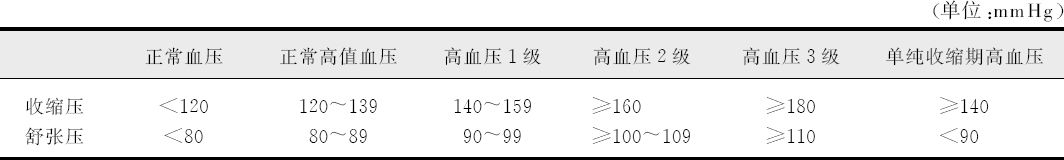
\includegraphics[width=5.92708in,height=2.9375in]{./images/Image00018.jpg}
\end{table}

\subsection{4.1 感染性周期性发热疾病}

\subsubsection{一、波状热(布鲁菌病)}

波状热的主要传染源是受感染的羊、牛与猪。文献报告约15\%~22\%病例具有典型的波状热型、每次发热期自6天至数周不等,一般有几个热波,可自行退热而进入缓解期,经数天至数周,热度又见回升。此种反复发生的周期性发热可迁延累月经年之久(参见第5.1节)。

\subsubsection{二、局灶性细菌性感染}

肾盂肾炎、支气管扩张合并感染、血栓性静脉炎、胆囊炎等部位处受到细菌性感染,都可引起反复的发热或寒战发作,但间歇期并无规则。

一侧慢性腰痛伴有原因未明的间歇性发热,除慢性复发性肾盂肾炎之外,肾结核也须考虑。国内报告不典型肾结核,可仅以间歇性发热为临床的唯一表现。

对于反复发生细菌性感染的患者,尤其是同类病原体引起的反复感染(如肺炎双球菌性肺炎),应考虑低(或无)丙种球蛋白血症或无能丙种球蛋白血症的可能。低(或无)丙种球蛋白血症可为先天性或获得性。诊断方法主要是测定血清中免疫球蛋白定量,缺乏IgG或7S丙种球蛋白时,抗细菌、抗病毒的抗体也常缺乏,致反复发生感染。无能丙种球蛋白血症与低丙种球蛋白血症不同,患者的血清蛋白电泳有高于正常或正常量的丙种球蛋白,只是表现丙种球蛋白的功能有缺陷,免疫功能低下,对各种感染有极大的易感性,人工自动免疫试验无抗体形成(如接种伤寒菌苗后,肥达反应阴性)。本症可为特发性或继发性,常继发于骨髓瘤、淋巴瘤、白血病等。

\subsubsection{三、败血症、亚急性感染性心内膜炎}

在败血症与亚急性细菌性心内膜炎病例中,有时可出现间歇性发热,类似疟疾发作,如不注意详细检查,可致误诊(参见第1.1节)。

\subsubsection{四、回归热}

回归热是由回归热螺旋体引起的急性虫媒传染病,引起人类发病者有虱传和蜱传回归热螺旋体,前者国内已罕见报道,后者散发于世界各地,我国以南疆及山西等地为主要发病地。本病特点为急起急退的高热,短期热退呈无热间歇,数日后又反复发作,发热期与间歇期交替反复出现,并有全身肌肉酸痛、肝脾大。间歇期除感虚弱外,其他症状均减退或消失,血白细胞多增高,也可正常,中性粒细胞增多。发作次数频繁者贫血严重,可有丙氨酸转氨酶升高,凝血酶原时间延长等,发热期采血涂片检出螺旋体可确诊。

回归热可分为流行性回归热与地方性回归热二型。前者以体虱为传染媒介,症状较重;后者由壁虱传播,症状较轻。

在流行性回归热多发的冬春季节及地区,如患者有寒战、高热、头痛、肌痛、鼻出血,并发现带虱或曾与此病患者有密切接触史者,须考虑此病的可能性,应作厚滴血片或血涂片镜检回归热螺旋体。

据国内报告;地方性回归热发病季节以4~8月为高,有严格的地区性,诊断地方性回归热须注意以下几点;①发病急骤.发热呈不规则的间歇型,初次发作持续时间为2~6天。以后发作仅持续数小时至一天。无热期长短不一,自1~14天,因而呈现不规则的周期性发热曲线。②症状较流行性回归热为轻。③患者无带虱现象,反之往往有被壁虱刺咬史。④血液及骨髓涂片中螺旋体数量虽稀少难找,但在无热期也可找到;动物接种易于成功。⑤青霉素治疗无效,胂剂一次疗法大都复发。

有报道:女,17岁,新疆人,周期性发热3个月,每周发热1~3次,午后发热,体温达40℃,中度贫血,血涂片检出回归热螺旋体,青霉素治疗14天,未再发热。

回归热须与钩端螺旋体病、流感、斑疹伤寒、疟疾、波状热等相区别。可依靠流行病学史、临床动态观察、病原学与血清学检查,一般困难不大。

\subsubsection{五、鼠咬热}

鼠咬热罕见。引起鼠咬热的病原体已证实有两种:一为小螺旋体,一为念珠状链杆菌。国内报告的病例大都由前者引起。由后者引起的仅属个别病例。

诊断鼠咬热首先须注意鼠咬史。由小螺旋体引起的鼠咬热有以下临床特征:潜伏期5~21天。患者通常以寒战、高热急骤发病,全身症状较重。最有诊断价值的特征是在鼠咬部位发生热、肿、痛,呈紫黑色,可形成水疱、组织坏死或硬性下疳样溃疡,上覆以黑色痂皮,并有局部淋巴结炎。发热持续数天而骤退,但经数天后又再发,呈回归热型、发热期间鼠咬伤部位炎症加剧,患者可发生皮疹,抽血作暗视野荧光检查,可发现活动迅速的小螺旋体,在皮肤损害处采取分泌物或肿胀的局部淋巴结穿刺检查,更易获得阳性结果。胂剂或青霉素治疗有效。

由念珠状链杆菌引起的鼠咬热,症状基本与上述相似,但潜伏期较短,仅1~5天,咬伤处炎症反应不显著,胂剂疗法不理想,但青霉素治疗有良效。可将患者血液作培养或接种于小白鼠腹腔内而确定诊断。

鼠咬热须与疟疾、回归热、斑疹伤寒及败血症等相鉴别,主要根据鼠咬史与病原学检查。

\subsubsection{六、间日疟}

凡在夏、秋季节,患者有周期性发冷、发热、盛汗,呈隔日发作兼有脾大与贫血,须考虑间日疟的可能性。如患者在疟区居留或最近曾到过疟区,间日疟的临床诊断大致可以成立。血涂片发现间日疟原虫是确诊的可靠依据。

在各种疟疾中,间日疟较为多见。分布也较广。潜伏期通常为10~14天,输血疟疾则较短(7~10天)。

患者以突然寒战急骤发病,颜面苍白,虽盖厚被仍未能止冷。发冷持续约1/2~2小时,继而体温迅速上升,高热往往达40~41℃。此时患者颜面转为潮红、头痛、口渴,有时谵妄;皮肤干热,脉快。发病5~7小时后开始大量出汗,持续约2~3小时衣摆尽湿,体温恢复正常或降至常温以下。整个发作过程持续6~10小时,单纯感染者每隔48小时周期发作一次。发作多在中午至下午,经数次发作后,脾脏可触及,并出现继发性贫血。有的病例出现唇疱疹,对诊断有一定意义,因唇疱疹少见于其他类型疟疾。

典型间日疟的临床诊断较易,但二重感染者、混合感染者(常见是间日疟合并恶性疟)以及曾接受不规则抗疟治疗者症状常不典型,易误诊为其他急性发热疾病。此时作厚滴血片或血涂片镜检疟原虫是确定诊断的最简捷方法。如厚滴血片阴性,必要时可作骨髓穿刺涂片检查。口服氯喹作诊断性治疗可用于高度疑似的病例。

\subsubsection{七、三日疟}

三日疟比较少见,大多为散发性。病初发热不高,呈不规则型、弛张型热,3~5天后较为典型发作,症状与间日疟相似。有发冷、发热及出汗阶段,但每隔72小时发作一次,且多在午后发作。单纯感染者发作周期经常不变。发作数次后出现脾大与贫血。

三日疟的临床诊断可根据典型的周期性发作、脾大与继发性贫血。二重感染者可每发作二天间歇一天,三重感染者可每天发作,因而必须注意与其他发热性疾病相鉴别。血涂片镜检发现三日疟原虫是诊断的最可靠依据。

\subsubsection{八、蛋形疟}

蛋形疟是最少见的疟疾,流行季节为4~7月和10~12月。蛋形疟的发作周期与间日疟同,也为48小时,但其发作常在黄昏或晚间。临床症状轻重不一,轻症者可无明显症状,重症者发热可达41℃或以上,并可持续十余小时之久,甚至发生谵语。此病在治愈后不易复发。确诊须依靠从血液中检出蛋形疟原虫。

\subsubsection{九、黑热病}

有些黑热病患者的早期症状与波状热相似,体温曲线呈波状起伏,并有大量出汗,脾大与白细胞减少。这种情况甚至使人不会想到黑热病。偶尔早期患者的血清可凝集布鲁菌,但滴度不超过1∶160。另一方面,有时早期黑热病的症状可酷似间日疟,但血片镜检疟原虫始终阴性,抗疟治疗无效。

黑热病的诊断须根据流行病学史、临床表现与骨髓穿刺检查。

\subsubsection{十、丝虫病}

丝虫病患者发作丝虫热时,通常在剧烈运动或疲劳之后,突以畏寒或寒战而起病。继而体温急骤上升,可达40℃,伴淋巴管(结)炎,持续1~3天而消退,但也可持续达一周之久。往往每隔2~4周或数月发作一次。

\subsubsection{十一、战壕热(五日热)}

战壕热可以每隔五天出现寒热发作为特征,并有皮疹,腰、腿肌痛与胫骨痛,病程长短不一。此病是一种立克次体感染,传染媒介为体虱,国内未发现。

\subsubsection{十二、其 他}

偶见有钩虫病致周期性发热3个月,间歇3~4天发热1次,持续3~4小时自退,患者有嗜酸细胞增多,贫血,大便隐血弱阳性,粪找虫卵阴性。胃镜发现十二指肠降部数条钩虫。

\protect\hypertarget{text00031.html}{}{}

\subsection{4.2 非感染性周期性发热疾病}

\subsubsection{一、结节性脂膜炎}

结节性脂膜炎(Weber-Christian病)是一种原发于脂肪小叶的非化脓性炎症,是较少见的一种变态反应性疾病。好发于青壮年女性。根据受累部位,可分为皮肤型和系统型。

临床表现以反复全身不适、关节痛、发热、皮下结节为特征,受累的皮肤反复发生红斑,时有压痛,并有水肿性皮下结节,损害呈多发性、对称性、成群分布、最常受累的部位是双下肢,常伴全身不适,发热与关节疼痛,亦可出现恶心、呕吐、腹痛、体重下降、肝脾大及其他内脏损害,其病程有很大差异,主要取决于受累器官的情况,内脏受累广泛者,可出现多脏器功能衰竭、大出血或并发感染。

结节性脂膜炎发热的特点:半数以上皮肤型发热可为低热、中度热或高热,热型多为间歇热或不规则热,少数为弛张热,通常在皮下结节出现数日后开始发热,持续时间不定,多在1~2周后逐渐下降;系统型的发热一般较为特殊,常与皮疹出现相平行,多为弛张热,皮疹出现后热度逐渐上升,可高达40℃,持续1~2周后逐渐下降。

实验室检查多为非特异性改变,白细胞总数可正常、增多或减少,血沉快。皮肤结节活检的组织病理学改变是诊断的主要依据。

此病可被误诊为败血症、伤寒、肺结核、颈淋巴结结核、风湿热、结节性红斑、恶性组织细胞病等。凡有发热及皮下结节的病例疑似此病时,应及时作结节活检明确诊断。

\subsubsection{二、风湿热}

风湿热有复发的倾向。

\subsubsection{三、周期性发热综合征}

周期性发热综合征是非常罕见的疾病,作此诊断时必须慎重考虑,患者自幼年即可起病,偶见于成年人,每隔数天、数周或数月发作一次。间歇期患者俨如常人,因间歇期近于规则,有时可推测其发作日期。

周期性发热综合征(PFS),具有下列共同特征:①复发性和周期性发热;②发热持续时间大多相同,少则2~8日,多则2~4周,比一般的原因不明发热时间短;③多系统炎症(滑膜、浆膜及(或)眼、皮肤等炎症表现);④自限性;⑤实验检查中急性期反应物显著升高,但始终查不到感染性病原,迄今也未查到任何自身免疫疾病的特征;⑥在无症状间歇期患者可完全正常。吲哚美辛或糖皮质激素治疗能迅速解热。

目前按照间歇期的不同形式作为分型基础:①无热间歇期固定的PFS包括周期性中性粒细胞减少症,PFAPA综合征;②无热间歇期不固定而有所变异的PFS(高IgD综合征等);③缺乏无热间歇期的PFS。

国内曾报告个别周期热病例,患者发热期间伴有关节酸痛、皮疹。白细胞增多、血沉加快等表现,反复发作周期热,各项检查均无特殊发现,未接受任何治疗,发热周期自行停止,随访22年未能弄清病因。

\subsubsection{四、痛 风}

痛风每次发作时可伴有发热。

\subsubsection{五、恶性组织细胞病}

此病偶尔可以周期性发冷发热、多汗为主要表现。

\subsubsection{六、恶性淋巴瘤}

恶性淋巴瘤易引起发热,文献报告可达31\%~50\%,且可以发热为初发症状,而此时尚无其他明显的临床表现。热型种类不一,而回归型热(周期热)约见于1/6的霍奇金淋巴瘤,具有一定的特征性。每一发热周期持续2~4周不等。

周期性发热而无浅表淋巴结肿大的恶性淋巴瘤,病变通常位于腹腔、腹膜后、纵隔等处的淋巴结或结外病变,诊断常有困难,须与其他原因的周期性发热疾病相区别。患者常有多汗、疲乏、消瘦或相应结外病变的表现,根据深部淋巴结或结外病变的部位行病灶活检方能确诊。

有报道女,51岁,周期热4年,每次发热伴有咳嗽、咳痰,抗生素治疗效果欠佳,胸部CT显示右肺中叶及左肺下叶实变,误为肺炎,后支气管镜检查肺活检示肺黏膜相关淋巴组织型边缘区B细胞淋巴瘤。提示少数非霍奇金淋巴瘤患者也可表现为周期性发热。

\subsubsection{七、嗜铬细胞瘤}

嗜铬细胞瘤的主要表现是高血压。高血压多为阵发性,发作时可伴有体温升高、头痛、出汗等表现。国内曾有个别病例报告,以突发性间歇性发热住院多次,并疑为疟疾,最后经详细检查方证实为嗜铬细胞瘤。

\protect\hypertarget{text00032.html}{}{}

\section{5 长期发热}

长期不明原因发热(FUO)是指发热持续3周以上,体温≥38.5℃,经完整的病史询问、体格检查及常规实验室检查后仍不能明确诊断者。这类患者的临床表现不典型或病情不呈典型临床经过;或临床医生对某些少见疾病或病变认识不足;某些疾病的病灶隐蔽,不易为常规检查手段所发现等因素所致难以明确发热的病因。

国外对特殊人群的FUO有着特别的定义:

\subsection{1.人类免疫缺陷病毒(HIV)阳性者}

体温≥38.3℃超过4周,其中住院患者热程超过3日仍不能明确病因即可诊断。

\subsection{2.粒细胞缺乏者}

外周粒细胞计数<0.5×10\textsuperscript{9}
/L,体温≥38.3℃超过3日,培养阴性2日以上。

\subsection{3.老年患者}

除病者为老年人外,其他标准同经典的FUO。

\subsection{4.住院患者}

因非感染性疾病而入院的患者,发热超过3天病因不能明确者。

长期发热的热型可以多种多样;但以弛张热及不规则热等热型为多见。热程长短对FUO诊断具较大的参考价值。一般来讲,热程短,有乏力、寒战等中毒症状者,有利于感染性疾病的诊断;如热程中等,但呈渐进性消耗、衰竭者,以肿瘤多见;热程长,无毒血症症状,但发作与缓解交替出现,则有利于结缔组织病的诊断。

可引起FUO的病因超过200种,长期发热的原因是复杂的,除中枢性原因外,可概括为以下四大类(表\ref{tab2-14}):

\begin{longtable}{c}
 \caption{长期发热疾病}
 \label{tab2-14}
 \endfirsthead
 \caption[]{长期发热疾病}
 \endhead
 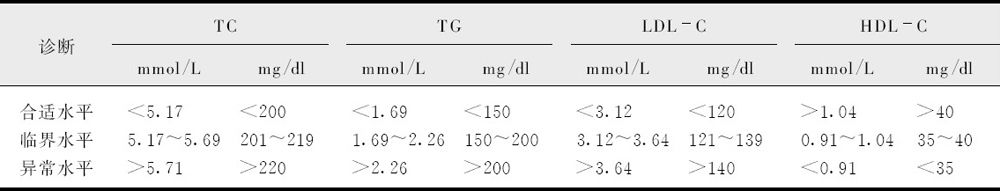
\includegraphics[width=\textwidth,height=\textheight,keepaspectratio]{./images/Image00019.jpg}\\
 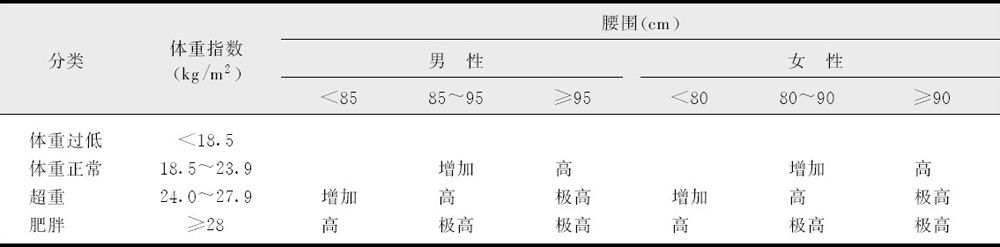
\includegraphics[width=\textwidth,height=\textheight,keepaspectratio]{./images/Image00020.jpg}
 \end{longtable}

\subsection{一、感 染}

感染是长期发热最常见的原因。在各种感染中,结核病是主要原因之一,特别是某些肺外结核,如深部淋巴结结核、肝、脾结核尤难于诊断;早期的急性粟粒型结核和脊椎结核也难于诊断。

其他感染还有伤寒与副伤寒、亚急性感染性心内膜炎、布鲁菌病、败血症、阿米巴肝病、CMV病毒、HIV、真菌等。

\subsection{二、血液病}

不明原因发热中以淋巴瘤所占比例最高,常成为诊断难题。

发热、出血、进行性贫血,肝、脾、淋巴结肿大,可提示血液病诊断的线索。

\subsection{三、风湿性疾病}

风湿性疾病的临床表现多种多样,其中,发热可以为首发症状,亦可在病程中出现。有报道各种风湿性疾病出现发热的几率排列为:Still病100\%,SLE
70\%~80\%,干燥综合征20\%,肌炎及(或)皮肌炎10\%,系统性硬皮症约5\%。其中Still病约占结缔组织病发热的50\%。临床上两个以上互不相关的器官损害表现可提供结缔组织病的诊断线索,其中以多发性关节炎与皮疹是最常见的共同表现,且往往早期出现,还可出现心、血管、肝、肾、肺、肌肉等器官和组织的损害。其实验室检查的特点是自身抗体及高免疫蛋白血症。

\subsection{四、恶性肿瘤}

恶性肿瘤生长迅速,当肿瘤组织崩溃或合并感染时则可引起长期发热。如肝癌、结肠癌,早期易漏诊。血清乳酸脱氢酶活性、癌胚抗原(CEA)、甲胎蛋白(AFP)等测定有助于诊断。

李龙芸回顾了1953-1997年《中华内科杂志》刊出的124例病例的临床病理(例)讨论见表\ref{tab2-15}及表\ref{tab2-16},确诊方法:尸检85例,开胸探查5例,开腹探查11例,组织活检15例及实验室检查8例。疑难发热病病因以感染性、血液系统及肿瘤疾病为主,分别为36.4\%、30.2\%及20.9\%。感染性疾病中以细菌性及结核性感染为主,其次为病毒性、寄生虫性及霉菌性感染。血液性疾病中以淋巴瘤、恶性组织细胞病为主。结核性疾病及寄生虫感染无减少趋向,病毒及霉菌性感染报道增多,尤其艾滋病、卡氏肺孢子菌肺炎及巨细胞病毒。对疑难发热病例应警惕结核、细菌性感染及寄生虫、淋巴瘤、恶性组织细胞病、恶性肿瘤等。这组患者结核病以中青年为主,热程1~18个月,平均(6.1±5.7)个月。淋巴瘤大多数热程超过1年。恶性组织细胞病10天~3年,平均(6.2±5.7)个月。成人Still病热程1个月~1年,平均5.3个月。

1998-2013年《中华内科杂志》刊出长期不明发热的临床病例讨论29例的病因见表\ref{tab2-17},29例中淋巴瘤占45\%。

\begin{table}[htbp]
\centering
\caption{1953-1997年《中华内科杂志》刊出的47例疑难临床病理讨论的感染性疾病发热的病因}
\label{tab2-15}
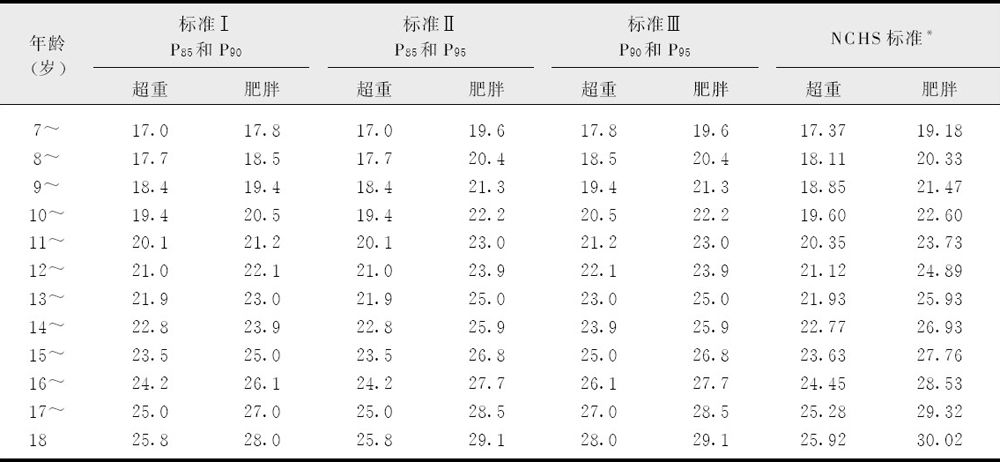
\includegraphics[width=5.94792in,height=3.83333in]{./images/Image00021.jpg}
\end{table}

\begin{table}[htbp]
\centering
\caption{1953-1997年《中华内科杂志》刊出发热疑难临床病理讨论的肿瘤、血液、结缔组织病性疾病}
\label{tab2-16}
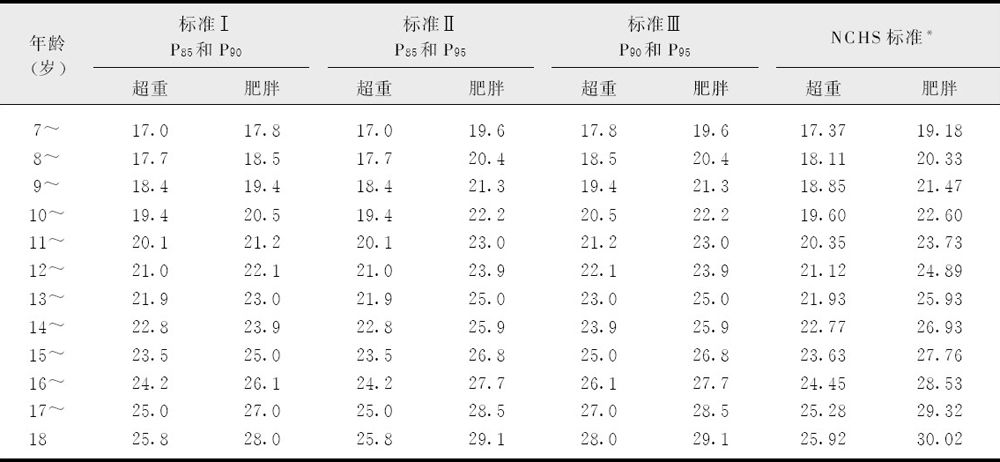
\includegraphics[width=5.95833in,height=4.41667in]{./images/Image00022.jpg}
\end{table}

\begin{table}[htbp]
\centering
\caption{1998-2013年《中华内科杂志》刊出长期不明发热的临床病例讨论29例的病因}
\label{tab2-17}
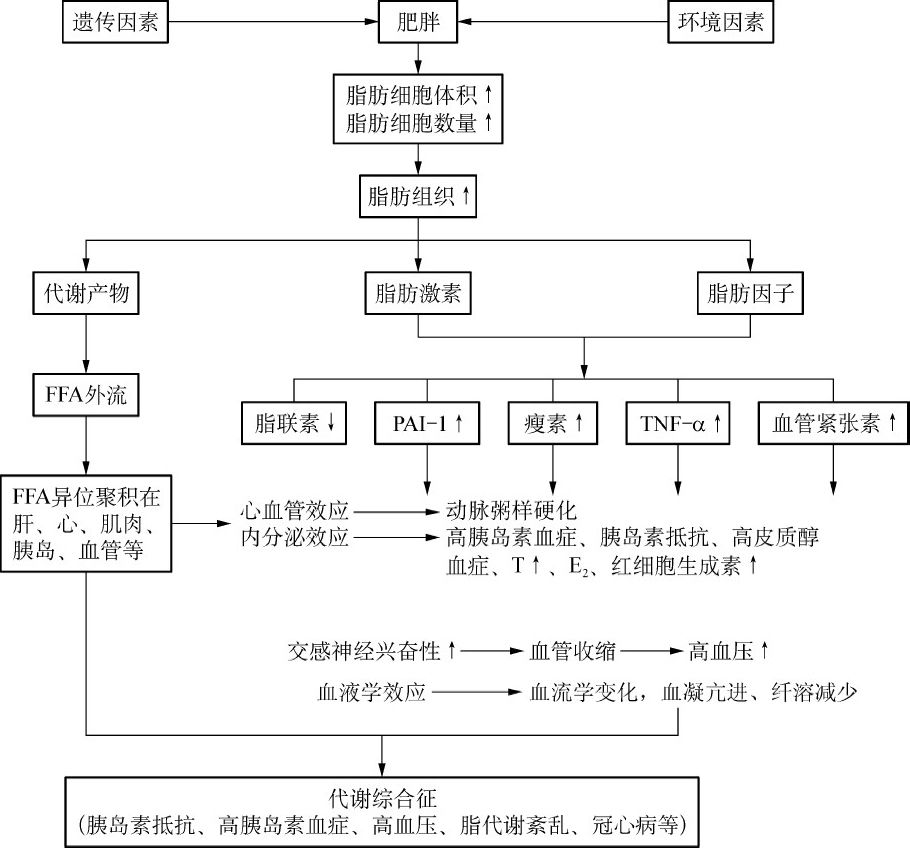
\includegraphics[width=5.95833in,height=2.92708in]{./images/Image00023.jpg}
\end{table}

另有报道一组未明原因长期发热449例(表\ref{tab2-18})。病因包括:感染性疾病(56.8\%),其中结核病占43.6\%;且以肺外结核居多,肺外结核临床表现复杂多样,但大多数患者除长期发热外,常伴乏力、纳差、盗汗、消瘦等结核中毒症状,随着病情进展,有些可出现结核感染部位的症状,也可有血沉增快、γ-球蛋白比值升高、结核菌纯蛋白衍生物(PPD)阳性。一般抗生素治疗无效,需特异性抗结核治疗才有效。PPD强阳性有助于结核病的诊断,但其阴性也不能除外结核诊断。本组有1例腰椎结核患者在院外误诊达15个月之久,故需提高对肺外结核的认识。

此组疾病中结缔组织病19.6\%,其中成人Still病34.6\%,是结缔组织病中引起长期不明原因发热的主要病因。

肿瘤性疾病16.5\%,其中淋巴瘤39.1\%;诊断最困难,因此如怀疑本病建议多次行淋巴结活检,局限于上消化道的淋巴瘤可做胃镜及活检,腹腔内淋巴瘤必要时手术探查,尽早明确诊断,及时治疗。

其他疾病7.1\%,其中坏死性淋巴结炎占33.3\%,药物热占26\%;出院时仍未确诊13.8\%。

\protect\hypertarget{text00033.html}{}{}

\subsection{5.1 感染性疾病}

\subsubsection{一、结核病}

结核病是感染性疾病中引起不明原因长期发热的主要原因。马小军等在2004年的研究显示,449例FUO患者中结核病占21.4\%。侍效春等报道不明原因发热为表现的100例结核病中,可以中高度发热,热型以不规则热为多见,弛张热、稽留热次之,39\%患者有寒战,热程3~77周,中位热程为12周。结核累及部位:单纯肺结核39例,单纯肺外结核28例包括腹腔结核(肠结核、结核性腹膜炎、肝结核、腹腔淋巴结结核)11例、淋巴结(颈部、腹股沟、纵隔)结核4例、结核性心包炎2例、结核性脑膜炎2例及无明确部位9例,肺结核合并肺外结核33例,50\%患者PPD皮试阳性,实验室检查多为ESR增快和C反应蛋白升高以及不同程度的消耗表现即贫血和低白蛋白血症,诊断方法:抗酸杆菌阳性的34例,组织病理符合结核病的8例,临床诊断并经抗结核治疗有效的49例,诊断性抗结核治疗有效的9例。接受抗结核治疗后显效的时间平均为5.3周。从发病至确诊的时间为3~77周,中位确诊时间14周。诊断性抗结核治疗依旧是目前诊断肺外结核的主要方法。对结核病高度可疑病例的诊断性抗结核治疗观察时间放宽到8周,较广为采用的期限4~6周为宜。

\begin{table}[htbp]
\centering
\caption{449例不明原因长期发热的病因分类}
\label{tab2-18}
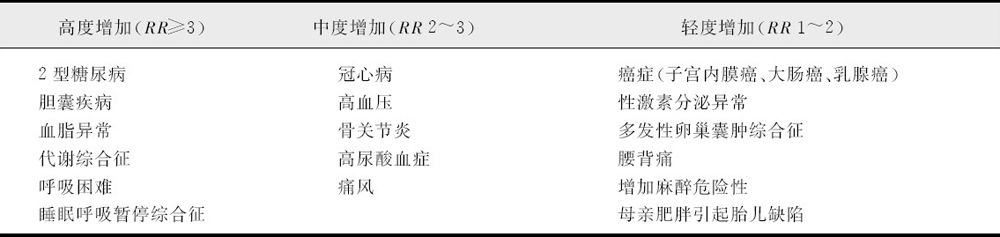
\includegraphics[width=5.97917in,height=8.40625in]{./images/Image00024.jpg}
\end{table}

\paragraph{(一)急性粟粒型肺结核}

过分相信X线胸部透视的阴性结果,可能漏诊急性粟粒型肺结核。易致漏诊或误诊为伤寒型粟粒型肺结核。一个类似伤寒的患者,而有脉快、呼吸迫促、轻度发绀、血象白细胞减少(但也可增多)兼有淋巴细胞减少,体格检查未发现明显的心肺体征,应考虑急性粟粒型肺结核的可能性。此病以儿童及青年人为多见,但中年以上也可罹患。虽然一次胸部照片阴性,对怀疑病例需隔1~2周再作胸片复查。

\paragraph{(二)肝结核}

肝结核的患者大多数存在肝外结核病灶,部分可以没有肝外病灶。在血源性播散时结核杆菌经肝动脉而进入肝脏,若继发于胃肠道结核病灶则可经门静脉系统而进入肝脏。肝结核临床上少见,由于缺乏典型症状,诊断较为困难,在未确诊之前临床表现不易与淋巴瘤相鉴别。

值得注意的是所谓“原发性”肝粟粒性结核,此病一般常规检查难以发现其他结核病灶。此种病例甚为罕见,诊断极困难。国外文献提到“原发性”肝粟粒性结核的下列诊断依据可供参考:①原因未明的发热;②肝大,不一定伴有压痛;③脾大;④关节痛或皮疹;⑤腹部胀满而躯体消瘦;⑥腹水的蛋白含量高于4g\%;⑦未能解释的血沉加快、中等度贫血与白细胞减少;⑧未能解释的血清球蛋白增加;⑨阳性的结核菌素试验。患者大多具有上述表现的大部分或全部。此病多见于青壮年人,发热可迁延甚久。CT肝扫描可发现肝粟粒病灶,确诊须依靠肝穿刺活检。笔者见女性,60岁,反复中高发热9个月,全血细胞减少,总胆红素104μmol/L,结合胆红素79μmol/L,非结合胆红素25μmol/L,转氨酶升高,纤维蛋白原低,凝血酶时间延长,胸片示右肺尖少许陈旧性结核,PPD皮试阴性,腹部CT:肝不大,脾稍大,在B超引导下进行肝穿刺活检,考虑为(肝脏)结核,经抗结核治疗好转出院。

\paragraph{(三)脾结核}

多见于青壮年,表现为长期发热、弛张热、左上腹不适、脾大,可无脾外结核表现,结核菌素试验不一定阳性,B超或CT示脾内多发或单发低密度灶,CT增强后病灶无强化。不易与脾型淋巴瘤鉴别,唯有病理检查有助诊断。可行B超引导下脾穿刺活检或脾切除术。

\paragraph{(四)深部淋巴结结核}

需注意肠系膜淋巴结结核。此病多侵犯儿童与青少年,但中年以上偶患。主要症状是长期发热、与饮食无关的腹部钝痛、消瘦、盗汗等。如有肠粘连,可引起剧烈的肠绞痛。热型为弛张型或不规则型,体温可高达39℃以上,但也可为微热。血沉常明显加快,也无蔷薇疹与脾大。在病程经过中有时触及淋巴结团块,CT检查有时误诊为腹部淋巴瘤或腹腔内其他恶性肿瘤。腹部平片可发现肠系膜淋巴结钙化影像。B超引导下包块穿刺或腹腔镜检查取淋巴结活检对诊断有很大的帮助,若无条件做检查,如患者有结核病接触史或伴有其他器官的结核病,宜试行抗结核治疗,从疗效上证实对结核病的臆断;如诊断性治疗无效,可考虑剖腹探查。

其他:无反应性结核常见于器官移植术后或严重免疫抑制患者。笔者见1例无反应性结核,患急性淋巴细胞白血病行异基因干细胞移植6个月后出现长期高热,伴有血性胸水或血性心包积液,肺部无结核表现,结核菌素试验阴性,未找到结核杆菌,血象白细胞升高达(70~80)×
10\textsuperscript{9} /L,继而下降至1×10\textsuperscript{9}
/L以下,血小板≤20×10\textsuperscript{9}
/L,中、重度贫血。骨髓呈大量中性中幼粒细胞类白血病反应。这种患者试验性抗结核治疗往往作为结核鉴别诊断的方法之一。

\subsubsection{二、感染性心内膜炎}

感染性心内膜炎是长期不明原因发热的病因之一,对于长期不明发热患者,需要询问既往有无器质心脏病,并仔细听诊心脏杂音,发热若有心脏杂音、周围动脉栓塞、皮肤黏膜瘀点、贫血、脾大、应考虑本病的可能,也有缺乏心脏杂音如感染累及心脏右侧杂音,易被漏诊。超声心动图及血培养可帮助诊断。但约有7\%~28\%的感染心内膜炎血培养阴性,可能由于之前多已应用抗生素;培养方法不当;特殊感染如立克次体、真菌。心内膜炎的诊断标准见第1.1.2节中“感染性心内膜炎”部分。

近年来由于某些诊疗技术的应用增多,如漂浮导管放置时间太长、血液透析、静脉高营养治疗和静脉吸毒等,致感染性心内膜炎发病有所增加,国内报道致病菌以草绿色链球菌为多,长期用药者则以金黄色葡萄球菌为常见,其次为铜绿假单胞菌(绿脓杆菌),也有的为真菌。

\subsubsection{三、败血症}

败血症也是长期发热的常见原因之一。国内报道病原以金黄色葡萄球菌最多,大肠杆菌次之,其他细菌少见。败血症消除后患者仍可能有发热。此类长期发热原因最多为迁徙性化脓病灶,可位于体内任何组织和器官。有的深在病灶,须用影像学检查(如B超、CT)以证明之。其次为所谓“后继热”,有认为与感染消除后,体温调节中枢功能尚未稳定有关,一般为微热,少数为药物热,多伴有药疹,停用有关药物后体温复常。

\subsubsection{四、伤寒、副伤寒}

伤寒、副伤寒甲常为长期不明发热原因之一,造成诊断困难的原因是伤寒患者缺乏中毒症状,相对缓脉、典型皮疹、肥达反应缺乏特异性,也易出现阴性。

\subsubsection{五、获得性免疫缺陷综合征(艾滋病)}

由人类免疫缺陷病毒(HIV)引起,一旦进入AIDS期,常见症状有发热、咳嗽、咳痰、气短、低氧血症、乏力、消瘦、全身淋巴结肿大,反复肺和肠道感染,抗感染无效。有些患者贫血、白细胞减少、血小板减少,可以两系或三系减少。与肺间质纤维化、结节病、结核有时难以鉴别,要反复测定HIV抗体,一旦阳性,应进一步作蛋白印迹法以确证是否HIV感染。

\subsubsection{六、其他病毒性疾病}

病毒性疾病一般病程自限,EB病毒和巨细胞病毒感染可作为长期发热的病因,诊断主要依据为分离到病毒,或血清学相应抗原或特异性IgM抗体检测。虽有自限性的特点但病程迁延(5~8周),血白细胞变化特点是计数轻微升高或正常而淋巴细胞比例显著增加,有肝功能异常等多脏器受累的表现,严重者甚至出现横纹肌溶解、肾功能异常。

\subsubsection{七、侵袭性真菌病}

恶性肿瘤患者放疗、化疗后中性粒细胞减少;器官移植或免疫性疾病需要长期使用糖皮质激素或免疫抑制剂;ICU患者、HIV感染者、反复使用广谱抗生素者、慢性消耗性疾病等,上述患者出现长期发热应想到真菌感染的可能。主要致病菌有念珠菌、曲霉、隐球菌、毛霉等。曲霉病的发病有上升趋势。感染部位有内脏感染:肺、肝、脾、脑、肾、组织;全身播散:真菌败血症,其中侵袭性肺曲霉病最常见。真菌感染患者除了发热外,局部症状不明显,不及时治疗死亡率高。对于存在真菌感染高危因素的患者出现不明原因发热,需行胸部CT检查;体液(痰、尿、血)真菌培养,血培养受多种因素影响,阳性率低;葡聚糖检测(G试验)、半乳甘露聚糖抗原检测(GM试验);确诊需要侵入性的组织活检,但在状况很差的患者难实施,所以确诊困难,大多数属于临床拟诊或临床诊断。往往需要试验性治疗。血液系统恶性肿瘤患者若粒细胞减少(≤0.5×10\textsuperscript{9}
/L),不明原因发热(体温>38℃),96小时广谱抗生素治疗无效时,可进行经验性使用伏立康唑或伊曲康唑、棘白菌素如卡泊芬净、米卡芬净抗真菌治疗。

组织胞浆菌病 是一种较少见的由荚膜组织胞浆菌引起的深部真菌感染性疾病。局限性感染可无临床症状或表现为亚临床型,播散型组织胞浆菌病可累及单核巨噬细胞系统及全身脏器,如肝、脾、骨髓、淋巴结等。当吸入本菌的孢子,进入肺泡,被巨噬细胞吞噬,再通过网状内皮系统进行全身播散。疾病的严重程度取决于吸入孢子量及宿主自身免疫反应。播散型常见于长期使用糖皮质激素等免疫功能低下者,临床表现为长期高热,肝、脾、淋巴结肿大,全血细胞减少,肝酶尤其ALP升高常见。涉及胃肠道感染的可以表现为腹泻及腹痛,部分可合并噬血细胞综合征。重症者可以合并DIC,急性肾衰;易误诊为淋巴瘤、结核病。

确定诊断需做真菌检查:①骨髓涂片:可见巨噬细胞内大量卵圆形吞噬体,紫红色半月形胞质集中在吞噬体的一端,外周围绕未染色的空晕,形似荚膜。②真菌培养:通常所需时间为4~6周,形态学上具有结节大孢子是组织胞浆菌的特征。镜下组织胞浆菌典型形态为2~4μm椭圆形芽生酵母,以能被亚甲胺银染色及过碘酸-schiff(pas)染色为特征,当为进行播散型组织胞浆菌时,可在血液细胞中发现其孢子。③组织胞浆菌多糖抗原检测往往在尿液、体液中检测,在播散型组织胞浆菌中起着快速诊断作用,但容易产生假阳性,特别注意与芽生菌鉴别。组织胞浆菌需与马尔尼菲青霉菌、黑热病鉴别。

\subsubsection{八、布鲁菌病}

布鲁菌病(Brucellosis,布病),也称波状热,是由布氏杆菌引起的急性或慢性人畜共患性传染病,此病在国内多见于内蒙古、东北、西北等牧区,牧民、兽医、屠宰工人和炊事员的发病率较高。非疫区偶也有报道。饮用污染乳品也可引起感染。

布鲁菌病临床表现缺乏特异性,发热可以持续数日乃至数周以上,多数为高热、多汗、关节痛、疲乏、睾丸炎、淋巴结与肝脾大,部分患者有贫血、轻度白细胞减少,红细胞沉降率加快。实验室检查:①血液或骨髓培养:分离到布氏杆菌;②血清学检查:虎红凝集试验,试管凝集试验阳性;凝集反应通常于病期第一周后开始出现,但也可较晚,滴度在1∶100以上方有诊断价值,1∶200~400为阳性,1∶800以上为强阳性。如滴度过低,应隔一周或更长时间复查。有的病例滴度可不高,甚至呈阴性反应。血清凝集反应阴性的病例,血及骨髓培养均可出现阳性(分别为33.3\%与57.1\%)。羊型波状热病例的血培养与骨髓培养阳性率甚高(80\%)。因此如在流行疫区临床表现符合而血清凝集反应阴性,不能轻易除外此病的可能性。左氧氟沙星、利福平、多西环素抗感染有效,疗程需达6周。

布鲁菌病由于发病率低,有时接触史不明显,全身症状无特异,不易引起临床医师的重视,易导致漏诊和误诊。非疫区若饮用污染乳品出现长期不明原因发热,需做培养、血清学检查排除该病。

\subsubsection{九、阿米巴肝病}

阿米巴肝病,早期难于诊断,也易于漏诊。另一方面由于抗生素(红霉素、四环素族)的广泛应用于一般感染性发热疾病,也可使阿米巴肝病呈较为缓和的经过,而易于忽略。因此,患者有长期原因未明的发热、肝大、血象白细胞数轻度或中等度增多,不论有无肝区疼痛和过去有无痢疾史,必须考虑此病的可能性(参见有关章节)。

\subsubsection{十、黑热病}

黑热病即内脏利什曼病,是由杜氏利什曼原虫引起、通过白蛉传播的慢性地方性传染病,黑热病有严格的地区性。本病在新中国成立以来经多年大力防治,已基本消灭。近年来,甘肃、四川、新疆、内蒙古及山西等地区出现散发病例,随着经济与人员流动的全球化趋势,地方性传染病病例可能在一些传统理论中的非流行区出现,即在非疫源性地区,也偶见有散发病例报道,实验室检验人员对利什曼原虫形态不熟悉,易被误诊或漏诊。

该病各年龄均可发病,可表现为长期不明原因发热,早期病例约1/3呈双峰热型,可有畏寒,寒战,肝脾大,少数有巨脾、全血细胞减少、消瘦、进行性衰竭,骨髓易见组织细胞,在非疫区的医院就诊,易误诊为恶性组织细胞病,淋巴瘤。该病葡萄糖酸锑钠治疗有效。

对于患者长期发热原因未明而兼有肝脾大、血细胞减少等,需仔细追问是否去过疫区,须注意罕见病黑热病的可能性。黑热病的确诊须依靠以下的实验室检查:①血免疫层析试条(rK39dipstick)法检测:血清黑热病抗体阳性。②寻找黑热病原虫:骨髓穿刺发现黑热病原虫是最确实的诊断方法。在不同部位进行反复的骨髓穿刺,累积的阳性率颇高。瑞氏染色形态需与组织胞浆菌病、马尔尼菲青霉菌病鉴别,黑热病糖原染色胞内容物为红色,而后两者胞内容物不着色。

\subsubsection{十一、人粒细胞无形体病}

急性不明原因发热需注意罕见病、新发现的立克次体传染病,人粒细胞无形体病(human
granulocyticanapasmosis,HGA),是由嗜吞噬细胞无形体引起的一种经蜱传播的立克次体病,1992年在美国明尼苏达州发现HGA,且多为个例或散发流行,HGA是一种以粒细胞为主要靶细胞,常累及全身多个脏器,临床表现多样且凶险的疾病。近几年在我国江苏、湖北、河南、安徽等曾有类似疫情发生的病例报道。

HGA潜伏期一般为7~14日(平均9日),常急性起病,主要表现为不明原因发热(多为持续性高热,可高达40℃以上)、乏力、头痛、肌肉酸痛,约一半患者有消化道症状等。部分患者伴有咳嗽、咽痛,可出现意识障碍。体检可见表情淡漠,相对缓脉,少数患者可有浅表淋巴结肿大及皮疹。严重者可出现感染中毒性休克、肝炎、心肌炎、急性肾衰竭、呼吸窘迫综合征、弥散性血管内凝血(DIC)及多脏器功能衰竭等。

该病的诊断主要依据:①流行病学史:发病前2周内有被蜱叮咬或接触暴露史;在有蜱活动的丘陵、山区(林区)工作或生活史;或直接接触过危重患者的体液等。②临床表现:急性起病,主要症状为发热(多为持续性高热,可高达40℃以上)、全身不适、乏力、头痛、肌肉酸痛,以及恶心、呕吐、厌食、腹泻等。个别重症病例可出现皮肤瘀斑、出血,伴多脏器损伤、DIC等。③实验室检查:早期外周血白细胞、血小板降低,严重者呈进行性减少,异形淋巴细胞增多;外周血涂片瑞士染色镜检中性粒细胞内可见桑葚状包涵体;ALT/AST升高。急性期血清间接免疫荧光抗体(IFA)检测嗜吞噬细胞无形体IgM抗体阳性(抗体滴度≥1∶256)或急性期与恢复期双份血清IgG抗体呈4倍升高。全血或血细胞标本PCR检测嗜吞噬细胞无形体特异性核酸阳性,或分离到病原体。该病首选强力霉素治疗,有禁忌证者可选用利福平或喹诺酮类。

\protect\hypertarget{text00034.html}{}{}

\subsection{5.2 血液病}

淋巴瘤是引起长期不明原因发热最常见的恶性肿瘤。

\subsubsection{一、恶性淋巴瘤}

恶性淋巴瘤是恶性肿瘤性长期不明原因发热的主要病因,占首位(50\%)。恶性淋巴瘤是一组起源于淋巴结或其他淋巴组织的恶性肿瘤,可发生于人体内任何器官与组织,病理类型在我国以非霍奇金淋巴瘤(NHL)居大多数,霍奇金淋巴瘤(HL)仅占8\%~11\%。

以长期发热为主要和首发表现的淋巴瘤常见,临床表现复杂,尤其对那些浅表淋巴结无肿大,病灶在深部淋巴组织器官的淋巴瘤(原发于胃肠道、肺、肝、脾、骨髓、多浆膜腔、中枢神经系统、脊柱等任一部位病变),易误诊。结外病变有:①胃肠道以小肠为多,其次为胃,结肠很少受累。②胸部以肺门及纵隔受累最多,半数有肺部浸润或(及)胸腔积液。③肝、脾大。④骨髓累及者约占1/3~2/3。⑤骨骼以胸椎及腰椎最常见,股骨、肋骨、骨盆及头颅次之。⑥皮肤受累表现为肿块、皮下结节、斑块、溃疡等。⑦其他部位如鼻咽、乳腺、甲状腺、眼眶、肾上腺、肾脏、睾丸、中枢神经系统、生殖系统等均有可能受累。

淋巴瘤发热特点:

(1)发生率:淋巴瘤以发热为主要或首发症状者约占16\%~30\%,霍奇金淋巴瘤在病程早期有发热表现者可占30\%~50\%,非霍奇金淋巴瘤(NHL)约占24\%左右。NHL在病变较广泛或深部病变时更易有发热表现,侵犯到骨髓的NHL
80\%的患者均有发热表现。

(2)热型:约1/6的霍奇金淋巴瘤出现周期性热。NHL的热型呈弛张热、周期热或不规则热。

(3)热程长:有些病例待明确诊断,病程已达数月甚至达1年以上。有报道53例不明原因发热为首发的淋巴瘤,从发病到确诊的平均时间为35(5~184)周,其中大于1年病程10例。

(4)有的毒血症的表现常不明显。

(5)T-NHL比B-NHL更易有发热,有文献报道中、高度恶性T-NHL的发热为77.5\%,而B-NHL为22.4\%,尤其是皮下脂膜炎样T淋巴瘤、NK/T细胞淋巴瘤、肝脾γ/δT细胞淋巴瘤、血管免疫母细胞型T细胞淋巴瘤和间变性大细胞型(CD30\textsuperscript{+}
)淋巴瘤或称Ki-1\textsuperscript{+}
淋巴瘤、淋巴瘤性的噬血细胞综合征这些特殊类型多见有发热。

(6)抗感染治疗无效,部分应用糖皮质激素,体温可降至正常,也有用糖皮质激素无法退热。

(7)有些病例至晚期才出现肝、脾大、腹腔淋巴结肿大,白细胞减少、贫血或全血细胞减少。

对于长期不明原因发热而不能以感染性疾病、结缔组织病解释者,X线、B超、CT、MRI及正电子发射型断层扫描技术(PET)等寻找体内肿大的淋巴结和病变,尤其PET-CT对以长期发热为主要表现的淋巴瘤的筛查有价值,可以显示病灶及代谢异常,对穿刺活组织检查有定位价值;有报道的15个(723例患者)关于淋巴瘤PET
FDG显像结果进行总结,PET
FDG显像的敏感性为71\%~100\%,特异性为69\%~100\%,阴性预测值80\%~100\%。需要注意不同亚型的淋巴瘤阳性检出率不同,对弥漫性大B细胞淋巴瘤(DLBCL)、套细胞淋巴瘤(MCL)和滤泡性淋巴瘤(FL)等常见的亚型阳性检出率较高,而对淋巴结边缘区淋巴瘤(MZL)、黏膜相关性淋巴瘤(MALL型)、结外边缘区B细胞淋巴瘤(MALT-MZL)、外周T细胞淋巴瘤和伯基特淋巴瘤(BL)等少见的亚型阳性检出率相对较低。即肿瘤太小、恶性程度低等,PET-CT检查可表现为假阴性。

病理组织学和免疫组化是确诊淋巴瘤的主要依据,所以要千方百计寻找可供活检的病灶及早进行病理检查。①有浅表淋巴结肿大者,尽量选择有意义的完整淋巴结进行活组织结构及细胞形态学的检查,通过活检很容易确诊;对较深部位的淋巴结可在B超或CT引导下经皮细针穿刺活检,淋巴结病变并非弥漫分布,必要时需多次重复活检。②对于以结外病变为主要表现的淋巴瘤,根据相应病灶部位进行组织活检。③对于长期发热、肝脾大、全血细胞减少的患者,需要反复多部位骨髓活检;骨髓流式细胞仪免疫学检查、单克隆性基因重排,如免疫球蛋白重链(IgH)基因重排和T细胞受体(TCR)基因重排对诊断有一定帮助;经过多次骨髓涂片和骨髓活检后,诊断仍不明确,在无禁忌证时,腹腔镜下或剖腹行脾切除等对淋巴瘤的诊断有极大帮助。许多临床病理讨论均为淋巴瘤,说明以FUO为首发表现的淋巴瘤仍是诊断难题。

不明原因发热为首发的淋巴瘤需与成人Still病相鉴别,对于不明原因长期发热,PET-CT无显示淋巴结及结外病灶及高代谢,排除感染性疾病、肿瘤性疾病,中小量糖皮质激素或消炎镇痛药能退热者,成人斯蒂尔病可能性大。但仍需追踪排除发展为淋巴瘤。

不明原因发热为首发的淋巴瘤也需与肺外结核相鉴别。

\subsubsection{二、恶性组织细胞病}

恶性组织细胞病(简称恶组)是异常组织细胞增生所致的恶性疾病。过去曾采用许多不同的名称,如恶性组织细胞病、网状细胞白血病。过去报道的恶组实际上大多为伴噬血细胞综合征的恶性淋巴瘤,欧美大多数为间变性大细胞淋巴瘤,而在亚洲地区多为外周NK/T细胞淋巴瘤。真正的恶性组织细胞病极少见。此病的主要表现是高热,肝、脾、淋巴结肿大,全血细胞减少及进行性衰竭,病情凶险,预后不良。

根据恶性组织细胞浸润部位的不同,临床可有不同的表现,因此临床表现多种多样:①起病急,反复发热,持续时间可达27天至4个半月以上、全身进行性衰竭。热型以不规则高热居多(38.7\%),其次为稽留热(26.3\%)、弛张热(21.72)、间歇热(10.8\%)及低热少见(3\%),血培养始终阴性,各种抗生素治疗无效,对肾上腺皮质激素类药物反应差,即使体温有下降,常不能降至正常或下降后短期又上升,且连续应用逐渐失效。②造血系统受累的表现有出血、贫血、感染,肝、脾、淋巴结肿大。可有黄疸、肝功能损害等。③其他系统浸润的表现,如多发性浆膜腔积液,皮肤、胃肠、肺、肾、神经系统浸润引起的相应临床表现。

实验室检查:

1.血象 全血细胞减少,为本病的突出表现之一。

2.骨髓细胞形态及(或)活体组织病理学检查
是诊断本病的重要依据,骨髓涂片可检出异常的组织细胞,这些细胞占有核细胞的10\%~60\%。此病的异常细胞有五种类型:①异常组织细胞;②淋巴样组织细胞;③多核巨细胞;④单核样组织细胞;⑤吞噬细胞。异常组织细胞及(或)多核巨噬组织细胞有特异性诊断价值。由于骨髓损害可能为非弥漫性,或因骨髓穿刺取材甚少或取材欠佳,只能反映很小的局部情况,故阴性时不能除外本病的存在。必要时可在不同部位穿刺检查。有些病例骨髓穿刺涂片阴性,却在尸检骨髓组织切片中发现异常组织细胞。其他部位活体组织病理检查,可行皮肤、淋巴结、肝脏、脾、骨髓活检。目前缺乏识别组织细胞的特异性抗体,通常组织化学染色显示溶菌酶染色阳性,抗胰蛋白酶阳性,α1-抗胰糜蛋白酶阳性,CD68\textsuperscript{+}
为组织细胞的标志。

对不明原因的长期发热而不能以感染性疾病解释者,尤其是伴有全血细胞减少和肝、脾、淋巴结肿大,应考虑本病可能性。结合骨髓或活体组织病理学检查找到异常组织细胞及(或)多核巨噬组织细胞,同时排除反应性组织细胞增多症和Ki-1阳性的T细胞淋巴瘤,可以确立诊断。恶性组织细胞病需与下列疾病鉴别:

1.反应性组织细胞增多症
某些疾病(例如伤寒、结核病、败血症、结缔组织病等),有时骨髓涂片检查可以有组织细胞明显增多,这种反应性组织细胞增多症与恶性组织细胞病的鉴别对治疗和预后都有极为重要的意义,但二者的鉴别有时颇为困难,表\ref{tab2-19}可供参考。

2.CD30\textsuperscript{+}
的间变性大细胞型淋巴瘤(Ki-1阳性的T细胞淋巴瘤,ALCL) 占成人NHL
的3\%,本病与恶性组织细胞病在临床上、组织病理上易发生混淆,前者从分子水平证实其属T细胞系。45\%的患者有t(2;5)(p23;q35)染色体易位;CD30阳性;60\%~85\%的患者可检测出间变性淋巴瘤激酶基因(ALK)阳性;大部分病例CD2\textsuperscript{+}
、CD4\textsuperscript{+}
、细胞毒相关抗原TIA-1、颗粒酶B阳性,而呈CD3\textsuperscript{-}
、CD5\textsuperscript{-} 、CD7\textsuperscript{-} 。而恶组则无相应改变。

\begin{table}[htbp]
\centering
\caption{反应性组织细胞增多症与恶性组织细胞病的鉴别}
\label{tab2-19}
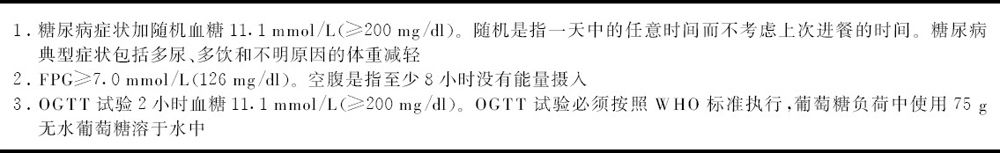
\includegraphics[width=5.90625in,height=3.02083in]{./images/Image00025.jpg}
\end{table}

\subsubsection{三、噬血细胞综合征(HPS)}

噬血细胞综合征是单核/巨噬系统反应性疾病,以组织细胞良性、大量增生,伴有明显的吞噬血细胞现象为特征。噬血综合征常常难以查出其病因,长期高热是噬血细胞综合征之一的表现,是由T细胞、巨噬细胞活化分泌IL-1、IL-6等内源性致热原而引起发热。

2004年国际组织细胞协会噬血细胞综合征的诊断标准:①发热,持续7天以上,体温超过38℃;②脾大;③全血细胞减少;④高甘油三酯血症或低纤维蛋白血症;⑤骨髓、脾、淋巴结中可见到吞噬红细胞、粒细胞或血小板的组织细胞;⑥NK细胞活性减低或缺失;⑦铁蛋白升高(铁蛋白≥3SD正常值,通常≥1000ng/ml);⑧可溶性IL-2受体(sCD\textsubscript{25}
)水平明显升高。8项中符合5项可考虑噬血细胞综合征。分遗传性和获得性,前者常发生于0~2岁的婴幼儿,后者可继发于感染(病毒尤其EB病毒、细菌、真菌、原虫)、淋巴瘤和自身免疫性疾病。其中EB病毒感染相关的噬血细胞综合征是长期不明发热的病因之一,包括EB病毒阳性的T淋巴细胞增殖症和淋巴瘤相关的噬血细胞综合征,前者血清EBV抗体滴度增高、EBDNA拷贝数升高,但淋巴结病理检查中未见典型的淋巴瘤表现,骨髓细胞也未检出克隆性T细胞受体重排。后者早期常常难以诊断,随病情进展组织活检有淋巴瘤的依据。

\subsubsection{四、急性白血病}

半数的患者以发热为早期表现。可低热,也可高达39~40℃以上,伴有畏寒、出汗等。外周血象初时有的仅有白细胞升高,红细胞、血小板数正常,易被考虑为感染性疾病。但动态观察红细胞、血小板可进行性下降。有的患者有不同程度的白血病细胞增殖浸润的表现如淋巴结肿大,肝、脾大、胸骨下段压痛,骨、关节疼痛,牙龈增生、肿胀,皮肤结节、斑块,中枢神经系统浸润的表现,睾丸浸润。血象:大多数患者白细胞增多,也有白血病数正常或减少,分类可见数量不等的原始及(或)幼稚细胞,有不同程度的正细胞性贫血,绝大多数患者血小板减少,常低于<20×10\textsuperscript{9}
/L。骨髓象是诊断急性白血病的主要依据。急性白血病患者的骨髓白血病性的原始细胞占骨髓有核细胞≥20\%。因此,凡遇有原因未明的发热伴有进行性贫血、出血者应行骨髓穿刺涂片检查以确诊。

有的患者血象呈全血细胞减少,无肝、脾、淋巴结肿大,需与急性再生障碍性贫血相鉴别。有的患者表现以出血为主,临床可与特发性血小板减少性紫癜相似,但后者以血小板减少为主,红细胞(出血严重者例外)与白细胞数不减少。

白细胞增多性急性白血病需与类白血病反应相鉴别(表\ref{tab2-20})。类白血病反应是机体受到较严重的病理损害时所发生的造血组织异常反应,其特征是外周血中白细胞数增多或(及)出现幼稚细胞,血象与白血病相似。病因以急性感染为多,其次为恶性肿瘤、急性溶血、中毒、大出血、结核病、寄生虫病等,按细胞类型可区分为中性粒细胞型、淋巴细胞型、单核细胞型、嗜酸性粒细胞型等。病因去除后类白血病反应即消除,有助于诊断。

\begin{table}[htbp]
\centering
\caption{类白血病反应与急性白血病鉴别}
\label{tab2-20}
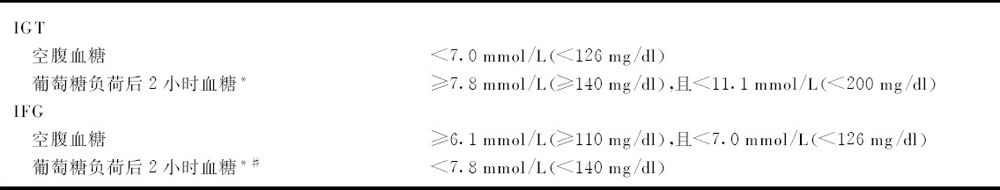
\includegraphics[width=5.91667in,height=3.875in]{./images/Image00026.jpg}
\end{table}

\subsubsection{五、组织细胞坏死性淋巴结炎}

组织细胞坏死性淋巴结炎,又称坏死性淋巴结炎、坏死增生性淋巴结病,是一种病因不明的非肿瘤性淋巴结肿大的疾病。

本病较少见,平均发病年龄30岁。起病急性或亚急性,特点如下:①95\%以上表现有发热:中、高度发热,热型呈不规则发热,也可呈弛张热,或反复间断发热,少数伴寒战,部分热程可长达2~3个月。②淋巴结肿大:多数有浅表淋巴结肿大以颈部最为常见,其次为腋窝及腹股沟,部分有压痛,也可有纵隔、腹膜后淋巴结肿大,少数有肝脾大。③少数有一过性皮疹、关节痛、多器官受累。④糖皮质激素治疗有效。

实验室检查:血象:白细胞计数常减少,可见核左移或异形淋巴细胞,轻度贫血,严重者血小板减少;对出现不明原因发热、浅表淋巴结肿大、白细胞减少,应想到本病的可能。淋巴结活检是本病诊断依据。病理学改变为淋巴结结构的部分或完全破坏,可见多少不等、大小不一的坏死灶,坏死灶周围组织细胞增多,坏死灶中可见浆细胞样单核细胞和免疫母细胞增生,无中性粒细胞浸润。由于本病的临床表现缺乏特异性,若未做淋巴结活检,误诊率高。本病需要与恶性淋巴瘤、结缔组织病、恶性组织细胞病、传染性单核细胞增多症相鉴别。

\subsubsection{六、Castleman病}

约近50\%的多中心型Castleman病表现为不明原因的长期发热,该病是一种少见的淋巴结增生性疾病,单中心型以纵隔、腹腔淋巴结肿大为多见;多中心型临床表现多样性、缺乏特异性,可以发热、浅表或深部淋巴结肿大,肝脾大,贫血,血小板减少,低白蛋白血症,免疫球蛋白升高(多克隆),易合并其他疾病或并发症如自身免疫疾病,POEMS,副肿瘤天疱疮,肾损害,淀粉样变。对疑诊本病,确诊需靠淋巴结活检病理检查,病理分为浆细胞型、透明血管型、混合型;临床分型包括单中心型、多中心型。

\subsubsection{七、朗格汉斯细胞组织细胞增生症}

一般多见于少儿,少见于成年人,临床表现:①发热:部分成年患者表现为长期发热、热型不规则,可呈周期性或持续性高热,使用抗生素无效,对激素敏感。②皮疹。③淋巴结肿大,肝、脾大。④肺部浸润:表现为轻重不等的呼吸道症状,但肺部体征不明显。肺部X线可见有弥漫性或网点状阴影。⑤骨骼破坏:长骨和扁平骨可发生溶骨性骨质破坏。⑥中枢神经系统:最常见的受累部位是丘脑-神经垂体区,弥漫性也可出现脑实质病变。有丘脑和垂体肉芽肿引起的尿崩症占该病的20\%~25\%。⑦其他:齿龈肿胀,牙齿松动,或突眼,或耳流脓或多饮多尿。病理检查是本病诊断依据,可行皮肤、淋巴结活检或病灶局部穿刺物病理检查。病理学特点是可见到特征性的分化较好的朗格汉斯组织细胞。该细胞CD1α、ATP酶、S-100蛋白、D-甘露糖苷酶均阳性。电镜下胞浆含有Birbeck颗粒。长期发热、尿崩症,要注意垂体朗格汉斯细胞组织细胞增生症。

\protect\hypertarget{text00035.html}{}{}

\subsection{5.3 风湿性疾病}

\subsubsection{一、成人斯蒂尔病}

成人斯蒂尔病(adult Still's
disease)是结缔组织病中引起长期不明原因发热的主要病因,占首位约50\%。成人Still病曾称为变异性亚败血症,是一种临床综合征。病因与发病机制尚未明确,可能与感染及自身免疫反应有关。发病年龄多于16~35岁,女性多见。表\ref{tab2-21}所示为文献报道的成人斯蒂尔病的主要临床表现。

\begin{table}[htbp]
\centering
\caption{成人斯蒂尔病的临床表现}
\label{tab2-21}
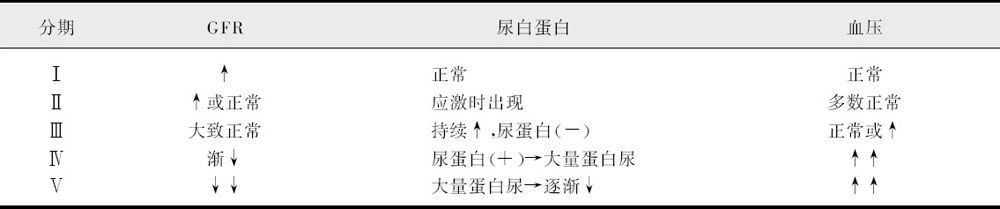
\includegraphics[width=5.9375in,height=2.29167in]{./images/Image00027.jpg}
\end{table}

\paragraph{1.临床特点}

\subparagraph{(1)发热:}

是本病的突出症状,多高于39℃,多数弛张热,也有不规则热,稽留热。热程1个月至1年,有报道平均5.3个月,常伴畏寒,但罕见有寒战,热程虽长,病情一般尚好,中毒症状不明显。各种抗生素治疗无效,而用糖皮质激素或非甾体类抗炎镇痛药能使体温降至正常。

\subparagraph{(2)皮疹:}

多为点状红疹,有时为斑丘疹或结节红斑,呈一过性,高热时出现,热退时消失。主要分布在躯干、四肢、手掌、足底。

\subparagraph{(3)关节痛或关节炎:}

可单关节或多关节受累。有时只有轻微关节痛。

\subparagraph{(4)其他:}

患者有咽痛,这是本病特征之一。部分有淋巴结肿大、肝脾大、胸膜炎、腹膜炎、心包炎、神经系统及呼吸系统损害等。除发热外有些患者起病时并非全部表现出上述症状,可能在病程中需要数月以至数年,才表现出来,亦可能始终未全部表现。

\paragraph{2.实验室检查}

(1)外周血白细胞总数增多,中性粒细胞核左移。

(2)血沉增快,C反应蛋白和免疫球蛋白升高。

(3)血清铁蛋白(SF)明显升高,铁蛋白>1000ng/ml(正常值上限的3倍)对诊断成人斯蒂尔病(AOSD)具有较高的阳性预测值(95.2\%),如果SF<1000ng/ml,则95.2\%认为不是AOSD;SF>1500ng/ml(正常值上限的5倍)阳性预测值为85.7\%,提示有临床表现者应高度怀疑AOSD。

(4)骨髓呈感染性骨髓象。

(5)2/3患者肝功能异常。

目前常用的诊断标准有日本成人Still病研究委员会制订的标准即Yamaguchi标准(1992):

主要指标:发热≥39℃,并持续1周以上;关节痛持续2周以上;典型皮疹;白细胞增高≥10×10\textsuperscript{9}
/L。

次要指标:咽喉痛;淋巴结肿大及(或)脾大;肝功能异常;类风湿因子和抗核抗体阴性。

符合5项条件含2项主要条件,排除感染性疾病及恶性肿瘤即可诊断。不典型的病例可无关节痛,一过性皮疹亦被疏漏。对于不典型病例必须充分排除其他引起长期发热的疾病才能诊断。

对诊为本病的患者必须长期随访,少数以后发展为淋巴瘤。

\subsubsection{二、系统性红斑狼疮}

长期的非感染性发热,兼有两个器官(如肾脏+浆膜;肾脏+关节;肝脏+心脏;关节+中枢神经系统)或多个器官受累的表现;发热伴血象白细胞减少、血小板减少、贫血或溶血性贫血者,应考虑系统性红斑狼疮(SLE)的可能。此病多见于女性,发病年龄多在21~40岁之间。以发热为主要临床表现者约占60\%~80\%。可以中、高热也可呈低热。首发症状的发热,伴皮疹与关节痛为多见。皮疹呈多形性,可从轻微的红斑乃至急性丹毒样病变或大疱,多见于面、颊、鼻、前胸、手、足等暴露处,但典型而有诊断价值的皮疹是蝶形红斑和盆状红斑。面部蝶形红斑虽为此病的特征性表现,但又非经常出现,国内报告阳性率为60\%~80\%。由于SLE症状复杂,如仅注意个别器官病变化,易误诊为风湿热、心包炎、胸膜炎、肾炎、类风湿关节炎、肝炎、特发性血小板减少性紫癜,甚至精神病等疾病。

美国风湿病学会1982年的SLE分类标准,对诊断SLE很有价值:①蝶形红斑:平的或高于皮肤的固定性红斑;②盘状红斑:面部的隆起红斑,上覆有鳞硝;③光过敏:日晒后皮肤过敏;④口腔溃疡;⑤关节炎:非侵蚀性关节炎;⑥浆膜炎:胸膜炎或心包炎;⑦肾病变:蛋白尿>0.5g/d或细胞管型;⑧神经系统病变:癫痫发作或精神症状;⑨血液系统异常:溶血性贫血或白细胞减少或淋巴细胞绝对值减少或血小板减少;⑩免疫学异常:狼疮细胞阳性或抗ds-DNA或抗Sm抗体阳性或梅毒血清试验假阳性
;\textcircled{11}
抗核抗体阳性。在上述11项中,如果有4项阳性,则可诊断为SLE,其特异性为98\%,敏感性为97\%。

SLE血清抗核抗体(ANA)是筛选结缔组织病的主要试验,阳性率达95\%~100\%,但特异性较差,其他结缔组织病、慢性活动性肝炎等均可呈阳性,诊断须结合临床与其他检查。血清抗双链去氧核糖核酸抗体(ds-DNA)特异性较高,且疾病早期即可出现,阳性率约62\%。抗Sm抗体是诊断SLE的标记抗体之一。特异性达99\%,但敏感性仅25\%。

系统性红斑狼疮样病象可由某些药物引起,称药物性狼疮综合征。可引起此综合征的药物可分为两类:①可引起红斑狼疮综合征的;②可使系统性红斑狼疮症状恶化的。属于第一类的药物有酰肼类药物(肼屈嗪、异烟肼等)、抗癫痫药物(如苯妥英钠)、普鲁卡因胺等。后者血清抗核抗体阳性率高达50\%~68\%,停药后症状在数周内消退,但血清抗核抗体阳性率可持续数月。此类药物性狼疮综合征罕有发生肾脏病变,且停药后不致再发。属于第二类的药物有青霉素、磺胺类、口服避孕药等,可使系统性红斑狼疮患者的症状恶化;但对正常人不致引起系统性红斑狼疮的病象或血清抗核抗体阳性。

\subsubsection{三、结节性多动脉炎(PAN)}

此病临床上少见,是一种累及中、小动脉的坏死性血管炎。此病的病理特点是多器官损害,主要累及心、肾、肺、肌肉、皮肤、关节等器官。患者以男性为多,年龄多在40~50岁之间,发热是最常见的症状,可高热也可低热。系统症状取决于受累器官。①皮肤表现:25\%~52\%患者有如血管性紫癜、结节红斑样皮肤结节、网状青斑、远段指(趾)缺血或坏死及雷诺现象;②关节肌肉表现:46\%~63\%患者可有关节炎、多发性肌痛和间歇性跛行;③神经系统表现:36\%~72\%患者有神经系统受累,以外周神经受累为主;④肾表现:45\%~83\%患者出现不同程度的肾损害,主要表现为蛋白尿,血、尿、细胞管型,高血压;⑤其他表现如胃肠道、心脏、肺、生殖系统等受累则有相应表现。

凡原因未明的长期发热,兼有多个互不相关的器官受累的表现,血象白细胞增多,须考虑此病的可能。实验室检查一般无特异性,可见轻度贫血、白细胞轻度升高,可见蛋白尿、血尿、管型尿,C反应蛋白增高,球蛋白升高,ANCA阴性,部分病例HBsAg阳性。诊断主要根据病理活检和血管造影。可行皮肤、肌肉、肾组织或睾丸活检。血管造影常见有肾、肝、肠系膜及其他内脏器官的中、小动脉有微小动脉瘤形成和节段性狭窄。1990年美国风湿病学会关于结节性多动脉炎的分类标准见表\ref{tab2-22},在10项中有3项阳性者排除其他结缔组织病并发的血管炎即可诊断。

此病在鉴别诊断上须多注意败血症、腹腔内恶性肿瘤、心肌炎、急性白血病、皮肌炎、系统性红斑狼疮、白塞病等疾病。

\subsubsection{四、肉芽肿性多血管炎(Wegener肉芽肿)}

Wegener肉芽肿是一种系统性、坏死性肉芽肿血管炎,主要累及上、下呼吸道及肾,同时也累及全身小动脉、静脉及毛细血管。本病临床上少见,无性别差异,以40~50岁为多见。

临床表现:①全身非特异症状如发热、关节痛、肌痛;②上呼吸道:表现为鼻、中耳、鼻窦的炎症;③肺部表现:肺病变见于70\%~80\%患者,可有咳嗽、咯血、胸痛和呼吸困难。X线示中下肺野结节和浸润或空洞;④肾病变:在病程中出现不同程度的肾小球性肾炎,重者可因进行性肾病变导致肾衰竭;⑤其他表现:部分有眼、皮肤、心脏受累的相应表现。

\begin{table}[htbp]
\centering
\caption{美国风湿病学会关于结节性多动脉炎的分类标准}
\label{tab2-22}
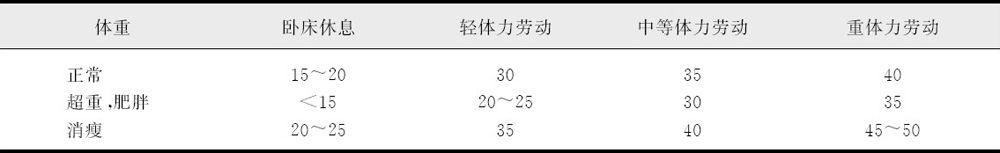
\includegraphics[width=5.91667in,height=3.03125in]{./images/Image00029.jpg}
\end{table}

实验室检查示:贫血、白细胞增多、血沉加快、类风湿因子低度阳性。血清中胞浆型抗中性粒细胞胞浆抗体(c-ANCA)阳性是诊断Wegener肉芽肿的重要参考指标。特异性为86\%,敏感性为78\%。

组织病理:鼻窦及鼻病变组织活检示坏死性肉芽肿及(或)血管炎。肾活检示局灶性节段坏死性肾小球肾炎。皮肤活检示白细胞破碎性血管炎。对临床表现有上、下呼吸道病变与肾小球肾炎者,实验室检查c-ANCA阳性,组织病理检查呈坏死性肉芽肿者可确诊。

此病与结节性多动脉炎的区别在于后者早期即出现肾脏损害,心脏通常明显受累。肺部症状主要为哮喘兼有嗜酸性粒细胞浸润和血中嗜酸性粒细胞增多等。此外还须与恶性中线性肉芽肿、特殊性传染性肉芽肿(结核性、梅毒性、真菌性等)、结节病、败血症、原发性肺癌等相鉴别。诊断主要依靠病理组织活检。

\subsubsection{五、混合性结缔组织病(MCTD)}

MCTD的特点为具有系统性红斑狼疮(SLE)、多发性肌炎、进行性系统性硬化、类风湿关节炎等多种结缔组织病的症状,肾脏损害轻。发热几乎经常出现。实验室检查显示高阳性率(达100\%)和高滴度的核糖核蛋白(RNP)抗体;荧光抗核抗体(FANA)达100\%阳性;而抗Sm抗体阴性,抗双链去氧核糖核酸抗体(ds-DNA)与狼疮细胞均呈低阳性率,C3、CH50均正常,提示MCTD是一种有特色的未分化结缔组织病。

\subsubsection{六、IgG4相关的硬化性疾病}

IgG4相关硬化性疾病是新近认识的一种疾病,是以累及胰腺以及胰腺外的肺间质,腮腺、泪腺、下颌腺等外分泌腺,胆道、后腹膜、肾脏、胃肠道、肝脏、乳腺等器官和脏器的慢性炎症性病变,血清学显示高γ球蛋白血症。病变部位以浆细胞浸润和纤维化为突出表现,可以检测到大量表达IgG4阳性的浆细胞,与自身免疫有关,且对类固醇激素治疗有效的一组异质性疾病。

患者可有不明原因发热、乏力、体重下降等全身表现,其他症状与受累器官组织有关,不同的器官组织受累有不同的表现,主要表现为局部压迫症状和相应腺体功能障碍。本病主要累及外分泌腺,多数患者胰腺受累,可表现为慢性轻中度腹痛、糖尿病。患者常因无痛性黄疸就诊,黄疸可呈波动性。涎腺、泪腺受累可出现腺体无痛性肿大,口眼干燥。此外,腹膜后纤维化的患者可出现腰背痛,因输尿管受压可能出现肾功能不全的表现。还有小管间质性肾炎、间质性肺炎、前列腺炎、乳腺炎等,症状均不特异。还可累及内分泌腺,包括垂体炎、Riedel甲状腺炎等。中枢神经系统受累很少见,但有硬脑膜、室管膜炎性假瘤和硬脑脊膜炎的报道。

多数患者出现高γ球蛋白血症,血清IgG、IgG4升高,IgG4/IgG比值升高,血清IgG4>1350mg/L对诊断AIP敏感性和特异性均很高,对诊断为AIP的患者,血清IgG>2200mg/L常提示胰腺外损害。

影像改变:累及胰腺时表现为胰腺弥漫性肿大,呈“腊肠样”,动态CT显示延迟强化。胰腺局灶性增大。内镜逆行胰胆管造影(ERCP)主胰管不规则狭窄,硬化性胆管炎患者胆管狭窄。肺部受累的CT表现主要分4型:实性结节型、圆形磨玻璃影型、肺泡间质型、支气管血管型。本病的肾损害主要在肾皮质,CT增强时表现为外围皮质圆形、楔形边界清楚的低密度影。

病理学组织淋巴浆细胞浸润、弥漫而致密的纤维化是这类疾病的特点;免疫组化显示,浸润的淋巴细胞主要是CD4\textsuperscript{+}
或CD8\textsuperscript{+} T细胞和IgG4\textsuperscript{+}
浆细胞,后者常超过30个/高倍镜。诊断依靠临床表现、血清学检查、影像学改变和病理学改变。

有报道一女性,56岁。不明原因发热3个月,腰痛1个月入院。胸部增强CT:后纵隔降主动脉周围软组织肿块,所示胸主动脉下段及腹主动脉旁不规则软组织影,包绕主动脉生长,下段腹主动脉旁及左侧髂总动脉旁不规则软组织影,包绕动脉生长,IgG
19.72g/L,IgG4:0.84g/L,行腹主动脉旁软组织活检术,病理:送检组织为大量增生纤维组织及脂肪和淋巴结一枚,淋巴结未见特殊病变,增生纤维组织中可见到大量浆细胞及中等量淋巴细胞,浆细胞浸润血管周隙及神经纤维束周围,酶标结果提示浸润淋巴细胞为CD4\textsuperscript{+}
T细胞,浆细胞分泌IgG为主,其中lgG4\textsuperscript{+}
细胞>20个/高倍视野,考虑IgG4相关硬化性疾病。

\protect\hypertarget{text00036.html}{}{}

\subsection{5.4 恶性肿瘤}

肿瘤性发热仅次于感染。恶性肿瘤患者长期发热见于两种情况:恶性肿瘤本身引起的发热和恶性肿瘤伴发感染所引起的发热。本处重点叙述肿瘤本身引起的发热。肿瘤热是由肿瘤细胞本身产生内源性致热因子,肿瘤迅速生长,瘤组织相对缺血、缺氧、坏死、出血引起吸收热;瘤组织坏死释放肿瘤坏死因子(TNF),TNF能诱导IL-1、IL-6的产生。TNF、IL-1、IL-6均为内源性致热原,而引起发热。

引起长期不明原因发热常见恶性实体瘤有原发性或继发性肝癌、肺癌、肾癌、甲状腺转移癌。较少见引起发热的有:结肠、卵巢、前列腺、乳腺、直肠、胰腺(无转移)和大脑恶性肿瘤、胃印戒细胞癌、松果体瘤、黑色素瘤、转移癌等。罕见引起发热的有嗜铬细胞瘤。此外,心房黏液瘤和胃、肾血管平滑肌脂肪瘤、小肠平滑肌瘤等是引起发热的良性肿瘤。

临床上,大多数恶性肿瘤引起的长期发热不超过38.9℃,如果超过此水平,一般提示感染性因素所致。热型多为弛张型或不规则型,患者通常无寒战,萘普生(naproxen)对肿瘤热有选择性解热作用。提示恶性肿瘤的其他症状是进行性消瘦、贫血等。对原因未明的低血糖状态、类白血病反应、游走性血栓性静脉炎、皮肌炎、纤维蛋白原缺乏症、红细胞增多症等情况,也须警惕恶性肿瘤的可能性;肾癌、肝癌、转移性肺癌、前列腺癌等,均可伴有红细胞增多症。癌也较常伴发于肺性肥大性骨关节病、皮肌炎、黑棘皮病等疾病。

肝癌:一些不典型或特殊表现的肝癌易被临床所忽视。肝大不明显,质不硬,甲胎蛋白反相间接血凝法或火箭电泳阴性,B超和CT有可能帮助发现本病,肝穿可找到确诊依据。

肾细胞癌很隐匿,约10\%的肾癌患者以发热为主要表现,通常仅表现为发热,无其他表现,有时伴乏力和消瘦,镜下血尿或血红细胞增多、血清碱性磷酸酶增高,可提示本病。B超、CT、选择性肾动脉造影有助于诊断。

嗜铬细胞瘤FUO,常见于发作性高血压病例,血压升高时体温增高,血压正常时体温降至正常。

肺癌通常不引起FUO,但部分病例在没有肺炎和肺不张的条件下表现为FUO。

心房黏液瘤可表现为发热、心脏杂音可呈现间隙性、体位性或缺如。血沉增快和贫血常见,超声心动图可确诊。

骨肉瘤也较常有发热的倾向。

\protect\hypertarget{text00037.html}{}{}

\subsection{5.5 中枢性发热}

下丘脑(间脑)综合征可由于炎症、肿瘤、外伤等引起,可导致长期不规则间歇发热,各项检查无急性感染的证据,血、尿培养均阴性,毒血症症状也不明显,应用各种抗生素而发热不能缓解。患者常伴有思睡、厌食或多食、肥胖、尿崩症、性功能减退以及自主神经功能紊乱症状等。

\protect\hypertarget{text00038.html}{}{}

\section{6 慢性低热}

体温上升达37.4~38℃(舌下测温)并除外生理性原因者称为低热;低热持续1个月以上者称为慢性低热。

有些高温作业的人、孕妇或女性排卵期,体温可较正常略高,但如离开高温环境或分娩后或排卵后,体温恢复正常,这种情况可称为生理性高体温,而非低热状态。

慢性低热可见于许多情况,一般可区分为器质性与功能性两大类(表\ref{tab2-23}),其中以器质性为常见;病因又以感染为多(表\ref{tab2-24})。

慢性低热的检查须注意下列情况:

\subsection{1.病史}

结核病史或结核患者接触史、咯血史、肝病史或黄疸史、局灶感染史、高温作业史等。

\subsection{2.体格检查}

需做全面体格检查,特别注意中耳炎、乳突炎、鼻窦炎、扁桃体炎、龋齿及齿根尖脓肿、前列腺炎等局灶性感染,贫血外貌,淋巴结与肝脾大,腹部压痛与包块,肾区叩击痛与压痛,脊柱压痛与纵轴叩击痛等。女性患者须考虑妇科检查。

\subsection{3.化验检查}

应作血、尿、便三项常规检查和血沉测定。未能除外感染或结缔组织病时,做抗链球菌溶血素“O”滴度测定、血清蛋白电泳测定、血中狼疮细胞检查,以及有关的血清免疫学检查。怀疑肝脏疾病时做常规肝功能试验。结核菌素试验强阳性有助于活动性结核病的诊断,但阴性未能排除此病。患者有未能解释的贫血时,须做骨髓象检查。

\begin{table}[htbp]
\centering
\caption{慢性低热疾病分类}
\label{tab2-23}
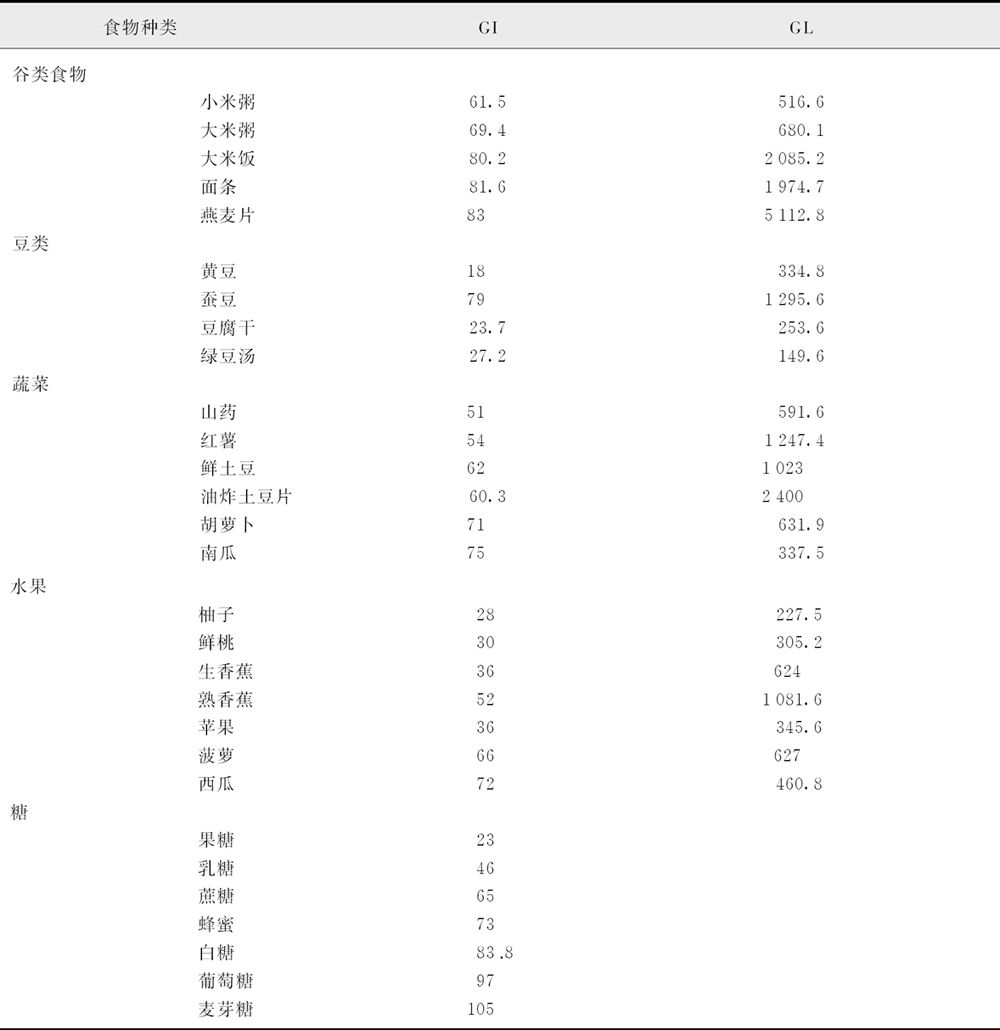
\includegraphics[width=5.875in,height=2.08333in]{./images/Image00030.jpg}
\end{table}

\begin{table}[htbp]
\centering
\caption{800例低热的原因分析}
\label{tab2-24}
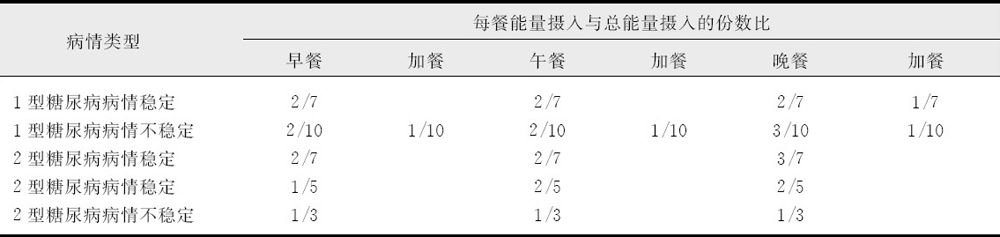
\includegraphics[width=6.03125in,height=6.08333in]{./images/Image00031.jpg}
\end{table}

\subsection{4.器械检查}

X线胸部透视应作为常规检查,需要时摄片。心电图描记、甲状腺吸131碘试验、超声肝区检查、胃肠钡餐透视与钡剂灌肠、眼底检查等,可按需要选择行之。未除外胆道感染者,有指征作十二指肠引流及(或)胆囊造影检查。疑为胸腹占位性变时做B超与CT检查。

\protect\hypertarget{text00039.html}{}{}

\subsection{6.1 器质性慢性低热}

\subsubsection{6.1.1 感染性慢性低热疾病}

\paragraph{一、结核病}

患者有慢性低热与结核中毒症状时,首先应考虑结核病。最常见的是肺结核,但早期可无呼吸系统症状与体征,X线透视检查也不一定完全可靠。有怀疑时应做胸部照片检查。

诊断困难者为肺外结核。肺外结核种类繁多,包括多系统、多脏器、多部位、多种类型的结核性病变。诊断比肺结核明显困难。为了避免误诊或漏诊,须注意:①进行全面、细致地病史询问和体检;②深部结核病灶或隐性病灶须选择X线、B超、CT、纤维内镜,甚至开腹探查协助诊断,从病理活检中确定诊断;③结核菌素试验;④如未排除隐性病灶的存在应采取积极的有效抗结核诊断性治疗,疗程不少于4~6周。由于近年来结核病有复燃之势,诊断性治疗临床症状奏效之后,对疑似病例仍需继续正规治疗,不能半途而废。

诊断上较难的肺外结核病变,如肾结核大多数发生于20~40岁之间,主要症状不表现于肾而表现于膀胱,约75\%~85\%患者有膀胱刺激征,如尿频、尿急与尿痛。主要化验所见为血尿,多为镜下血尿,有时为肉眼血尿,常间歇出现。其他症状为低热、腰痛、纳差、盗汗、消瘦、倦怠等。

肝结核少见,也可引起慢性低热,结核菌素试验阴性不能除外此病,临床上不易诊断。CT扫描有助于发现粟粒病灶。

骨结核主要侵犯儿童与年轻成人。骨结核好发于脊椎,最常侵犯腰椎或胸椎,易于漏诊,腰背部局限性隐痛及(或)固定性局限性脊椎压痛提示此病的诊断。

肠系膜淋巴结结核,主要侵犯儿童与青少年,常与肠结核及结核性腹膜炎并发。凡年轻患者有原因未明的慢性发热与结核中毒症状、血沉加快、营养不良及与饮食无关的腹痛,即使腹部未触及包块,也须考虑腹腔内淋巴结结核的可能性,结核菌素试验强阳性(但阴性未能除外本病)和腹部X线摄片发现钙化灶,有力地支持本病。抗结核药物诊断性治疗奏效时可证实临床诊断。本病往往须手术探查方能明确诊断。

女性生殖器结核,主要侵犯附属器官,症状不典型,临床诊断不易。发病多在20~40岁之间,往往有低热、倦怠、下腹痛、盗汗、体重减轻等症状。妇科病征则有月经稀少,闭经与不育。遇见女性结核患者,尤其是肺结核病或腹膜结核,或患者有全身性结核病症状而找不到病灶,而同时有不育症,月经稀少或闭经,应考虑女性生殖器结核的可能性。

肾上腺结核少见,此病临床上往往表现为Addison病。国内一组3例原发病为肺结核,肾上腺结核均经CT证实。

\paragraph{二、慢性非特异性局灶性感染}

扁桃体、齿根、鼻窦、中耳、乳突、胆道、肠道、肾盂、前列腺、女性内生殖器等处的慢性炎症,也有引起慢性低热的可能,但以不规则的波动性发热为多见。患者除局部病征之外,并常有精神体力欠佳、血沉轻度加快等表现。有的患者伴有心悸、多汗、皮肤划痕症等自主神经功能紊乱症状。局灶性感染根治后,低热及其他症状也随之消退。

链球菌感染后状态:临床上可见到一些扁桃体炎或咽炎之后出现低热、关节酸痛。心率加快、抗“O”增高,血沉正常或轻度加快,咽拭子培养可证明乙型溶血性链球菌,心电图检查可发现短暂的期前收缩或(及)轻度S-T段与T波改变。无心脏增大与心杂音。给予青霉素或其他抗菌药物治疗,常于短期内解热。关节痛及其他症状均消失;如病情改善不明显,加用小剂量泼尼松也奏效。这种情况可称为链球菌感染后状态,如经上述治疗病情仍无好转或有再发,须考虑为风湿热或其他并存的疾病。

\paragraph{三、慢性病毒性肝炎}

慢性无黄疸型病毒性肝炎可引起低热。患者除有食欲减退、肝区隐痛、肝大压痛等肝炎表现外,常兼有多汗、易兴奋、失眠等自主神经功能紊乱症状。低热于休息时较低,活动或劳累略有升高,热程可累月甚至经年。患者肝功能多有异常,还可在血清中检出特异性肝炎标志物。十二指肠引流有时可发现“B”、“C”管的胆汁中白细胞数增加,容易与胆道感染相混淆。胆汁培养无细菌生长,镜检无寄生虫发现,诊断性治疗不奏效,据此可与慢性胆道感染相区别。

\paragraph{四、巨细胞病毒感染}

近年有人注意到巨细胞病毒感染所致的持续微热状态。这种病毒感染又称为全身性巨细胞性包涵体病,其临床表现变异很大。可表现为类似传染性单核细胞增多症的综合征,但嗜异性凝集反应阴性。也可引起慢性肝脏病变。表现为慢性无黄疸型肝炎。诊断须依靠血、尿的病毒分离培养,巨细胞病毒补体结合试验,尿路上皮细胞中发现细胞核内包涵体等。

\paragraph{五、梅 毒}

梅毒第二期以后的表现较为复杂。如患者有梅毒接触史,血清梅毒抗体特异性试验阳性,而有原因未明的慢性低热,应考虑此病的可能性。

\paragraph{六、艾滋病}

艾滋病亦可表现为慢性低热。

\paragraph{七、其 他}

也见有个案报道布鲁杆菌病、伤寒、POEMS、恶性间叶瘤也可引起低热。

\protect\hypertarget{text00040.html}{}{}

\subsubsection{6.1.2 非感染性慢性低热疾病}

\paragraph{一、甲状腺疾病}

甲状腺功能亢进、甲亢危象,亚急性甲状腺炎、甲状腺癌中滤泡细胞型者、少数桥本病表现为亚急性甲状腺炎或甲亢,均可有不同程度发热和出汗,这些患者发热同时多有高代谢症候群。

\paragraph{二、风湿性疾病}

风湿性疾病以发热为主要临床表现,因此呈慢性低热者亦有之。这种情况可见于风湿热、系统性红斑狼疮、结节性多动脉炎、皮肌炎,结节病、大动脉炎、小血管炎也见有个案报道表现为低热。

\paragraph{三、肝硬化}

肝硬化患者约1/4~1/3有发热,大多由于肝细胞坏死或肝内炎症等活动性病变所致。部分病例呈低热,常未能发现任何发热的原因。发热较高时往往提示合并感染。

\paragraph{四、炎症性肠病}

Crohn病及溃疡性结肠炎,均可有慢性低热,提示轻度的炎症活动。

\paragraph{五、失代偿性心瓣膜病}

失代偿性心瓣膜病可能有持续的低热,由于淤血性支气管炎、细小的肺梗塞或血栓性静脉炎等所致。或认为在充血性心力衰竭时,由于心排血量降低、皮肤血流量减少以及水肿的隔热作用,使散热减少,再由于呼吸困难时呼吸肌运动量增加,使热的产生有所增加,故可有低热。

如患者持续低热兼有关节(肿)痛,心律失常如心房颤动、阵发性心动过速、期前收缩的出现,洋地黄耐受量降低,新的瓣膜病变杂音的出现或心杂音的改变(包括强度增加与音质改变)等情况,则应考虑活动性风湿性心脏病。如持续低热兼有栓塞现象(皮肤或结膜瘀点),则提示并发亚急性细菌性心内膜炎的可能性。

\paragraph{六、血液病}

重症贫血患者常有低热,乃由于基础代谢率稍有增高之故。慢性白血病与恶性淋巴瘤也可有低热。少见病Castleman病也可以长期低热。

有报道:男,34岁,反复午后低热11年,37.2~37.5℃,浅表淋巴结肿大,最大直径2cm,病初淋巴结活检示淋巴结反应性增生,短期糖皮质激素治疗淋巴结有缩小,但仍反复低热,11年后除了浅表淋巴结肿大外、肝脾大,白细胞低、小细胞低色素性贫血;高球蛋白血症,多克隆性免疫球蛋白及轻链升高;PT、APTT延长,反应性浆细胞增多。低氧血症,双肺弥漫性病变,蛋白尿,镜下血尿,B超示双肾弥慢性病,淋巴结活检示Castleman病。

\paragraph{七、恶性肿瘤}

恶性肿瘤有发热的倾向,特别是肺癌、肝癌、结肠直肠癌。低热一般见于无并发症和无进行性急剧坏死的恶性肿瘤。中年以上患者有慢性低热与血沉加快,虽无任何其他病征,也须注意深部恶性肿瘤的可能性。

\paragraph{八、间脑(下丘脑)综合征}

间脑由丘脑、丘脑底、下丘脑和第三脑室周围结构所组成,是大脑皮质和各低级部位相互联系的重要机构。间脑综合征较下丘脑综合征有更广的范围,二者都可引起体温调节障碍,以及一系列自主神经失调症状,症状还有发作性的特点。

下视丘视前区两侧急性病变常引起体温迅速升高;慢性起病的间脑综合征则不少有低热。发病以21~40岁为多。据我院1963年总结30例的经验,病因以感染为多,其次为脑外伤、肿瘤、中毒等,但也有原因未明者。

间脑功能十分复杂,间脑病损主要有下列表现:

\subparagraph{1.自主神经功能紊乱症状}

如多汗或无汗;多尿或少尿,脉快或脉慢,血压升高或降低,发作性头昏,皮肤划痕症等。此外尚可表现为半侧感觉障碍、半侧水肿。半侧皮肤发红、半侧无汗或多汗等。

\subparagraph{2.内分泌代谢障碍}

如肥胖,糖耐量曲线异常,剧烈饥饿感、皮肤不对称性水肿,性欲减退,月经不正常,不育等。

\subparagraph{3.睡眠障碍}

如嗜睡或失眠,倒错性睡眠(白天嗜睡,夜间不睡)。

\subparagraph{4.体温调节障碍}

以慢性低热最为多见。低热的特点是:①对解热药呈异常反应;非间脑病变时,服阿司匹林后开始时皮肤温度升高,而在间脑病变时呈倒错反应(即开始时皮温下降)或无反应。②两半侧身体皮肤温度不对称现象,在间脑病变时相差甚明显,如相差在0.4~
0.5℃时可认为是病理性。③24小时体温曲线正常人在下午较高,连续测量数天在间脑病变有时上午较高。

间脑综合征的诊断主要根据:①有关的既往病史;②在短期内出现上述大部分症状;③症状分布为全身性或半侧性;④有发作性的特点;⑤脑电图各导联阵发性出现θ波有助于诊断。其病因的诊断较难,必须联系下丘脑的生理功能,结合有关下丘脑靶腺反馈机制,头颅CT和磁共振等影像学特征作出诊断。

\paragraph{九、更年期症候群}

更年期症状与体征均与雌激素水平下降有关,常见症状为阵发性潮红,尤其面颈部皮肤多见,可持续数年,其次为发热和出汗,也多有阵发性规律,感觉异常,手脚发凉,头晕头痛、失眠,健忘,精力不集中,精神紧张,焦虑,神经质等更为多见,血浆雌二醇及孕酮降低,促卵刺激素升高,促黄体生成素多正常,结合年龄和闭经史诊断较易。

\protect\hypertarget{text00041.html}{}{}

\subsection{6.2 功能性低热}

功能性低热的临床特征是患者体温较正常人升高约0.3~0.5℃左右,一般不超过38℃。经反复体检,病理学和实验室检查,除体温升高外未见其他异常,长期观察,一般情况良好,不影响正常工作和生活,经抗感染、抗结核、抗风湿等治疗无效。

\subsubsection{一、感染后低热}

在其前往往有细菌、病毒、衣原体、原虫等感染,特别多见于病毒感染后。此时体温调节中枢对体温的调节功能仍未恢复正常所致。

\subsubsection{二、手术后低热}

手术后可以有术后吸收热,一般在术后6~8小时开始发热,持续3~5天可自行缓解,但部分患者低热持续,而与手术相关的切口等均正常。

\subsubsection{三、功能性低热}

多见于青年女性,为一种原发性低热,日间温差不大(相差0.5℃左右),体温昼夜规律失常。晨间午前往往较下午晚间略高,体力活动体温可不升或有时反而下降。持续数月、数年,体温往往在偶然或患者不注意情况下自动下降。患者又常兼有多汗、手颤、皮肤划痕症、呼吸性不整脉、怕冷、心悸、失眠等自主神经功能紊乱的表现。

\subsubsection{四、夏季低热}

低热仅发生于夏季,秋凉后自行退热,每年如此反复出现,连续数年后多可自愈。多见于幼儿,因体温调节功能不完善,夏季身体虚弱,且多发生于营养不良或脑发育不全者。

\subsubsection{五、其 他}

妊娠初期也可有低热现象。部分妇女月经前7~10天体温上升至37.5℃,月经来潮后体温降至正常。

功能性低热的诊断需根据较长时间的观察,排除各种器质性疾病,如肺外结核、甲亢、恶性肿瘤,在女性尤需注意卵巢癌,男性患者诊断功能性低热需慎重。

\protect\hypertarget{text00042.html}{}{}

\section{参考文献}

1.胥婕,等.北京地区250例严重急性呼吸综合征患者临床分析.中华结核和呼吸杂志,2003,26(11):683-685

2.倪安平.衣原体的肺部感染.中华结核和呼吸杂志,1998,21(9):516-517

3.李丽,等.鹦鹉热衣原体肺炎一例.中华结核和呼吸杂志,1999,22(11):662

4.刘忠达,等.恙虫病肺部合并症50例临床分析.中华结核和呼吸杂志,2002,25(8):478-480.

5.陈晓红.恙虫病致肺损害46例.中华传染病杂志,2002,20(5):312-313

6.张溪林,等.恙虫病致急性肺损伤/急性呼吸窘迫综合征.中华传染病杂志,2003,21(6):436-437

7.黄学焕,等.96例肺下叶结核的诊断与鉴别诊断.中华内科杂志,1994,33(8):515

8.梁思礼,等.类鼻疽肺病四例报告与文献复习.中华结核和呼吸杂志,1994,17(3):168-170

9.陆慰萱,等.嗜肺军团杆菌肺炎37例综合分析.中华结核和呼吸杂志,1997,20(2):91-94

10.张斌,等.变态反应性支气管肺曲霉病.中华结核和呼吸杂志,1999,22(6):377-378

11.文仲光,等.肺毛霉病------附二例报告.中华内科杂志,1998,37(5):327-329

12.张可,等.艾滋病合并卡氏肺孢子虫肺炎的临床特点及诊断方法.中华结核和呼吸杂志,2002,25(8):475-477

13.金明根,等.生食鳖所致比翼线虫病的临床分析.中华结核和呼吸杂志,1998,21(10):611

14.燕航,等.肾移植术后巨细胞病毒肺炎的诊治.中华器官移植杂志,2001,22(5):298-300

15.徐志松,等.异基因骨髓移植后巨细胞病毒肺炎的临床研究.中华结核和呼吸杂志,2004,27(9):646-647

16.徐小元,等.人禽流感的流行病学与生物学.中华医学杂志,2004,84(5):353-354

17.林江涛.人禽流感的诊断治疗策略.中华医学杂志,2004,84(5):355-356

18.刘又宁,等.中国城市成人社区获得性肺炎665例病原学多中心调查.中华结核和呼吸杂志,2006,29:3-8

19.中华医学会呼吸病学分会感染学组.肺真菌病诊断和治疗专家共识.中华结核和呼吸杂志,2007,30:821-834

20.唐可京,等.肺接合菌的诊治.中华结核和呼吸杂志,2009,32:793-796

21.Gupta SK,et al.Evaluation of the Winthrop-University Hospital
criteria to identify Legionella pneumonia. Chest.2001,120(4):1064-71

22.Agarwal R,et al.Aspergillus hypersensitivity in patients with
chronic obstructive pulmonary disease:COPD as a risk factor for
ABPA?Med Mycol.2010,48:988-994

23.中华人民共和国国家卫生和计划生育委员会.人感染H7N9禽流感诊疗方案(2013年第2版).中华临床感染病杂志,2013,6(2):65-67

24.韩明锋,等.国内102例人感染H7N9禽流感特点初步分析.传染病信息,2013,26(2):68-70

25.权菊香,等.2013年我国H7N9型禽病毒流感分析.中国临床药理学杂志,2013,29(6):426-428

26.杨钧,等.甲型H1N1流感合并肺炎的影像表现.中华放射学杂志,2010,44(2):119-122

27.陈枫,等.重症及危重症甲型H1N1流感肺炎的影像表现.中华放射学杂志,2010,44(2):123-126

28.罗宏,等.新型甲型H1N1流感重症患者肺部影像学变化及临床特点.中华结核和呼吸杂志,2010,33(6):415-418

29.Fujitani S,et al.Pneumonia due to Pseudomonas
aeruginosa:partⅠ:epidemiology,clinical diagnosis,and
source.Chest,2011,139(4):909-919

30.廖纪萍,等.军团菌肺炎的临床诊治进展.国际呼吸杂志,2007,27(21):1632-1636

31.姚郁林,等.肺出血型钩端螺旋体病113例X线诊断体会.山东医药,2008,48(25):47

32.刘又宁,等.中国1998年至2007年临床确诊的肺真菌病患者的多中心回顾性调查.中华结核和呼吸杂志,2011,34(2):86-90

33.姚婉贞.侵袭性肺曲霉病的诊断与治疗.中华结核和呼吸杂志,2011,30(11):812-814

34.何礼贤,等.慢性阻塞性肺疾病合并侵袭性肺曲霉病的病理生理特点及其诊断策略.中国真菌学杂志,2011,6(5):257-260

35.何礼贤.肺孢子菌肺炎的诊断与治疗.中华结核和呼吸杂志,2007,30(11):802-805

36.张波.急性间质性肺炎的诊断与治疗.上海医学,2009,32(10):843-844

37.庄谊.隐源性和继发性机化性肺炎临床和影像学特点分析.实用临床医药杂志,2011,15(19):147-149

38.降钙素原急诊临床应用专家共识组.降钙素原急诊临床应用的专家共识.中华急诊医学杂志,2012,21
(9):944-951

39.蔡闯,等.2009年甲型H1N1流感研究近况.中国急救医学,2009,29(6):553-555

40.权菊香,等.2013年我国H7N9型禽病毒流感分析.中国临床药理学杂志,2013,29(6):426-428

41.谢正德.儿童EB病毒传染性单核细胞增多症临床特征及诊断标准.实用儿科临床杂志,2007,22(22):1759-1760

42.林特夫,等.细菌L型感染的意义和研究进展.蚌埠医学院学报,2006,31(2):111-115

43.童强,等.肾移植术后巨细胞病毒性肺炎的诊断与治疗.解放军医学杂志,2006,31(7):716-771

44.倪莲芳,等.组织细胞坏死性淋巴结炎68例临床分析.中华医学杂志,2010,90:3147-3149

45.谭明旗,等.组织细胞性坏死性淋巴结炎48例临床分析.中国实用内科杂志,2003,23(1):51

46.刘本似,等.我国西藏地区兔热病(土拉菌病)14例报告.流行病防治研究,1974,(3):224

47.何远学.钩端螺旋体病26例临床分析.中国热带医学,2006,6(10):1830

48.林瑞炮,等.凶险型恶性疟疾临床分型及治疗.中华传染病杂志,2002,20(5):317

49.郑德福,等.1964-2011年中国大陆人体旋毛虫病流行分析.寄生虫病与感染性疾病,2011,9(3):119

50.李兴福,等.急性风湿热诊断的相关问题.临床内科杂志,2005,22(10):652

51.赵丹,等.登革热预警技术研究进展.中华流行病学杂志,2012,33(5):540

52.张顺先,等.我国2005~2012年登革热流行特征分析.中国医药指南,2013,11(16):401

53.罗雷,等.广州市1978至2006年登革热流行病学特征分析.中华传染病杂志,2008,26(8):490

54.查震球,等.175例恙虫病病例的临床和流行病学特征研究.中华疾病控制杂志,2010,14(8):720

55.张萌,等.中国恙虫病流行态势及预防控制.中华流行病学杂志,2011,32(4):419

56.杨晴,等.恙虫病临床特点分析.中华实验和临床感染病杂志(电子版),2011,5(1):42

57.胡相,等.一起人的类丹毒流行病学调查.中华预防医学杂志,1980,14(4):213

58.黄奕江.类鼻疽病的诊断与治疗.临床内科杂志,2010,27(8):512

59.林容,等.类鼻疽病122例临床特征及耐药性分析.广东医学,2011,32(17):2303-2304

60.杨柳,等.Lyme病的临床分析及诊断探讨.中国实用眼科杂志,2000,18(11):712

61.张清安,等.皮肌炎与多发性肌炎73例临床分析.中国实用内科杂志,2005,25(4):354

62.曾泉.变应性血管炎82例临床分析.中国医药指南,2013,11(16):238

63.虞瑞尧.发疹性传染病与药疹的诊断、鉴别诊断与治疗.传染病信息,2007,20(1):23

64.王红兵,等.成人变应性亚败血症8例临床分析.中国麻风皮肤病杂志,2006,22(2):173

65.马科,等.不明原因发热15年临床变迁.中华医院感染学杂志,2008,18(9):1279

66.陈志海,等.北京地区肾综出血热96例临床特征分析.中华内科杂志,2003,42(1):70

67.娄秀芬,等.感染性心内膜炎120例临床分析.中华内科杂志,2009,48(1):35-38

68.谢旭晶,等.近十年风湿热的演变.中华风湿病学杂志,2009,13(7):467

69.刘正印,等.药物热40例临床分析.中国实用内科杂志,2000,20(6):364-365

70.孟卉秦,等.麻疹145例临床分析.中国实用内科杂志,2002,22(5):300-301

71.王南,等.风疹118例流行特点及临床分析.中国实用内科杂志,2003(23):754

72.张小河.恙虫病诊治探讨.医药论坛杂志,2009,30(5):27

73.韩秀萍,等.皮肌炎、多发性肌炎52例临床分析.中国实用内科杂志,2004(24):430

74.陈林囡,等.成人斯蒂病的临床表现和治疗探讨.中国风湿病学杂志,2002,6(6):173-174

75.阮力,等.特殊首发表现的急性白血病20例误诊分析.中国实用内科杂志,2004,24(6):374-376

76.唐井钢,等.98例不明原因长期发热病因分析.中国现代医学杂志,2008,15:2258-2259

77.陈珺秋.系统性红斑狼疮38例临床分析.中外医学研究,2012,30:141-142

78.左晓霞.结缔组织病与发热.中国感染控制杂志,2009,05:297-300

79.中华医学会风湿病学分会.结节性多动脉炎.中华风湿病学杂志,2004,8(7):436-437

80.段新旺,等.韦格纳肉芽肿病34例临床分析.中华急诊医学杂志,2012,21(10):1159-1163

81.张国华,等.韦格纳肉芽肿病100例临床分析.中华风湿病学杂志,2010,14(10):677-681

82.中华医学会风湿病学分会.韦格纳肉芽肿病诊断和治疗指南.中华风湿病学杂志,2011,15(3):194-196

83.林果为.提高对长期发热为主要表现恶性淋巴瘤的诊断水平.上海医学,2002,25(3):133

84.姚秋菊,等.不明原因发热103例病因分析.中华传染病杂志,2003,21(6):427

85.韩红,等.成人不明原因发热急诊的临床研究.中华急诊医学杂志,2010,19(6):647-649

86.马小军,等.不明原因发热449例临床分析.中华内科杂志,2004,43(9):682-685

87.林昌锋,等.原因不明发热者122例分析.中国误诊学杂志,2011,35:8707-8708

88.江红,等.原因不明发热患者128例临床分析.中华传染病杂志,2007,10:621-623

89.侍效春,等.综合医院以不明原因发热为表现的结核病100例临床分析,中华内科杂志,2010,49(12),1002-1004

90.马科,等.不明原因发热15年临床变迁.中华医院感染学杂志,2008,18(9):1279-1281

91.楼国春,等.钩虫病致周期性发热一例.中华内科杂志,2004,43(8):632

92.牟向东,等.肺黏膜相关淋巴组织型边缘区B细胞淋巴瘤一例.北京大学学报(医学版),2007,39(4):346-350

93.王孝勤.回归热误诊一例.临床误诊误治,2004,17(1):72

94.喻艳林,等.10例人粒细胞无形体病暴发流行报告.中华传染病杂志,2010,28(3):168-170

95.谭阳,等.周期性发热综合征.中国实用儿科杂志,2004,19(1):51-54

96.雷玲田,等.脂膜炎患者的临床特征及治疗随访分析.中华风湿病学杂志,2009,13(1):36-38

97.李龙芸,等.124例疑难发热病的诊断.中华内科杂志,2000,39(5):323

98.朴雪梅,等.IgG4相关的硬化性疾病一例.中华风湿病学杂志,2010,14(11):790-791

99.黄晓燕,等.IgG4相关硬化性疾病.中华内科杂志,2010,49(10):891-893

100.罗金梅,等.第115例------全身淋巴结肿大、低热伴活动后气短.中华结核和呼吸杂志,2011,34(8):631-633

101.田瑛,等.以不明原因发热就诊的肿瘤患者42例临床分析.中华内科杂志,2010,41(11):727-728

102.翁心华,等.原因不明发热的病因诊断与合理治疗.中华内科杂志,2003,42(4):269-270

103.卢洪洲,等.原因不明发热142例病因分析.中华内科杂志,2005,44(6):466-468

104.Henter JI,et al.HLH-2004:Diagnostic and therapeutic guidelines for
hemophagocytic lymphohistiocytosis.Pediatr B1ood
Cancer.2007,48:124-131

105.李剑,等.不明原因发热为首发表现的淋巴瘤53例临床分析.中华内科杂志,2006,45(8):665-667

106.北京朝阳医院内科.800例低热患者临床分析.中华医学杂志,1975,55:331

\protect\hypertarget{text00043.html}{}{}


\chapter{呼吸困难}

呼吸困难是指患者主观上有空气不足或呼吸费力的感觉,而客观上表现为呼吸频率、深度(如呼吸速而浅或慢而深)和节律的改变。患者用力呼吸,可见辅助呼吸肌参与呼吸运动,严重者可呈端坐呼吸及发绀。

根据主要的发病机制,可将呼吸困难区分为下列五种基本类型。能引起呼吸困难的疾病繁多,见表\ref{tab3-1}。

\begin{table}[htbp]
\centering
\caption{呼吸困难疾病的分类}
\label{tab3-1}
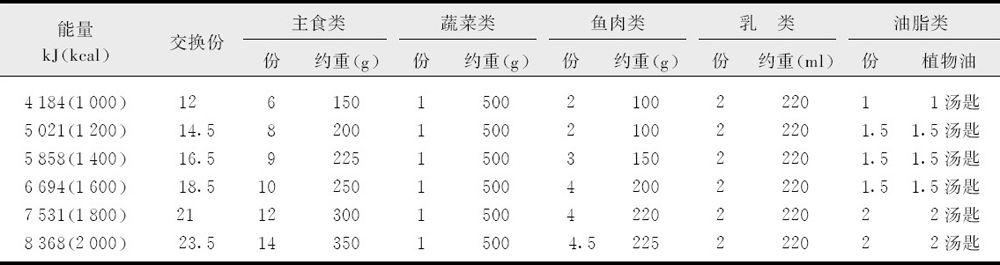
\includegraphics[width=5.95833in,height=5in]{./images/Image00032.jpg}
\end{table}

根据呼吸困难发生的缓急和伴随症状,可对呼吸困难作出初步的鉴别诊断:

\section{【急性发生的呼吸困难】}

1.时间超过1~2小时,伴有喘息者 支气管哮喘(病史可参考)、左心功能衰竭(心肌梗死、瓣膜病等)。

2.时间超过数小时/数天,伴有发热,有痰或无痰者 肺炎、急性支气管炎、急性胸膜炎、急性化脓性纵隔炎、急性心包炎等疾病。

3.高通气伴有代谢性酸中毒者 须考虑肾衰竭、糖尿病酮症酸中毒;有中毒者多为水杨酸盐、甲醇等。高通气综合征多为无心肺疾病的年轻女性。

4.呼吸困难同时伴有胸痛者 多为气胸(有气管移位)、肺栓塞(多有下肢静脉血栓,可有休克)、大叶性肺炎、急性心肌梗死、急性心包炎、急性胸膜炎、气道异物等。

5.产妇破水后突然出现呼吸困难、发绀、休克,应考虑为肺羊水栓塞症。长骨骨折后发生呼吸困难,须考虑肺脂肪栓塞。胸、腹大手术后突发呼吸困难,须考虑胸腔积液或肺不张。

\section{【慢性发生的呼吸困难】}

1.伴有胸膜炎性胸痛应注意胸腔积液、叶性肺不张、气胸、肺炎和肺栓塞等。

2.伴有大量脓性痰者多为支气管扩张,小量脓性痰可见于慢性支气管炎、支气管哮喘和肺炎。大量粉红色泡沫痰则见于急性左心功能不全,但也可见于肺泡细胞癌。

3.伴有咯血者如胸部X线检查显示中央气道异常可能是肺癌,胸部X线检查正常则可能为肺栓塞或肺血管炎(如Goodpasture综合征、多发性动脉炎)。

4.伴有全身衰弱者应注意神经肌肉疾病,如重症肌无力和运动神经元疾病。

\section{【如何评价呼吸困难】}

\subsection{(一)病史}

心、肺、胃肠病及肾脏病史,以往气喘发作史及诊疗经过,内因性与外因性中毒,职业性粉尘或异物吸入史,过敏病史,用药史,高原居留史。

病史询问应了解下列问题:①呼吸困难是突然发生还是逐渐发生?②患者的年龄,以及症状缓解和恶化的特点?③是休息还是活动时出现呼吸困难?④出现呼吸困难症状时的活动程度如何?临床上常用改良的呼吸困难分级量表(modified
Medical Research Council dyspnoea
scale,mMRC)评估呼吸困难程度,特别适用于慢性支气管炎和慢性阻塞性肺疾病患者。mMRC分为0~4级共5个级别,级别越高,患者呼吸困难越重:其中0级表示患者仅在费力运动时出现呼吸困难;4级表示患者因严重呼吸困难不能离开家,或在脱/穿衣服时出现呼吸困难。急性呼吸困难常常导致严重的后果,需要立刻评估和治疗(表\ref{tab3-2})。

\begin{table}[htbp]
\centering
\caption{呼吸困难程度}
\label{tab3-2}
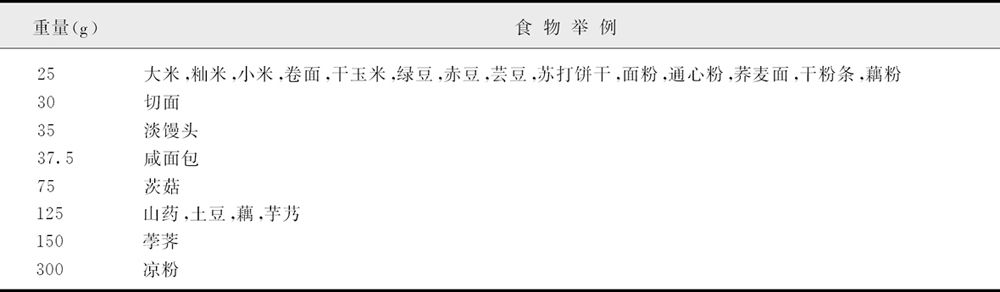
\includegraphics[width=5.90625in,height=1.39583in]{./images/Image00033.jpg}
\end{table}

\subsection{(二)体检}

咽、喉与胸部体征,肝脾大,腹水、水肿。肺部是体检的重点。另外还需评估患者的心脏情况,排除心脏疾病。

\subsection{(三)化验检查}

血象,嗜酸性粒细胞计数,有指征时作血尿素氮、血糖测定、动脉血气分析与酸碱度测定、痰检查(包括痰涂片找抗酸杆菌、痰培养和痰的细胞学分析等)。

\subsection{(四)器械检查}

X线胸部透视或(及)摄片;有指征时作静脉压测定、血循环时间测定、心电图描记、肺功能检查、放射性核素肺扫描、CT、纤维支气管镜检查、肺血管造影等。

\protect\hypertarget{text00044.html}{}{}

\section{7 肺源性呼吸困难}

广义的肺源性呼吸困难是由于呼吸器官(包括上呼吸道、支气管、肺、胸膜)病变、纵隔病变、胸廓运动以及呼吸肌功能障碍等所致,可分为下列三种表现形式:

\subsection{(一)吸气性呼吸困难}

可见于急性咽后壁脓肿、喉水肿、喉痉挛、喉及气管内异物、咽、喉白喉、喉癌、气管息肉、气管肿瘤、气管受压(气管周围脓肿、甲状腺肿瘤或甲状腺术后出血等)等疾病。由于喉、气管与大支气管狭窄与阻塞所致。

\subsection{(二)呼气性呼吸困难}

可见于急性细支气管炎、支气管哮喘、慢性阻塞性肺气肿、外源性过敏性肺泡炎等疾病。由于肺组织病变如弹性减弱及小支气管痉挛、狭窄所致。

\subsection{(三)混合性呼吸困难}

可见于慢性阻塞性肺气肿合并肺部感染,大量胸腔积液,自发性气胸,广泛性肺实质性病变如急性粟粒型肺结核,大叶性肺炎与支气管肺炎,大片肺不张以及急性肺水肿等疾病。由于肺呼吸面积减少所致。

\protect\hypertarget{text00045.html}{}{}

\subsection{7.1 上呼吸道疾病}

喉与气管病变所致的呼吸困难,其特点是吸气性呼吸困难,吸气时带有喘鸣音,常伴有声嘶与失音,呼吸深大但不快,吸气时呼吸肌运动加强,并可出现胸骨上窝、锁骨上窝与肋间的凹陷现象。

\subsubsection{一、咽后壁脓肿}

咽后壁脓肿多见于小儿,较少见于成人。年龄愈小或脓肿愈近喉部,则呼吸困难愈明显,并有喘鸣音、吞咽疼痛、吞咽困难。由咽后壁淋巴结化脓及异物损伤咽后壁所致的非特异性化脓性脓肿,其起病急骤,并有化脓感染的全身性症状;由结核菌引起的脓肿则呈慢性经过。

本病的诊断可根据:①咽部视诊可发现咽后壁红肿,轻触脓肿部位有波动感;②颈椎侧位X线摄片可显示咽后壁隆起的软组织肿胀;③结核性者可有颈椎结核的X线征。

\subsubsection{二、喉及气管内异物}

喉及气管内异物绝大多数发生于5岁以下的小儿及昏迷患者。异物卡住喉腔可引起高度呼吸困难以致窒息。异物进入气管内则引起刺激性咳嗽,以后停留在恰能容下其大小的部位,引起阻塞性肺气肿、肺不张与局灶性感染。异物多为食物、骨头、果核、小金属物和笔套等;在昏迷患者则为呕吐物、假牙等。胸部X线检查,可发现不透X线的异物影、局限性肺气肿、肺不张或阻塞性肺炎。喉镜或纤维支气管镜检查有助于观察异物的大小、性状与所在位置,并可在直视下取出异物。

\subsubsection{三、喉水肿}

喉水肿多急骤起病,水肿波及整个黏膜下层时,病情较轻者有喉内异物感、吞咽梗阻感、干咳、声嘶,严重者则引起呼吸困难。如声门或声门下区水肿,可迅速产生致命的喉梗阻。

引起喉水肿的原因可分为感染性和非感染性二类。感染性者,如化脓性咽喉炎、喉结核、喉部脓肿;非感染性者,如血管神经性水肿、药物过敏(如碘剂、乙酰水杨酸等)、喉部外伤、异物损伤及刺激(如气管插管)、高热蒸气或强烈化学气体(如氯气、光气、氨气、二氧化硫气等)刺激、腐蚀剂(如高浓度高锰酸钾溶液)刺激等。

血管神经性水肿所致的喉水肿,多有身体其他部位过敏征象出现,且有多次反复发作史;药物过敏性喉水肿有服用药物史;喉部化脓性炎症有明显感染症状。

\subsubsection{四、咽、喉白喉}

咽白喉约占白喉患者的80\%,病情轻者有咽痛、低中度发热,无明显全身中毒症状。重型和极重型患者有高热、头痛、面色苍白、呼吸急促、呼吸困难、烦躁不安、脉细速等全身中毒症状,并可出现中毒性心肌炎、周围神经麻痹,甚至中毒性休克。体检咽部充血,扁桃体肿大,咽部有点状或小片状灰白色假膜形成,不易剥离。有些患者咽部假膜范围广且厚,可呈污秽的黑灰色,有腐败口臭,扁桃体及咽部高度肿胀,可有坏死或溃疡,可合并其他细菌感染;颈部淋巴结肿大,周围软组织水肿,可蔓延至胸部,状似“牛颈”。

喉白喉约占白喉患者的20\%,多见于小儿,多数由咽白喉蔓延而来,起病略缓。白喉假膜和喉局部炎症、水肿引起气道狭窄,出现喉痛、吞咽困难、“犬吠”样咳嗽、声嘶、吸气性呼吸困难与喘鸣音,以及全身中毒症状,严重喉梗阻者吸气时出现“三凹征”。假膜涂拭物涂片染色或培养检查发现白喉杆菌而确诊。

喉白喉须与急性喉炎区别。小儿有发热、“犬吠”样咳嗽、声音嘶哑、吸气性呼吸困难者,应考虑喉白喉与急性喉炎。后者起病急骤、高热、呼吸困难常呈昼轻夜重,喉镜检查无灰白色假膜发现。

\subsubsection{五、急性会厌炎}

急性会厌炎又称急性声门上喉炎,好发于成人,可分两种临床类型,即渐进型(缓慢型)和速发型(暴发型)。咽部疼痛和吞咽困难是成人急性会厌炎最常见的症状。本病初起常隐匿,仅有轻微咽痛,数小时后病情突然加重,咽痛难忍,吞咽困难,喘鸣、呼吸困难。一些患者常于夜间熟睡中突然痛醒而急诊就医。该病速发型以起病突然,来势凶险为特征,呼吸困难多在起病3~12小时内发生,可引起喉阻塞而窒息、死亡,是耳鼻咽喉科临床急重症之一。

\subsubsection{六、喉 癌}

喉癌多见于中年以上(尤以40~60岁)的男性。男女发病比例为7~10∶1。喉癌初期发展较慢,逐渐出现吞咽不适、喉部异物感、声嘶和吞咽痛,后期出现呼吸困难。进行性喉癌常有呼吸困难,声门下区癌尤为明显,声门上区癌则较轻;此外尚有声嘶、失音、咳血痰等。癌转移则引起颈部淋巴结肿大。凡年逾40岁,声嘶超过6周的喉部不适患者,须注意喉癌的可能性,应做喉镜检查。如为喉癌,可显示肿瘤轮廓、软组织间隙变形、软骨移位等。

\subsubsection{七、其他气管内及气管周围病变}

气管内病变如气管息肉、肿瘤、淀粉样变性,气管韦格纳肉芽肿,喉气管复发性多软骨膜炎;气管的物理和化学性损伤;气管手术、外伤后肉芽、瘢痕组织形成;气管周围脓肿,甲状腺、颈段食管肿瘤,甲状腺术后出血等造成的气管外压迫等亦可引起呼吸困难,临床上应相应辨别及处理。

国内曾报道一组11例罕见的颈段气管相关病变所致的呼吸困难,其中气管内病变4例(息肉1例,韦格纳肉芽肿3例),气管周围病变4例(脓肿2例,甲状腺癌2例),气管本身病变3例,为复发性多软骨膜炎。

\protect\hypertarget{text00046.html}{}{}

\subsection{7.2 下呼吸道疾病}

\subsubsection{7.2.1 感染性疾病}

\paragraph{一、急性细支气管炎}

急性细支气管炎多见于小儿,特别是2岁以内的婴幼儿,偶见于年长儿童和成人。呼吸道合胞病毒是其最常见的病原体,其病理基础是呼吸道病毒感染所致的细支气管痉挛、炎症与水肿。临床上以呼吸窘迫、喘吼、呼气阻塞和缺氧为特征,感染控制后症状也随之消退。与支气管哮喘的鉴别是:①气喘发作与缓解均较缓慢,不如支气管哮喘发作的突然与缓解的迅速;②常有呼吸道感染症状,发作时肺部除干性啰音外,湿性啰音也相当明显;③痰往往呈脓性,镜检有大量中性粒细胞,而支气管哮喘时则有大量嗜酸性粒细胞,血象中性粒细胞增多;④对支气管舒张剂的反应不及支气管哮喘。

\paragraph{二、急性纤维素性支气管炎}

本病少见,主要表现为咳嗽、胸闷、呼吸困难、发绀、发热以及反复咯血等,其诊断依靠从患者咳出物中找到树枝状支气管样管型和咳出物病理检查主要为纤维素样物质而诊断。(参见第14节之“十”)。

\paragraph{三、肺 炎}

包括病毒性肺炎(如流感病毒性肺炎、严重急性呼吸综合征)、衣原体肺炎(如肺炎衣原体肺炎、鹦鹉热衣原体肺炎)、恙虫病立克次体肺炎,以及各种细菌性肺炎(如肺炎链球菌肺炎、肺炎克雷伯杆菌肺炎、金黄色葡萄球菌性肺炎)等(参见第3.1节)。

\paragraph{四、肺结核}

急性粟粒型肺结核、支气管结核、干酪样肺炎等均可引起呼吸困难。

\subsubsection{7.2.2 变态反应性疾病}

\paragraph{一、支气管哮喘}

支气管哮喘的主要症状是反复发作性的喘息、胸闷、呼吸困难或咳嗽,多数患者可自行缓解,或给予支气管舒张药治疗而缓解。诱因常为接触变应原、冷空气、物理化学性刺激、病毒性上呼吸道感染、运动等。有些患者可经年反复发作。发作时患者喘息、胸闷、呼吸困难或咳嗽,伴有双肺哮鸣音,重者有焦虑、烦躁、发绀、大汗淋漓,患者常取端坐体位。发作时间短者仅数分钟,长者达数小时,甚至数天。发作停止后,患者能自由活动,一如平时。患者痰液或血中嗜酸性粒细胞可增多。

此病的诊断可根据:①反复发作喘息、胸闷、呼吸困难或咳嗽,多有诱因;②发作时在双肺可闻及散在或弥漫性、以呼吸相为主的哮鸣音,呼气相延长;③症状可经治疗缓解或自行缓解;④临床表现不典型者应做支气管激发试验/运动试验、支气管舒张试验或测量昼夜呼气峰值流速(PEF)变异率,三项检查中至少一项阳性;⑤除外其他相似症状的疾病,如慢性支气管炎、阻塞性肺气肿、心源性哮喘、变态反应性肺浸润等。

心源性哮喘与支气管哮喘发作时,二者的症状颇相似。心源性哮喘有时被误诊为支气管哮喘,二者的鉴别可参考表\ref{tab3-3}。

\begin{table}[htbp]
\centering
\caption{支气管哮喘与心源性哮喘的鉴别}
\label{tab3-3}
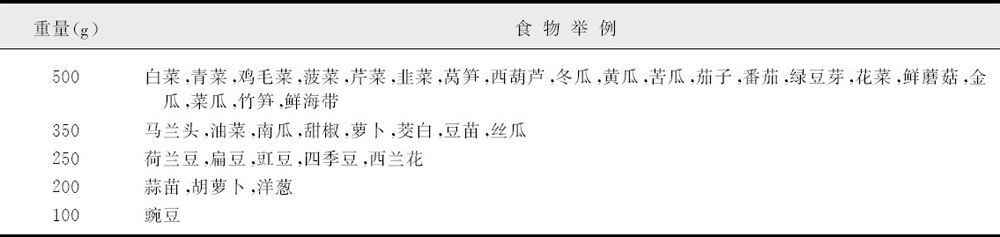
\includegraphics[width=5.91667in,height=2.82292in]{./images/Image00034.jpg}
\end{table}

\paragraph{二、职业性哮喘}

职业性哮喘近年有逐渐增多的趋势。哮喘发作与职业有关者统称职业性哮喘,诊断上应注意发病与职业上有害物质的关系。发病机制主要有:①职业接触物作为变应原,引起主要以IgE介导的速发型超敏反应;②职业有害物质引起药理介质的释放失调;③职业有害物质的非特异刺激反应,其中超敏反应起主导作用。

职业性哮喘的临床特点是:①患者在就业前不存在哮喘;②就业以后发生哮喘(一般可有数月乃至数年的潜伏期);③患病后每从事有害作业时则引起哮喘发作,脱离工作环境或假期休息时则可自行缓解,但再接触后又可发作。

工作环境中的职业性致喘物有400多种,广泛分布于化工、染料、合成纤维、橡胶皮革、纺织、制药、油漆、塑料黏合剂、印刷、冶炼、农药、木材加工、粮食、家禽饲养、农作物种植等。诊断可根据职业史和上述哮喘的特点综合考虑,必要时可行职业变应原支气管激发试验。

\paragraph{三、花粉症}

对花粉过敏者吸入花粉有的可引起气喘。花粉症在我国分布颇广,多由于黄花蒿、臭蒿、艾蒿、茵陈蒿等蒿属植物花粉所引起。此病与支气管哮喘的主要不同点是:①此病发作于花粉散发季节,且多在清晨、晴朗有风之时;②患者常伴有过敏性上呼吸道炎的表现,如流清涕、打喷嚏、鼻塞、眼和鼻奇痒,少数患者可有荨麻疹;③鼻黏膜分泌物涂片检查可发现大量嗜酸性粒细胞。以花粉作鼻黏膜激发试验,阳性率较高,有诊断意义。但应注意有的患者合并有支气管哮喘。

\paragraph{四、变应性支气管肺曲霉病(allergic bronchopulmonary}
aspergillosis,ABPA)

多由烟曲霉引起的气道高反应性疾病。对曲霉过敏者吸入大量孢子后,阻塞小支气管,引起短暂的肺不张和喘息发作,亦可引起肺部反复游走性浸润。患者表现为呼吸困难、喘息、畏寒、发热、乏力、刺激性咳嗽、咳棕黄色脓痰,偶带血。痰中有大量嗜酸性粒细胞及曲霉丝,烟曲霉培养阳性。哮喘样发作为其突出的临床表现,一般解痉平喘药难以奏效,外周血嗜酸性粒细胞增多。典型X线胸片为上叶短暂性实变或不张,可发生于双侧。胸部HRCT呈“近端”或中央支气管囊状扩张及壁增厚征象。诊断标准见第3.1.7节。

\subsubsection{7.2.3 间质性肺疾病}

间质性肺疾病(ILD)是一组主要累及肺间质、肺泡及(或)细支气管的肺部弥漫性疾病,目前已包括200多个病种,按病因明确与否分为病因已明和病因未明两大类,各病种的发病机制有显著区别,但临床上均表现为渐进性劳力性呼吸困难,限制性通气功能障碍伴弥散功能降低,低氧血症。胸部影像学显示双肺弥漫性病变,晚期发展为弥漫性肺纤维化和蜂窝肺,导致呼吸衰竭。

\paragraph{一、尘 肺}

尘肺是在生产活动中长期吸入生产性粉尘所引起的肺间质纤维化疾病,常见有硅沉着病(矽肺)、煤工尘肺、石棉肺和慢性铍肺等,重症患者有呼吸困难症状,在肺功能不全后期更为明显(参见第29节)。

\subparagraph{(一)棉尘肺}

棉纺工人发生气喘发作,须考虑是否为棉尘肺。此病的特点是,罹患此病的棉纺工人在每星期日休息之后,星期一再接触棉尘时便出现胸闷、气急、咳嗽、咳痰(部分病例可带血)等症状,但无发热。轻者工作一二天后症状渐缓解,严重者可持续至脱离接触后仍有症状。此病与长期吸入较高浓度的棉尘(尤以用低级棉为原料及粗纺车间工作者较多罹患)有关,是以支气管痉挛为基本病变的过敏性疾病。此病的主要诊断根据:①有职业史及发作的特殊规律;②肺部X线征可表现为慢性支气管炎、肺气肿征,重症者可呈广泛性网织状阴影。

\subparagraph{(二)霉草尘肺}

此病乃因接触潮湿发霉的干草,吸入带有真菌及其孢子的霉草尘所引起,罹患者以农民为多。患者常在接触后2~3小时发生呛咳、胸闷,继而咳出白色泡沫状或黏液性痰,气喘,并常有乏力、畏寒、发热等全身症状,有时出现荨麻疹。听诊双肺有弥漫性哮鸣音。血中嗜酸性粒细胞增多。X线检查可发现肺部短暂性、炎症性片状阴影及支气管周围炎征象。

所谓甘蔗渣肺也是同类疾病,见于接触发霉甘蔗渣的人。

\subparagraph{(三)蘑菇肺}

本病为蘑菇培植者的过敏性肺泡炎,也可见于平菇培植者。本病开始时易被误诊为感冒或支气管炎,主要表现为咳嗽、咳痰、胸痛、胸闷、咽痛、低热等症状,重症者有气短或呼吸困难;可有皮疹与X线肺部阴影。痰及血中常有嗜酸性粒细胞增多。本病可区分为三种临床类型:①高热型,以高热为主要症状;②支气管炎型,以支气管炎症状为主;③轻型:临床症状轻微而X线胸片有异常。X线胸片大多呈弥漫性阴影,少数呈局限性阴影。

\paragraph{二、外源性过敏性肺泡炎}

多数为在工作场所吸入了植物性或动物性有机粉尘所引起,包括农民肺、棉尘肺、霉草尘肺、甘蔗渣肺、蘑菇肺、饲鸽者肺、湿化器和空调器肺、烟草工人肺、木工肺等数十种,发病机制目前尚未完全明确,但抗原-抗体复合物和T细胞介导的免疫反应是主要的发病机制,尤其后者更为重要。

临床特点:①患者发作的症状严重程度与机体对吸入抗原的免疫反应、粉尘的抗原性、接触强度、次数及持续时间有关,可为急性、亚急性或慢性发作。②急性发作者一般在吸入大量抗原4~8小时后发作,表现为呼吸困难、干咳、胸闷,可有畏寒寒战、高热、全身不适等症状,脱离粉尘接触后1~3天内症状自然消失,少数可持续1周左右;亚急性常由急性发展而来,症状可持续数日或数周;慢性者起病隐匿,咳嗽、呼吸困难等进行性加重,常因不能及时诊治或脱离有机粉尘环境而发展为慢性肺间质纤维化,导致慢性肺心病。③用特异性抗原溶液行吸入激发试验或抗原皮肤试验常阳性。

部分急性外源性过敏性肺泡炎患者在吸入抗原后可出现哮喘症状,应与支气管哮喘鉴别,参考表\ref{tab3-4}。

\begin{table}[htbp]
\centering
\caption{外源性过敏性肺泡炎与支气管哮喘的鉴别}
\label{tab3-4}
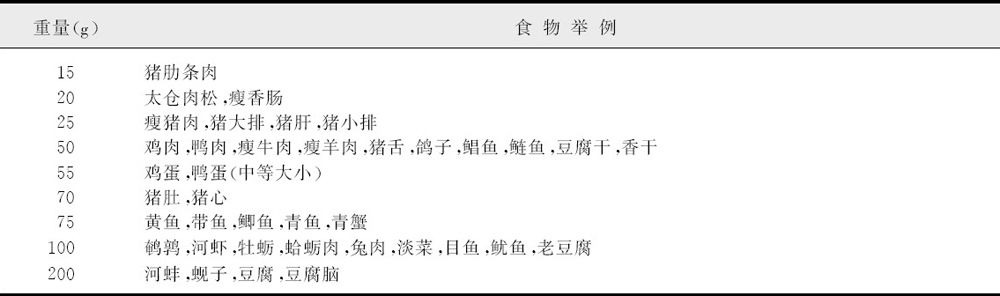
\includegraphics[width=5.90625in,height=4.09375in]{./images/Image00035.jpg}
\end{table}

\paragraph{三、特发性间质性肺炎}

特发性间质性肺炎(IIPs)是一组原因不明的肺间质性疾病,其分类与命名几经修改,目前的分类同时强调了临床-放射-病理诊断,包括了特发性肺纤维化(IPF)、非特异性间质性肺炎(NSIP)、隐源性机化性肺炎(COP)、急性间质性肺炎(AIP)、呼吸性细支气管炎间质性肺疾病(RBILD)、脱屑性间质性肺炎(DIP)、淋巴细胞性间质性肺炎(LIP)、特发性胸膜肺实质纤维弹性组织增生症(IPPF)和未分类特发性间质性肺炎(UCIIP)各自不同的实体疾病。这组疾病的临床表现非常相似,缺乏诊断特异性,但预后和治疗反应的差异性很大,故需要结合临床、放射学、肺生理功能、支气管肺泡灌洗和组织病理学等综合评估,才能明确最后诊断,并注意排除结缔组织疾病、药物、职业、感染等所致的继发性间质性肺疾病。

\subparagraph{(一)特发性肺纤维化}

特发性肺纤维化(IPF)是指原因不明并以普通型间质性肺炎(UIP)为特征性病理改变的一种慢性炎症性间质性肺疾病,占所有IIPs的60\%以上,主要表现为弥漫性肺泡炎、肺泡单位结构紊乱和肺纤维化。临床表现:①发病年龄多在中年以上,男∶女≈2∶1,儿童罕见;②起病隐袭,主要表现为干咳、进行性呼吸困难,活动后明显;③本病少有肺外器官受累,但可出现全身症状,如疲倦、关节痛及体重下降等,发热少见;④50\%左右的患者出现杵状指(趾),多数患者双肺下部可闻及Velcro啰音;⑤晚期出现发绀,偶可发生肺动脉高压、肺心病和右心功能不全等。胸片显示双肺弥漫的网格状或网格小结节状浸润影,以双下肺和外周(胸膜下)明显。HRCT是IPF诊断流程中的重要组成部分。HRCT上UIP的特征为胸膜下和肺基底部的网格状阴影和蜂窝影,常伴有牵张性支气管扩张,尤其是蜂窝影对IPF的诊断有很重要的意义。肺功能表现为限制性通气功能障碍和弥散量减少。UIP的组织病理学特征和主要诊断标准是在低倍镜下病变的不均一性,即瘢痕形成和蜂窝样改变的纤维化区域与病变轻微或正常的肺实质区域交替出现。通过有丰富ILD诊断经验的呼吸内科医生、影像科医生和病理科医生之间的多学科讨论,仔细排除其他可能的病因,是获得准确诊断最为重要的环节。诊断IPF需要符合:①排除其他已知病因的ILD(例如家庭和职业环境暴露、结缔组织疾病和药物);②未行外科肺活检的患者,HRCT呈现UIP表现;③接受外科肺活检的患者,HRCT和肺活检组织病理类型符合特定的组合。

IPF的诊断标准分为有外科(开胸/胸腔镜)肺活检资料和无外科肺活检资料。有外科肺活检资料:①肺组织病理学表现为UIP特点;②除外其他已知病因所致的间质性肺疾病,如药物、环境因素和风湿性疾病等所致的肺纤维化;③肺功能异常,表现为限制性通气功能障碍及(或)气体交换障碍;④胸片和高分辨CT(HRCT)可见典型的异常影像。无外科肺活检资料(临床诊断):缺乏肺活检资料原则上不能确诊IPF,但如患者免疫功能正常,且符合以下所有的主要诊断条件和至少3/4的次要诊断条件,可临床诊断IPF。

\hypertarget{text00046.htmlux5cux23CHP3-4-5-3-3-1-1}{}
1.主要诊断条件

①除外已知原因的ILD,如某些药物毒性作用、职业环境接触史和风湿性疾病等;②肺功能表现异常,包括限制性通气功能障碍(VC减少,而FEV\textsubscript{1}
/FVC正常或增加)及(或)气体交换障碍[静态/运动时P\textsubscript{(A-a)}
O\textsubscript{2}
增加或DLCO降低];③胸部HRCT表现为双肺网状改变,晚期出现蜂窝肺,可伴有极少量磨玻璃影;④经支气管肺活检(TBLB)或支气管肺泡灌洗液(BALF)检查不支持其他疾病的诊断。

\hypertarget{text00046.htmlux5cux23CHP3-4-5-3-3-1-2}{}
2.次要诊断条件

①年龄>50岁;②隐匿起病或无明确原因进行性呼吸困难;③病程≥3个月;④双肺听诊可闻及吸气性Velcro音。

2011年ATS/ERS/JRS/ALAT更新了关于IPF诊治的询证医学指南,其诊断标准如下:

1.排除其他已知原因的间质性肺疾病(如家庭或职业环境暴露、结缔组织疾病和药物毒性)。

2.未施行外科肺活检的患者HRCT表现为典型UIP型。

3.施行外科肺活检的患者应结合HRCT和外科肺活检病理类型[尤其是HRCT或(和)组织病理学不典型时]。

典型UIP型HRCT诊断标准(所有4个特征):病灶以胸膜下、基底部为主;网格状异常改变;蜂窝肺伴或不伴牵张性支气管扩张;无不符合UIP型所列的CT特征。

UIP型的组织病理学标准(所有4条标准):以胸膜下或间隔旁分布为主的明显纤维化和结构紊乱的证据,伴或不伴蜂窝;肺实质斑片状纤维化改变;出现成纤维细胞灶;无不支持UIP诊断的病理特征。

\subparagraph{(二)非特异性间质性肺炎}

非特异性间质性肺炎(NSIP)为IIPs的一种,病因不清,国内一组8例报道中3例可能与环境暴露(棉尘、沙尘、动物皮毛、挥发性酸性化合物)有关。国外报道多以风湿性疾病为病因。其临床表现和影像学与IPF类似,主要表现为咳嗽、呼吸困难、双下肺可闻及Velcro啰音;胸片表现为中下肺野为主的网状阴影,有时表现为斑片阴影;HRCT显示双肺对称性磨玻璃影或双肺肺泡腔的实变影。

NSIP与IPF临床上的主要鉴别有:①IPF发病年龄(平均57岁)大于NSIP(平均49岁)。②IPF多见于男性;NSIP多见于女性。③IPF起病多隐匿,就诊时通常已有1~2年病史;NSIP起病多呈亚急性,从出现症状到确诊很少超过1年。④IPF患者发热很少见,杵状指多见;NSIP可有发热(22\%~33\%),杵状指少见。⑤IPF对糖皮质激素治疗不敏感;NSIP对激素反应良好。⑥IPF预后差,死亡率60\%~90\%;NSIP预后良好,死亡率0\%~29\%。

\paragraph{四、结节病}

结节病是一种多系统器官受累的肉芽肿性疾病,常侵犯肺、双侧肺门淋巴结,也可侵犯其他器官,病因尚未十分明确,可能与遗传因素、特殊病原体的感染(病毒、支原体、真菌等)、自身免疫、吸入无机物(铝、锆、滑石)或有机物(枫树粉、黏土)等有关。早期呼吸道症状较轻,多为干咳,无痰或少痰,后期可因肺纤维化导致呼吸困难。(参见第26.1节)。

\paragraph{五、肺嗜酸性粒细胞浸润症}

肺嗜酸性粒细胞浸润症是一组由嗜酸细胞浸润引起的肺部病变,常伴有外周血嗜酸性粒细胞增多。病因与发病机制尚不完全清楚,可能与变态反应或免疫反应异常有关。临床上主要表现有不同程度的胸闷、咳嗽、喘息、呼吸困难、乏力、低热等症状。

\subparagraph{(一)单纯性肺嗜酸性粒细胞浸润症}

又称吕弗勒综合征,其病因与发病机制尚不完全清楚,可能与寄生虫感染(蛔虫、钩虫、丝虫、绦虫、姜片虫、阿米巴原虫等)和某些药物(对氨基水杨酸、阿司匹林、磺胺制剂等)引起的肺部Ⅰ型和Ⅲ型变态反应有关,其他病因可能为吸入花粉、真菌孢子等。

本病国内报道颇多,其临床表现一般较轻,患者有全身不适、乏力、低热、干咳等症状,大多咳少量的黏稠痰液。少数患者症状较重,表现为高热、哮喘或呼吸困难。体检胸部体征轻微,可有少量干湿音或全无体征,与肺部X线摄片所见不相称。血象白细胞总数正常或稍增高,分类计数嗜酸性粒细胞明显增加,多数在10\%~20\%,偶达70\%~80\%,绝对计数达(1.0~2.5)×10\textsuperscript{9}
/L。血象改变通常在发病10~15天后消失。肺部X线征极不一致,可呈片状、圆形、粟粒样、结节状、条状或不规则的阴影,病灶附近肺纹理增加;有时肺部X线征呈游走性变化,此起彼伏,并多于发病6~12天后消失,很少延长至一个月以上。

诊断本病的主要依据是:①病程短促与良性经过;②上述的症状与体征;③外周血嗜酸性粒细胞增多;④X线检查肺部有短暂性浸润阴影,消散后不留痕迹。

在鉴别诊断上本病须与肺结核、肺炎支原体肺炎、不完全性大叶性肺炎、热带肺嗜酸性粒细胞增多症等相区别。因X线摄片上可能出现大片阴影,类似浸润性肺结核或干酪样肺炎,或呈粟粒样阴影而类似粟粒型肺结核,或偶尔肺部浸润消散过程中出现假性空洞而类似肺结核空洞形成。根据肺结核的全身中毒症状较重,X线复查肺部阴影不可能在短期内消散,血象中无嗜酸性粒细胞增多,痰中可查到抗酸杆菌等现象,一般鉴别不难。肺炎支原体肺炎的肺部阴影虽可于较短期内消散,但无嗜酸性粒细胞增多,且常有较高效价的冷凝集反应。大叶性肺炎不仅无嗜酸性粒细胞增多,而且症状较重和体征明显,据此可与本综合征相区别。

本综合征与热带肺嗜酸性粒细胞增多症的鉴别诊断参考表\ref{tab5-5}。

\subparagraph{(二)热带嗜酸性粒细胞浸润症}

本病病情严重时可有哮喘样发作,也可以哮喘样发作突然起病(参见第16节)。

\subparagraph{(三)慢性嗜酸性粒细胞性肺炎}

慢性嗜酸性粒细胞性肺炎(CEP)病因与发病机制不清楚,可能与自身免疫有关。本病病程较单纯性肺嗜酸性粒细胞增多症长,通常为2~6个月,甚至一年以上。多见于中青年女性,临床上起病缓慢,常见发热、干咳或咳少量黏稠样痰、盗汗、体重减轻;约1/3患者合并哮喘,可有喘息、进行性呼吸困难以及呼吸衰竭。外周血嗜酸性粒细胞多增高,比例可达20\%~70\%。胸部X线显示非段或叶性分布的片状阴影,常为外侧外带分布,出现特征性的“肺水肿反转征”,阴影可有一定的游走性,予糖皮质激素治疗后阴影迅速消失。

\paragraph{六、嗜酸性肉芽肿性多血管炎}

原称为变应性肉芽肿性血管炎,又称Churg-Strauss综合征(CSS),是一种以多器官系统发生肉芽肿性血管炎为特征的少见疾病,肺部血管最易受累。病因与发病机制均不清楚,主要临床表现为支气管哮喘、过敏性鼻炎、外周血嗜酸性粒细胞增多和多器官组织坏死性血管炎,周围形成肉芽肿及大量嗜酸性粒细胞浸润为特征。

1990年美国风湿病协会提出本病的6项诊断标准为:①哮喘;②外周血嗜酸性粒细胞增多,分类计数>10\%;③单发性或多发性神经病变;④游走性或一过性肺浸润;⑤鼻窦病变;⑥组织活检证实有血管外嗜酸性粒细胞浸润。凡患者有上述6项标准中4项或以上者可诊断本病,诊断敏感性85.0\%,特异性99.7\%。

本病主要须与Wegener肉芽肿相鉴别:本病主要表现为支气管哮喘,过敏性鼻炎,鼻腔病变多为弥漫性鼻黏膜肿胀、鼻息肉,累及肾脏时病变程度较轻;而Wegener肉芽肿鼻腔病变多为鼻溃疡、凝固性或液化坏死性肉芽肿,肺内浸润易形成空洞,且肾损害较严重,而没有支气管哮喘和外周血嗜酸性粒细胞增高。

\paragraph{七、淋巴细胞间质性肺炎}

淋巴细胞间质性肺炎以渐进性活动后气促、咳嗽、消瘦为主征,严重者呼吸困难与发绀。体检双下肺可闻小水泡音及爆裂音。X线胸片示双侧中、下肺野以中内带为主的广泛网状阴影,夹杂以小结节阴影。经纤支镜下肺组织病理活检可确诊。泼尼松治疗疗效好。

淋巴细胞性间质性肺炎(LIP)是临床少见疾病,2002年美国胸科协会(ATS)及欧洲呼吸协会(ERS)发布的国际多学科共识意见将特发性间质性肺炎分为七类,LIP为其中之一。LIP起病隐匿,病程长,多数患者为女性,男女的比例约为1∶2,发病年龄从40~70岁不等,诊断时的平均年龄在52~56岁。呼吸系统的主要症状是干咳、逐渐加重的呼吸困难,偶有发热、盗汗、体重下降。胸部查体可发现双肺底爆裂音,杵状指(趾)少见。外周及纵隔淋巴结肿大及脾大很少见。肺功能通常提示限制性通气功能障碍及(或)弥散功能减低。高分辨CT表现为小叶中心性结节、胸膜下结节、双下肺为主的毛玻璃样斑点影、支气管血管束增厚。LIP的诊断实质上是病理诊断,LIP的病理特点是多克隆的成熟的小淋巴细胞弥漫浸润肺间质,包括小叶间隔、肺泡间隔,细胞成分以淋巴细胞为主,伴有浆细胞、组织细胞、上皮细胞等。

\paragraph{八、原发性呼吸道淀粉样变性}

淀粉样变性是一组表现各异的临床综合征,共同点是组织或器官的细胞外淀粉样蛋白质沉积,可累及全身器官,但如仅累及呼吸道时,则称原发性呼吸道淀粉样变性。本病少见,起病隐袭缓慢,主要表现为咳嗽、咳痰、进行性呼吸困难,可有咯血。纤支镜下活检可作出诊断。

国内曾报道三例患者,均为男性,纤支镜检查显示不同程度气管及(或)支气管不规则狭窄,不同叶、段支气管管腔狭窄至闭塞,管腔内有小结节状突起,黏膜水肿,充血,有出血或出血倾向。活检病理检查证实支气管黏膜下淀粉样变性:苏木素伊红染色黏膜内有大片絮状不规则无细胞的嗜伊红物质沉积,刚果红染色呈玫瑰红色,有双折光性,在偏光显微镜下刚果红阳性处呈绿色。

\paragraph{九、肺泡蛋白质沉积症}

本病可引起进行性气促,严重者可呈明显呼吸困难和发绀。乃由于肺泡及细支气管内充满PAS染色阳性的颗粒状类蛋白质物质所致(参见第15节)。

\subsubsection{7.2.4 阻塞性病变}

\paragraph{一、慢性阻塞性肺疾病}

慢性阻塞性肺疾病(COPD)是一种具有气流受限特征的肺部疾病,气流受限不完全可逆,呈进行性发展。确切的病因还不十分清楚,但认为与肺部对有害气体或有害颗粒的异常炎症反应有关。支气管哮喘(其为一种特殊的气道炎症性疾病,其气流受限具有可逆性)和一些已知病因或具有特征病理表现的气流受限疾病(如肺囊性纤维化、弥漫性泛细支气管炎、闭塞性细支气管炎等)不属于COPD的范畴。

COPD的起病缓慢,病程较长,主要症状为慢性咳嗽、咳痰,一般为白色黏液或浆液性泡沫性痰;气短或呼吸困难,早期在劳力时出现,以后呈进行性加重,是COPD的标志性症状;部分患者特别是重度患者或急性加重时出现喘息、胸闷;晚期患者有体重下降,食欲减退等。早期体征可无异常,随疾病进展可出现典型肺气肿体征:桶状胸,肺部叩诊过清音,心浊音界缩小,肺下界和肝浊音界下降,双肺呼吸音减弱,呼气延长,部分患者可闻及干啰音及(或)湿啰音。

COPD的诊断可根据吸烟等高危因素史、临床症状、体征及肺功能检查等综合分析确定。诊断的必备条件是肺功能检查显示不完全可逆的气流受限,即吸入支气管舒张药后FEV\textsubscript{1}
/ FVC<70\%及FEV\textsubscript{1}
<80\%预计值。无肺功能检查仪时可行用力呼气时间听诊法进行估计:被检者深吸气后屏气,然后用力尽快将气呼出。检查者将听诊器置于患者气管或胸骨上段,计算用力呼气时间,从呼气开始至呼气终止这段时间为最大呼气时间。正常不超过4秒,轻度阻塞者通常在6秒以内,中、重度阻塞者在6秒以上。

\paragraph{二、阻塞性肺不张}

急性大片阻塞性肺不张起病急骤,常有呼吸困难、心动过速,有时伴有休克现象;缓慢发展的肺不张,患者可无自觉症状。

阻塞性肺不张由于支气管内黏膜高度水肿、分泌物、瘢痕收缩、异物、支气管恶性或良性肿瘤、结核病变等阻塞支气管腔所引起。

大片阻塞性肺不张的主要体征是患侧胸廓凹陷,肋间变窄,呼吸运动减弱,膈肌升高,气管、心脏与纵隔向患侧移位。患侧部位叩诊可呈浊音,呼吸音减弱或消失;但也有叩诊无浊音者,其原因是由于邻近肺组织产生代偿性肺气肿。诊断主要根据临床表现与X线检查。

急性阻塞性肺不张往往伴有感染,引起发热、咳嗽,须与大叶性肺炎相区别。后者常由肺炎链球菌感染所致,有寒战、高热、胸痛,咳嗽较显著,可咳出铁锈色痰,无气管与纵隔的移位。X线检查有助于二者的区别。

阻塞性肺不张亦需与压迫性肺不张相鉴别,后者是由于胸腔积液、气胸,肺内或胸腔内肿瘤,肺包虫病,胸廓畸形,呼吸肌或膈肌麻痹,纵隔肿瘤,淋巴结肿大,扩大的心脏,胸内甲状腺,膈疝,主动脉瘤及腹腔巨大肿瘤、大量腹水使膈肌升高等所引起。其体征与阻塞性肺不张不同,因不同病因而异。

\paragraph{三、弥漫性泛细支气管炎}

弥漫性泛细支气管炎是一种原因不明的、以弥漫存在于两肺细支气管和呼吸性细支气管区域并累及管壁全层的慢性炎症为特征的疾病。1969年首先由日本学者山中、本间、谷木等提出,可表现为慢性咳嗽、多痰和劳力性呼吸困难,并伴有气流受限。慢性的咳嗽和较多的脓痰等症状的进展多见于20~50岁人群,随后逐渐出现劳力性呼吸困难。肺部听诊可闻及爆裂音、哮鸣音。胸部CT表现为弥漫性小结节影和线状阴影,小叶中心性小颗粒状,与胸壁有少许间隔为其特点;小支气管和细支气管扩张,以两肺下叶最明显;支气管壁增厚;易合并中叶和舌叶肺不张。

1998年日本厚生省临床诊断标准:

\subparagraph{1.必要条件}

①持续咳嗽、咳痰及活动时呼吸困难;②合并有慢性鼻窦炎或有既往史;③胸部X线见两肺弥漫性散在分布的颗粒样结节状阴影或胸部CT见两肺弥漫性小叶中心性颗粒样结节状阴影。

\subparagraph{2.参考条件}

①胸部间断性湿啰音;②第1秒用力呼气容积与用力肺活量比值(FEV\textsubscript{1}
/ FVC\%)<70\%,动脉血氧分压(PaO\textsubscript{2}
)<80mmHg;③血清冷凝集试验效价>1∶64。

\subparagraph{3.临床诊断}

(1)临床确诊:必要条件①+②+③加参考条件中>2项。

(2)临床高度可疑诊断:必要条件①+②+③。

(3)临床可疑诊断:必要条件①+②。

临床上要与慢性阻塞性肺疾病、支气管扩张、支气管哮喘等疾病鉴别。

\subsubsection{7.2.5 其他原因}

\paragraph{一、急性肺损伤与急性呼吸窘迫综合征}

急性肺损伤(ALI)/急性呼吸窘迫综合征(ARDS)是指由心源性以外的各种肺内外致病因素导致的急性、进行性缺氧性呼吸衰竭。ALI和ARDS具有性质相同的病理生理改变,ARDS是严重的ALI。其主要病理基础是由多种炎症细胞(巨噬细胞、中性粒细胞和淋巴细胞等)介导的肺脏局部炎症反应和炎症反应失控所致的肺毛细血管膜损伤。主要病理特征为由于肺微血管通透性增高而导致的肺泡渗出液中富含蛋白质的肺水肿及透明膜形成,可伴有肺间质纤维化。病理生理改变以肺顺应性降低,肺内分流增加及通气血流比例失调为主。2012年由欧洲危重病医学会(ESICM)与美国胸科学会(ATS)组成的联合委员会于2012年发表了ARDS柏林定义。根据柏林定义,ARDS是一种急性弥漫性肺部炎性反应,可导致肺血管通透性升高,肺重量增加,参与通气的肺组织减少。

临床表现为呼吸频数和呼吸窘迫、顽固性低氧血症,而动脉血二氧化碳分压(PaCO\textsubscript{2}
)正常,早期肺部听诊无明显异常,病情进展肺部可听到干、湿啰音。胸部X线显示双肺弥漫性浸润影,后期常并发多器官功能衰竭。

ARDS的高危因素包括直接肺损伤因素(严重肺感染、胃内容物吸入、肺挫伤、吸入有毒气体、淹溺、氧中毒等)和间接肺损伤因素(脓毒症、严重的非胸部创伤、重症胰腺炎、大量输血、体外循环、DIC等)。

1994年欧美共识会议(AECC)发表ARDS诊断标准:①急性起病;②氧合指数(PaO\textsubscript{2}
/ FiO\textsubscript{2}
)≤200mmHg(1mmHg=0.133kPa,不考虑PEEP因素);③正位胸片显示双肺斑片状浸润影;④肺动脉楔压(PAWP)≤18mmHg,或无左心房压力增高的临床证据。2000年中华医学会呼吸病学分会起草提出了ALI/ARDS的诊断标准(草案)与AEEC标准基本相同。

近年来临床研究显示,欧美共识会议诊断标准的敏感性为84\%,而特异性仅为51\%。2011年欧洲重症医学会柏林会议在ARDS流行病学、病理生理学和临床研究基础上,提出了ARDS柏林新定义。该定义将ARDS患者分为轻、中、重3个层次,其中轻度取代了ALI,建议废除ALI的命名。其临床诊断的有效性和准确性尚有待进一步证实(表\ref{tab3-5}\footnote{a:胸片或CT;b:如海拔>1000m,按以下公式纠正:[PaO\textsubscript{2}
/FiO2×(大气压/760)];c:轻度ARDS可用无创通气})。

\begin{table}[htbp]
\centering
\caption{急性呼吸窘迫综合征的柏林定义}
\label{tab3-5}
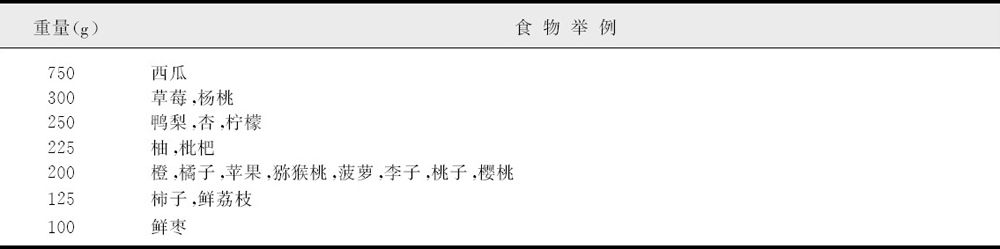
\includegraphics[width=5.89583in,height=2.01042in]{./images/Image00036.jpg}
\end{table}

ARDS诊断时须排除大片肺不张、自发性气胸、上气道阻塞、急性肺栓塞和心源性肺水肿等。与心源性肺水肿的鉴别可根据下列几点:

1.心源性肺水肿的呼吸困难与体位有关,而ARDS则不太明显。

2.心源性肺水肿咳粉红色泡沫样痰,而ARDS的血痰多非泡沫性,而为稀血水样。

3.心源性肺水肿对强心苷、利尿药和血管扩张药有较佳的治疗反应,而ARDS即使吸入高浓度氧疗效不显著。

4.心源性肺水肿湿啰音多集中于肺底,而ARDS的湿啰音分布较广泛,且音调较高,常呈“爆裂音”。

5.心源性肺水肿X线胸片异常阴影与相应的临床表现几乎同时出现,对及时的急救治疗反应常迅速;而ARDS的X线胸片所见疑似肺泡性水肿,但经积极抢救X线征象在数日内无明显好转。鉴别困难时,可通过超声心动图检测心室功能等作出判断并指导此后的治疗。

\paragraph{二、肝肺综合征}

肝肺综合征(HPS)是指肝功能不全引起肺血管扩张、肺气体交换障碍导致的低氧血症及其一系列的病理生理变化和临床表现。常把肝功能不全、肺血管扩张和低氧血症三联症称为HPS。HPS常见于肝炎后肝硬化、酒精性肝硬化及其他原因肝硬化,也可见于慢性活动性肝炎、急性暴发性肝炎、胆汁淤积、非肝硬化性门脉高压(如门体静脉或脾肾静脉吻合手术后)等。国内曾报道两组分别为6例和16例的HPS,均在乙型肝炎、丙型肝炎、酒精性肝病、Wilson病所致的肝硬化基础上发生。

HPS临床上除了肝病的一般表现外,还存在与肝病有关的低氧血症,表现为活动性呼吸困难、发绀、杵状指,其原理是由于肺血管扩张引起的通气/灌注和弥散功能失调。目前认为肺内血管扩张的发生与肺血管扩张物质(如血管活性肠肽等)在肝功能不全时不能被灭活,或经门体分流和淋巴通道进入肺循环,也可能是内皮素、血管紧张素Ⅰ等缩血管物质的缺乏或被抑制,或肺血管内皮细胞对缩血管物质敏感性的下降,致使原关闭的无功能性毛细血管前交通支开放,以及原本正常的低氧性肺血管收缩功能发生障碍。HPS的缺氧表现为直立位低氧,即由卧位改变为直立位时呼吸困难和发绀加剧,PaO\textsubscript{2}
下降10mmHg以上,这是因为肺血管扩张主要位于两肺基底部,直立位时因重力作用影响,流经肺下野的血流量增多,致使肺内右至左分流量增多,氧合障碍进一步加重,缺氧加剧。

确定肺血管扩张是诊断HPS的关键,符合下列条件的可以诊断为HPS:①急、慢性肝脏疾病;②没有原发性心肺疾病,胸片正常或有间质结节状阴影;③肺气体交换异常,有或无低氧血症,P\textsubscript{(A-a}
)O\textsubscript{2}
梯度>15mmHg;④对比增强超声心动描记术(CTTE)及(和)肺灌注扫描,肺血管造影存在肺血管扩张及(或)肺内血管短路;⑤直立位缺氧、气短、发绀,肺骨关节病。诊断标准:肝硬化基础上+微发泡试验阳性+直立位低氧血症(PaO\textsubscript{2}
<70mmHg,即可诊断HPS。如肝硬化基础上+微发泡试验阳性+无直立位低氧血症,说明有肺血管扩张,尚未达到HPS。

\protect\hypertarget{text00047.html}{}{}

\subsection{7.3 胸膜疾病}

\subsubsection{一、自发性气胸}

自发性气胸多以骤然发生的患侧胸痛与呼吸困难起病。严重者(多为张力性气胸)呈进行性呼吸困难、发绀,甚至出现休克。体检发现患侧胸廓饱满,呼吸运动减弱,触觉语颤减弱或消失,叩诊呈鼓音,听诊肺泡呼吸音减弱或消失。气管、心脏与纵隔向健侧移位。临床上一经诊断为张力性自发性气胸,不必等待X线诊断,应立即进行胸腔穿刺排气。

自发性气胸可分成原发性和继发性。继发性发生在有基础肺疾病的患者,由于病变引起细支气管不完全阻塞,形成肺大疱破裂,如肺结核、COPD、肺癌、肺脓肿、尘肺等;原发性发生在无基础肺疾病的健康人,多见于瘦高体型的男性青壮年,常规X线检查肺部无显著病变,但胸膜下可有肺微小疱,多在肺尖部。

根据脏层胸膜破裂情况不同及其发生后对胸腔内压力的影响,自发性气胸通常分为三种临床类型:闭合性(单纯性)、交通性(开放性)及张力性(高压性),见表\ref{tab3-6}。

\begin{table}[htbp]
\centering
\caption{各类型自发性气胸的鉴别}
\label{tab3-6}
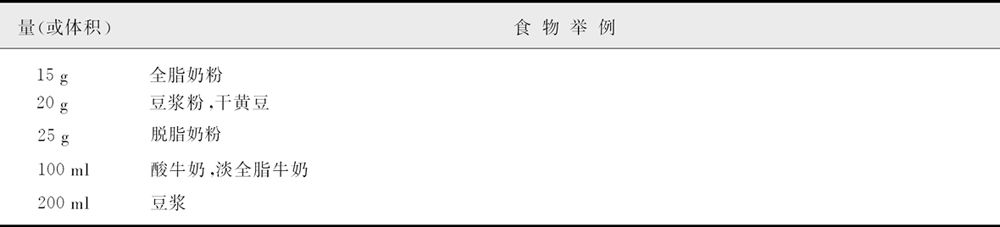
\includegraphics[width=5.91667in,height=2.65625in]{./images/Image00037.jpg}
\end{table}

继发性自发性气胸中最常由肺结核引起,肺结核病灶破裂的特点是:①患者常有发热等结核感染中毒症状;②如有胸腔积液,常为脓性,量常较多;③肺部X线检查通常无肺气肿或肺大疱。

自发性气胸须与肺大疱相区别,主要根据:①后者症状不明显或较轻;②胸部X线检查肺大疱的气腔位于肺实质中,因此在肺尖和肋膈角仍可见有肺组织,并可见气腔内有纤维条索状影像走向肺门,而气胸的气体位于胸腔内,肺组织被推向肺门;③肺大疱有整齐、致密而菲薄的线状泡壁,气腔呈圆形或椭圆形。

\subsubsection{二、大量胸腔积液}

由于大量胸腔积液,压迫肺组织产生压迫性肺不张,使肺呼吸面积减少;同时使纵隔向健侧移位,以致发生呼吸困难。呼吸困难一般发生较缓慢。其严重程度取决于积液产生的速度及其量的大小。急速大量积液时,呼吸困难较明显;积液缓慢发生者,有时可因患者逐渐适应而无呼吸困难。胸腔积液的病因较繁杂(参见第33节)。

\protect\hypertarget{text00048.html}{}{}

\subsection{7.4 纵隔疾病}

\subsubsection{一、急性纵隔炎(参见第33节)。}

\subsubsection{二、慢性纤维性纵隔炎}

慢性纤维性纵隔炎多继发于化脓性或结核性纵隔炎之后,病理改变为纤维组织增生与瘢痕收缩,病变可为广泛性或局限性,症状因纵隔组织受累不同而表现不一。如压迫气管、支气管,则出现气短与呼吸困难;如压迫上腔静脉,则出现上腔静脉阻塞综合征(参见第38节);如压迫喉返神经,则出现声音嘶哑;压迫食管则引起吞咽困难。

\subsubsection{三、纵隔肿瘤及囊肿}

纵隔肿瘤及囊肿发展到一定阶段,压迫或侵犯气管或大支气管时,可引起不同程度的呼吸困难(参见第27.1节)。

\subsubsection{四、纵隔气肿}

严重的纵隔气肿可引起呼吸困难(参见第33节)。

\protect\hypertarget{text00049.html}{}{}

\subsection{7.5 胸廓运动及呼吸肌功能障碍}

胸廓运动受限、呼吸肌和膈肌麻痹、膈高位等皆可使肺呼吸面积减少,而引起呼吸困难。严重的胸廓畸形、肋软骨骨化及硬皮病等均可使胸廓活动受限制;呼吸肌及膈肌麻痹,常由于脊髓灰质炎,脊髓创伤、脑膜炎或脊柱结核所致的神经根病变,多发性神经根神经炎,白喉,重症肌无力等所引起;主动脉瘤可压迫左侧膈神经,肺门部肿瘤或转移瘤也可侵犯膈神经而使膈肌麻痹;膈肌高位常见于妊娠后期、高度的腹水、人工气腹或鼓肠、巨大的腹腔内肿瘤等。

膈肌麻痹

膈肌麻痹分为单侧膈肌麻痹和双侧膈肌麻痹,一般来说单侧膈肌麻痹远多于双侧膈肌麻痹。常见发病原因包括创伤、压力相关、炎症以及神经源性和特发性。其临床表现多种多样,从无症状至呼吸衰竭均可出现,部分患者可表现为重度劳累性呼吸困难以及平卧位呼吸困难,尤其是在夜间快速动眼期可以出现夜间低氧血症和高碳酸血症。因为膈肌麻痹的临床症状无显著特殊性,所以临床上常常误诊为冠状动脉粥样硬化性心脏病、肺炎、肺不张等疾病,据报道平均误诊时间可达2年左右。影像学检查对于诊断膈肌麻痹尤其是单侧膈肌麻痹意义重大,但是对于双侧膈肌麻痹则误诊率高。最大跨膈压检测是诊断膈肌麻痹的金指标。

\protect\hypertarget{text00050.html}{}{}

\subsection{7.6 肺血管病变}

\subsubsection{一、肺栓塞}

肺栓塞和肺梗塞二者有不同的涵义。体循环静脉中或右心的栓子,沿血流进入并堵塞肺动脉或其分支,称为肺栓塞。栓塞部分的肺组织,可因缺氧、坏死而形成肺梗塞。肺栓塞并非都引起肺梗塞。肺梗塞在病理解剖上属于出血性梗塞范畴。

肺栓塞(PE)是以各种栓子阻塞肺动脉系统为其发病原因的一组疾病或临床综合征的总称,包括肺血栓栓塞症(PTE)、脂肪栓塞综合征、羊水栓塞、空气栓塞等。我国由于既往对此病认识不足,临床上经常误诊、漏诊,近年来的研究表明,肺栓塞在我国并非少见。

肺栓塞常见的危险因素和基础病因包括深静脉血栓形成(DVT)、恶性肿瘤、各种心脏病、结缔组织病(系统性红斑狼疮、抗磷脂综合征等)、肾病综合征、外伤、手术和妊娠等。国内一组63例和一组39例的肺栓塞的报道显示最常见的临床症状为呼吸困难、咯血、心悸、胸痛、咳嗽,部分患者有发热、发绀、晕厥等。

\paragraph{(一)肺血栓栓塞症}

PTE为来自静脉系统或右心的血栓阻塞肺动脉或其分支所致的疾病,以肺循环和呼吸功能障碍为其主要临床和病理生理特征。引起PTE的血栓可以来源于下腔静脉径路、上腔静脉径路或右心腔,其中大部分来源于下肢深静脉,特别是从腘静脉上端到髂静脉段的下肢近端深静脉(约占50\%~90\%)。PTE为PE的最常见类型,占PE中的绝大多数,通常所称PE即指PTE。

PTE的临床症状多种多样,均缺乏特异性,症状的严重程度亦有很大差别,可以从无症状到血流动力学不稳定,甚或发生猝死。常见症状包括:呼吸困难及气促、胸痛、晕厥、烦躁不安、惊恐甚至濒死感、咯血、发热等。体检可见呼吸急促、脉速、低血压甚至休克,发绀、颈静脉充盈或搏动、肺部可闻及哮鸣音及(或)细湿啰音,胸腔积液时有相应体征。体检时要注意有否下肢肿胀、压痛、浅静脉扩张、皮肤色素沉着等。

如怀疑PTE,尽快行血浆D-二聚体检测,含量<500mg/L可排除诊断;超声检查可以提示PTE和排除其他疾病;放射性核素肺通气/灌注扫描具有较为重要的诊断或排除诊断意义;螺旋CT、电子束CT或MRI有助于发现肺动脉内血栓的直接证据,已成为临床上经常应用的重要检查手段;肺动脉造影是诊断的“金标准”和参比方法,但为有创性,费用较高。以上检查可根据具体情况选用。

PTE须与急性心肌梗死以及大叶性肺炎相鉴别。急性心肌梗死疼痛多位于心前区,患者有高血压或动脉粥样硬化病史,体温增高较迟于PTE,多在第二、三天才出现,如有咯血与肺局部体征,则更不支持急性心肌梗死的诊断。PTE的典型心电图呈S\textsubscript{Ⅰ}
Q\textsubscript{Ⅲ} T\textsubscript{Ⅲ}
征(即Ⅰ导联S波加深,Ⅲ导联出现Q/q波及T波倒置),往往有完全或不完全性右束支传导阻滞,肺型P波,电轴右偏及顺钟向转位等,如病情好转,心电图改变在较短期间恢复正常,与急性心肌梗死特征性的心电图改变及动态衍变不同,且急性心肌梗死有动态的心肌酶学水平改变。X线检查PTE可发现肺部阴影、肺底浸润或肋膈角模糊阴影,而急性心肌梗死如无发生心力衰竭出现肺水肿则一般没有肺部阴影。大叶性肺炎先有寒战、高热,其后才发生胸痛、咳铁锈色痰,可有唇周疱疹,有典型的胸部X线大叶实变阴影,与PTE不同。

\paragraph{(二)羊水栓塞}

羊水栓塞少见,为一种产科急症,为妊娠期羊水中胎儿产物(胎儿的上皮、毛发、胎脂、黏蛋白、胎粪)进入母体循环而引起。常表现为产妇在破水后不久,突然出现呼吸困难、发绀、抽搐,或兼有休克、昏迷等症状,临床医师应立即考虑此病的可能性,并马上进行诊断与抢救。

发病机制主要由于羊水中胎儿产物作为栓子进入母体循环后可引起肺血管栓塞、变态反应性休克、凝血机制障碍甚至并发弥散性血管内凝血(DIC),影响脏器供血和脏器功能。患者大多数为足月妊娠的中年经产妇,在伴有子宫强烈收缩的情况下发病。由于其发生极其迅速、凶险,病理生理学机制复杂,加之临床医生对它缺乏足够的认识,往往不能及时作出处理,导致母婴死亡率都很高,产妇多因休克、肺水肿或产后大出血而死亡。

肺羊水栓塞有时须与肺血栓栓塞相区别,后者发生于产后静脉血栓形成的基础上,多于产后一周间出现。

\subsubsection{二、肺动脉高压}

肺动脉高压是指孤立的肺动脉血压增高,而肺静脉压力正常,主要原因是肺小动脉原发病变或其他的原发疾病而导致的肺动脉阻力增加,表现为肺动脉压力升高而肺静脉压力在正常范围内,需要肺毛细血管楔压正常才能诊断。肺动脉高压临床表现无特异性,最常见的首发症状是活动后气短、乏力,其他症状有胸痛、咯血、眩晕或晕厥、干咳。气短往往标志肺动脉高压患者出现右心功能不全。而当发生晕厥或眩晕时,则往往标志患者心输出量已经明显下降。查体可见P2亢进;肺动脉瓣开放突然受阻出现收缩早期喷射性喀喇音;三尖瓣关闭不全引起三尖瓣区的收缩期反流杂音;晚期右心功能不全时出现颈静脉充盈或怒张;下肢水肿;发绀;右室充盈压升高可出现颈静脉巨大α波;右室肥厚可导致剑突下出现抬举性搏动;出现S3表示右心室舒张充盈压增高及右心功能不全,约38\%的患者可闻及右室S4奔马律。超声心动图是筛查肺动脉高压最重要的无创性检查方法,可用于估测肺动脉收缩压、评估病情严重程度及预后并协助明确病因。而右心导管检查是确诊肺动脉高压的金标准。

\subsubsection{三、肺静脉堵塞病}

肺静脉堵塞病(pulmonary veno-occlusive
disease,PVOD)是导致肺动脉高压少见的原因之一,它是一种因肺小静脉弥漫性阻塞导致的严重肺动脉高压病,病因目前仍不明确,该病与特发性肺动脉高压临床表现相似,易误诊。目前报道例数较少,对该病的认识不多。床上应用靶向药物治疗反应不佳的肺动脉高压,很可能是被误诊的PVOD,约占最初诊断为特发性肺动脉高压的5\%~10\%。其主要表现为活动后进行性呼吸困难,还有其他症状,如咳嗽、咯血、胸痛、乏力、嗜睡及晕厥等,少数患者可出现弥漫性肺泡内出血和猝死。晚期可出现右心功能不全和右心衰竭的症状和体征,如呼吸频数、发绀、颈静脉怒张、肝颈静脉回流征阳性,心脏听诊P2亢进和三尖瓣反流性杂音,伴有肺部浸润的患者双肺可闻及湿性啰音。此外,PVOD容易合并胸腔积液、心包积液,很少一部分患者也可出现杵状指。胸部影像学特点主要为肺水肿的征象,胸部平片和高分辨率螺旋CT可发现肺充血,Kerley
B线或胸腔积液,肺动脉高压,右心房、右心室扩大,左心房正常等征象。2009年欧洲心脏协会和呼吸协会共同制定该病指南,制定临床诊断标准主要依据:①严重肺动脉高压症状及体征;②胸部影像学提示肺水肿、Kerley
B线或胸腔积液,高分辨CT发现小叶中央毛玻璃样模糊影、间隔线、纵隔淋巴结肿大;③肺动脉楔压(pulmonary
artery wedge
pressure,PAWP)正常或左心房内径正常。符合上述标准可临床诊断为PVOD,不一定需要病理学证据。

\protect\hypertarget{text00051.html}{}{}

\section{8 心源性呼吸困难}

呼吸困难是心功能不全的重要症状之一,其产生的主要原因是:①长期肺淤血,导致肺泡弹性减退,通气功能障碍;②心排血量减少与血流速度减慢,换气功能障碍,导致缺氧与二氧化碳潴留;③肺循环压力增高,导致反射性呼吸中枢兴奋性增高。

心源性呼吸困难的临床特点可概括如下:①患者有重症心脏病存在;②呈混合性呼吸困难,坐位或立位减轻,卧位时加重;③肺底部出现中、小湿啰音;④X线检查心影有异常改变,肺门及其附近充血,或兼有肺水肿征;⑤静脉压正常或升高,臂-舌循环时间延长。

\subsection{一、急性肺水肿}

急性肺水肿的发病主要与肺毛细血管内血压增高、肺毛细血管通透性增加以及血浆胶体渗透压降低等因素有关。主要临床表现是在致病因子的作用下,患者迅速发生胸闷、咳嗽、呼吸困难、发绀和咳出大量白色或浅红色泡沫样痰,并有烦躁不安、大汗、四肢湿冷等症状。听诊双肺弥漫性大、中、小湿啰音。有时可在床边听到“气管沸腾声”。X线胸片检查发现从双侧肺门阴影向外延伸的蝶形阴影。

急性肺水肿的主要原因是:

\subsubsection{1.急性左心衰竭}

如重度二尖瓣狭窄或二尖瓣关闭不全,高血压性心脏病,冠状动脉粥样硬化性心脏病,梅毒性主动脉瓣关闭不全,风湿性主动脉瓣关闭不全或狭窄,急性心肌梗死,嗜铬细胞瘤、急性肾炎或慢性肾炎所致高血压危象等。

\subsubsection{2.肺炎}

如大叶性肺炎、支气管肺炎、重症肺炎等引起中毒性心肌炎。

\subsubsection{3.刺激性气体吸入中毒}

刺激性气体吸入中毒可引起急性肺水肿,其中以二氧化硫、三氧化硫、氯及其化合物、溴甲烷、硫酸二甲酯、光气、氮的氧化物、氢氟酸、氨、硫化氢等较常见。轻者引起上呼吸道刺激征;重者可引起喉水肿、肺炎、肺水肿,导致明显的呼吸困难。肺水肿可突然发生,无前驱症状;但也可逐渐出现。诊断主要根据:①刺激性气体吸入史;②上述的临床表现;③除呼吸道症状外,由于吸入毒物种类的不同,可并发脑、心、肾、肝等器官损害。据此可与其他原因所致的急性肺水肿相区别。

\subsubsection{4.中枢神经系统疾病}

如颅脑外伤、脑炎、脑肿瘤、脑血管意外所致的急性肺水肿。

\subsubsection{5.高原性肺水肿}

国内报告病例大都发生于居留海拔3500~4300米或以上的高原,患者是一向生活于1000米以下的地区,进入高原前未经适应锻炼的人。最短者在进入高原后即发病,最长者可至二年后发病,但大多在进入高原后一个月之内发病。发病大多在冬季,多数与气候突变或大风雪,以及体力劳累有关。前驱症状多有头痛、头晕,继而出现气喘、咳嗽、胸痛,咳大量粉红色泡沫样痰,双肺湿啰音,发绀等表现,严重者出现昏迷。此外皮下水肿、结膜充血、咽充血等也常见。发病机制尚未完全明了。有人认为高原地区大气中氧分压降低、寒冷以及高山适应不全症,三者同时存在为主要的因素。

\subsubsection{6.其他原因}

如输血、输液过量过速,过敏性反应,妊娠中毒症,溺水,烧伤,胸腔穿刺放液过速,有机磷农药中毒等情况,均可引起急性肺水肿。

\subsection{二、充血性心力衰竭}

呼吸困难是充血性心力衰竭的主要症状,且为最早出现的自觉症状。充血性心力衰竭可表现为左心衰竭、右心衰竭或全心衰竭。左、右心衰竭又因病程急慢而区分为急性与慢性。

急性左心衰竭表现为阵发性呼吸困难(心源性哮喘),往往在睡眠中发生,有些患者大脑皮层处于兴奋状态,主诉在噩梦惊醒后即出现,但也可因体力劳动、分娩、精神刺激等而诱发。由于过度的肺淤血而导致急性肺水肿。

慢性左心衰竭常起源于高血压心脏病、二尖瓣膜病、主动脉瓣膜病、冠状动脉粥样硬化性心脏病等。主要症状为呼吸困难、端坐呼吸、发绀、咳嗽、咳血性痰、衰弱、乏力等。体检发现左心增大、心前区器质性杂音、肺动脉瓣第二音亢进、奔马律、双肺底湿啰音等。臂-舌循环时间延长。

左心衰竭持续较长时间的患者通常已有不同程度的右心衰竭。

急性右心衰竭见于肺栓塞所致的急性肺源性心脏病,也可发生于急性风湿性心肌炎、中毒性心肌炎(多表现为全心衰竭,有时以右心衰竭的表现为突出,有时又以左心衰竭较为突出)、重症贫血性或脚气病性心脏病、主动脉窦瘤向右心室穿破等病程中。主要表现为突然出现的呼吸困难、发绀、心动过速、静脉压升高、肝大与压痛、肝颈回流征阳性等。严重病例(如大片肺栓塞)迅速出现休克。但也有报告发生于高原地区。

慢性右心衰竭可起源于慢性肺源性心脏病、某些引起肺动脉狭窄或间隔缺损的先天性心脏病,或由慢性左心衰竭发展而来。患者以慢性体循环淤血为主要表现,出现颈静脉怒张、心悸、气急、发绀、静脉压升高、淤血性肝硬化、蛋白尿、水肿、胸腹积水等症状与体征。也有报告发生于高原地区。

患者具有慢性左心与右心衰竭的征象时,则称为慢性全心衰竭。

\subsection{三、动力不足性心力衰竭}

有人区分心功能不全的另一类型为动力不足性(hypodynamic)心力衰竭,其特征表现是心收缩期异常缩短,心音呈啄木鸟啄击现象(第二心音在第一心音之后迅速出现),心电图上Q-T时间延长,此即心室排血时间的异常缩短,血压正常或降低,X线检查心影无改变。

动力不足性心力衰竭起源于心肌代谢障碍,或心肌收缩过程障碍。此型心力衰竭并非原发性心脏疾病的表现,而常继发于全身性代谢障碍或其他重症全身性疾病,可见于:①各种原因所致的血钾过低;②中毒(如安眠药中毒);③感染(如重症肺炎、白喉、猩红热);④血卟啉病;⑤重症肝功能不全等。

\subsection{四、心包积液}

急性或慢性心包炎(不论何种原因),当心包内产生大量积液时,除了影响心脏的舒张外,可压迫支气管或肺而引起呼吸困难;也可因胸腔积液、肿大的肝脏和大量腹水限制呼吸运动而致呼吸困难。此外,由于心排出量减少,不能满足身体活动的需要,故运动时呼吸困难更为显著。

\protect\hypertarget{text00052.html}{}{}

\section{9 中毒性呼吸困难}

\subsection{一、酸中毒}

各种原因所致的代谢性酸中毒,均可使血液酸碱度(pH)降低,刺激颈动脉窦和主动脉的

化学感受器,或直接兴奋呼吸中枢,增加呼吸通气量与换气量,表现为深而大的呼吸困难。引起代谢性酸中毒的疾病常见于慢性肾炎尿毒症及糖尿病酮症酸中毒或昏迷。临床上发现患者有深而大的呼吸困难而无明显心、肺疾病证据时,须考虑此类疾病的可能性。如患者有广泛性肺部病变而呼吸浅表与发绀时,则须考虑有呼吸性酸中毒的可能性。动脉血气分析可确定诊断。

\subsection{二、化学毒物中毒}

某些毒性物质可作用于血红蛋白,使之失去携氧功能,从而造成组织呼吸(内呼吸)缺氧,出现呼吸困难,临床上常见的有:

\subsubsection{(一)一氧化碳中毒}

一氧化碳进入血液后,与血红蛋白结合成为碳氧血红蛋白,使血红蛋白失去携氧功能致组织缺氧。严重中毒时引起脑水肿与肺水肿。

\subsubsection{(二)氰化物中毒}

氰离子与细胞色素氧化酶中三价铁结合,使之失去传递电子的功能,妨碍细胞的正常呼吸,导致组织缺氧。木薯、苦杏仁含氰化物较多,大量进食后或食用未经去毒处理的木薯而致中毒者也时有见之。电镀、冶炼或生产氰化物过程中,吸入其蒸气或粉尘也是常见的中毒原因。

\subsubsection{(三)亚硝酸盐和苯胺中毒}

亚硝酸盐和苯胺可使血红蛋白转变为高铁血红蛋白,失去携氧能力,而引起呼吸困难(参见第43节)。

\subsubsection{(四)有机磷中毒}

急性有机磷中毒是临床最常见的中毒性疾病之一,患者常出现胸闷、气短、呼吸困难,一般结合患者有机磷接触史、呼出气大蒜味、瞳孔缩小、多汗、肌纤维颤动和意识障碍等,不难作出诊断。如监测血胆碱酯酶活力降低,可确诊。

\subsection{三、药物中毒}

某些中枢抑制剂如吗啡类药物、巴比妥等中毒时,可抑制呼吸中枢,使呼吸慢而浅而出现呼吸困难。

\subsection{四、毒血症}

在急性感染及其他原因的高热时,由于血中毒性代谢产物以及血液温度升高,刺激呼吸中枢,使呼吸增快。

\protect\hypertarget{text00053.html}{}{}

\section{10 血源性呼吸困难}

重症贫血可因血红细胞减少,血氧不足而致气促,尤以劳动后更著。

大出血或休克时,也可因缺血及血压下降,刺激呼吸中枢而引起呼吸困难。

\protect\hypertarget{text00054.html}{}{}

\section{11 神经精神性与肌病性呼吸困难}

重症脑部疾病(如脑炎、脑血管意外、脑肿瘤)直接累及呼吸中枢,可引起呼吸困难,并常出现异常的呼吸节律。

\subsection{(一)中枢神经性换气过度}

是由于中脑下部或桥脑上部的损害所引起,患者常呈木僵或昏迷。呼吸可达100次/分,虽吸入纯氧亦不能使呼吸改善,并可引起呼吸性碱中毒,是严重的临床情况。

\subsection{(二)癔症}

患者可有呼吸困难发作,其特点是呼吸非常频速(一分钟可达80~100次)和表浅,常因换气过度而发生胸痛与呼吸性碱中毒,出现手足搐搦症。诊断须根据病史,并除外器质性病变所致的呼吸困难而确定之。

\subsection{(三)高通气综合征}

可属于心身疾病范畴。国内首次报道的3例均为女性,年龄42~52岁。临床症状累及多器官系统(包括呼吸、循环、神经、精神和心理方面),表现为气短、胸部不适或胸痛、呼吸深大或加快、呼吸困难、心慌或心悸、头昏、视力模糊、手指针刺麻木感、唇周麻木感、晕厥、精神紧张或焦虑、恐惧等。症状可经由过度通气激发试验而复制出来。本综合征须排除器质性疾病,如低氧血症、肺间质纤维化、肺栓塞、代谢性酸中毒、充血性心力衰竭、高热等而确定之。

Nijmegen问卷是目前常用的症状学诊断手段,问卷列举了本征16项常见症状,包括胸痛、精神紧张、视物模糊、头晕、精神错乱或对周围的情况完全不加注意、呼吸深快、气短、胸部发紧或不适、腹胀、手指麻木或针刺感、呼吸困难、手指或上肢强直、口唇周围发绀、手脚冰冷、心悸或心慌、焦虑不安,根据症状出现的频繁程度计分:0=从来没有,1=偶有,2=有时,3=经常,4=频繁。以16项症状总积分≥23作为症状学诊断标准。腹式呼吸训练治疗可成功缓解患者症状,疗效好。根据欧洲不同国家数据表明,本征患者占门诊总人数的4\%~1l\%,好发于女性,25岁以下发病者女性占绝大多数。患者常以胸闷、心前区疼痛或阵发性胸痛等为主诉在心内科诊治,或以失眠、焦虑为主诉就诊于神经内科,易被误诊。

\subsection{(四)重症肌无力危象}

是重症肌无力患者一种极严重的呼吸困难并危及生命的紧急状态。女性发病高峰在30岁左右,男性在50~60岁。诱因最多为上呼吸道感染与肺炎,少数由于分娩、人工流产、胸腺术后、胸腺放射治疗后、应用大剂量泼尼松、注射链霉素、应用巴比妥类药物、停用抗胆碱酯酶剂等。

\protect\hypertarget{text00055.html}{}{}

\section{参考文献}

1.蒋子栋,等.颈段气管相关病变致呼吸困难的诊治.中华医学杂志,2003,83(2):151-152

2.李如竹.急性纤维素性支气管炎.中华内科杂志,1981,20:10

3.顾瑞金.花粉症(附100例报告).中华医学杂志,1964,50:304

4.薛汉麟,等.棉尘肺的观察分析.中华医学杂志,1964,50:389

5.宋仰陶.急性霉蔗尘肺12例临床分析.中华内科杂志,1987,26:356

6.叶世泰.蘑菇肺.中华医学杂志,1981,61:79

7.杨玉.肺嗜酸细胞浸润症54例临床分析.中华内科杂志,1987,26:527

8.彭继繁,等.嗜酸细胞增多性哮喘症455例临床分析.中华内科杂志,1962,10:478

9.张国维,等.吕佛琉氏综合征109例临床X线分析.中华内科杂志,1963,11:822

10.姚应翔.西藏地区高原肺水肿627例临床资料分析.中华内科杂志,1981,20:485

11.蔡柏蔷.100例肺栓塞症临床分析.中华内科杂志,1984,23:253

12.王菊华,等.羊水栓塞.中华妇产科杂志,1979,14(3):206

13.张振磬.重症肌无力危象24例临床分析.中华内科杂志,1982,21:273

14.刘鸿瑞.特发性间质性肺炎的分类和诊断.中华结核和呼吸杂志,2004,27(6):362

15.蔡后荣.2011年特发性肺纤维化诊断和治疗循证新指南解读.中国呼吸与危重监护杂志,2011,10(4):313-316

16.中华医学会呼吸病学分会.特发性肺(间质)纤维化诊断和治疗指南(草案).中华结核和呼吸杂志,2002,25(7):387

17.崔瑷,等.特发性肺纤维化诊治进展:从“专家共识”到以循证医学证据为基础的“诊治指南”.中华医学前沿杂志(电子版),2012,4(1):51-54

18.王振光,等.非特异性间质性肺炎的临床、病理和影像诊断.中华放射学杂志,2004,38(5):543

19.易祥华,等.普通型间质性肺炎的临床病理特征及其与特发性非特异性间质性肺炎的鉴别诊断.中华病理学杂志,2004,33(2):100

20.易祥华,等.非特异性间质性肺炎八例临床病理分析.中华结核和呼吸杂志,2002,25(2):81

21.郭述良,等.变应性肉芽肿性血管炎.中国实用内科杂志,2002,22(6):327-329

22.曾奕明,等.淋巴组织样间质性肺炎二例.中华内科杂志,1998,37(5):346

23.徐作军,等.原发性呼吸道淀粉样变性三例临床分析.中华结核和呼吸杂志,1998,21(12):719

24.何建国,等.全国21家医院急性肺栓塞诊治情况的调查分析.中华医学杂志,2001,81(24):1490

25.蔡柏蔷,等.北京协和医院肺栓塞基础病因的变迁.中华结核和呼吸杂志,2001,24(12):715

26.金英姬,等.肺栓塞39例临床特点分析.中华医学杂志,2003,83(18):1633

27.张红璇,等.肺栓塞诊断及治疗分析.中华急诊医学杂志,2003,12(9):625

28.翟振国,等.肺血栓栓塞症的研究进展.中华结核和呼吸杂志,2004,27(1):14

29.中华医学会呼吸病学分会.肺血栓栓塞症的诊断与治疗指南(草案).中华结核和呼吸杂志,2001,24(5):259

30.中华医学会呼吸病学分会.急性肺损伤/急性呼吸窘迫综合征的诊断标准(草案).中华结核和呼吸杂志,2000,23(4):203

31.刘又宁,等.急性肺损伤/急性呼吸窘迫综合征近年来国内研究进展.中华结核和呼吸杂志,2004,27(1):8

32.苏少慧,等.肝肺综合征16例临床分析,中华结核和呼吸杂志,2002,25(4):251

33.张大志.肝肺综合征的诊断与治疗.中华肝脏病杂志,2009,17(4):256-257

34.韩江娜,等.高通气综合征的临床诊断与治疗.中华结核和呼吸杂志,1998,21(2):98

35.中华医学会呼吸病学分会哮喘学组.支气管哮喘防治指南.中华结核和呼吸杂志,2008,31(3):177-185

36.慢性阻塞性肺疾病诊治指南(2013年修订版).中华医学会呼吸病学分会慢性阻塞性肺疾病学组.中华结核和呼吸杂志,2013,36(4):255-264

37.Raghu G,Collard HR,Egan JJ,et al.An official ATS/ERS/JRS/ALAT
statement:idiopathic pulmonary fibrosis:evidence-based guidelines for
diagnosis and management.Am J Respir Crit Care Med.2011Mar
15;183:788-824

38.ARDS Definition Task Force,Ranieri VM,Rubenfeld GD,Thompson
BT,Ferguson ND,Caldwell E,Fan E,Camporota L,Slutsky AS.Acute
respiratory distress syndrome:the Berlin
Definition.JAMA.2012,307:37:2526-2533

39.急性肺血栓栓塞症诊断治疗中国专家共识.中华医学会心血管病学分会肺血管病学组.中华内科杂志,2010,49(1):74-81

40.Bestall JC,et al.Usefulness of the Medical Research
Council(MRC)dyspnoea scale as a measure of disability in patients with
chronic obstructive pulmonary disease.Thorax.1999;54:581-586

41.Hogan C,et al.Allergic bronchopulmonary aspergillosis and related
allergic syndromes.Semin Respir Crit Care Med.2011,32:682-692

\protect\hypertarget{text00056.html}{}{}


\chapter{咯 血}

\section{12 咯血}

咯血是指喉及喉以下呼吸道或肺组织任何部位的出血,经口腔咳出者。咯血大多数为呼吸系统及(或)循环系统疾病所致,口腔、鼻腔或上消化道的出血有时易和咯血混淆。鼻腔出血多从前鼻孔流出,并常在鼻中隔前下方发现出血灶,较易诊断。有时鼻后部的出血量较多,特别是在睡眠时不自觉地坠入气道而于清晨咳出,较易误诊为咯血;如见血液从后鼻孔沿软腭或咽后壁下流,用鼻咽镜检查可以确诊。此外,还须检查有无鼻咽癌、喉癌、口腔溃疡、咽喉炎及牙龈出血的可能性。

呕血为上消化道出血,经口腔呕出,出血灶多位于食管、胃及十二指肠。咯血和呕血可根据病史、体征及其他检查方法进行鉴别,参见表\ref{tab4-1}。

\begin{table}[htbp]
\centering
\caption{咯血与呕血的鉴别}
\label{tab4-1}
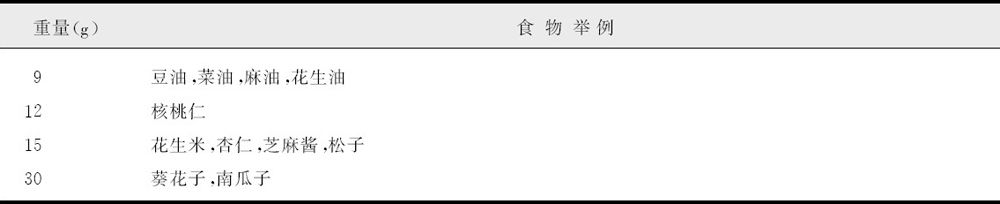
\includegraphics[width=5.89583in,height=2.59375in]{./images/Image00038.jpg}
\end{table}

区别咯血和呕血一般不难,但如患者出血急骤,量多或病史诉说不清时,有时鉴别并不容易;因此须详细询问有关病史,作细致的体格检查,及时作出诊断。

如已明确为咯血,须进一步探索其原因。引起咯血的原因很多(表\ref{tab4-2}),其中最常见的疾病是肺结核、支气管扩张、肺脓肿、支气管肺癌。此外支气管结石、肺寄生虫病、心血管疾病(特别是二尖瓣狭窄)、结缔组织病、钩端螺旋体病等也可引起咯血。

\begin{table}[htbp]
\centering
\caption{引起咯血的常见疾病分类}
\label{tab4-2}
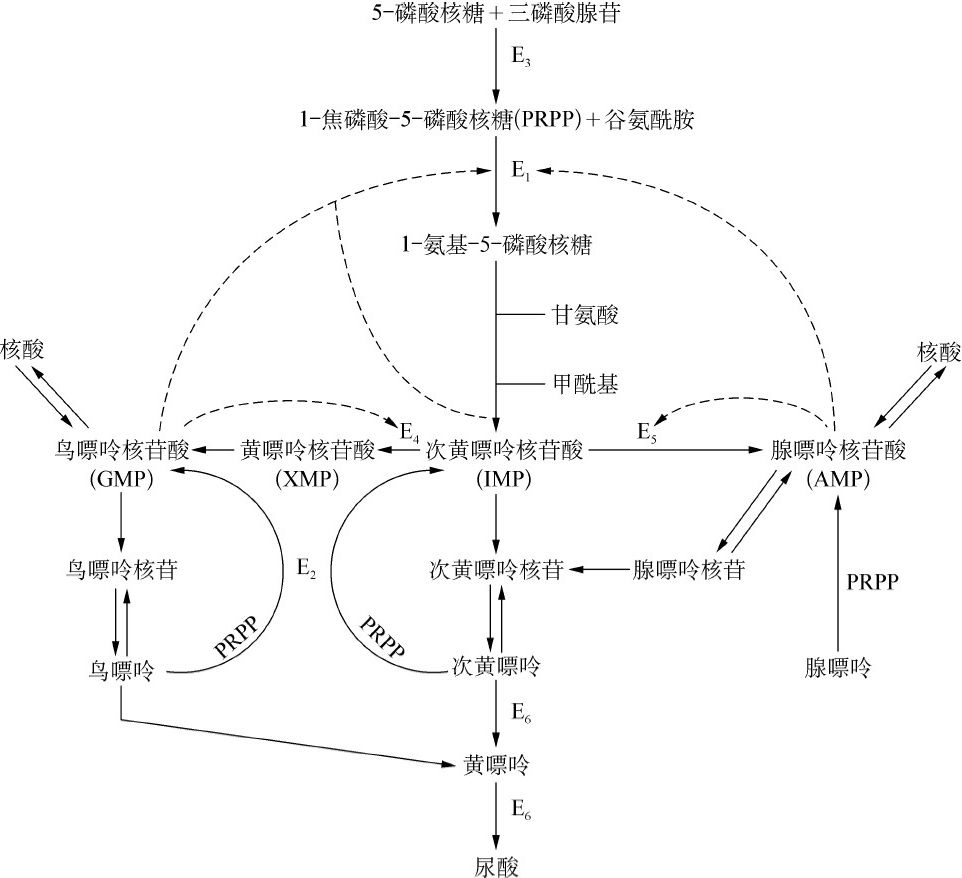
\includegraphics[width=5.89583in,height=4.80208in]{./images/Image00039.jpg}
\end{table}

如咯血量较大,应即采取急救措施,以尽早确定出血的部位。当X线检查的条件未具备时,可应用听诊法以确定。如咯血开始时一侧肺部呼吸音减弱或(及)出现湿啰音,而对侧肺野呼吸音良好,常提示出血即在该侧。气管和支气管疾病所致出血,全身症状一般不严重,胸部X线检查基本正常,或仅有肺纹理增粗;肺部病变所致出血,有比较明显的全身症状,胸部X线检查常发现病变阴影;必须指出,咯血可为全身疾病表现的一部分,临床医生必须对咯血患者做全身检查,以作出正确的诊断。

对于咯血患者,全面分析病史资料常可对咯血原因做出初步估计,同时还需要进一步做下列有关检查:

\subsection{1.病史}

须询问出血为初次或多次。如为多次,与以往有无不同。发生于幼年可见于先天性心脏病;儿童少年慢性咳嗽伴小量咯血和低色素性贫血,须注意特发性肺含铁血黄素沉着症;青壮年咯血多注意肺结核、支气管扩张等疾病;40岁以上有长期大量吸烟史(纸烟20支/
日×20年以上)者,要高度警惕支气管肺癌的可能性;年轻女性反复咯血也要考虑支气管结核和支气管腺瘤。在既往史上需注意幼年是否曾患麻疹、百日咳。在个人史中须注意结核病接触史、多年吸烟史、职业性粉尘接触史、生食螃蟹与蝲蛄史、月经史等。

细致观察咯血的量、颜色,有无带痰。肺结核、支气管扩张、肺脓肿、支气管结核、出血性疾病咯血颜色鲜红;肺炎球菌大叶性肺炎、肺卫氏并殖吸虫病和肺泡出血可见铁锈色血痰;烂桃样血痰为肺卫氏并殖吸虫病最典型的特征;肺阿米巴病可见脓血样痰呈棕褐色,带腥臭味;砖红色胶冻样血痰主要见于克雷伯杆菌肺炎;二尖瓣狭窄肺淤血咯血一般为暗红色;左心衰竭肺水肿时咳浆液性粉红色泡沫样血痰;并发肺梗塞时常咳黏稠暗红色血痰。大量咯血常由于空洞型肺结核、支气管扩张、慢性肺脓肿、动脉瘤破裂等所致;国内文献报告,无黄疸型钩端螺旋体病也有引起致命的大咯血。而痰中带血持续数周或数月应警惕支气管肺癌;慢性支气管炎咳嗽剧烈时可偶有血性痰。

详细询问伴随症状如发热、胸痛、咳嗽、痰量等。咯血伴有急性发热、胸痛常为肺部炎症或急性传染病,如肺出血性钩端螺旋体病、流行性出血热;咯血、发热同时伴咳嗽、咳大量脓痰多见于肺脓肿;长期低热、盗汗、消瘦的咯血应考虑肺结核;反复咳嗽、咳脓痰不伴有发热多见于支气管扩张。

\subsection{2.体格检查}

活动期肺结核和肺癌患者常有明显的体重减轻,而支气管扩张患者虽反复咯血而全身情况往往较好。有些慢性心、肺疾病可伴有杵状指(趾)。锁骨上淋巴结肿大在中老年患者要注意肺内肿瘤的转移。肺部闻及局限性哮鸣音提示支气管有狭窄、阻塞现象,常由肿瘤引起。肺部湿性啰音可能是肺部炎症的体征,也应考虑是否为血液存积在呼吸道所致。对咯血患者还应注意有无全身的出血表现。

\subsection{3.实验室检查}

痰检查有助于发现结核杆菌、真菌、癌细胞、肺吸虫卵等。出血时间、凝血时间、凝血酶原时间、血小板计数等检查,有助于出血性疾病的诊断。外周血红细胞计数与血红蛋白测定可推断出血的程度。外周血中嗜酸性粒细胞增多提示寄生虫病的可能性。

\subsection{4.X线检查}

对于咯血患者,除个别紧急情况不宜搬动外,均应做胸部X线检查。肺实质病变一般都能在X线胸片上显示阴影,从而及时作出诊断。如疑有空洞、肿块,或见肺门、纵隔淋巴结肿大,可加做胸部X线体层摄片或CT检查,CT还有助于发现细小的出血病灶。对疑有支气管扩张者,可做高分辨CT检查等协助诊断。对疑为支气管动脉性出血所致大咯血,必要时可行CT支气管动脉造影(CTA)或数字减影血管成像(DSA)检查,明确出血部位,后者尚可同时进行栓塞介入治疗。

\subsection{5.纤维支气管镜检查}

原因未明的咯血,尤其伴有支气管阻塞者,应考虑纤维支气管镜检查,可发现气管和支气管黏膜的非特异性溃疡、黏膜下层静脉曲张、结核病灶、肿瘤等病变,并可在直视下钳取标本作病理组织检查,吸取分泌物或灌洗液送细菌学和细胞学检查。

\subsection{6.其他检查}

先天性心脏病的诊断往往借助右心导管检查。放射性核素67镓对恶性肿瘤组织较健康组织有更大的亲和力,因而枸橼酸67镓肺部扫描可能有助于肺癌与其他肺部肿物的鉴别诊断。PET/CT对肺部肿瘤引起的咯血的诊断也有帮助。

咯血量的多少视病因和病变性质而不同,但与病变的严重程度并不完全一致,少则痰中带血,多则大口涌出,一次可达数百或上千毫升。临床上常根据患者咯血量的多少,将其分为少量咯血、中量咯血和大量咯血。但界定这三种情况的咯血量多少的标准尚无明确的规定,但一般认为24小时内咯血量少于100ml者为小量咯血;100~500ml/d者为中量咯血;>500ml或一次咯血量>100ml者为大量咯血。

临床上无异常肺部X线征象的咯血病例并不少见,诊断较为困难,其主要原因可能为:①气管或大支气管的非特异性溃疡,一般表现为小量咯血或血痰,支气管镜检查可以发现。②气管或支气管的静脉曲张,多见于右上叶支气管开口处或隆突部分,常引起大咯血,无痰,可经支气管镜检查而发现。③肺动脉瘤、支气管小动脉粥样硬化破裂,肺动静脉瘘破裂。④小块肺栓塞,常不易发现,一般有心脏病、下肢深静脉血栓形成、外伤史、长时间卧床或处于产褥期病史。⑤钩虫蚴、蛔虫蚴、血吸虫毛蚴、比翼线虫在肺内游移引起咯血。⑥早期支气管肿瘤,轻度支气管扩张、支气管结核,肺结核早期等。纤维支气管镜的广泛应用,结合胸部X线检查大大提高咯血病因的确诊率,国内一组917例经胸部X线与纤维支气管镜检查而确定的咯血病因如表\ref{tab4-3}所示:\footnote{*既有临床表现又有X线表现}

\begin{table}[htbp]
\centering
\caption{917例咯血的病因分析(X线诊断与纤支镜诊断比较)}
\label{tab4-3}
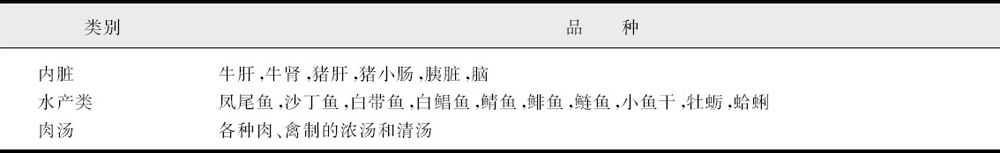
\includegraphics[width=5.91667in,height=3.58333in]{./images/Image00040.jpg}
\end{table}

由表\ref{tab4-3}所示,有部分咯血患者虽经X线和纤维支气管镜检查,仍未能发现阳性结果,且患者亦无引起咯血的全身性疾病,此类咯血可称为特发性咯血。但仍有可能在以后随诊中,在这类“特发性咯血”患者的一部分中,检出呼吸系统疾病。

国内曾有报告一组390例胸片无明显异常的咯血患者,作纤维支气管镜检查,结果发现肺癌16例(4.1\%)、支气管结核2例、支气管腺瘤1例,支气管囊性静脉曲张出血l例。作者认为咯血患者40岁以上,吸烟指数(吸烟年限×每天吸烟支数)>400,咯血时间长,且为痰血而非纯咯血者,尤须警惕肺癌的可能性。

X线胸片是咯血患者的常规检查,但可能无阳性发现。X线胸片正常的咯血患者应进一步作病因学诊断。有作者推荐应先作CT检查,以期发现潜在的肺部病灶,并有助于以后做纤维支气管镜检查时,有目标地进行刷检、活检取材,提高咯血的病因学诊断率。

\protect\hypertarget{text00057.html}{}{}

\subsection{12.1 气管和支气管疾病}

\subsubsection{一、急、慢性支气管炎}

急、慢性支气管炎患者有时也可咯血,一般为小量或痰中带血,不需治疗,可在数天内自行停止,但易于再发。如出血量大,需注意其他原因。本病的咯血与支气管炎症加剧有一定的关系,故咯血前常有病情加重的表现。慢性支气管炎患者发生持续的小量咯血时,须小心寻找其他原因,特别是支气管肺癌。

\subsubsection{二、非结核性支气管扩张}

非结核性支气管扩张可分为原发性与继发性。继发性者是由于支气管内或支气管外阻塞,引起支气管腔与支气管壁的感染,从而损害支气管壁的各层组织所引起。原发性支气管扩张则无明显的引起支气管阻塞的因素,但多数有肺炎病史,特别是麻疹、百日咳、流感等所继发的支气管肺炎史。

咯血是非结核性支气管扩张的常见症状,文献报告约90\%患者有不同程度的咯血,并作为提示诊断的线索。咯血可从童年即开始,常伴有杵状指(趾)。

此病的咯血有两种不同表现:

\paragraph{1.小量咯血}

在经常有慢性咳嗽、脓痰较多情况下,同时有小量咯血;有时在咯血前先有咳嗽较剧烈的一段感染加重阶段。因感染导致支气管内肉芽组织充血及损伤小血管而出现咯血。

\paragraph{2.大咯血}

由于支气管有炎症病变,血管弹性纤维被破坏,管壁厚薄不匀或形成假血管瘤,加上炎症影响,易破裂引起大咯血。咯血量每次达300~500ml以上,色鲜红,常骤然止血(因此类出血常来自支气管动脉系统,压力高,而动脉血管壁弹性好,收缩力强,故可较快止血)。

患者病程虽长,但全身情况尚好。咳嗽和咳痰也为常有的症状,咳嗽可轻微,也可相当剧烈;咳嗽和咳痰常与体位改变有关,如在晨起或卧床后咳嗽可加剧,咳痰增多。痰量可为大量,每天达数百毫升(湿性型)。痰液静置后可分为三层:上层为泡沫状黏液,中层为较清的浆液,下层为脓液及细胞碎屑沉渣。有些患者痰量甚少(干性型),如合并感染,痰量随之增多,并有发热、咯血等。

支气管扩张的好发部位是下肺,以左下叶较右下叶为多见,最多累及下叶基底段,病灶可延伸至肺边缘。病变部位出现呼吸音减弱和湿性啰音,位置相当固定,体征所在的范围常能提示病变范围的大小。

胸部X线平片检查不易确诊本病。国内一组84例非结核性支气管扩张中,只1/3病例在胸部X线平片上有少许的征象,大部分甚至没有任何改变。胸部X线平片检查对排除慢性肺脓肿及慢性纤维空洞型肺结核颇有帮助。如患者有支气管扩张的临床表现,X线胸片又显示一侧或双侧下肺纹理增粗、紊乱以及蜂窝状小透亮区,或见有液平面则支气管扩张的可能性最大,胸部CT检查可确定诊断,并对明确病变部位及决定治疗方案有重要意义。

全内脏转位、支气管扩张、鼻窦病变三联症,又称Kartagener综合征,国内有少数病例报告。此综合征有咳嗽、咳痰、咯血等症状。咯血可从童年开始,反复发作,量不多。

\subsubsection{三、结核性支气管扩张}

结核性支气管扩张的症状因肺内结核病灶的情况而定,如肺结核病灶不严重,则可无明显症状。有时或可闻及少许干、湿性啰音。X线胸片上显示病灶似已硬结,而患者仍有或多或少的咯血,应考虑结核性支气管扩张的可能性。国内一组64例患者中,发病大多在30岁以上,90\%有咯血(痰中带血或大量咯血)。病灶部位大都在两肺上叶,尤以右上叶的后段、左上叶的尖后段多见。

结核性支气管扩张与非结核性支气管扩张的鉴别见表\ref{tab4-4}。

\subsubsection{四、支气管结核}

支气管结核一般为继发性,原发性者罕见。患者大多有咯血,其他常见症状为阵发性剧烈咳嗽、喘鸣、阵发性呼吸困难等。有时轻度动作即可引起呼吸困难与发绀。如发生支气管阻塞,则引起突然的发热、痰量减少,而阻塞解除后痰量突然增加,体温也下降。

\begin{table}[htbp]
\centering
\caption{结核性与非结核性支气管扩张的鉴别要点}
\label{tab4-4}
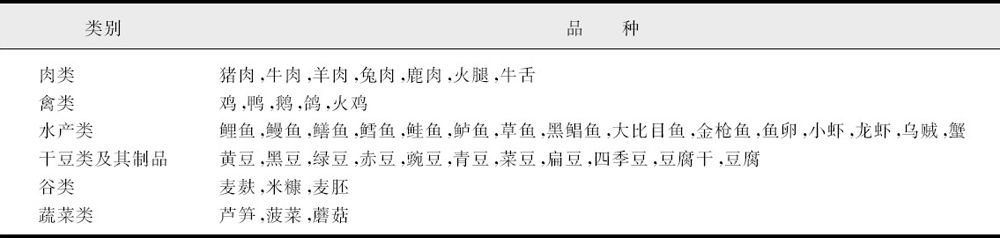
\includegraphics[width=5.94792in,height=1.65625in]{./images/Image00041.jpg}
\end{table}

支气管结核是发生于气管、支气管黏膜或黏膜下层的结核病变。据国内报告,肺结核合并支气管结核者占23.6\%~57.1\%。患者以青壮年为多,文献报告女性罹患多于男性,常发生于慢性纤维空洞型肺结核、慢性血行播散型肺结核、支气管淋巴结结核、浸润型肺结核及干酪样肺炎等基础之上。这些患者有下列情况提示有支气管结核的可能:①反复小量咯血或血痰而X线胸片未见明显病变者;②药物难以控制的刺激性咳嗽;③有喘鸣音;④有不同程度的呼吸困难而不能用肺实质病变解释者;⑤肺无明显病变而痰结核菌屡为阳性;⑥肺内有新播散病灶而不能用其他原因解释;⑦肺结核并发肺不张;⑧某些肺野空洞:在萎陷疗法后产生的张力性空洞;空洞时大时小;出现圆形、薄壁空洞;肺门附近的空洞等。

支气管结核的确诊须依靠纤维支气管镜检查。如临床症状典型,虽纤维支气管镜检查阴性,也不能除外此病的存在。

近年国内一组单纯气管、支气管结核病28例报道,误诊颇多,原因为:①胸片无异常发现;②胸片虽出现局限性肺气肿、肺纹理密集、肺纹理粗乱、叶间胸膜影移位等异常表现,但又非特异性而未加注意。作者建议对干咳、胸闷、喘息、咳黏液痰或咯血患者,经抗感染及对症治疗2周未见好转时.应及早作纤维支气管镜检查,镜下刷检涂片染色找抗酸杆菌,或钳取组织做病理检查。镜下所见仍疑似结核而实验室检查阴性时,2周后应再做纤维支气管镜检查。

目前将刷检标本或支气管肺泡灌洗液进行PCR检测结核分枝杆菌,可大大提高病原学诊断率。

结核感染T细胞斑点(T-SPOT.TB)试验是近年来的一项新诊断技术,通过检测外周血分泌γ-干扰素的T淋巴细胞数量来诊断结核感染,具有较高的特异性和敏感性,且不受卡介苗接种和环境分枝杆菌感染的影响,在肺结核的筛查和诊断中有较好的应用价值。

\subsubsection{五、支气管结石}

本病的特点为反复咯血,而肺部除有钙盐沉积之外,无其他原因可解释。患者或曾有咳出结石史。咯血通常为小量,但有些患者可有大咯血。X线检查发现有支气管结石阴影,以右中叶根部较为多见,结石远端可发现有阻塞性肺不张或肺部感染,CT检查可见支气管阻塞远端有钙化影。纤维支气管镜检查可帮助诊断。支气管结石常由肺结核病灶钙化引起。X线胸片上如炎症病变相应部位有钙化结节,在炎症消退后而咯血不断者,则支气管结石的可能性甚大。

据国内一组20例的报告中,以咯血为主要症状者占95\%,其中威胁生命的大咯血占40\%。误诊率60\%。并发症(占85\%)表现为肺不张、支气管扩张、阻塞性肺炎等。但手术治疗效果好。X线断层摄片、胸部CT和纤维支气管镜检查等综合检查对诊断有较大帮助。

\subsubsection{六、原发性支气管肺癌(肺癌)}

本病大多见于40岁以上男性,文献报告有咯血者占50\%~70\%,国内一组141例报告中,第一个月内出现咯血者有38.3\%。中央型肺癌较周围型肺癌易引起咯血。癌组织内小血管较多,患者又常有刺激性咳嗽,易引起癌组织损伤而致出血。其特点是痰中带血或小量咯血多见,而大量咯血少见,但晚期可有致命性大咯血。咳嗽是较常见的早期症状,无痰或有少量的白色黏液痰,可伴有胸痛。间断的或持续的小量咯血,对提示此病的诊断有重要意义。痰中可混有小颗粒状灰白色坏死组织,其中较易找到癌细胞。X线胸片、纤维支气管镜、胸部CT及活组织病理检查有助于诊断。

国内一组确诊肺癌患者1105例中,纤维支气管镜下直接见到肿瘤病灶(直接征象)者638例(57.7\%),只见肿瘤间接征象,即支气管黏膜改变者412例(37.3\%)。肺癌多见于段以上的支气管(中央型肺癌约占3/4),有些病例第一次活检及刷检均未能确诊,需做第二次,偶尔还要第3~4次检查。当发现有间接征象的可疑病例,应尽可能多部位活检多取标本,甚至看到癌体也应多点活检。

\subsubsection{七、支气管类癌}

支气管类癌罹患多为中年人,男女性别无差异,生长慢,具有恶性程度低和较少发生转移的特点。早期症状常为咯血,术后长期生存率较高。国内一组17例报告中,患者40岁以下者占64.7\%,中央型12例,周围型5例,2例有支气管旁淋巴结转移,主要临床表现为咳嗽、咳痰、咯血或痰中带血、发热和反复发作肺部炎症。临床上本病易误诊为肺癌、结核球或良性支气管肿瘤。X线检查与纤维支气管镜下活检对诊断帮助较大。

\subsubsection{八、良性支气管瘤}

良性支气管瘤少见,发病多在30~40岁之间。全身情况良好的中年患者如有反复的小量咯血或痰中带血,或类似哮喘发作,或屡次发作的呼吸道阻塞及感染症状,应考虑此病的可能。由于肿瘤生长缓慢,临床症状可延续多年。早期可无症状,或仅有气喘、干咳,有时甚至被误诊为支气管哮喘。肿瘤逐渐增大而堵塞支气管时,可发生相应肺叶的肺不张,并在肿瘤的远侧发生感染与支气管扩张。X线体层摄片、胸部CT,可了解较大的支气管内肿瘤的范围及部位,气道阻塞情况及继发性支气管扩张,对诊断有重要帮助。由于良性瘤多发生于较大的支气管内,纤维支气管镜检查的检出率可达85\%~90\%。

良性支气管瘤有腺瘤、平滑肌瘤、乳头状瘤等,此外较罕见的有纤维瘤、软骨瘤、脂肪瘤等。其中腺瘤比较多见,典型X线征象为肺门附近有圆形或类圆形阴影,密度均匀一致,边缘锐利,体层摄片或胸部CT检查更易于发现;由于多数腺瘤位于主支气管或肺叶支气管内,纤维支气管镜检查易作出诊断。

\protect\hypertarget{text00058.html}{}{}

\subsection{12.2 肺部疾病}

\subsubsection{一、肺结核}

咯血是肺结核患者常见的症状,且常为提示此病诊断的线索。咯血量多寡不一,少可仅为痰中带血,多则一次可达500ml以上,血色鲜红。咯血与结核病变的类型有一定关系,多见于浸润型肺结核、慢性纤维空洞型肺结核、干酪样肺炎,而少见于原发综合征(原发型肺结核)和急性血行播散型肺结核。咯血严重程度并不一定与病灶大小成正比,小的病灶可有较多的咯血,而病灶广泛的也可无咯血。出血量常和血管损害程度有关,血管壁渗透性增高所致的咯血,出血量少,但持续时间较长;小血管的破裂则多引起小量出血,这往往由于慢性活动性肺结核所致;大咯血多为肺动脉分支破损所致,其中以空洞内形成的动脉瘤破裂所致的大咯血多见,此类出血来势甚急,而由于洞壁纤维化不易收缩止血,或血凝块虽能填塞空洞压迫血管暂时止血,但又可因血块溶解而再次出血。

肺结核患者以青壮年占大多数,不少患者以咯血为初发症状而就诊。咯血之后常有发热,是由于病灶播散及病情发展所致。患者常同时出现疲乏、纳差、体重减轻、午后潮热、盗汗、脉快和心悸等全身中毒症状。

肺结核的诊断主要依靠症状、体征、X线胸片和痰结核菌检查。如在青壮年人一侧肺尖部经常听到湿性啰音,又有上述全身性中毒症状,则支持活动性肺结核的诊断。X线胸片是诊断肺结核的重要方法,可以发现早期轻微的结核病变,确定病灶的范围、部位、形态、密度、与周围组织的关系,判断病变的性质、有无活动性、有无空洞、空洞大小和洞壁特点等。因此,定期进行胸部X线检查能及早发现病灶,有助于早期治疗。

痰结核菌检查阳性可确诊为肺结核,且可肯定病灶为活动性。但痰结核菌阴性并不能否定肺结核的存在,对可疑病例需反复多次痰液涂片检查,如有需要,可采用浓集法、培养法、PCR法等,在咯血前后,因常有干酪性坏死物脱落,此时的痰菌阳性率较高。

长期被误诊为肺结核咯血的肺部疾病并非少见,文献报道有支气管扩张、支气管囊肿、肺癌、肺脓肿、肺吸虫病等。

年轻患者反复咯血,痰结核菌检查阴性,全身情况较好,而病灶又处于中、下肺野,用一般抗菌药物治疗能改善炎症表现者,则可认为是非结核性支气管扩张,胸部CT检查有助于确定诊断。支气管囊肿在胸部平片及透视下一般可确定诊断。非结核性支气管扩张或支气管囊肿合并普通细菌感染时,其症状的出现通常较早,可追溯到童年时期,特别是在患麻疹、百日咳之后常有咯血及呼吸道炎症症状,其与肺结核病的鉴别是前两者在长期的病患过程中,全身一般状况仍较好,无结核病的全身中毒症状,可伴有杵状指(趾),痰结核菌阴性。

肺癌被误诊为肺结核者颇为常见。在下列情况下,应考虑肺癌的可能:①年龄在40岁以上,尤其是长期重度吸烟的男性患者,新近出现反复的咯血或持续的痰中带血,或近肺门处有致密的异常阴影,或出现肺不张合并感染,而多次痰液检查未发现结核菌者,应首先考虑肺癌的可能;但痰中结核菌阳性也不能除外肺结核与肺癌并存。②肺癌组织内部发生坏死破溃,坏死组织排出后形成空洞,其X线征象可酷似结核性空洞。但癌性空洞常呈偏心性,其内侧壁凹凸不平,外缘多呈毛刺状、分叶状,常无病灶周围卫星灶,多次痰结核菌检查阴性,经规律的抗结核治疗无效,病灶逐渐增大,这些均可与肺结核鉴别。③肺癌和肺结核并存,肺癌可发生在陈旧性肺结核瘢痕的基础上,而肺癌又能促使结核病灶恶化。如在陈旧性或活动性结核病灶处出现新的、致密的圆形病灶,且经积极抗结核治疗一个月后,病灶仍逐渐增大,或出现肺不张、肺门阴影增大,癌性空洞等改变,应考虑并存肺癌的可能。

\subsubsection{二、肺 炎}

在急性肺炎时,肺实质处于高度充血状态,小血管通透性增加并可发生破裂而致咯血。由于小血管可发生血栓性脉管炎,致血管腔闭塞,通常不易引起大量咯血。

肺炎链球菌肺炎的患者,痰中混有血液者并不少见,有时血量可达20~30ml,病期第2、3天转为铁锈色痰。在整个病程中均呈血性痰的甚少。

肺炎杆菌性肺炎多为砖红色稠胶样痰;化脓性链球菌肺炎咳粉红色稀痰;葡萄球菌肺炎可为血性痰、脓性痰;绿脓杆菌肺炎咯血少见,典型者咳翠绿色脓痰。军团菌肺炎少量黏液痰中可带血丝,并有发热、咳嗽、肌痛、关节痛、腹泻、蛋白尿、转氨酶升高、直接荧光抗体阳性或间接荧光抗体1∶256。肺炎支原体肺炎约1/4病例有血性痰,但绝无铁锈色痰;流感病毒性肺炎常引起反复的小量咯血。

\subsubsection{三、肺脓肿}

肺脓肿多由于吸入感染或血源性感染所引起,约50\%患者伴有咯血,常伴有大量脓痰或脓血样痰。急性肺脓肿的早期可有大量的咯血而无脓痰,但此时有寒战、高热、胸痛、血白细胞和中性粒细胞增高,提示急性细菌性感染,1周后可出现大量脓性痰。慢性肺脓肿常有大量的脓痰或脓血痰,痰量每天可达300~500ml,带臭味,痰静置分层,多数患者伴有杵状指。慢性肺脓肿常被误诊为肺结核病,前者可根据急性发病史、X线胸片见大片浓密模糊浸润阴影,脓腔内出现圆形透亮区及气液平面,痰培养可有致病菌生长以及抗菌治疗有效,一般鉴别不难。慢性肺脓肿与肺癌的区别,可根据肺脓肿过去的急性发病史、空洞的特点及痰中癌细胞检查等加以鉴别,X线胸片、纤维支气管镜、胸部CT扫描有利于诊断。癌性空洞与肺脓肿空洞、结核性空洞的鉴别参见表\ref{tab4-5}。

\begin{table}[htbp]
\centering
\caption{癌性空洞与肺脓肿空洞、结核性空洞的鉴别}
\label{tab4-5}
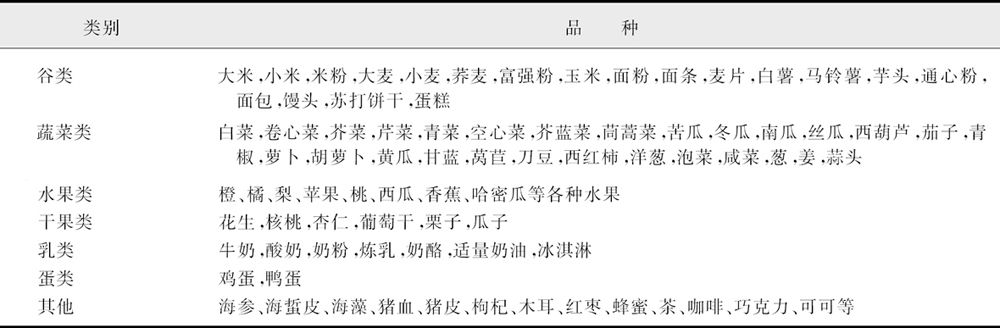
\includegraphics[width=5.97917in,height=3.53125in]{./images/Image00042.jpg}
\end{table}

\subsubsection{四、肺部真菌感染}

肺部真菌感染是最常见的深部真菌病,主要由念珠菌、曲霉、毛霉、新型隐球菌等真菌感染所致。老年、幼儿及体弱者易患此病,多为痰中带血或小量咯血。常见症状有发热、乏力、盗汗、纳差、消瘦、咳嗽、胸痛;痰的特点是量少,不同种类的真菌感染时,其痰的性状不一。肺白念珠菌感染,为胶样黏稠痰,带乳块或血丝;肺曲霉病反复咯血或咳出大量泡沫痰(可带酒味);肺新型隐球菌病则咳小量黏液性痰或血丝痰。病原学检查可找到致病菌,胸部X线检查,肺组织病理检查有助于诊断。

\subsubsection{五、肺寄生虫病}

\paragraph{1.肺阿米巴病}

阿米巴性肺脓肿为肝阿米巴病并发症之一,也可来自肠道病灶。多数起病较慢,常有发热、乏力、消瘦、咳嗽、咳痰、右下胸痛并放射至右肩,少数呈急性发病,高热、胸痛、呼吸困难等,可有肝脏肿大体征。典型的痰液呈棕褐色而带腥臭味,有助于此病的诊断。如合并出血或混合感染,可呈血性或黏液脓血痰。痰液、胸腔积液或纤维支气管镜取病变坏死组织中查找到溶组织阿米巴滋养体可确诊。

\paragraph{2.肺吸虫病}

本病有严格的地区性,患者都曾有在疫区进食未煮熟的含有肺吸虫囊蚴的石蟹或蝲蛄史。病程中常反复的小量咯血,痰血混合多呈特殊的棕黄色或铁锈色,烂桃样血痰是肺吸虫病最典型特征。早期症状有畏寒、发热、脐周隐痛、腹泻,并有乏力、盗汗、纳差,2~3周后出现咳嗽、胸痛、咯血等,患者虽有长期的反复咯血,但全身情况尚好,胸部体征多不明显,可有皮下结节。常有血嗜酸性粒细胞增多,痰中发现肺吸虫卵即能确诊,阳性率90\%以上。粪便虫卵检查、肺组织病理检查、免疫学检查、X线检查等有助于诊断。

胸部X线检查有较特别的征象,病灶多位于中、下肺野及内侧带,因病变的不同时期而有下列的表现:①早期呈边缘模糊的弥漫阴影,大小约为1~2cm;②中间期为边缘清楚、多房或单房的、实质或囊状的大小不等的阴影,多房性囊状阴影是本病的X线特征;③晚期为纤维增殖性变及硬结钙化阴影。此外,可有肺门增大、肺纹理增粗紊乱、胸腔积液或胸膜增厚等征象。对一些疑难的、不典型的病例,流行病学调查和免疫学检查,在诊断上有重要意义。

如患者有上述的流行病学史和胸痛、咳铁锈色痰等症状,血嗜酸性粒细胞增多,痰中虽未发现肺吸虫卵,而肺吸虫抗原皮内试验阳性,并已除外血吸虫病、华支睾吸虫等感染时,则大致可作出肺吸虫病的临床诊断,并应进行特效药物(如吡喹酮)的诊断性治疗;如疗效显著,可进一步确立诊断。肺吸虫病主要须与肺结核相鉴别(表\ref{tab4-6})。

\begin{table}[htbp]
\centering
\caption{肺吸虫病与肺结核鉴别}
\label{tab4-6}
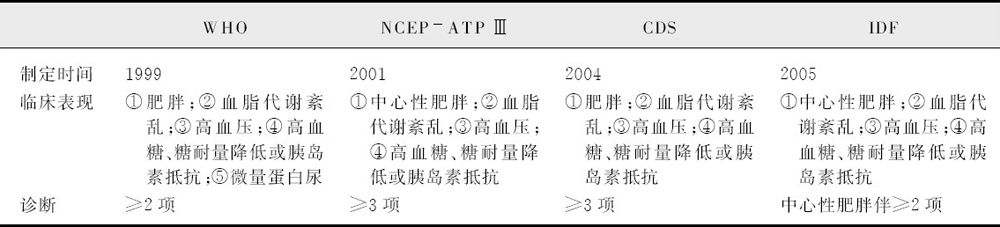
\includegraphics[width=5.94792in,height=4.91667in]{./images/Image00043.jpg}
\end{table}

在四川及福建发现的肺吸虫病,临床表现较特别,其症状轻,咯血量较小,痰中虫卵检出率较低,有游走性皮下结节者甚多(多分布于胸壁及上腹壁),血中嗜酸性粒细胞显著增多。

国内报道肺吸虫病误诊率较高。主要原因是由于肺吸虫病临床表现及X线胸片大多无特异性,且典型的游走性皮下结节,肺空泡、结节和隧道线条等X线表现又少见。一组报道34例肺吸虫病在入院前全部误诊为肺结核。

由于肺吸虫病免疫学诊断的敏感性和特异性高,且简便易行,在流行区内患者有生食石蟹或蝲蛄史,而反复出现咳嗽、咯血或痰中带血、发热等症状,应即作肺吸虫抗原皮内试验,上述一组误诊为肺结核的34例患者,肺吸虫抗原皮内试验全部为1∶2000以上阳性。应用混合单抗双抗体夹心ELISA法诊断疑难肺吸虫病,效果更佳。

\paragraph{3.肺包虫病}

肺包虫病是棘球绦虫的幼虫(棘球蚴)寄生于人体肺内所引起,主要流行于畜牧区,以青壮年农民和牧民为主,早期可无症状。当包囊肿大破裂时可出现咯血或痰中带血,并可咳出类似粉皮样的角皮膜;合并感染时则出现咳嗽、咳痰、胸部不适,或胸痛及劳力后气促等症状。可有肝脏或其他部位囊肿征象。囊肿破裂,囊液亦可阻塞气管而引起窒息。X线胸片或CT扫描有助于诊断,可显示包虫圆形或卵圆形,略呈分叶状阴影,边缘清晰,密度均匀,壁可钙化,阴影随呼吸而变形;包虫囊壁破裂,空气进入,则顶部呈现半月形透亮带。包虫抗原皮内试验及补体结合试验对本病有重要的诊断意义,阳性率可达90\%以上。此外,痰检查、B超检查、放射性核素扫描等对诊断也有帮助。

\subsubsection{六、恶性肿瘤的肺转移}

恶性肿瘤转移至肺部时,可引起咯血。较常发生肺部转移的恶性肿瘤有鼻咽癌、乳腺癌、食管癌、胃癌、肝癌、结肠直肠癌、前列腺癌、睾丸畸胎瘤、精原细胞瘤、绒毛膜上皮细胞癌、恶性葡萄胎及类癌等。以绒毛膜上皮细胞癌、睾丸畸胎瘤和恶性葡萄胎的肺转移的咯血发生率最高。对成年女性原因未明的咯血,患者阴道曾排出水泡样胎块,或兼有流产后持续的不规则阴道出血,应考虑恶性葡萄胎或绒毛膜上皮细胞癌的可能性,尿妊娠诊断试验有助于此病的诊断。

转移性肺恶性肿瘤常为多发,但也可为单发,后者较少见。X线胸片显示多发性肺转移肿瘤的形态多为圆形、卵圆形或粟粒状阴影,大小相仿,边缘不整,发展较快。转移性肺恶性肿瘤原发病灶的诊断有时不易,须设法寻找。

\subsubsection{七、肺梅毒}

本病极为少见,国内仅有二例感染报告,均有咯血。病程进展缓慢,往往有咳嗽、咯血、胸痛等症状,虽然X线胸片显示下肺野呈大片状实质模糊阴影,但全身情况良好。诊断须依据梅毒感染史、梅毒血清反应阳性与驱梅治疗的疗效。肺梅毒须与其他肺部疾病相鉴别,特别是肺结核病。

\subsubsection{八、肺囊肿}

肺囊肿可区分为先天性与后天性两类,以前者较为多见,后者是由肺部感染性疾病或寄生虫所引起。多发性先天性肺囊肿常伴有支气管扩张,多在儿童期出现症状,其临床表现与支气管扩张相似,患者往往因突然小量咯血或痰中带血而就诊,由于病变多位于中、上肺,引流较好,较少出现发热。X线胸片检查呈圆形透亮影,其壁菲薄而整齐;多发者大小不一,可分布于任何肺野,但以中、上肺野较多见。

多发性先天性肺囊肿需与支气管扩张鉴别。肺囊肿继发感染时可出现大片状模糊阴影,类似浸润性肺结核,但经抗生素治疗后感染较快消退,而有别于肺结核。肺囊肿合并感染时,其临床症状和X线胸片的改变与肺脓肿相似,需加以鉴别。

国内曾报告一组82例的成年患者中,52例(63.4\%)有咯血,多数在200ml以下,认为如有下列情况应考虑本病:①肺部阴影长期存在;②阴影在同一部位反复出现;③无播散灶;④阴影新旧程度一致;⑤肺门及纵隔淋巴结不大。患者虽反复咯血而无结核中毒症状。胸部CT检查有助于对本病的诊断。

近年肺囊肿有一组38例报告,发病常在青少年期,5例初发年龄在10岁以下。全部患者(38例)在院外均被误诊为肺结核。初发症状以咯血或痰中带血多见(21/38),咳嗽、咳痰、发热次之。6例无症状患者经体检而发现本病。21例有长期反复出现咯血或痰中带血史,最长者达20年。

肺囊肿的胸部X线表现常缺乏特征性。作者认为以下几点有利于肺囊肿的早期诊断:①发病年龄在30岁以下,特别是男性,有反复咯血或痰中带血、咳嗽、发热史。②动态观察X线胸片阴影的形态变化不大,无肿瘤的淋巴结、淋巴道远处转移的改变。③结核菌素试验阴性或经积极的抗结核治疗无效。④胸部X线显示其病变虽无固定部位但与支气管走向有关;虽经反复感染但病变部位固定不变;在非囊肿部位不出现新的病灶。⑤有条件时应作高分辨胸部CT检查加以鉴别。⑥经上述不能确诊时应考虑肺活检或外科手术探查。

\subsubsection{九、尘 肺}

包括硅沉着病和其他尘肺,是由于长期吸入某种粉尘所致的以肺实质弥漫性纤维病变为主的疾病。主要发生于从事粉尘作业的工人,可有慢性、顽固性咳嗽,咳泡沫状痰、咯血或痰中带血,气短和胸痛。早期症状不明显,常为干咳或带黏稠痰,晚期咳嗽加重,痰多,如合并肺结核或支气管扩张,可反复大咯血。晚期病情重,有发绀、杵状指、肺气肿、肺源性心脏病等表现。胸片可见中、下肺野呈网状、条索状或结节状阴影改变,肺门淋巴结肿大。其诊断主要依据为职业病史、临床表现、胸部X线征象及肺功能检查。

硅沉着病合并肺结核比无硅沉着病的发病率高4~5倍,其特点是肺结核的发生率和严重程度与硅沉着病的发展程度成正比,硅沉着病愈严重,其并发肺结核的可能性愈大,肺结核病的病变发展也愈迅速,病情愈严重。石棉肺合并肺结核比较少见,但合并肺癌者却较多。

\protect\hypertarget{text00059.html}{}{}

\subsection{12.3 肺血管及其他循环系统疾病}

\subsubsection{一、肺血栓栓塞症}

肺血栓栓塞症是肺栓塞的最常见类型,占肺栓塞中的绝大多数,多继发于右心或体循环深静脉系统的血栓形成,偶尔也见于肺动脉炎、感染性心内膜炎等病例中,是以各种栓子阻塞肺动脉系统为其发病原因的一组疾病或临床综合征。主要症状为呼吸困难及气促、胸痛、小量咯血(大咯血少见)、咳嗽、心悸、发热等。心瓣膜病(特别是合并心房颤动)患者发生咯血、未能解释的短期发热时,须考虑肺血栓栓塞症的可能。X线胸片可显示区域性肺纹理变细、稀疏或消失,肺野透亮度增加;也可显示肺组织的继发改变,如肺野局部的片状阴影,尖端指向肺门的楔形阴影,肺不张或膨胀不全,有肺不张侧可见横膈抬高。X线胸片对鉴别其他胸部疾病有重要帮助。螺旋CT、放射性核素肺通气/血流灌注扫描、磁共振显像(MRI)及肺动脉造影都是肺血栓栓塞症的重要确诊方法。

\subsubsection{二、肺动脉高压}

肺动脉高压可由许多心、肺和肺血管疾病引起,根据发病的原因是否明确,曾被习惯性分为“原发性”和“继发性”肺动脉高压。2008年世界卫生组织第4届肺动脉高压会议重新修订了肺动脉高压分类,目前按照病因或发病机制、病理与病理生理学特点分为五个大类:①动脉性肺动脉高压;②左心疾病所致肺动脉高压;③肺部疾病及(或)低氧所致肺动脉高压;④慢性血栓栓塞性肺动脉高压;⑤未明多因素机制所致肺动脉高压。继发性肺动脉高压较原发性肺动脉高压常见,早期临床表现以基础疾病如慢性支气管炎、COPD等的临床表现为主,晚期以右心功能不全的表现为主。原发性肺动脉高压是一少见病,被世界卫生组织改称为“特发性肺动脉高压”,是一种不明原因的肺动脉高压。早期通常无症状,仅在剧烈活动时感到不适;随着肺动脉压力的增高,可逐渐出现呼吸困难、胸痛、头晕或晕厥、咯血。咯血量通常较少,有时也可因大咯血而死亡。其他症状还包括疲乏、无力,雷诺现象,声嘶(Ortner综合征)等。胸部X线检查、超声心动图和多普勒超声检查、放射性核素肺通气/灌注扫描、右心导管术、肺活检都对诊断有重要的作用。

\subsubsection{三、肺动静脉瘘}

肺动静脉瘘是先天性肺血管的血管瘤样畸形,也可为获得性,临床上少见。可有咳嗽、间歇小量咯血、发绀、杵状指(趾)及红细胞增多症。体格检查可发现在相应胸壁部位触及震颤,闻及来回性血管杂音。X线胸片和胸部CT在诊断上起重要作用,可见边缘整齐、密度均匀的圆形或卵圆形阴影,多位于中下肺野,且与肺门之间有条索状阴影,病变无钙化,无空洞形成。肺动静脉瘘发病常与遗传性出血性毛细血管扩张症有关,可误诊为肺结核球或支气管肺癌,肺动脉造影可协助明确诊断。

\subsubsection{四、单侧肺动脉发育不全}

本病少见,患者大多有不同程度的咳嗽、咳痰、痰中带血、胸痛、气促等表现,体格检查可发现患侧胸廓扩张稍受限、语颤及呼吸音减弱、多可听到干、湿性啰音,可被误诊为肺气肿、气胸、支气管扩张等。诊断主要依靠胸部X线检查,尤其是胸部CT的肺动脉造影对诊断极有帮助。

\subsubsection{五、肺淤血}

常见于风湿性心脏病二尖瓣狭窄,且多发生在较严重的瓣口狭窄的慢性充血期,也可见于急性左心衰、复张后肺水肿、高原性肺水肿等,多表现为痰带血丝、小量咯血或咳出粉红色泡沫样痰。结合心脏病史、胸腔快速抽液(气)及快速登山等病史,心尖部舒张期隆隆样杂音,超声心动图和多普勒超声检查等可作出诊断。二尖瓣关闭不全较少引起咯血。

\subsubsection{六、高血压}

在恶性或急进型高血压,由于血压持续增高时,可引起肺毛细血管破裂而出现咯血。也可由于并发急性肺水肿而咳粉红色泡沫样痰。

\subsubsection{七、先天性心脏病}

某些有血液分流的先天性心血管病如房间隔缺损、室间隔缺损、艾森曼格综合征等,均可伴有显著的肺动脉高压,由此可引起咯血。

\protect\hypertarget{text00060.html}{}{}

\subsection{12.4 全身性疾病及其他原因}

\subsubsection{一、急性传染病}

1.肺出血型钩端螺旋体病
肺出血型钩端螺旋体病也称钩端螺旋体性出血性肺炎,是钩端螺旋体病的严重类型,如不注意常易误诊。钩端螺旋体病以夏秋季多发,以青壮年为主,从事牧、渔业劳动者发病率高,大多起病急骤,症状主要有畏寒或寒战、高热、头痛、全身肌肉酸痛、衰弱无力、眼结膜充血、腓肠肌疼痛、淋巴结肿大,多在毒血症过程中出现心悸、烦躁、呼吸和心律逐渐增快。初为痰中带血,以后咯血量增多。严重的肺弥漫性出血型者,可引起致命的大咯血,其特点是发生突然、发展迅猛,临终时多数患者出现从口鼻涌出大量血液,立即窒息而死。X线胸片和胸部CT显示双侧肺野斑片状模糊阴影,以中、下肺野尤其显著。需与其他原因的肺炎、肺结核鉴别。病原学和血清学检查有助于明确诊断。

2.流行性出血热
由汉坦病毒引起,经呼吸道、消化道、母婴、虫媒及动物源传播,流行季节以3~5月份或5~7月份以及11月份至次年1月份间为高峰,青壮年多见,主要损害全身小动脉和毛细血管。患者起病急,典型病例具有发热、出血与肾损害三大主要特征以及发热期、低血压休克期、少尿期、多尿期和恢复期五期经过。其主要临床表现为发热、头痛、腰痛、眼眶痛、口渴、呕吐、酒醉貌、球结膜充血水肿,皮肤和黏膜广泛出血、鼻出血、咯血、呕血、便血、血尿,软腭及腋下有出血点,肾区有叩击痛。早期外周血白细胞正常或偏低,有尿蛋白,尿红、白细胞及管型改变;肾功能损害,约有半数出现肝功能损害。特异性血清学试验有助于确诊。

\subsubsection{二、血液病}

某些血液病如血小板减少性紫癜、白血病、再生障碍性贫血、血友病等均可出现咯血,与原发病有关。除咯血外,尚伴有其他部位的出血倾向。血常规、骨髓细胞学检查、血小板功能与凝血因子检查可确诊。

\subsubsection{三、白塞病(Behcet disease)}

本病由病毒感染、遗传因素、免疫功能及体内微量元素异常等因素引起。初发年龄主要是16~40岁的青壮年,以女性多见。基本病变是血管炎,可累及毛细血管和细小动静脉,可因肺部血管受累而反复咯血,多为小量咯血,也有因肺脉管炎而引起多发性肺栓塞。主要的临床表现为反复发作的口腔黏膜、舌尖及其边缘、齿龈、上下唇内侧等处的痛性小溃疡;外生殖器损害与口腔基本相似;眼部损害主要为结膜炎、角膜炎、虹膜炎、视网膜炎,其他表现有皮肤损害、消化道损害、关节损害及神经系统损害等。活动期多有血沉、黏蛋白、唾液酸、α2球蛋白增高,部分患者血浆铜蓝蛋白及冷球蛋白阳性。本病并发肺脉管炎引起咯血时的胸部X线表现,可类似肺炎支原体肺炎、肺部转移癌,或出现大片密度增高的圆形阴影。病理学检查及有关脏器病变的相应检查有助于诊断。针刺反应阳性是一特征性表现,若能同时检查HLA-B5,对本病的诊断更有帮助。

\subsubsection{四、结缔组织病}

该类疾病如系统性红斑狼疮、结节性多动脉炎、重叠综合征等,其发病与遗传、某些药物、物理因素、病毒感染、内分泌因素、免疫异常等有关,多见于20~40岁的女性。可有小量咯血,如伴有肺动脉受侵害,可发生大咯血。若患者有多个器官系统功能的损害,胸部X线检查见肺部有阴影,而抗菌药物治疗效果不佳时,应考虑结缔组织病伴有肺部损害的可能性。诊断结缔组织病所致的咯血时,须认真除外肺结核、支气管扩张、肺肿瘤等疾病。实验室检查和肺组织病理检查有助于诊断。

\subsubsection{五、肺出血-肾炎综合征}

国外文献曾有多例重度肺出血合并肾小球性肾炎报告,并命名为Goodpasture综合征,病因未明,也有将此病归入结缔组织病,临床上少见。此病多见于20~40岁男性,病程数月至数年,预后不良。临床经过可分为两个阶段:①肺部病变阶段,87\%~96\%以上的病例的首发症状表现为间歇的咯血,轻者为血痰,重者出现大咯血,反复出血可致贫血;病变广泛者可有呼吸困难、发绀与胸痛,X线胸片上显示短暂的弥漫性细小或大片状阴影,但X线检查也可呈阴性。②肾脏病变阶段:多数患者在咯血后数周或数月出现肾炎症状,肾脏病变表现为肾小球性肾炎,起病隐袭,当肺部病变显著时,尿检查发现蛋白尿、镜下血尿与管型尿,早期肾功能正常,当肾脏病变为进行性,尿毒症症状迅速出现,并掩盖肺部症状。X线、痰涂片、尿常规、血液检查、免疫学检查、肺功能检查都有助于诊断。肾组织活检免疫荧光检查,发现抗肾小球基底膜抗体则可明确诊断。通常由于尿毒症导致死亡。

除肺、肾两脏器之外,其他脏器很少受累。高血压少见。

\subsubsection{六、肉芽肿性多血管炎(韦格纳肉芽肿)}

是一种原因未明的综合征,被认为是机体对未知抗原的异常超敏反应所致。以30~50岁男性多见,具有上下呼吸道坏死性肉芽肿性血管炎,肾小球肾炎和小血管炎的临床表现。常有小量咯血,严重者可发生大量肺泡性出血,患者可伴有发热、乏力、纳差、关节痛、肌痛;上呼吸道症状有鼻分泌物增多、口咽部溃疡、声嘶;肺部症状有咳嗽、胸痛、呼吸困难;肾损害表现有不同程度的蛋白尿、镜下血尿或红细胞管型;其他表现可有皮肤黏膜损害、血疱、结节、红斑、结膜角膜炎、多发性神经炎、心肌炎、耳部损害。胸部X线检查表现为肺单侧或双侧多发或孤立结节影,大小不等,边界清楚,多有空洞形成,空洞壁薄而形态不规则,罕有液平存在。口咽、肺、肾组织活检及实验室检查有助于诊断,典型病例胞浆型抗中性粒细胞胞浆抗体(c-ANCA)阳性。

\subsubsection{七、弯刀综合征}

弯刀综合征为一种罕见的先天性血管畸形,其特征为右肺静脉开口于下腔静脉,X线胸片显示血管形态类似古代土耳其武土佩带的弯刀。患者常有反复咳嗽、咯血、右肺感染,易被误诊为“支气管扩张”。胸部X线检查为:①右肺发育不全;②X线检查沿右心缘的肺静脉呈弯刀样阴影;③心脏向右移位,状似右位心,据此可作出诊断。

\subsubsection{八、替代性月经}

成年女性发生与月经期相应的周期性咯血,须考虑为“替代性月经”。国内文献报告一例每次咯血都在月经周期前2~3天开始,待月经过后即能自行停止。此种异常现象罕见,原因未明,有人认为体内雌激素的周期性浓度增高,引起肺毛细血管充血、出血所致。部分患者在咯血周期前1周,应用黄体酮治疗可预防出血。此外,气管或支气管子宫内膜异位也可引起此现象,但罕见。

对此类与月经周期有明显关系的周期性咯血,须经细致检查与长期观察,而不能发现咯血

的其他原因时,方可下“替代性月经”的诊断。

(周燕斌 谢灿茂)

\protect\hypertarget{text00061.html}{}{}

\section{参考文献}

1.孙书明,等.138例咯血患者的胸部X线检查与纤维支气管镜检查对照分析.中华结核和呼吸杂志,1995,18(4):226

2.来孺牛.纤维支气管镜、螺旋CT对咯血的诊断价值.现代中西医结合杂志,2004,6:352

3.姜静波,等.CTA与DSA对支气管动脉性咯血临床应用价值的比较.医学临床研究,2012,29(7):1334-1337

4.宋美君,等.多层螺旋CT支气管动脉造影与数字减影下经股动脉支气管动脉造影在咯血诊治中的对比.中国呼吸与危重监护杂志,2012,11(4):378-381

5.胡华成,等.X线胸片正常咯血患者病因的进一步诊断.中华结核和呼吸杂志,1994,17(6):377

6.陈志烈,等.胸片无明显异常的支气管扩张症青年患者咯血的诊断与鉴别.宁夏医学院学报,2001,23
(1):28

7.林金学,等.单纯气管、支气管结核病28例临床分析.中华结核和呼吸杂志,1997,20(6):368

8.杨远,等.纤维支气管镜检讨胸片正常的支气管内膜结核.中华结核和呼吸杂志,1995,18(1):12

9.陈文彬,等.酷似肺癌的支气管结核六例.中华结核和呼吸杂志,1995,18(4):246

10.张立华,等.T-SPOT与结核菌素试验对结核病患者的临床诊断价值.中华临床医师杂志(电子版),2012,6(14):4107-4108

11.高明乐,季卫星.支气管壁内结石致大出血介入治疗1例.临床荟萃,1998,13(22):1040

12.林耀广,等.肺癌在支气管镜下的特征.中华内科杂志,1998,37(4):235

13.张逊,等.支气管类癌外科治疗11例报告.中华结核和呼吸杂志,1995,18(1):40

14.张兵,雷发国.34例肺吸虫病误诊临床分析.中华传染病杂志,1998,16(1):54

15.刘云霞,等.混合单抗双抗体夹心ELISA法诊断疑难肺吸虫病二例.中华内科杂志,1997,36(6)420

16.王维山,等.38例支气管囊肿临床及X线形态分析.中华结核和呼吸杂志,1994,17(5):314

17.易善国,等.弯刀综合征一例.中华内科杂志,1992,31(3):176

18.陈庆荣,等.Goodpasture综合征(附7例)报告及文献复习.中华肾脏病杂志,1991,7(2):93

19.毕经瑞.支气管子宫内膜异位症引起咯血1例报告.吉林医学,1998,19(6):333

\protect\hypertarget{text00062.html}{}{}


\chapter{慢性咳嗽}

咳嗽是一种保护性反射动作,能将呼吸道内分泌物或异物排出体外;另一方面也为病理性,作为呼吸系统疾病的常见症状。当耳、鼻、咽、喉、支气管、胸膜、肺等脏器,由于炎症、淤血、物理、化学或过敏等因素刺激时,通过分布于此等器官的迷走神经分支传达到延髓咳嗽中枢,引起咳嗽反射。目前已把咳嗽分成急性、亚急性和慢性咳嗽(chronic
cough),急性咳嗽定义为咳嗽持续3周以内,亚急性咳嗽为3~8周,慢性咳嗽为8周以上。能引起慢性咳嗽的疾病很多(参考表\ref{tab5-1})。诊断时须注意下列检查:

\section{(一)病史、症状、体征}

\begin{table}[htbp]
\centering
\caption{慢性咳嗽疾病的分类}
\label{tab5-1}
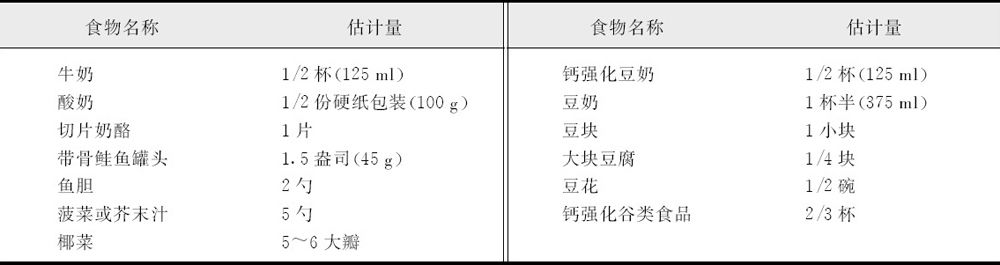
\includegraphics[width=5.90625in,height=2.69792in]{./images/Image00044.jpg}
\end{table}

识别咳嗽的不同特征有助于诊断,包括什么时候开始咳嗽?咳嗽是日间重抑或夜间重?多痰或干咳?痰液的性状如何以及咳嗽伴随什么症状?

健康状态良好的慢性咳嗽,多见慢性咽、喉炎及支气管炎,也可见于支气管扩张。经常作咽部清除动作的咳嗽和咳出黏痰,尤其起床后出现者,多为上气道咳嗽综合征(upper
airway cough
syndrome,UACS)。间歇性咳嗽伴有喘息者多为支气管哮喘。如果每年都在同一时间发作的咳嗽,可能为过敏性鼻炎。日间高声干咳,引起虚脱,伴有情感性反应者提示心因性咳嗽。呈进行性消瘦的慢性咳嗽患者,须注意为消耗性疾病,如肺结核、肺部恶性肿瘤等。

反复咳出大量脓痰者常为肺脓肿,这些患者每有醉酒、昏迷或肺部急性炎症感染病史。如于童年起病,脓痰在经过中逐渐增多,多见于支气管扩张。肺脓肿和支气管扩张的排痰量与体位改变有一定关系。伴有血痰的慢性咳嗽多见于肺结核、肺癌、支气管扩张、慢性肺脓肿、肺吸虫病、淤血性支气管炎等,有时也可见于慢性支气管炎。干咳有服用血管紧张素转换酶抑制剂(ACEI)者要注意药物诱发的咳嗽。

伴有胸痛的慢性咳嗽,常见于肺部病变波及胸膜或附近骨膜,如肺结核、支气管肺癌等。难以忍受的胸部闷痛,须注意支气管肺癌的可能。

长期与有害粉尘接触的慢性咳嗽患者,须注意尘肺的可能性。仰卧时突然发生咳嗽,口腔伴有酸味者提示胃食管反流。

细致的体格检查对60\%病例有诊断价值。体检可发现:咽充血,黏膜可伴有或没有炎性肿胀和脓性分泌物,见于鼻窦炎、上气道咳嗽综合征或过敏性疾病。双肺弥漫性吸气性湿啰音见于肺水肿或肺纤维化。呼气性哮鸣音,见于哮喘或慢性阻塞性肺疾病。散在的湿啰音咳嗽后改变或消失者见于支气管炎。固定的局限性湿啰音见于支气管扩张。肺尖部局限性小湿啰音常提示浸润性肺结核。局限性上肺野大、中湿啰音常提示空洞性肺结核。慢性咳嗽伴杵状指须注意支气管扩张,慢性肺脓肿,慢性肺性骨关节病,特发性肺纤维化。伴颈部及锁骨上淋巴结肿大须注意肺结核、肺癌。

\section{(二)痰检查}

纤维素性支气管炎痰中出现树枝状管型物。痰的细菌学检查(涂片、培养、PCR)对慢性气道和肺部炎症、肺结核、肺真菌病等的诊断有重要意义。痰细胞学检查发现癌细胞能明确肺癌的诊断,痰发现嗜酸性粒细胞增高是诊断嗜酸性粒细胞支气管炎(eosinophilic
bronchitis,EB)的主要指标。

\section{(三)器械检查}

\subsection{1.胸部X线透视及摄片检查}

能进一步确定肺部病变的部位、范围与形态,有时也可确定其性质,如肺部炎症、肺结核、肺脓肿、肺癌、肺囊肿、尘肺等。对于肺深部病变,则X线体层摄片、CT、MRI等诊断价值较大。鼻窦X线检查也有助于寻找咳嗽的病因,可以发现鼻窦炎或鼻窦积脓。胸部CT的横断面图像并无影像重叠,可发现X线胸片未能显示的病灶和小病灶,对肺间质性病变,可较早期清晰显示细小结节及网状阴影。

\subsection{2.纤维支气管镜检查}

对慢性咳嗽患者有时是必需的,可发现大气道内炎症、肿物、异物,并可做活检、支气管肺泡灌洗等。喉镜、鼻咽镜对上呼吸道病变的诊断也是必需的。胸腔镜检查对弥漫性肺疾病和胸膜疾病引起的咳嗽有重要的诊断价值。纵隔镜检查对纵隔病变有时也是必需的。

\subsection{3.支气管激发试验和舒张试验}

可诊断咳嗽变异性哮喘和其他气道过敏性疾病。最大呼气流量(PEF)变异率的测定可评价患者的气道功能状态。

\subsection{4.咳嗽敏感性检查}

通过雾化方式使受试者吸入一定量的刺激物气雾溶胶颗粒,刺激相应的咳嗽感受器而诱发咳嗽,并以咳嗽次数作为咳嗽敏感性的指标。常用辣椒素吸入进行咳嗽激发试验。咳嗽敏感性增高常见于AC、EB、GERC。

\subsection{5.24小时食管内pH监测}

可诊断胃食管反流引起的咳嗽。

\protect\hypertarget{text00063.html}{}{}

\section{13 慢性鼻、咽、喉疾病}

\subsection{一、上气道咳嗽综合征}

上气道咳嗽综合征(UACS)最早源于2006年美国胸科医师协会(ACCP)慢性咳嗽指南,用于代替过去文献中所用的鼻后滴流综合征(postnasal
drip
syndrome,PNDS),后者是指由鼻部疾病引起分泌物倒流至鼻后和咽喉部甚至反流入声门或气管,引起以咳嗽为主要表现的综合征。而UACS的定义为由鼻及鼻窦病变引起的以咳嗽为主要症状的综合征,伴或不伴PNDS,是导致慢性咳嗽的重要原因之一,咳嗽常超过8周,其患病率占慢性咳嗽的22.0\%~57.6\%。本病以慢性咳嗽、咳痰为主要临床表现,常伴有打喷嚏、鼻痒、鼻分泌物增加和鼻塞等,可有鼻后滴流感、面部疼痛及嗅觉障碍。常伴有下列体征:清喉动作、咽部黏膜充血、淋巴滤泡增生(可呈鹅卵石样外观)、咽后壁有黏性分泌物附着等。上述临床症状和体征无特异性,基础疾病的确诊尚需进一步检查。

临床诊断需综合基础疾病、咳嗽与相关症状、鼻咽检查及治疗反应进行综合诊断。我国2009年慢性咳嗽指南提出的诊断标准如下:①发作性或持续性咳嗽,以白天咳嗽为主,入睡后较少咳嗽;②鼻后滴流及(或)咽后壁黏液附着感;③有鼻炎、鼻窦炎、鼻息肉或慢性咽喉炎等病史;④检查发现咽后壁有黏液附着、鹅卵石样观;⑤经针对性治疗后咳嗽缓解。

\subsection{二、慢性咽炎}

\subsubsection{(一)慢性单纯性咽炎}

慢性单纯性咽炎是常见的咽部疾病,其突出的症状为刺激性干咳。由于咽部有瘙痒感及不适感,患者常作廓清咽部的动作,且在讲话多时症状更为显著。患者在讲话中,常须中断,并作吞咽动作以减轻症状。

咽部检查可见咽部充血,咽后壁黏膜表面可见许多扩张的毛细血管及少量淋巴滤泡增殖,咽后壁黏膜及腭弓可略增厚,分泌物可能增多,也可在咽后壁黏膜上发现有黏稠的分泌物附着。

慢性咽炎诊断较易,但病因颇多,须明确其病因,才易于防治。慢性单纯性与慢性增殖性咽炎可由急性咽炎反复发作而来,而大多数继发于上呼吸道病变,如鼻炎、鼻窦炎或口腔慢性炎症。有害粉尘、气体的吸入及烟酒过度等,均可为本病的原因。

\subsubsection{(二)慢性增殖性咽炎}

慢性增殖性咽炎的症状与单纯性咽炎相似,但较显著。

咽部检查可见咽部充血、血管扩张、软腭充血,悬雍垂也可充血、水肿,由于淋巴滤泡增殖、互相融合呈现颗粒状。淋巴滤泡增殖常阻塞咽后壁腺管开口,而致腺体分泌淤积扩大,增加了咽后壁肿胀的程度。咽扁桃体肿大可引起咽鼓管口阻塞而产生耳鸣、听力减退。患者的咽反射特别敏感,常易引起恶心。

\subsubsection{(三)慢性萎缩性咽炎}

咽干燥感是此病最突出症状,患者每于饮水后症状减轻。萎缩的黏膜上被覆痂皮时,常导致干咳、异物感及瘙痒感。

咽部检查发现黏膜苍白、干燥、菲薄而光滑,病变较重者,其上覆盖干燥黏液与痂皮。咽肌萎缩,咽腔似甚宽广。

慢性萎缩性咽炎常继发于萎缩性鼻炎,或咽手术、咽部放射性治疗之后。

\subsection{三、慢性喉炎}

\subsubsection{(一)慢性单纯性与增殖性喉炎}

慢性单纯性与增殖性喉炎的症状以声嘶为主,早期常间歇发生,且每于发音较多时出现。如病情加重,声嘶可成持续,但完全失音者尚属罕见。此外,喉部常有瘙痒、灼热、刺痛等感觉,因此患者常作干咳以减轻症状。

间接喉镜检查时,早期(慢性单纯性喉炎)患者喉部黏膜充血,声带丧失其原有色泽,且可见其上分布有扩张的血管,声带上或杓状间隙可见黏性分泌物黏附。病情加重时(即慢性增殖性喉炎),则黏膜呈暗红色,并有明显增厚,声带暗红,边缘肥厚而呈钝圆,发音时常因声带肥厚而闭合不全,喉室带因代偿活动而致增厚,其较重者可掩盖声带的一部分或全部。

\subsubsection{(二)慢性萎缩性喉炎}

此病比较少见,其主要症状为刺激性干咳,有时甚至可引起声门痉挛。咳嗽之后常咳出黄绿色的痂皮,由于咳嗽用力较猛,每使黏膜损破,以致咳出物带有血丝。声音嘶哑常于痂皮在喉中积聚较多时明显,痂皮排出后好转。由于喉肌萎缩,除声音嘶哑外,常显得软弱无力。此外喉部有灼热感及痛感。

间接喉镜检查时,可见黄绿色或黑绿色痂皮,其严重者甚至在气管内也有痂皮发现。

\subsection{四、咽结核与喉结核}

咽结核与喉结核常继发于开放性肺结核。咽结核的早期,常于水肿、苍白的咽峡、软腭或甚至舌根部出现灰白色结节;此时患者只觉咽部不适,至结节破溃形成溃疡后,才出现咽痛与吞咽痛。疼痛常很明显,患者常因此而拒食。溃疡可发生于咽部各处甚至舌部。溃疡发展缓慢、浅表、边缘不整如鼠咬状,其上附有黏液,但底部较清洁,此外患者常有发热、唾液分泌增多、消瘦及咳嗽等症状。

喉结核早期症状每为干咳及轻度声嘶,声嘶往往出现于下午或晚上,随病情加剧而声嘶越加显著,到后期不仅声嘶而且发音无力,形同耳语。喉部因分泌物积聚而常诱发持久的严重咳嗽。喉部及喉咽部疼痛明显,并常反射至耳部。吞咽痛尤剧烈,进食困难的程度较咽结核更为严重。

喉结核患者咽部黏膜显得苍白,间接喉镜检查,早期常见杓状间隙及会厌披裂后部肿胀,有时早期患者也有出现会厌肿胀的;肿胀之处黏膜均苍白,并有黏液附着于杓状间隙。声带甚至喉室带、会厌等处先后出现溃疡,其严重者喉部形态不能分辨。

\subsection{五、喉 癌}

喉癌常出现咳嗽和声音嘶哑等症状。诊断须经专科医生检查。

\protect\hypertarget{text00064.html}{}{}

\section{14 慢性支气管疾病}

\subsection{一、慢性支气管炎}

患者每年咳嗽、咳痰达3个月以上,连续2年或更长,并可除外其他已知原因的慢性咳嗽,可以诊断为慢性支气管炎。如果肺功能检测FEV\textsubscript{1}
/FVC<70\%,则为慢性阻塞性肺疾病(COPD)。引起慢性支气管炎的内因是机体及呼吸道局部抵抗力降低,外因主要是细菌或病毒感染,有害气体、尘埃的吸入,过冷、过热、过于干燥的空气的刺激以及过敏因素等。

慢性支气管炎多见于中年以上,每于冬春季加剧,夏季减轻或缓解。最突出的症状是咳嗽,尤其是清晨醒后较剧,也可在夜间加剧而致影响睡眠,咳出或多或少的脓性黏液痰,有时也可发生小量咯血。可有微热与全身不适。听诊有散在性干啰音与中、小湿啰音,但也可无明显听诊体征,后期往往并发肺气肿,X线检查可见肺纹理增粗与肺气肿等征象。

慢性支气管炎的诊断,主要应用排除法,即排除其他原因所致的慢性咳嗽而确定之。淤血性支气管炎的患者,有器质性心脏病的体征,每于劳动后或夜间平卧时咳嗽增多。支气管内膜结核,常发生于有开放性肺结核病灶的患者,表现为阵发刺激性咳嗽,有时很难制止,常有哮鸣音,痰中带血,痰抗酸染色可发现抗酸杆菌。支气管镜检查有助于诊断。支气管扩张,每以长期咳嗽、反复大量脓痰或咯血为主要症状,胸部CT、必要时支气管造影可确定诊断。长期接触有害粉尘的慢性咳嗽患者,须注意为尘肺的可能。呼吸道真菌病,其临床表现无特殊,多有长期顽固性咳嗽,咳黏稠痰或带血痰。常发生于身体衰弱或长期使用广谱抗菌素、皮质激素的患者,痰真菌检查发现真菌及菌丝,多次培养阳性及动物接种可助确诊。支气管肺癌发病多在中年以上,可有吼哮样刺激性咳嗽,常持续咯血痰,色鲜红或带褐红色,痰可找到癌细胞,胸部X线检查及支气管镜检查有助于诊断。肺吸虫病及肺包虫病,有地区性流行病学供参考,前者痰常呈铁锈色,痰中易发现肺吸虫卵;肺包虫病多见于牧区,胸部X线检查有特殊征象(参见第30节)。

\subsection{二、淤血性支气管炎}

慢性左心衰竭患者由于支气管黏膜长期淤血,常有持久的咳嗽,多在夜间平卧时或活动后加剧。体检发现两侧肺底弥漫性中、小湿啰音。国内曾见文献报道以慢性咳嗽为首发症状的左心功能不全,使用利尿剂作诊断性治疗,用利尿剂后能降低心脏前负荷,较快地解除了肺淤血和支气管黏膜水肿,从而在排尿后的5~10分钟即表现出镇咳效应。慢性心血管疾病的咳嗽,除由淤血性支气管炎引起之外,尚可能由于主动脉瘤、增大的左心房和扩大的肺动脉压迫气管、支气管,或合并支气管感染、支气管肺炎等所致。在诊断淤血性支气管炎时,上述原因须加以排除。

此外,国内曾报道一例以顽固性咳嗽为表现的室性期前收缩,患者室性期前收缩发作时出现刺激性咳嗽,经给予普罗帕酮治疗后咳嗽消失。

\subsection{三、嗜酸性粒细胞性支气管炎}

嗜酸性粒细胞性支气管炎(EB)是1989年由Gibson等首先定义的一种疾病,为一组痰嗜酸性粒细胞增多,对糖皮质激素敏感,但肺功能正常,无气道高反应性(AHR)的证据,最大呼气流量(PEF)变异率正常的非哮喘慢性咳嗽。主要症状为慢性咳嗽,或晨起咳少许黏痰。部分患者对油烟、灰尘、异味或冷空气比较敏感。目前的研究认为EB是不明原因慢性咳嗽的一个重要病因,大约占慢性咳嗽的10\%~20\%。肺功能和诱导痰检查是诊断EB主要的实验室检查。其诊断标准:①慢性咳嗽,表现为刺激性干咳或伴少量黏痰;②X线胸片正常;③通气功能正常,气道高反应性阴性,呼气峰流速日间变异率正常;④痰细胞学检查嗜酸性粒细胞比例≥2.5\%;⑤排除其他嗜酸性粒细胞增多性疾病;⑥口服或吸入糖皮质激素有效。

EB需和一些肺部寄生虫感染性疾病(如肺吸虫)相鉴别,肺部寄生虫感染也可以表现为慢性咳嗽,少数痰中可见到嗜酸性粒细胞增多,但其外周血中嗜酸性粒细胞明显增高,胸片多有异常,吸入糖皮质激素治疗无效而驱虫治疗有效。

\subsection{四、弥漫性泛细支气管炎}

弥漫性泛细支气管炎(DPB)于1969年由日本学者发现,是一种弥漫存在于两肺呼吸性细支气管区域的气道慢性炎症性疾病。至今病因尚不清楚,可能与人种、遗传因素有关。DPB的受累部位主要是呼吸性细支气管以远的终末气道,病理学特点是炎症病变弥漫性地分布并累及呼吸性细支气管壁的全层。突出的临床表现是咳嗽、咳痰和活动后气促。严重者可导致呼吸功能障碍。在有大环内酯类抗生素疗法之前,DPB多数预后不良,5年生存率只有5\%左右,而大环内酯类抗生素疗法(十四元环、十五元环大环内酯)开展以来已提高到95\%。

本病诊断标准:必备条件:①持续性咳嗽、咳痰、活动时呼吸困难;②合并有慢性鼻窦炎或有既往史;③胸部X线可见两肺弥漫性散在的颗粒样结节状阴影或胸部CT可见两肺弥漫性小叶中心性颗粒样结节状阴影。参考条件:①胸部听诊断续性湿啰音;②一秒钟用力呼气容积(FEV\textsubscript{1}
)占预计值百分比降低(<70\%)以及低氧血症(PaO\textsubscript{2}
<80mmHg);③血清冷凝集试验(CHA)效价增高(>1∶64)。确诊:符合必备条件①、②和③加上参考条件中的2项以上;一般诊断:符合必备条件①、②和③;可疑诊断:符合必备条件①和②。

本病近年国内已有报道。需要和本病相鉴别的是一些临床表现、影像学或病理改变相类似的疾病,如COPD、支气管扩张、支气管哮喘、粟粒型肺结核、结节病、癌性淋巴管炎、肺泡细胞癌、纤毛不动综合征、呼吸性细支气管炎伴间质性肺病(RBILD)和慢性外源性过敏性肺泡炎等,X线胸片、高分辨率CT(HRCT)、病理组织学检查等是主要的鉴别手段。也可通过大环内酯类抗生素进行治疗观察。

\subsection{五、咳嗽变异型哮喘}

咳嗽变异型哮喘(CVA)是以咳嗽为其唯一症状的哮喘,患者无发作性的喘息、气急,双肺无哮鸣音。目前发现约6.5\%~57\%的慢性咳嗽的真正原因为CVA。患者常常具有过敏性疾病或哮喘家族史,或同时患有过敏性鼻炎。咳嗽多为刺激性干咳,发作频繁、剧烈,下半夜咳嗽是其特征。可由于上呼吸道感染、运动、冷空气吸入以及过敏原等刺激而诱发并加重。支气管激发试验常阳性,提示气道高反应性,按照支气管炎给予止咳和抗生素治疗无效,而按哮喘给予支气管舒张剂和吸入糖皮质激素治疗可奏效。CVA患者若不能得到及时诊断及治疗,多数可逐渐发展为典型哮喘。

CVA的诊断要点为:①慢性持续性干咳达1~2个月以上,伴有夜间咳嗽或运动性咳嗽,经正规抗生素及止咳祛痰药物治疗无效;②气道呈高反应性;③泼尼松试验阳性或支气管舒张剂能显著改善咳嗽症状;④除外其他导致慢性干咳的病因。

\subsection{六、变应性咳嗽(atopic cough)}

变应性咳嗽是1992年由日本的学者Fujimura首先定义的一种疾病诊断,表现为变应性非哮喘性慢性干咳,支气管扩张剂无效,肺功能正常,无气道高反应性的证据,峰流速变异率正常,抗组胺药或糖皮质激素治疗效果良好。本病与变应性咽喉炎、EB、感冒后咳嗽的关系及异同还有待进一步明确。其主要临床表现为刺激性干咳,多为阵发性,白天或夜间咳嗽,油烟、灰尘、冷空气、讲话等容易诱发咳嗽,常伴有咽喉发痒。

本病目前尚无公认的标准,中华医学会提出的诊断标准可供参考:

(1)慢性咳嗽。

(2)肺通气功能正常,气道高反应性检测阴性。

(3)具有下列指征之一:①过敏物质接触史,②变应原皮肤针刺试验阳性,③血清总IgE或特异性IgE增高,④咳嗽敏感性增高。

(4)排除CVA、EB、UACS等其他原因引起的慢性咳嗽。

(5)抗组胺药物及(或)糖皮质激素治疗有效。

我国的标准与日本相比,不包括诱导痰和外周血中嗜酸性粒细胞增高,其他基本相同。该病与哮喘、CVA、EB鉴别见表\ref{tab5-2}。

\subsection{七、百日咳}

百日咳是常见的小儿急性传染病,病原体为百日咳杆菌,在儿童集体中易发生流行。病初期表现为急性上呼吸道感染症状(卡他期),约1~2周后出现阵发性痉挛性咳嗽(痉咳期),伴以深长的鸡鸣样吸气声,咳嗽约经2~6周而逐渐缓解(恢复期)。有时也迁延较久,甚至达一年以上。得病后可遗留痕迹反射,一年之内再罹患呼吸道疾病而发生咳嗽时,可出现百日咳样咳嗽。

如病儿咳嗽、咳痰久未康复,须考虑陈旧性肺结核病灶再度活动或继发支气管扩张。

\begin{table}[htbp]
\centering
\caption{EB、哮喘、CVA、AC的临床特征}
\label{tab5-2}
\includegraphics[width=5.9375in,height=2.83333in]{./images/Image00045.jpg}

注:*当痰中EOS增多时
\end{table}



\subsection{八、支气管扩张}

慢性咳嗽是本病的特征之一,干性型支气管扩张患者咳嗽较少,典型者则常咳出大量浆液脓性痰液,并常于晨间或变换体位时咳嗽加剧,患者可有咯血以及同一部位反复发生肺炎(参见第12节)。

\subsection{九、气管、支气管结核}

气管、支气管结核又称支气管内膜结核(EBTB),是指发生在气管、支气管黏膜和黏膜下层的结核病。活动性肺结核中大约10\%~40\%伴有EBTB。主支气管、两肺上叶、中叶、舌叶支气管为好发部位。EBTB起病缓慢,症状多样,缺乏特异性。症状多为咳嗽(刺激性咳嗽为主者较多)、咳痰、低热、盗汗、呼吸困难、体重减轻、咯血(少数病例)、胸痛等;体检少数患者可有肺部局限性哮鸣音、局限性呼吸减弱等;胸片示肺纹理密集、肺纹理粗乱、肺不张、局限性肺气肿等,与慢性支气管炎、肺癌、肺真菌病,甚至支气管哮喘相似,易误诊。有作者报道28例单纯型EBTB(指肺内无结核病灶者)的误诊主要由于:①胸片无结核病灶发现;②胸片虽有肺纹理密集粗乱、局限性肺气肿、叶间胸膜移位等异常,但又非特异性,故未及注意而误诊。

近年的研究提示有下列情况应考虑EBTB的可能:

(1)出现原因不明刺激性咳嗽,反复痰血、呼吸困难、喘鸣和胸部不适。

(2)有下列影像学改变者:①出现变化较快的肺不张、局限性肺气肿;②一侧或两侧肺反复出现支气管播散病灶;③时大时小的张力性空洞或空洞内有气液平面;④肺内无明显病灶,但痰抗酸染色阳性;⑤多部位支气管损害,管腔狭窄、扭曲、变形。周围无明显软组织块影。

(3)纤支镜检查对确诊EBTB有决定性作用。建议对凡有干咳、胸闷、喘鸣、咳黏液痰者,经抗炎、对症治疗2周未见好转时及早作纤支镜检查,镜下刷检涂片染色找抗酸杆菌,及(或)做活检送病理组织检查。如无发现而患者疑似本病时,2周后再做纤支镜刷检抗酸杆菌与活检标本病理检查。目前PCR已用于结核病的病原学诊断,对诊断有进一步帮助。

气管、支气管结核的诊断标准如下:①结核病临床表现及临床治疗反应;②痰涂片、集菌抗酸杆菌阳性,最好是培养MTB阳性;③影像学改变;④PPD试验阳性;⑤支气管镜下直视的气管、支气管典型病变;⑥支气管刷片或支气管冲洗液抗酸杆菌阳性;⑦经支气管镜活检组织提示结核性病理改变。符合具备上述5+6、5+7、5+2为确诊标准,1+2+3、1+3+4、2+3、3+4、5、6、7为高度疑诊标准。

\subsection{十、真菌性支气管炎}

真菌性支气管炎比较少见,常继发于全身衰弱、营养不良的患者,长期接受糖皮质激素与广谱抗生素治疗的患者,接受放射治疗、化学治疗的恶性肿瘤患者,或慢性肺部疾病的患者。但也可原发性发病(参见第17节)。

\subsection{十一、纤维素性支气管炎}

纤维素性支气管炎又名纤维蛋白性支气管炎、管型支气管炎和成型支气管炎等,临床上较少见。病因、病理和发病机制尚未完全清楚,多继发于支气管炎、肺结核、心力衰竭等。目前多认为发病机制与变态反应有关,可能是特异质患者在各种致病因子作用下,呼吸道黏膜发生变态反应,使血管壁通透性增强,炎性物质和纤维蛋白渗出,腺体分泌亢进,细胞浸润聚集于管腔内。在组织凝血酶和黏液酶及管腔内pH值改变的作用下,分泌物脱水、浓缩、凝固,从而铸成支气管样管型。又因机体的排异作用,使管型剥离而损伤小血管,导致咯血。

本病常见的临床表现为咳嗽,可为剧咳或呛咳,管型咯出前有胸闷、气憋或窒息感;咯血,多少不等,一般50~1000ml,咯血前咽部奇痒或咽部有阻塞感;咯出支气管管型,为树枝状膜样管型物,灰白色、淡褐色或浅红色,咯出管型后咳嗽、胸闷、窒息感可迅速缓解。咯出的管型清水漂洗后常可见典型的支气管管型,大体上呈树枝状、膜片状,柔韧性好,不易碎裂。管型一般长约5~6cm,最长可达30cm,主干中空,末端变细,有的呈丝状。镜下检查为红染均质的纤维素,中间混有多少不等的中性粒细胞、嗜酸性粒细胞及淋巴细胞。体检肺部呼吸音减低或可闻及干湿啰音,血象白细胞可轻度增高,合并细菌感染者可显著增高并伴发热。胸部X线检查一般正常,极少数可在肺门区或心缘旁有尖端向内的楔形或Y形阴影或表现为局限性肺不张,但均无特异性诊断价值。纤支镜检查可发现附着于气管或支气管的管型,有助于诊断。

\protect\hypertarget{text00065.html}{}{}

\section{15 慢性肺部疾病}

\subsection{一、原发性支气管肺癌(肺癌)}

原发性支气管肺癌简称肺癌,指肿瘤细胞源于支气管黏膜或腺体。肺癌按解剖学部位可分为中央型肺癌和周围型肺癌,前者发生在段支气管至主支气管,约占3/4,以鳞状上皮细胞癌和小细胞未分化癌较多见;后者发生在段支气管以下,约占1/4,以腺癌较为多见。肺癌按组织病理可分为非小细胞肺癌(NSCLC)和小细胞肺癌(SCLC),前者包括鳞状上皮细胞癌(鳞癌)、腺癌、大细胞癌、腺鳞癌、类癌、支气管腺体癌等;后者包括燕麦细胞型,中间细胞型、复合燕麦细胞型。

早期肺癌大多无症状或体征,当出现以下临床表现时应警惕肺癌的可能,尤其是对于40岁以上有长期吸烟史(吸烟指数>20包年)者,应尽快行胸部影像学检查明确:

1.持续性无痰或少痰的刺激性咳嗽,或原有慢性咳嗽的性质发生改变。

2.咯血或痰中带血。

3.气短或喘鸣,听诊时可发现局限或固定性哮鸣音。

4.发热,抗生素治疗效果不佳。

5.体重下降。

6.同一部位反复发生肺炎。

7.出现原因不明,久治不愈的肺外征象,如杵状指(趾)、非游走性肺性关节疼痛、男性乳腺发育、皮肤黝黑或皮肌炎、共济失调。

8.出现局部侵犯及转移的体征,如声带麻痹、上腔静脉压迫综合征、Horner综合征、Pancoast综合征、锁骨上窝淋巴结肿大等。

肺癌的诊断,主要采取综合诊断方法。

胸部X线检查普及率广、应用方便、辐射量小,但分辨率低,不易检出肺内隐蔽部位病灶和微小病灶,在早期肺癌的检出应用方面有一定局限性。早期肺癌的X线征象主要有以下几种:

1.局限性肺气肿
支气管内极小的癌瘤,X线检查常无异常发现,当肿瘤长大引起支气管部分性阻塞,空气入易出难,则在阻塞远端的肺组织形成局限性肺气肿。局限性肺气肿是肺癌早期征象之一。在透视或摄片时作呼气检查,较易观察到肺气肿部分与其他部分肺脏的对比。

2.肺不张
肿瘤完全阻塞支气管时则引起肺不张。临床上发现年龄较大的肺不张患者,应考虑肺癌的可能性。

3.一侧肺门阴影增宽
此种阴影是由癌、淋巴结肿大及癌周围组织炎症病变所构成,边缘多呈毛刺状,是中央型肺癌最常见的X线征象。如有淋巴结转移,可认为是较晚期的表现。

4.孤立性结节阴影
早期的周围型肺癌常呈小的圆形或椭圆形结节阴影,边缘常不整齐,常凹入或分叶状;结节阴影绝大多数为单发性。如为大小相似的多发性阴影,大概不是原发性肺癌(参见第31节)。

5.不消散的或反复出现的节段性肺炎。

当肺癌在支气管内继续生长和分泌物引流受阻时,则可引起阻塞肺段的局限性肺炎。此种肺炎虽经积极的抗生素治疗仍不消散。

肺癌的早期诊断还须依靠下列检查:

\subsubsection{1.痰细胞检查}

痰液脱落细胞检查是目前诊断肺癌简单方便的无创伤性诊断方法之一,连续三天留取清晨深咳后的痰液进行痰细胞学涂片检查可以获得细胞学的诊断。液基细胞学可以提高诊断率。高质量的痰标本和标本优化处理是提高细胞学检查阳性率的重要保证。有报告阳性率可达80\%,其优点是不致增加患者的痛苦,易于接受。可嘱患者清晨漱口后,用力咳出第二、三口痰立即送检。阴性时反复多次送检。

\subsubsection{2.纤维支气管镜检查}

可直视下刷检或(及)钳夹活检,或透视指导下经纤支镜肺活检,或经支气管针刺吸引活检。目前应用荧光支气管镜和超声支气管内镜技术(EBUS)对支气管内病变组织及支气管周围肿大淋巴结的活检提高了肺癌的诊断率。

\subsubsection{3.CT和PET/CT}

是一种无创伤性检查方法,患者易于接受,可检出早期肺癌,是目前诊断肺癌的重要手段。可以提示病变所在的部位和累及范围,可为区分其良恶性提供重要参考意见。对肺内病灶,特别是纵隔和心影后的病灶,CT检查可比X线检查显示较清楚的影像。低剂量CT(LDCT)可以有效地发现早期肺癌,已经逐步取代胸片成为较敏感的肺结节评估工具。美国胸外科学会推荐对年龄在55~79岁、吸烟指数达30包年的成人每年进行低剂量螺旋CT进行肺癌筛查,而对于吸烟指数达20包年且预计5年累积肺癌发生率在5\%以上的成人,筛查起始时间应提前至50岁。

\textsuperscript{18}
F-脱氧葡萄糖(F-18fluoro-deoxyglucose,FDG)正电子发射断层显像(positron
emission
tomography,PET)正电子断层扫描仪将人体代谢所必需的物质如葡萄糖、蛋白质、核酸、脂肪酸等标记上具有正电子放射性的短寿命核素,制成显像剂(如氟代脱氧葡萄糖)注入人体后进行扫描成像。放射性\textsuperscript{18}
FDG注入体内后,肿瘤组织对其摄取率明显增加,从而被探测系统记录,经计算机图像重建显示三维断层图像。因此,PET有助于胸片或CT检查发现病变的定性诊断,以及肺癌治疗前后的疗效判断。有学者报道PET用于CT不能定性的病变诊断肺癌的敏感性高达95\%。PET可以弥补螺旋CT定性困难的不足。该检查有助于无创性鉴别良恶性结节,甚至还可为选择病灶进行活检或穿刺检查提供重要参考意见,在高代谢的病灶处活检更容易获得可靠的结果。但鉴于其价格昂贵,不推荐作为常规检查。对5mm以下的病灶或磨玻璃样阴影其诊断价值受到限制。

\subsubsection{4.磁共振显像(MRI)}

是一种非侵入性检查,已用于肺癌的诊断。它与CT二者各有优点,可互相补充。CT能全面地显示病灶范围,但对中心型小结节,有时易误认为肺血管断面,而MRI观察血管有良好的天然对比(流空效应),故可鉴别肺门或纵隔内的肿物是否为血管性或非血管性。MRI较增强CT更好地显示肺门及纵隔内的淋巴结和肿块,但CT在检测气管及支气管病变方面则优于MRI。

\subsubsection{5.其他器械检查}

近年来,更多的检查用于肺癌的诊断,包括单光子发射计算机断层扫描(SPECT)、经胸壁细针穿刺活检、纵隔镜检查、胸腔镜检查、开胸肺活检等,可根据需要选用。

\subsubsection{6.血清肿瘤标志物检查}

目前尚无特异性肺癌标志物应用于临床诊断,但部分标志物可作为肺癌诊断或者评估肺癌治疗效果的参考。如在随访阶段发现肿瘤标志物水平进行性升高,需积极进行下一步检查。现阶段,常用的血清肿瘤标志物有以下几种:

\paragraph{(1)癌胚抗原(carcinoembryonic antigen,CEA):}

主要用于肺癌诊断和判断预后以及对治疗过程的监测。

\paragraph{(2)细胞角蛋白片段19(cytokeratin fragment,CYFRA21-1):}

对肺鳞癌诊断的敏感性、特异性有一定参考意义。

\paragraph{(3)鳞癌抗原(squamous cell carcinoma antigen,SCC):}

对肺鳞癌疗效监测和预后判断有一定价值。

\paragraph{(4)神经元特异性烯醇化酶(neuron specific enolase,NSE):}

用于小细胞肺癌的诊断和治疗反应监测。

\paragraph{(5)胃泌素释放肽前体(pro gastrin releasing peptide,Pro-GRP):}

可作为小细胞肺癌的诊断和鉴别诊断的首选标志物。

如患者临床未能排除肺癌,而上述检查阴性,仍须定期作X线胸片与痰中癌细胞检查。对病因未明的反复的或持久性节段性肺炎与肺不张,或周围性结节状病灶无法排除肺癌时,可考虑开胸探查。抗结核的诊断性治疗,一般不应超过4周,以免错过手术根治的机会。

多数作者认为,有症状的肺癌往往已属晚期,无症状者(隐性肺癌)常属早期,故应重视亚临床、无症状病例的发现。对高发区人群和长期吸烟者尤须作定期的普查,以期无症状早期肺癌的发现。

肺癌误诊病例不少,特别是早期肺癌,主要由于:①因年龄在30~40岁以下而不引起注意,致误诊为肺结核、支气管扩张、节段性肺炎等;②由于胸腔积液为浅黄色浆液性,或为包裹性积液而误诊为结核病;③由于有多关节炎症状而误诊为类风湿关节炎或风湿性关节炎;④由于血性心包积液而误诊为原发性心包炎等。偶尔早期肺癌在X线胸片上被肋骨掩盖而致漏诊。

如肺癌引起淋巴结转移、血性胸腔积液、Horner综合征或其他器官(肝、骨、脑、肾等)的转移,则已属晚期现象。

\subsubsection{(一)细支气管-肺泡细胞癌}

细支气管-肺泡细胞癌女性较多见,半数以上有咯血,有较为特别的临床与病理学表现。癌多于肺的边缘生长,不侵犯大支气管。症状发展缓慢渐进,以咳嗽、咳痰、气短较常见。痰量可能甚多,有时可达数百毫升,是与一般早期肺癌不同之点。此型肺癌可有不同程度的炎症、坏死,但极少形成空洞。体征因癌瘤的大小与位置而定,一般较易引起胸腔积液。X线检查可分孤立结节型、弥漫型、肺炎型三种表现,以孤立结节型最多见。由于不同的X线表现,易与肺结核、肺炎、支气管扩张、慢性支气管炎、胸膜炎等相混淆。

细支气管-肺泡细胞癌可有下列临床表现供诊断参考:①病情发展缓慢,自起病至确诊可能经过半年以上;②肿瘤位于肺的外周部分,早期即累及终末支气管与胸膜;③患者每有呼吸困难等缺氧现象;④由于癌细胞可分泌黏液,因而有顽固性咳嗽和咳出大量黏稠、胶冻样的痰液,是部分患者突出的症状。

此型肺癌在支气管造影片上有下列征象:①受累的支气管呈均等而明显的狭窄;②支气管影像呈僵硬、伸长;③造影剂充盈于支气管内而不黏附在壁上;④因支气管的细小分支和肺泡不充盈,所以支气管树呈枯枝状。痰内癌细胞检出率高,有重要诊断意义。又因此型癌细胞易于剥落,支气管肺泡灌洗液沉渣中较易检出癌细胞。

弥漫型细支气管-肺泡细胞癌与急性粟粒型肺结核的X线表现相似,临床上常导致误诊,两者的鉴别可参考表\ref{tab5-3}。

\begin{table}[htbp]
\centering
\caption{弥漫型细支气管-肺泡细胞癌与急性粟粒型肺结核的鉴别}
\label{tab5-3}
\includegraphics[width=5.91667in,height=3.58333in]{./images/Image00046.jpg}
\end{table}

\subsubsection{(二)肺瘢痕癌}

肺瘢痕癌少见。患者多以胸痛、咳嗽、气短、痰中带血为主诉。先期存在的肺瘢痕组织成因多种多样,如尘肺、结核、慢性炎症、支气管扩张、囊肿、异物、梗塞等,尤其以肺结核瘢痕灶的基础上发生的瘢痕癌病例多见。国内报告术后无长期生存的病例。对于肺部有呼吸系统疾病史同时伴有瘢痕形成者,应定期予胸部CT复查、随访。当发现病灶大或密度增高、不均匀,边缘由光整变为不规则甚至出现毛刺、分叶者,应考虑瘢痕癌,必须进一步检查以明确诊断。

\subsubsection{(三)支气管类癌}

少见,主要表现为咳嗽、咯血、发热和反复发作的肺炎。具有发病年龄轻、生长慢、恶性度低、较少转移的特点。应注意与肺癌、结核球及良性肿瘤鉴别。参见第12节。

\subsection{二、肺结核(参见第12.2节)}

\subsection{三、慢性肺脓肿}

急性肺脓肿3个月后未愈,称为慢性肺脓肿,如脓肿周围发生纤维组织增生,常继发支气管扩张。痰量常较多,常有腐臭气味,静置后可分为三层:上层为泡沫;中层为水样浆液层,常为淡绿色;下层为脓层,含有坏死的细胞和碎屑。临床症状往往好转与恶化交替,在间歇期中患者自觉较良好,在恶化期间则症状加重,体温升高,咳嗽,痰量增多,胸痛加剧,血象白细胞增多,并可出现杵状指及肺性骨关节病,内脏(肾、肝)淀粉样变性,贫血和低血浆蛋白性水肿等。

慢性肺脓肿常伴有脓腔周围继发性支气管扩张,须与原发性支气管扩张区别。晚期的支气管扩张也可形成多发性小脓肿,症状与肺脓肿相似。支气管扩张患者常有多年咳嗽、反复咯血和多痰的病史,体检时病变部位可听到多数固定性湿啰音,X线检查可发现支气管卷发样阴影或多发性管状小空腔,胸部CT检查显示管壁增厚的柱状扩张或成串成簇的囊状改变。慢性肺脓肿又须与癌性空洞区别,如经积极抗菌药物治疗,局部支气管阻塞仍未缓解,X线征无好转,空洞壁厚而内缘不规则,呈偏心性,须疑为肺癌,如伴有肋骨骨质破坏则肺癌的诊断大致可以确定。慢性纤维空洞性肺结核也易被误诊为慢性肺脓肿;结核性空洞多位于上肺,空洞内多无气液平面,周围常有结核播散形成的卫星样病灶,一般易于区别。也有少数肺脓肿患者发病不急,痰少,就诊时血象白细胞正常,或呈孤立性空洞,或短期内对青霉素无效,难与结核性空洞鉴别。但肺脓肿病史较短,感染症状比较明显,脓痰多或有臭味。改用有效的抗菌药物可显著好转,慢性病例常发生杵状指或肥大性骨关节病等,痰菌检查有助于二者的鉴别。右下肺脓肿须注意阿米巴肺脓肿的可能,如表现较重的中毒症状,咳棕褐色痰,应怀疑肺阿米巴病,在痰液或脓液中找到溶组织阿米巴或经抗阿米巴治疗奏效可确定诊断。

\subsection{四、肺奴卡菌病}

奴卡菌为放线菌科中的一个属。自从糖皮质激素与免疫抑制剂广泛应用以来,肺奴卡菌病有增加的趋势,国内也有少数病例发现。73\%的奴卡菌病初发于肺脏,可无症状,但多有咳嗽,咳痰、咯血痰、胸痛、脓胸(占20\%)等症状,常伴有发热、乏力、食欲减退、消瘦等全身症状。X线表现无特异性,可有肺炎样、多发性结节、肺脓肿、空洞形成、胸腔积液、粟粒样病灶等征象。易发生血行播散性感染。诊断须根据患者致病诱因、上述临床及X线表现,以及痰、胸腔积液或血培养中证明有奴卡菌存在,以及除外其他原因的肺部病变而确定。

\subsection{五、肺放线菌病}

肺放线菌病国内报告例数不多,发病通常徐缓,开始表现为支气管炎症状,患者有咳嗽,咳黏液痰。当感染侵入肺部引起肺炎或脓肿时,症状加重,咳脓痰或血痰、伴有寒战、发热。可累及胸膜及胸壁。此病的临床症状、体征和胸部X线征象并无特异性,因而早期诊断不易,常被误诊为肺结核、结核性胸腔积液、肺脓肿或肺癌等。如对上述疾病在诊断上有所怀疑,对本病有所警惕,而进行真菌检查,可在痰中或胸腔积液中找到“硫磺颗粒”及培养出放线菌。

此病后期损害肋骨,产生胸壁脓肿及胸壁瘘管形成,此时诊断则较易。在瘘管分泌物中也可找到“硫磺颗粒”及放线菌。

\subsection{六、肺真菌病}

目前在我国常见的肺真菌感染,其致病菌最多为白念珠菌与曲霉,其次为新型隐球菌。此外国内文献还有少数的肺毛霉病报道。前两种多以寄生形式存于人体内,在一定条件下继发呼吸道感染,而新型隐球菌则以原发性致病多见。呼吸道真菌病的临床表现多无规律性,肺部X线表现也形态不一,易侵犯胸膜,可通过血道、淋巴道侵犯神经系统或引起全身播散,常被误诊或漏诊。

临床上有下列一些表现时须考虑肺部真菌病的可能性:

1.老年、幼儿或体弱、营养不良的患者,长期接受广谱抗生素、糖皮质激素、放射线照射或抗肿瘤化学治疗的患者,器官移植患者,病程中出现肺部感染病征。

2.慢性呼吸道疾病如慢性支气管炎、慢性阻塞性肺疾病、支气管扩张、肺结核、慢性肺脓肿等经积极的抗菌药物治疗无效,或病情反而加重者。

3.肺部X线摄片呈粟粒状、斑片状、大片状或圆形块状阴影,而这些病变无特征性改变,即不似肺结核、炎症、肿瘤、寄生虫病等,经抗炎症、抗结核治疗无效或病变反而加重者。

4.经常与家禽、牲畜、稻草、土壤接触或从事酿酒工作,而出现病因未明的肺部病变者。

5.胸壁脓肿、肋骨损害及胸壁瘘管形成。

\subsubsection{(一)肺白念珠菌病}

白念珠菌常侵犯支气管和肺。此种真菌常寄生于正常人的上呼吸道、消化道和皮肤上,感染常为内源性,并在上述1、2两项的致病条件下,使真菌有机会在支气管内繁殖,并进一步侵入肺内。其病程可为急性、亚急性和慢性。

症状比较复杂,一般是慢性进行性,有顽固性咳嗽,咳痰。痰的特点是量少,胶样黏稠或带有乳块状或血丝,如夹杂细菌感染则为脓样。常有发热(38~39℃)、疲乏、盗汗、脉快、纳差、呼吸困难、胸痛等症状。体检所见与其他慢性肺部感染难以区别,可出现啰音、肺实变征、肺空洞与胸腔积液征。此病可与支气管扩张、肺结核、肺脓肿、肺癌等并存。

肺白念珠菌病有下列X线征象:①斑片状阴影;②大片状阴影;③粟粒状阴影;④胸腔积液;⑤肺门淋巴结肿大,肺纹理增多;⑥空洞形成,钙化现象等。

肺白念珠菌病的诊断主要根据:①在无污染的痰液(通常嘱患者早上刷牙后用1\%双氧水含漱10分钟,继用清水漱口,用力咳嗽,弃去第一口痰液、留第二、三口痰液立即送检),或纤支镜检采得的分泌物(此法取材可靠),或胸腔抽出液,多次培养分离出纯种的白念珠菌落,或胸膜活组织病理检查证明有此菌;②临床与X线检查符合此病的表现;③除外肺结核、肺肿瘤、肺脓肿及其他真菌感染(但也可与之并存);④停用抗生素与糖皮质激素,改用抗真菌治疗,有较好的疗效。

\subsubsection{(二)肺曲霉病}

曲霉在自然界分布甚广,一般认为与发霉的谷草、家禽(如鸡、鸭、鸽)、牲畜(牛、羊、马)等接触及酿酒等工作可得此病。肺曲霉感染可以继发于上述1、2两项的致病条件下。

肺曲霉病主要由烟曲霉引起,临床上主要有五种类型:侵袭性肺曲霉病、气管支气管曲霉病、慢性坏死性肺曲霉病、曲霉肿和变应性支气管肺曲霉病(ABPA)。参见第3.1.7节。

起病可急可缓,临床表现多为慢性咳嗽,反复咯血,症状和X线表现可多种多样。侵袭性曲霉病X线特征性改变是以胸膜为基底的多发的楔形阴影或空洞,胸部CT早期的典型表现为晕轮征(halo
sign),后期为新月体征。曲霉肿表现为空洞内有可移动的团球影(曲菌球)。ABPA为上叶短暂性实变或肺不张,中央支气管囊状扩张及壁增厚征象如“戒指征”或“轨道征”。

肺曲霉病临床表现大致可区分为:①类似肺结核、肿瘤或肺脓肿的表现,X线胸片可呈现圆形阴影,有时与肺结核球、肺结核空洞、肺包虫病、肺脓肿不易区别;②反复咯血或咳出大量的泡沫痰(可带有酒味),类似支气管扩张;③急性经过类似大叶性肺炎或小叶性肺炎;④气喘发作类似喘息性支气管炎;⑤全身性多发性小脓肿,呈败血症的病象。

肺曲霉病的诊断主要根据:①有与曲霉接触的职业史。②有上述临床症状和X线改变。③真菌学检查:咳出的深部痰连续三次直接镜检见曲霉丝及芽孢,且培养得到同一型的曲霉支持肺曲霉病的诊断。病理活检发现菌丝及组织培养得到曲霉是确诊的“金标准”。④除外肺结核、肺脓肿、肺癌、支气管扩张及肺炎等疾病,但须注意肺曲霉感染也常继发于上述疾病的基础上而与之并存。⑤抗真菌药治疗有一定的疗效。

\subsubsection{(三)肺隐球菌病}

肺隐球菌病是由新型隐球菌感染引起的一种亚急性或慢性肺部真菌病。主要见于成人,约50\%患者为免疫功能正常的宿主。隐球菌病以中枢神经系统感染最为常见,其次为肺部。一般认为此病首先累及肺部,如果宿主自身免疫力低下,隐球菌不能局限在肺部,就有可能发生全身播散。临床上单独肺部受累的隐球菌病并不多见,仅占全部隐球菌病的13\%~20\%。

本病多无症状,少数患者有干咳、咳少量黏液痰或血丝痰,咯血比较少见,常伴有胸痛、微热、乏力等症状。如有广泛性感染,则出现肺实变体征。本病的影像学表现多样,可呈:①孤立性块影:直径约2~7cm,多见于原发性肺隐球菌病(占81\%);②大片致密影伴小透亮区;③单发或多发性结节影;④单发或多发性斑片状浸润影:常为继发性肺隐球菌病;⑤弥漫性粟粒影;⑥间质性肺炎型:此型少见。⑤⑥常见于免疫功能低下者。另外也可表现为空洞、胸腔积液及肺门淋巴结肿大。影像学的表现无特异性,易与肺癌、肺转移性肿瘤、肺结核、Wegener肉芽肿等疾病相混淆,尤其是孤立性块影与肺癌不易鉴别。

肺隐球菌病的确诊可依靠痰、胸腔积液、支气管肺泡灌洗液、纤支镜病灶刷片、经皮肺穿刺涂片、脑脊液直接涂片加墨汁于光镜下检查;经纤支镜肺组织活检、经皮肺穿刺活检是有价值的确诊手段;间接免疫荧光法在血液中可找到隐球菌循环抗体;必要时行胸腔镜或开胸活检。

\subsubsection{(四)肺毛霉病}

对有免疫功能缺陷的患者,出现呼吸道症状时,须考虑肺毛霉病的可能。临床与X线胸片均无特征性表现。X线表现不一,可为结节状影、多发性小斑片状阴影、肺炎样改变、空洞形成、胸腔积液等。反复做痰、胸腔积液等检查,必要时做肺活检,发现大量毛霉,并除外其他原因的肺部疾病,即可确定诊断。

\subsubsection{(五)肺孢子菌肺炎}

卡氏肺囊虫以前归类为原虫,目前认为是真菌,并命名为孢子菌,侵犯人体的主要为耶氏孢子菌。主要侵犯早产儿和先天性或获得性免疫功能缺陷的人,导致条件致病性感染。健康人偶可罹患。病变绝大多数局限于肺部,主要临床表现为干咳、进行性呼吸困难、发绀,部分患者有发热。呼吸系统症状虽重,但肺部体征甚少或全无,即症状和体征分离,少数患者有肺底湿啰音。淋巴结、肝、脾可肿大。对免疫功能缺陷患者出现上述症状时,应考虑本病之可能。痰及支气管灌洗液中病原体阳性率不高。开胸活检阳性率最高,可达95\%,但并发症多,危险性大。血清特殊性免疫学检查有重要诊断价值。痰和血PCR检测对诊断亦有良好价值。参见第3.1.7节。

\subsection{七、肺寄生虫感染}

\subsubsection{(一)肺(胸膜)阿米巴病}

参见第3.1.8节。

\subsubsection{(二)人类比翼线虫病}

本病亦称喉比翼线虫感染,大多数患者表现为慢性咳嗽。如成虫侵蚀支气管壁,则可引起咳血痰或咯血。咯血多为少量。体重减轻常见。也有咳出鲜红色的Y形线虫而确诊。X线胸片无特异性,可表现为支气管炎或肺炎。广州曾报道三例,一起进食龟后发病,均未到过国外,可认为国内感染,纤支镜下钳出此虫而得确诊。

\subsubsection{(三)肺吸虫病}

肺吸虫病患者都有咳嗽与咳痰,且常为早期症状,痰一般为白色黏性,如继发感染则呈黄色脓性,而锈色痰是本病特征之一(参见第12.2节)。

\subsubsection{(四)肺包虫病}

参见第30节。

\subsection{八、右肺中叶综合征}

右肺中叶综合征是由右肺中叶支气管本身病变或管腔受压狭窄,引起右肺中叶膨胀不全或不张,肺叶体积缩小的临床综合征。患者最常有的主诉为慢性咳嗽、咳痰、胸痛、发热及咯血等。如患者有反复发作的右中叶肺炎病史,右前胸中部呈实变体征,须考虑此综合征的可能。其诊断根据是:①右中叶肺不张;②阻塞性肺炎;③受压支气管狭窄;④右叶支气管旁淋巴结肿大。胸部X线检查、CT扫描及纤支镜检查对诊断有重要帮助。

成人右肺中叶综合征可发生于任何年龄与性别,但以21~30岁为多。最常见的病因为肺部炎症、恶性肿瘤和结核,其他的病因有淋巴结炎、结节病、尘肺、真菌病、支气管扩张、支气管结石、囊肿、脓痰栓、外伤、寄生虫、异物等,导致支气管狭窄或右肺中叶支气管淋巴结肿大,压迫支气管,形成压迫性肺不张,导致阻塞性肺炎及受压部位之下的支气管扩张。胸部X线照片是可靠的诊断方法。纤支镜检查可直接窥视右肺中叶开口病变的情况,支气管造影可了解支气管病变的程度与受压情况。

\subsection{九、肺囊肿}

肺囊肿与支气管沟通则易继发感染。如有继发感染,则出现咳嗽、咳痰、发热及小量咯血等症状。肺囊肿可分为先天性及后天性两种,以前者为多见。先天性肺囊肿系因胚胎时期某一部分肺芽发育障碍,不能形成管状,其远端支气管所分泌的黏液不能排出,逐渐积聚膨胀成为囊肿。先天性肺囊肿较多在儿童期出现症状。后天性肺囊肿多因肺部炎症后,肺泡壁损害,加以小支气管黏膜因炎症使管腔部分阻塞呈活瓣样作用,空气入易出难,肺泡内压力增高而形成。多发性先天性肺囊肿常伴有支气管扩张,症状与支气管扩张相似,由于病变多位于中、上肺,引流较易,较少引起发热。X线胸片检查呈圆形透亮影,其壁菲薄而整齐;多发性者大小不一,可分布于任何肺野,但以中、上肺野较多见。

先天性肺囊肿的诊断主要根据幼年发病史、上述的临床表现以及胸部X线摄片(正位与侧位)检查。胸部CT检查对诊断也有较大帮助。

多发性先天性肺囊肿须与支气管扩张鉴别,可根据下列几点:①肺囊肿多位于上肺,痰液引流较通畅,症状较轻;支气管扩张多位于下叶,痰液易于潴留而炎症症状往往较明显;②肺囊肿常为多发性,圆形,大小可相仿;支气管扩张管腔多呈囊状或圆柱状扩张,管腔大小相差较悬殊;③肺囊肿与支气管扩张的病变范围虽常为多支段性,但肺囊肿除为多支段性外,往往也为多叶性,发病部位并无规律性;④多发性肺囊肿在X线平片上于病侧可有肺气肿与肺大疱的征象,而支气管扩张则少有这些征象。

肺囊肿继发感染时可出现大片模糊阴影,类似浸润性肺结核,但经抗生素治疗后感染较快消退,而有别于肺结核。

肺囊肿有时须与肺脓肿相区别。囊肿合并感染时,其临床症状和X线改变类似肺脓肿。肺囊肿的囊外浸润比肺脓肿少,囊内液体较多,与囊外浸润不成比例;炎症吸收后,可出现薄壁囊腔。

\subsection{十、肺泡蛋白沉积症}

肺泡蛋白沉积症(PAP)是指肺泡和细支气管腔内充满不可溶性的富磷脂蛋白质物质的疾病。PAP属于少见病,好发于青中年,男性患病率约为女性的2倍,病因未明,可能与感染因素、肺表面活性物质清除异常、肺泡巨噬细胞功能缺陷或吸入有害气体或粉尘有关。发病大多为隐袭性,有进行性气促、咳嗽、不等量痰,痰多为黄色稠痰,少数为白色或痰中带血,罕有大量咯血。多数无发热,但可有间歇性微热,偶有高热,类似急性肺炎。多数患者有胸痛、无力、轻度体重减轻、食欲减退。少数无症状或只有轻微的呼吸道症状。体征常不明显,肺底偶闻少量捻发音;重症病例出现呼吸衰竭时有相应的体征。

胸部X线表现为两肺弥散性磨玻璃影,随着病情的进展逐渐出现斑片状影和融合实变影,常有支气管充气征。肺内病灶分布不均匀,通常在肺门附近较明显,肋膈角附近受累少见,肺容积减少不明显。HRCT可以更清晰判断肺泡充填的影像学改变,典型的PAP在HRCT上表现为肺部形态各异的斑片状实变阴影,呈磨玻璃样改变;实变部位与周围正常的肺组织分界清楚,在肺野中呈“地图样”表现。实变区小叶内和小叶间间隔增厚,围成多边形,形成所谓的“碎石路样”改变。

PAP患者如病情恶化则出现发绀、杵状指、肺气肿、自发性气胸、肺功能不全,而死于呼吸功能衰竭。轻症病例病情长期无改变,患者尚能工作,也有自行消散而痊愈者。

对于临床上表现为隐袭性渐进性气促和双肺弥漫性阴影的患者,应注意PAP的可能性,可行支气管肺泡灌洗。灌洗液呈牛奶状,放置后沉淀,脂蛋白含量高和PAS染色阳性,或经纤支镜肺活检病理诊断而确诊,必要时可行开胸肺活检。

\subsection{十一、胆固醇肺炎}

胆固醇肺炎是以肺泡内含有大量胆固醇和胆固醇酯微粒的泡沫细胞,并继而发生肺纤维化为特征的疾病。本病临床上较少见,可继发于肺炎、肺脓肿、支气管扩张等,也可无明显诱因。起病和病程经过均缓慢。临床表现有发热、咳嗽、咳痰、胸痛、咯血等症状。X线胸片可见有肺实质阴影或圆形块状阴影,易被误诊为肺癌、肺结核瘤或炎性假瘤等。CT扫描对提示诊断有价值,能敏感地辨别脂肪对X线特异性吸收的特性。肺组织活检可见肺泡道、肺泡腔内充满大量泡沫细胞,以及肺间质炎症,是本病的特征,有助于确定诊断。

\subsection{十二、特发性肺纤维化}

特发性肺纤维化主要表现为慢性咳嗽、进行性呼吸困难、肺内干湿啰音、杵状指等(参见第7.2.3节)。

\subsection{十三、原发性呼吸道淀粉样变性}

本病少见,起病隐袭缓慢,主要表现为咳嗽、咳痰、进行性呼吸困难,可有咯血(参见第7.2.3节)。

\subsection{十四、硅沉着病及其他尘肺}

\subsubsection{(一)硅沉着病}

各种职业性尘肺中,硅沉着病最为重要,且危害性最大。本病的诊断根据为:①职业史(接触粉尘的性质、成分、浓度和工龄);②肺部X线征,尘肺X线诊断和分期标准见表\ref{tab5-4};③临床表现等三方面的综合资料。

硅沉着病的常见症状为慢性咳嗽、气短和胸痛。咳嗽早期可不严重,常是干咳或带黏稠痰,晚期咳嗽严重,痰多,特别是合并肺结核时痰量增加并可咯血,但这些症状并无特异性。后期则有明显的肺功能不全症状。

\begin{table}[htbp]
\centering
\caption{尘肺X线诊断和分期标准(GBZ 70-2009)}
\label{tab5-4}
\includegraphics[width=5.86458in,height=2.34375in]{./images/Image00047.jpg}
\end{table}

\paragraph{[附] 硅沉着病并发肺结核}

硅沉着病并发肺结核(硅沉着病结核)是指各期硅沉着病合并肺结核,发生率可高达20\%~90\%。其特点是肺结核的发生率和严重程度常与硅沉着病的发展程度成正比,硅沉着病愈严重,其并发肺结核的可能性愈大,肺结核病病变也较严重,一~二期硅沉着病约10\%~30\%并发肺结核,三期硅沉着病可高达50\%~90\%,是影响预后的主要因素之一。

硅沉着病患者合并肺结核时,肺结核病变往往发展迅速,病灶易溶解为空洞,空洞常巨大而多个。如硅沉着病患者咳嗽咳痰加重、消瘦、气促以及中毒症状进行性加剧,尤其出现潮热、盗汗、咯血、血沉加速、肺上部出现湿啰音而无其他原因可解释者,常提示并发肺结核的可能。痰结核菌阳性对诊断有决定性意义。但硅沉着病合并肺结核时,痰结核菌不一定能在早期找到,因此痰菌阴性不能排除硅沉着病合并肺结核。在胸部X线照片上,肺结核病灶常出现于上肺,形状为多样性,分布不匀,有时成大片阴影,其中可见到空洞,其他肺野内也可有不规则的浸润病灶。

硅沉着病并发浸润性肺结核的X线征有时与三期硅沉着病类似,须加以鉴别,主要有如下几点:①结核病灶一般分布不均匀、左右不对称,病变常单侧性,多形性,而硅结节融合病灶多为两肺对称,呈所谓翼状(或八字状)阴影;②结核病灶形状不规则,活动性病灶呈片状边缘模糊阴影,进展快,并常有空洞形成,病灶与肺门间常有索状阴影相连,病变形态改变快,而硅结节融合病灶常呈圆形或长圆形,边缘较清楚,进展慢,少有空洞形成;③抗结核治疗后,结核病灶可有好转,而硅沉着病结节则无改变。

\subsubsection{(二)矽酸盐肺}

矽酸盐肺是由于长期吸入石英化合物的粉尘所致的尘肺,以石棉肺为最常见。滑石肺、水泥尘肺也属此类。

\paragraph{1.石棉肺}

长期吸入石棉粉尘可引起石棉肺,病情发展缓慢,发病须经7~9年或更长时间。空气中的石棉尘埃浓度愈低,则发病时间愈慢。常见症状有咳嗽、气短与胸痛。胸痛在吸气时较明显,但不经常出现,也无固定部位。痰中可发现石棉小体。此病的X线征象为肺中、下肺野呈网状纤维化阴影,杂有约1mm大小的颗粒状阴影,并有不同程度的肺气肿和胸膜增厚粘连。根据患者的职业史及X线表现,石棉肺不难与硅沉着病鉴别,两者的粉尘接触史不同,石棉肺的X线征象以双下肺网状、条索状阴影为主,而结节的成分很少。石棉肺合并肺结核比较少见,如并发肺结核也不如硅沉着病的严重。石棉肺并发肺癌者却较多。

\paragraph{2.滑石肺}

单纯滑石粉尘的致病力较低,发病的时间较慢,一般发病在10年以上,大多数患者无明显症状。其肺部X线征象为弥散性网状纤维性变及少数边缘不清的斑点状阴影,主要分布于中、下肺野。可根据其粉尘接触史的不同,X线呈网状纤维性变为主而与硅沉着病相鉴别。

滑石肺可见于橡胶、陶瓷、化妆品等工业及滑石采矿工人。由于采用原料的成分中含有不同程度的二氧化矽,因而肺部的病理改变随之而不同,可呈混合性尘肺改变。

\paragraph{3.水泥尘肺}

水泥尘肺发生较迟、发展较慢,主要临床表现为慢性咳嗽、咳痰。后期有肺功能不全的表现。吸入水泥原料粉尘尤以水泥磨石车间及大窑工人比较容易致病,而成品的粉尘不易致病。X线征以网状纤维性变为主,以及散在性、密度不高、边缘不清、分布不一的小结节,后期伴有不同程度的肺气肿。

\subsubsection{(三)煤肺}

煤肺乃由于长期吸入煤尘所致,其发病年龄和工龄较晚,工龄在20年左右,进展也较缓慢,主要症状有慢性咳嗽,咳黑色痰,胸痛及气短等。咳嗽、咳痰较硅沉着病明显,呼吸功能损害较少。主要X线征象是双肺网状纤维阴影,杂有致密度较低的斑点状阴影,斑点大小约1~2mm,上述改变以中、下肺为主,后期也可出现大块状阴影。

煤肺与硅沉着病的区别根据其职业史、症状轻以及X线改变的不同而不难区别。

煤矿工人中的掘进工,其罹患的尘肺基本上属于硅沉着病一类,而井下工人(采煤工,装、运煤工)的尘肺则属于煤肺一类;另有既在岩层又在煤层工作者,可产生以煤肺为主或以硅沉着病为主的混合尘肺。

\subsubsection{(四)肺铁末沉着症}

肺铁末沉着症患者一般无症状,或有不定时的气闷感、咳嗽、胸痛。X线表现为双侧中、下肺纹理增强和斑点状、从针头大至3mm大、边缘清楚、从来不融合成块状阴影,此与硅沉着病不同。肺门阴影不如硅沉着病或石棉肺的大。铁末沉着症很少并发肺结核或其他肺部炎症,劳动能力少有明显损害。其与硅沉着病的鉴别,除参考上述不同的X线征外,粉尘接触史的不同尤其重要(参见第29节)。

\subsubsection{(五)肺锡末沉着症}

吸入氧化锡末可引起肺锡末沉着症,患者一般无明显症状,或有轻咳,个别患者可听到呼吸音粗糙及间断的干啰音(参见第29节)。

\protect\hypertarget{text00066.html}{}{}

\section{16 系统性疾病}

\subsection{一、肺肉芽肿性多血管炎}

亦称Wegener肉芽肿(WG),是一种系统性、坏死性肉芽肿性血管炎,其中70\%~80\%有肺损害。70\%以上患者上呼吸道最先受累,如鼻塞、鼻窦部疼痛、脓性或血性分泌物。鼻咽部溃疡、鼻咽部骨与软骨破坏致鼻中隔或软腭穿孔。肺部病变常引起咳嗽、咯血、胸痛和呼吸困难。多数患者在病程中有不同程度的肾小球肾炎,有血尿、蛋白尿、管型等。X线肺部检查,可见双侧性或单侧性、单发性或多发性结节状或固定浸润阴影,可有厚壁或薄壁空洞形成。也可出现眼部病变、皮肤损害与皮下结节形成等。如病变仅累及肺脏,须与肺结核、非特异性炎症、结节病、肺恶性肿瘤等相鉴别;有空洞形成时又须与肺脓肿相鉴别。实验室指标如c-ANCA(胞浆型抗中性粒细胞胞浆抗体)阳性有较大的诊断价值。诊断参见第5.3节。

\subsection{二、其他风湿性疾病}

系统性红斑狼疮可有间质性肺炎等肺部表现,常与胸膜炎并发。狼疮性肺炎多有白细胞减少,且抗生素治疗无效,激素治疗后肺炎迅速消退。硬皮病、结节性多动脉炎、干燥综合征等也可有肺部病变伴相应的症状。结缔组织病所致肺部病变,须与各种原因所致肺部病变相鉴别,尤以肺部感染。

\subsection{三、尿毒症肺}

尿毒症肺又称尿毒性肺水肿、尿毒性肺炎,是慢性肾衰竭发展到尿毒症期常见的肺部并发症。尿毒症肺X线胸片可呈“蝴蝶状”或“蝙蝠翼状”改变。尿毒症肺发病率在尿毒症患者中高达60\%以上。主要临床表现为轻、中度咳嗽、咳痰及呼吸困难,可有中、小量咯血。肺部听诊可有湿啰音,少数有干啰音。近半数患者可并发胸腔积液。

\subsection{四、热带嗜酸性粒细胞增多症}

热带嗜酸性粒细胞增多症是热带与亚热带地区较常见的疾病,在我国华南与华东地区较为多见,而新疆、东北、内蒙古自治区等地也有发现。临床特点为长期阵发性咳嗽或哮喘并伴有嗜酸性粒细胞增多。

目前普遍认为本病的发病和丝虫感染有关,其中抗体机制和嗜酸性粒细胞在发病机制中可能起重要作用。患者以20~40岁的青壮年为多,女性多于男性。病程多数在3~8个月之间,最短约为1个月,最长可达20年。

起病一般徐缓,以疲乏、食欲减退、体重减轻、微热、咳嗽等为早期症状,咳嗽逐渐加剧,夜间较重且多为阵发性。常伴有肺部哮鸣音与呼气性呼吸困难。痰量不多,呈白色泡沫样,偶可带血。部分病例有胸部不适或压迫感。体检可在过半数病例中听到干啰音,约1/4~1/3病例有湿啰音。约半数病例有浅表淋巴结(颈淋巴结较显著)肿大与轻度肝、脾大。外周血白细胞总数增高,通常>10.0×10\textsuperscript{9}
/L,偶尔可达(40~50)×10\textsuperscript{9}
/L,分类计数嗜酸性粒细胞常在20\%以上,可高达90\%,绝对值>2.0×10\textsuperscript{9}
/L。抗丝虫抗原的补体结合抗体效价增高,血冷凝集试验滴度增高,半数病例可有康氏反应呈暂时性阳性,γ球蛋白增高。支气管肺泡灌洗液中细胞总数及分类计数中嗜酸性粒细胞百分比均明显增高。X线胸片轻者可无异常,典型者有双肺弥漫性分布均匀一致边界不清的小片状、小结节和斑点模糊阴影,直径2~5mm,部分可互相融合而酷似肺炎改变。病变多位于双侧中下肺野,部分可见胸腔积液或空洞形成。慢性者形成肺间质纤维化。

典型病例的诊断主要根据:①长期阵发性咳嗽或哮喘,多半于夜间发作或加剧;②嗜酸性粒细胞计数绝对值增多,致白细胞总数增多;③X线胸片上双肺弥漫性分布均匀一致边界不清的小片状、小结节和斑点模糊阴影;④乙胺嗪或胂剂治疗常有良效。

本病的病程经过可分为急性型、慢性型(经过一年以上)及逍遥型三种类型。逍遥型的诊断较为困难,患者常无特别的主诉,或仅自觉软弱乏力,无长期的咳嗽与气喘史,肺部检查可完全正常,诊断主要根据血象检查,并排除其他原因所致的嗜酸性粒细胞增多症,最后经诊断性治疗的疗效证实诊断。

本病与支气管哮喘的鉴别要点为:①患者家族与自身过去无哮喘病史;②气候转变与哮喘发作无重大关系;③白细胞总数增多,分类嗜酸性粒细胞常在20\%以上(此种情况一般不见于支气管哮喘);④病情经过迁延,症状缓解不完全,而支气管哮喘在间歇期全无症状;⑤应用抗过敏药物与支气管舒张药治疗疗效不显著,而胂剂疗效常常显著。

本病与单纯性肺嗜酸性粒细胞增多症(吕弗勒综合征)的鉴别可参考表\ref{tab5-5}。

\begin{table}[htbp]
\centering
\caption{热带嗜酸性粒细胞增多症与吕弗勒综合征的鉴别诊断}
\label{tab5-5}
\includegraphics[width=5.91667in,height=2.82292in]{./images/Image00048.jpg}
\end{table}

\protect\hypertarget{text00067.html}{}{}

\section{17 其他}

\subsection{一、胃食管反流}

胃食管反流(GER)是引起不明原因慢性咳嗽的主要病因之一,慢性咳嗽可以是GER的唯一临床表现,但是GER并不一定都引起咳嗽。GER导致咳嗽的机制可能有:①食管远端可能存在咳嗽感受器,受酸刺激导致远端食管-气管支气管迷走神经反射,引起咳嗽;②近端食管反流物的微量吸入或大量吸入,引起咳嗽。患者的临床表现为慢性咳嗽,部分可伴有反流症状如反酸、胃灼热、胸骨后不适和疼痛、咽炎、口腔溃疡等。24小时食管pH监测是GER的最敏感和特异的检查,不仅可以检测反流发生的持续时间和频率,还可确定咳嗽和反流发作的时间关系,若二者发作的时间关系存在,即使反流参数正常亦可确定反流为咳嗽的病因。

临床上若患者咳嗽时间超过3个月,常规治疗无效,同时伴有胃部症状而胸部X线、肺功能及组胺激发试验、鼻部检查均正常,则要考虑GER性咳嗽的可能,行24小时食管pH监测若反流与咳嗽的症状相关概率(SAP)≥95\%可以做出初步诊断(国内指南以75\%为标准,较国际指南低),如抗反流试验性治疗有效则可以确诊。注意GER性咳嗽药物治疗一般需2~3个月方有症状改善,5~6个月咳嗽方能消失,故试验性治疗不宜短于4周,常用的药物包括H\textsubscript{2}
受体拮抗剂加促胃动力药,或质子泵抑制剂。

诊断标准:①慢性咳嗽,以白天咳嗽为主;②24小时食管pH值监测Demeester积分≥12.70,及(或)SAP≥75\%;③抗反流治疗后咳嗽明显减轻或消失。但抗反流药物对20\%的胃食管反流相关咳嗽无效,治疗失败也不能完全排除,需进一步检查明确。

\subsection{二、药物性咳嗽}

血管紧张素转换酶抑制剂(ACEI)如卡托普利、依那普利、培哚普利、赖诺普利等可诱发咳嗽,主要表现为慢性持续性干咳,伴喉部刺激感,夜间及卧位加重,可在首次服药数小时内出现,也可以在数周或数月内出现,与剂量大小无关。国外资料显示大约10\%~30\%的慢性咳嗽是由于使用ACEI引起的,其发生机制尚未十分明确,但目前倾向于ACEI抑制了缓激肽的代谢,以及P物质、组织胺、前列腺素等炎症介质增加,刺激咳嗽感受器产生咳嗽;另外可能与遗传基因有关。任何服用ACEI类药物患者发生咳嗽时均应考虑本诊断,但须排除其他病因所致咳嗽。无论咳嗽在服用ACEI类药物多久后出现,均可停用ACEI以确定诊断,ACEI相关性咳嗽将于停药4周后消失或减轻。

胺碘酮也能引起持续性干咳。

\subsection{三、腹膜透析}

腹膜透析患者比血液透析患者更易发生咳嗽,虽然两者均接受药物治疗,如ACEI、β受体阻滞剂等可诱发咳嗽,腹透和血透也可由于液体负荷过大及肺水肿产生咳嗽。目前认为腹透主要由于胃食管反流所致,故对腹透患者如有咳嗽应对上述危险因素进行排查。

\subsection{四、阿诺尔德神经反射性咳嗽综合征}

正常人外耳道存在咳嗽感受器,异物(毛发、耵聍)等机械刺激可通过阿诺尔德(Arnold)神经(迷走神经耳支)传入咳嗽中枢引起咳嗽。外耳或中耳疾病有时可压迫阿诺尔德神经,引起难治性咳嗽。解除病因后咳嗽症状可消失。

\subsection{五、精神性咳嗽}

也称心因性咳嗽,发生率较低,多见于儿童和青少年,其特点为干咳,声音特别响亮,有人在旁时咳嗽加剧,分散注意力或睡眠时消失,止咳治疗无效。成人精神性咳嗽则可在睡眠时发生,咳嗽持续时间更长。凡经各种检查排除各种器质性疾患者可确定诊断。治疗应采取心理治疗,常需治疗数周至数月才能见效。

\subsection{六、不明原因慢性咳嗽}

临床上有一部分慢性咳嗽患者在经过全面检查后病因未能明确,称为不明原因慢性咳嗽或慢性特发性咳嗽。通常指临床上咳嗽作为呼吸系统表现的唯一症状,持续时间超过8周,胸部影像学未见异常,未使用血管紧张素转换酶抑制剂(ACEI)者。在国外不明原因的慢性咳嗽患者约占呼吸门诊的14\%~23\%。国内报道一组86例不明原因的慢性咳嗽患者中最常见的病因依次是咳嗽变异型哮喘(27.9\%)、鼻后滴流综合征(25.6\%)、嗜酸性粒细胞性支气管炎(15.1\%)、胃食管反流(14.0\%),它们单独或者合并引起不明原因慢性咳嗽病因的约89.5\%。因此,不明原因慢性咳嗽如经细致的检查大多可明确病因。

\subsection{七、咳嗽高敏感综合征}

近年来提出咳嗽高敏感综合征(cough hypersensitivity
syndrome,CHS)来描述慢性咳嗽患者,其定义主要指咳嗽敏感性升高、全面检查及治疗后仍未能明确病因的慢性咳嗽患者。临床特征主要表现为慢性刺激性干咳,对一种或多种咳嗽激发物如冷空气、讲话及气味等敏感,咽喉部存在咳嗽冲动,并且严重影响患者生活质量。患者以中年女性较多,经常以上呼吸道感染作为起病的首发因素。

\protect\hypertarget{text00068.html}{}{}

\section{参考文献}

1.蔡柏蔷.慢性肾衰的肺部并发症.中华结核和呼吸杂志,1997,20(1):9

2.马洪明,等.不明原因慢性咳嗽的诊断探讨.中华结核和呼吸杂志,2003,26(11):675

3.赖克方,等.加强不明原因慢性咳嗽的病因诊断研究.中华内科杂志,2003,42(7):451

4.马洪明,等.嗜酸粒细胞性支气管炎的气道炎症和临床特点.中华结核和呼吸杂志,2003,26(6):362

5.张永祥,等.嗜酸粒细胞性支气管炎九例临床分析.中华内科杂志,2002,41(7):480

6.于润江.注意识别弥漫性泛细支气管炎.中华内科杂志,2000,39(1):8

7.刘少滨,等.弥漫性泛细支气管炎一例.中华结核和呼吸杂志,2000,23(3):157

8.李英姬,等.弥漫性泛细支气管炎和大环内酯类药物疗法.中华结核和呼吸杂志,2002,25(7):421

9.辛建保,等.慢性干咳伴有气道高反应性即是咳嗽变异性哮喘吗?中华结核和呼吸杂志,1998,21(3):138

10.王巍,等.支气管结核诊断治疗近况.中华结核和呼吸杂志,2000,23(5):306

11.林金学,等.单纯气管、支气管结核病28例临床分析.中华结核和呼吸杂志,1997,20(6):368

12.张平,等.纤维素性支气管炎二例.中华结核和呼吸杂志,2002,25(2):101

13.谢伶华.弥漫性肺泡癌误诊为粟粒性肺结核13例.中华结核和呼吸杂志,2000,23(4):251

14.曹彬,等.肺隐球菌病临床分析.中华结核和呼吸杂志,2002,25(10):610

15.褚海青,等.肺隐球菌病19例临床分析.中华内科杂志,2003,42(9):650

16.易祥华,等.10例肺隐球菌病病理和影像学对照分析.中华结核和呼吸杂志,2000,23(9):574

17.李瑞慧,等.肺奴卡菌病二例.中华传染病杂志,2001,19(3):136

18.刁晓源,等.肺放线菌病二例.中华结核和呼吸杂志,1995,18(4):238

19.谢灿茂,等.人类比翼线虫病三例.中华内科杂志,1998,37(5):345

20.杨光钊,等.肺泡蛋白沉积症的高分辨率CT表现.中华放射学杂志,2002,36(5):467

21.张孔,等.韦格纳肉芽肿病肺损害的临床分析.中华结核和呼吸杂志,2003,26(10):623

22.郭强,等.系统性红斑狼疮患者525例肺部病变的调查.中华风湿病学杂志,2004,8(6):363

23.朱礼星,等.胃食管反流性咳嗽的临床分析.中华内科杂志,2003,42(7):461

24.李兆申,等.胃食管反流病诊疗现状及面临的问题.中华内科杂志,2004,43(7):548

25.马洪明,等.嗜酸性粒细胞性支气管炎的气道炎症和临床特点.中华结核和呼吸杂志,2003,26(6):362

26.于润江.注意识别弥漫性泛细支气管炎.中华内科杂志,2000,39(1):8

27.刘少滨,等.弥漫性泛细支气管炎一例.中华结核和呼吸杂志,2000,23(3):157

28.李英姬,等.弥漫性泛细支气管炎和大环内酯类药物疗法.中华结核和呼吸杂志,2002,25(7):421

29.张平,等.纤维素性支气管炎二例.中华结核和呼吸杂志,2002,25(2):101

30.谢伶华.弥漫性肺泡癌误诊为粟粒性肺结核13例.中华结核和呼吸杂志,2000,23(4):251

31.曹彬,等.肺隐球菌病临床分析.中华结核和呼吸杂志,2002,25(10):610

32.褚海青,等.肺隐球菌病19例临床分析.中华内科杂志,2003,42(9):650

33.易祥华,等.10例肺隐球菌病病理和影像学对照分析.中华结核和呼吸杂志,2000,23(9):574

34.李瑞慧,等.肺奴卡菌病二例.中华传染病杂志,2001,19(3):136

35.杨光钊,等.肺泡蛋白沉积症的高分辨率CT表现.中华放射学杂志,2002,36(5):467

36.张孔,等.韦格纳肉芽肿病肺损害的临床分析.中华结核和呼吸杂志,2003,26(10):623

37.郭强,等.系统性红斑狼疮患者525例肺部病变的调查.中华风湿病学杂志,2004,8(6):363

38.朱礼星,等.胃食管反流性咳嗽的临床分析.中华内科杂志,2003,42(7):461

39.李兆申,等.胃食管反流病诊疗现状及面临的问题.中华内科杂志,2004,43(7):548

40.中华医学会呼吸病学分会哮喘学组.咳嗽的诊断与治疗指南(2009版).中华结核和呼吸杂志,2009,32
(6):407-413.

41.中华医学会结核病学分会.气管支气管结核诊断和治疗指南(试行).中华结核和呼吸杂志,2012,35(8).

42.Jaklitsch MT,et al.The American Association for Thoracic Surgery
guidelines for lung cancer screening using low-dose computed tomography
scans for lung cancer survivors and other high-risk groups.J Thorac
Cardiovasc Surg.2012;144:33-38.

43.Morice AH.Chronic cough hypersensitivity syndrome.Cough.2013,9:14.

44.Tarlo SM.Peritoneal dialysis and cough:ACCP evidence-based clinical
practice guidelines.Chest.2006;129 (1Suppl):202S-203S

45.Brown KK.Chronic cough due to chronic interstitial pulmonary
diseases:ACCP evidence-based clinical practice
guidelines.Chest.2006;129(1Suppl):180S-185S

46.Vijayan VK.Tropical pulmonary eosinophilia:pathogenesis,diagnosis
and management.Curr Opin Pulm Med.2007;13:428-433.

\protect\hypertarget{text00069.html}{}{}


\chapter{胸腔积液}

健康人胸膜腔的两层胸膜之间被以薄层的浆液,此薄层润滑性浆液的量保持相当稳定,是由于胸腔内液体持续滤出和吸收并处于动态平衡。目前认为液体由于压力梯度从壁层和脏层胸膜的体循环血管通过有渗漏性的胸膜进入胸膜腔,然后通过壁层胸膜的淋巴管微孔(stomas)经淋巴管回吸收,而任何因素使胸膜腔内液体形成过快或吸收过缓,即产生胸腔积液。胸腔积液可由于胸膜炎症、肿瘤、结缔组织病、局部淤血以及全身性疾病(例如慢性肾炎与营养不良所致的低蛋白血症)等所引起。目前报道有50种以上的疾病可以产生胸腔积液,不同病因可引起渗出性或漏出性胸腔积液(表\ref{tab6-1})。

\begin{table}[htbp]
\centering
\caption{胸腔积液疾病的分类}
\label{tab6-1}
\includegraphics[width=5.95833in,height=4.55208in]{./images/Image00049.jpg}
\end{table}

胸腔积液又可区分为原发性与继发性两类。前者起因于胸膜本身的病变;后者则起因于其他器官的或全身性病变,例如大叶性肺炎、慢性充血性心力衰竭,各种原因的低蛋白血症等。

\section{【胸腔积液的诊断步骤】}

\subsection{(一)确定有无胸腔积液}

中量以上的胸腔积液诊断不难,症状和体征均较明显。少量积液(0.3L)仅表现为肋膈角变钝,有时易与胸膜粘连混淆,可行患侧卧位胸片,液体可散开于肺外带。体征上需与胸膜增厚鉴别,胸膜增厚叩诊浊音,听诊呼吸音减弱,但往往伴有胸廓扁平或塌陷,肋间隙变窄,气管向患侧移位,语音传导增强等体征。B超、CT等检查可确定有无胸腔积液。

\subsection{(二)区别漏出液和渗出液}

尽快行诊断性胸腔穿刺区别积液的性质,见表\ref{tab6-2}\footnote{\textsuperscript{*}
Light标准:①胸腔积液/血清蛋白比值>0.5;②胸腔积液/血清LDH比值>0.6;③胸腔积液LDH水平>血清正常值高限的2/3。符合3条中任何1条可诊断为渗出液,无1条符合者为漏出液}。

\begin{table}[htbp]
\centering
\caption{渗出液与漏出液的鉴别}
\label{tab6-2}
\includegraphics[width=5.94792in,height=4.71875in]{./images/Image00050.jpg}
\end{table}

Light标准被认为是鉴别漏出液与渗出液的“金标准”,其敏感性和特异性分别达到99\%
和98\%。但也有例外。胸腔积液的蛋白质含量与比重常和积液存在时间的长短有关。胸水存在时间较短,蛋白质含量与比重可能较低,反之则可较高。强烈利尿也可引起假性渗出液,在这种情况下,有作者提出血清与胸腔积液蛋白浓度差>31g/L,或血清-胸腔积液白蛋白梯度>12g/L作为进一步判断是否漏出液的标准。

以下漏出液的临床特点对病因的分析和确定是重要的。充血性心力衰竭多表现为双侧胸腔积液,积液量右侧多于左侧,强烈利尿可引起假性渗出液。肝硬化胸腔积液多伴有腹水。肾病综合征胸腔积液多为双侧,可表现为肺底积液。低蛋白血症的胸腔积液多伴有全身水肿。心包积液引起的胸腔积液多在左侧。如不符合以上特点,或伴有发热、胸痛等症状应行诊断性胸腔穿刺进行积液分析,以避免漏诊其他原因引起的渗出液。

有些积液难以确切地划入漏出液或渗出液,见于恶性胸腔积液,系由于多种机制参与积液的形成。

\subsection{(三)寻找胸腔积液的病因}

如确定为漏出液,应寻找引起漏出液的原因,其主要原因有充血性心力衰竭、肝硬化、肾病综合征、低蛋白血症等,可根据临床特点和检查作出诊断。如确定为渗出液,则应通过积液的检查和分析,或借助器械检查作出诊断。

\section{【胸腔积液的症状、体征与X线征】}

\subsection{(一)小量胸腔积液}

小量胸腔积液常无症状,但如为胸膜急性炎症所致,则多有胸痛与干咳,肺部听诊可闻胸膜摩擦音。此种小量的积液只有在X线透视下方能确诊。立位透视可见肋膈角变钝或填平,患侧膈肌呼吸运动减弱;仰卧位透视则积液散开,肋膈角复呈锐利。超声检查能发现小量胸腔积液。

\subsection{(二)中等量胸腔积液}

缓慢增长的中等量胸腔积液,患者较能适应,但往往在活动后出现气促与心悸。视诊发现患侧胸廓较为饱满、呼吸运动减弱、肋间隙增宽,触觉语颤减弱或消失,叩诊呈浊音或实音,听诊呼吸音减弱或消失,根据这些典型的胸腔积液体征,往往不需做X线检查而能确定诊断,但有时仍须与下列两种情况相区别:

\subsubsection{1.胸膜增厚}

胸膜增厚时,叩诊与听诊的体征可与胸腔积液相同;胸膜增厚不严重时,语颤可增强或与健侧相等,据此可作为与胸腔积液鉴别之助。如慢性胸膜增厚兼有患侧胸廓下陷,气管、心脏向患侧移位等表现,则一般不难与胸腔积液相鉴别。

\subsubsection{2.一侧膈肌升高}

在膈肌升高的胸部下方叩诊可呈现浊音,平静呼吸时呼吸音也可减弱,可与胸腔积液混淆。嘱患者坐位,作腹式深呼吸,如浊音部位呼吸音仍然减弱或消失,语颤也减弱,则为胸腔积液;如深呼吸时呼吸音不减弱,则为膈肌升高。如为膈肌麻痹,则须经X线透视方能区别。

中等量积液时,X线透视下或后前位胸片见患侧胸下部或中下部显示密度较高的均匀阴影,积液上缘呈现向外、向上的弧形。有时渗液的上缘可呈圆顶状阴影,可被误认为膈肌升高,如嘱患者仰卧位透视,此时积液散开,患侧整个肺野的透亮度降低,并可观察到膈肌的真正位置。

\subsection{(三)大量胸腔积液}

如积液为大量,则由于纵隔向健侧移位、肺呼吸面积减少,患者常有心率加快、气促、呼吸困难。体检发现患侧胸廓饱满,气管与心浊音界向健侧移位,胸腔积液征也更明显。X线透视下或胸片见患侧胸部大部分呈均匀的致密阴影,肺尖一般仍可见到含气的肺组织,气管和纵隔向健侧移位,膈肌下降,患侧肋间隙增宽。

\subsection{(四)不典型的胸腔积液}

如包裹性积液,叶间隙、肺底等处的局限性积液,易与肺内或胸膜肿瘤相混淆,须利用X线检查与超声检查,结合临床表现加以鉴别。

\subsubsection{1.肺下积液}

系指积聚于肺底与膈上的胸腔积液,立位X线表现与横膈升高相似,须与膈高位及膈肌麻痹相鉴别。肺下积液可区分为流动型与包裹型两类,流动型可采用变换体位的X线透视法诊断之,嘱患者向患侧倾斜,可见液体部分溢入肋膈角或腋缘前方。包裹性肺下积液时,则可用胸部CT检查等方法而与膈下病变鉴别,并经诊断性穿刺阳性而确定为积液。超声波探查也有助于积液的诊断,且能提示穿刺的定位。

\subsubsection{2.叶间积液}

在侧位片上呈梭形的致密阴影,上下有明显的边缘,按解剖位置可决定积液发生在哪些肺叶之间。

\subsection{(五)多发性浆膜腔积液}

除了双侧胸腔积液外,其他浆膜腔也可同时或先后出现积液,如胸腔积液伴心包积液、胸腔积液伴腹腔积液或胸腔积液伴心包和腹腔积液。心包疾病引起的胸腔积液多在左侧,或为双侧胸腔积液。

\section{【诊断性胸腔穿刺】}

对明确积液性质及病因诊断均十分重要。疑为渗出性积液必须做胸腔穿刺,如有漏出液病因者则避免胸腔穿刺。胸腔积液可从外观、气味等估计胸腔积液的病因。

\subsection{(一)外观}

浆液性渗出液常见于结核性胸膜炎、脓胸的早期和胸膜转移癌的早期,有时见于风湿热与结缔组织病。

血性胸腔积液多见于胸膜创伤,偶尔见于自发性气胸、主动脉瘤破裂等。文献报道恶性积液中血性者占50\%~85\%。胸腔积液中红细胞数>100×10\textsuperscript{9}
/L者,多由恶性肿瘤、创伤和肺梗死引起。

浆液血性胸腔积液可见于胸膜转移癌、胸膜间皮瘤、血液病、炭疽杆菌性胸膜炎,有时见于肺吸虫病、结缔组织病、结核性胸膜炎等。

脓胸常由于葡萄球菌、肺炎链球菌等引起,也可由于结核分枝杆菌、化脓性链球菌等引起。结核性脓胸、慢性非特异性脓胸、肺胸膜放线菌病及肋骨骨髓炎所致的脓胸,均可有胸壁瘘管形成。

乳糜性胸腔积液,常由于胸导管阻塞、破裂或受压所引起,病因为胸部手术、恶性肿瘤、丝虫病或淋巴结核、创伤等。也可由于肺淋巴管肌瘤病(LAM)引起。

巧克力色积液考虑阿米巴肝脓肿破溃入胸腔的可能。

黑色积液多为曲霉感染。

黄绿色积液见于类风湿关节炎。

\subsection{(二)气味}

大多数胸腔积液并无特殊气味,厌氧菌感染的胸腔积液则有恶臭,尿毒症胸腔积液可有氨味。大肠杆菌、粪产碱杆菌性脓胸,脓液常带有粪臭味。

诊断性胸腔穿刺对多浆膜腔积液也有重要意义。如果临床上有漏出液的病因,可不作诊断性穿刺,疑为渗出液者则必须行诊断性穿刺。多浆膜腔积液临床上并不少见,一般各浆膜腔积液的性质相同,故诊断性穿刺在一个胸膜腔已足够提供资料诊断分析。文献报道以结核病占大多数(62.5\%),其次为肿瘤(31.2\%),再次为结缔组织病(6.3\%)。

\section{【胸腔积液分析】}

对诊断性胸腔穿刺得到的胸腔积液进行化验检查,结果的分析可明确约70\%的病因。

\subsection{(一)渗出液和漏出液鉴别的常用化验检查}

参见表\ref{tab6-2}。

\subsection{(二)葡萄糖pH}

漏出液与大多数渗出液葡萄糖含量正常。而脓胸、类风湿关节炎、系统性红斑狼疮、结核和恶性胸腔积液中含量可<3.3mmol/L。肿瘤患者胸腔积液葡萄糖含量很低者提示肿瘤广泛浸润,预后不佳。pH在上述情况下也降低,在食管破裂引起的胸腔积液和脓胸时一般<7.0。由于葡萄糖和pH与感染关系较大,如炎症性积液pH<7.0,葡萄糖<2.2mmol/L应肋间插管引流。如肿瘤性积液则预后不良。

\subsection{(三)酶学}

乳酸脱氢酶(LDH)是反映胸膜炎症程度的指标,其值越高,表明炎症越明显。胸腔积液LDH>500U/L,胸腔积液/血清LDH比值>3.0,LDH的同工酶LDH\textsubscript{2}
升高者常提示为恶性胸腔积液。

胸腔积液溶菌酶(LZM)活性<65mg/L时,提示可能为恶性胸腔积液,而>80mg/L时提示可能为结核性胸腔积液;数值愈高,则结核的可能性愈大。结核性胸腔积液时溶菌酶活性与LDH活性同时升高,而恶性胸腔积液时则溶菌酶活性降低而LDH活性升高,这种矛盾分离现象是恶性胸腔积液的特点。

腺苷脱氨酶(ADA)在结核性胸膜炎时胸腔积液中ADA多高于45U/L,其诊断结核性胸膜炎的敏感性和特异性均较高。但HIV感染或AIDS合并结核性胸膜炎时胸腔积液ADA可不升高。

胸腔积液淀粉酶升高可见于急性胰腺炎、恶性肿瘤等。急性胰腺炎伴胸腔积液时,淀粉酶溢漏致使该酶在胸腔积液中含量高于血清中含量。淀粉酶同工酶测定有助于肿瘤的诊断,如唾液型淀粉酶升高而非食管破裂,则恶性肿瘤可能性极大。

\subsection{(四)细胞因子和免疫学检查}

γ-干扰素在结核性胸腔积液增高,多>200pg/ml,对区别良恶性胸腔积液有重要价值,且敏感性和特异性均较高。胸腔积液中细胞因子在良恶性病变的变化国内已经作了大量的研究,有报道胸腔积液中肿瘤坏死因子(TNF)和白介素8(IL-8)在结核性胸腔积液明显高于恶性胸腔积液,而胸腔积液中外周血多形核白细胞上黏附分子CD11b/CD18在结核性胸腔积液则明显低于肿瘤性胸腔积液,但这些患者血清中CD11b/
CD18在结核性则明显高于肿瘤性胸腔积液,呈胸腔积液和血清含量的分离现象。这三项指标都有很高的敏感性、特异性和正确性,如2项或3项指标联合检测,其敏感性、特异性和正确性达96\%~100\%。

系统性红斑狼疮及类风湿关节炎引起的胸腔积液中补体C3、C4成分降低,免疫复合物的含量增高。系统性红斑狼疮胸腔积液中抗核抗体滴度可达1∶160以上。

\subsection{(五)肿瘤标志物}

癌胚抗原(CEA)在恶性胸腔积液的早期即可升高,且比血清更显著。若胸腔积液CEA升高或胸腔积液/血清CEA>1,常提示为恶性胸腔积液,其敏感性约60\%,特异性则90\%以上。近年来还开展了许多肿瘤标志物检测,端粒酶是近年备受重视的一种特殊的逆转录酶,国内报道一组30例恶性胸腔积液中90\%含量升高,而良性胸腔积液5.7\%升高,但活性较低。诊断恶性胸腔积液的敏感性、特异性和正确性均超过90\%,明显高于CEA。其他的肿瘤标志物如肿瘤糖链相关抗原(CA50、CA125、CA153、CA19-9等)、细胞角蛋白19
(CK19)片段、神经元特异性烯醇酶等,可作为鉴别诊断的参考。联合检测多种肿瘤标志物,可提高阳性检出率。

\subsection{(六)细胞学}

胸腔积液找癌细胞的阳性率为40\%~90\%,平均约60\%。而胸腔积液沉淀细胞染色体检查阳性率达81\%,但技术要求较高。胸膜间皮细胞有时易误诊为肿瘤细胞,组织化学染色可鉴别。

\section{【其他辅助诊断检查】}

\subsection{(一)结核菌素皮内试验}

阳性特别是强阳性反应时,常见于结核性胸腔积液;但阴性反应并不能排除结核性胸腔积液。

\subsection{(二)超声检查}

用于估计胸腔积液的深度和积液量,可以鉴别胸腔积液、胸膜增厚、胸腔积液兼有胸膜增厚以及液气胸等不同情况。对包裹性积液、肺下积液、叶间积液和少量积液也能提示相当准确的定位诊断,有助于诊断性和治疗性穿刺。

\subsection{(三)胸部CT}

能检出常规胸片分辨困难的病变,显示肿块、结节、胸膜斑块、钙化和包裹性积液的程度和部位。壁层胸膜增厚往往是渗出液的征象。胸部CT见到以下征象:①外周胸膜增厚;②结节状胸膜增厚;③壁层胸膜增厚>1cm;④纵隔胸膜受累或有原发肿瘤的证据,则可以提示恶性胸腔积液,据报道其特异性22\%~56\%,敏感性88\%~100\%。

\subsection{(四)\textsuperscript{18} F-FDG PET/CT}

在肿瘤早期诊断、临床分期、疗效检测等方面已得到广泛应用。应用于良恶性胸膜病变的鉴别时,胸膜恶性病变SUV值明显高于良性病变,以体重较正后SUV>2.2为切点,诊断的准确率为82.3\%。文献报道PET/CT显像鉴别恶性胸膜疾病的灵敏度、特异性、阳性预测值、阴性预测值、准确度为95\%、80\%、91\%、89\%、90\%,PET上胸膜FDG的异常摄取是鉴别良、恶性胸腔积液最精确的标准。使用注射\textsuperscript{18}
F-FDG后1小时、2小时的图像(双时相\textsuperscript{18} F-FDG
PET)用于鉴别良恶性胸膜病变,其发现良恶性胸膜病变在不同时相SUV值改变的比例(\%SUV)有明显差别。以\%SUV增加9\%作为鉴别诊断的标准,其敏感性67\%,特异性94\%。或最大SUV≥2.4及(或)\%SUV≥9\%作为判断标准,其敏感性增加至100\%,特异性94\%,阴性预测值100\%。

\subsection{(五)经皮闭式胸膜活检}

如疑为胸膜结核、胸膜转移癌或胸膜间皮瘤等,可考虑经皮闭式胸膜活检以助诊断。恶性病变的阳性率约为40\%~80\%,结核性胸膜病变阳性率约为60\%,多次活检可提高阳性率。拟诊结核病时,活检标本除做病理检查外,还应作结核分枝杆菌培养。CT或B超引导下活检可提高成功率。

\subsection{(六)胸腔镜检查}

胸腔镜能窥视整个胸膜腔,在直视下活检,安全且阳性率高,是疑难胸膜疾病病因诊断的最佳方法。国内一组245例原因不明的胸腔积液经胸腔镜检查后92.7\%得到确诊。

\subsection{(七)开胸探查}

经上述方法仍未能确诊者如无特殊禁忌可考虑开胸探查。

\protect\hypertarget{text00070.html}{}{}

\section{18 感染性胸腔积液}

\subsection{一、结核性胸膜炎}

在我国渗出性胸膜炎以结核性占最多数。患者多为青壮年,发病颇急,发热、患侧胸刺痛,呼吸、咳嗽时加剧,并有干咳、全身不适、潮热、盗汗、消瘦等结核中毒症状。热型多为不规则型或弛张型,个别不典型病例可无发热。早期积液量少时无明显体征,或有胸膜摩擦音。如积液大量时,胸痛减轻或消失,出现气促、心悸,体检发现胸腔积液体征,甚至出现心脏、气管向健侧移位的征象。慢性胸腔积液量虽不少,但由于患者逐渐适应,可无明显的气促、心悸等症状。

实验室检查血象白细胞总数正常或轻度增多,急性期常有中等度中性粒细胞增多与核左移。胸腔积液为渗出液,常呈透明的草黄色,胸腔积液有易凝固的倾向,比重常高于1.018,Rivalta试验阳性,蛋白质含量30~60g/L,多>40g/L,细胞数为数百~数千,以淋巴细胞为主,间皮细胞<5\%。胸腔积液ADA及γ干扰素增高。胸腔积液中结核分枝杆菌检出率不高(包括培养与动物接种),应用PCR技术可大大提高检出率。结核菌素试验强阳性,但老年患者可无发热,结核菌素试验亦常阴性。通常根据患者的临床表现与胸腔积液常规检查,即能确定结核性渗出性胸膜炎的诊断,而抗结核治疗的良好疗效能进一步证实此诊断。经皮闭式胸膜针刺活检阳性率可达60\%~80\%。内科胸腔镜诊断阳性率更高。X线胸片检查可同时发现有无肺结核病灶存在,疗程中前后对比,也有助于观察病情变化。

结核性胸腔积液有时可为浆液血性,须与肺癌转移所致血性胸腔积液相区别。前者经抗结核治疗后颜色渐转为草黄色,抽液后液量渐减少;胸腔积液ADA和γ干扰素升高。后者有明显的血性,积液量和颜色不因抽液及抗结核治疗而好转,并有发展的倾向;胸腔积液CEA或其他肿瘤标志物升高。此外,根据患者的年龄较大、血痰史、消瘦、持续性胸部闷痛、淋巴结转移、痰及胸腔积液中癌细胞或胸膜活检发现癌细胞浸润等情况,通常可与结核性血性积液相鉴别。必要时可行内科胸腔镜检查确诊。

\subsection{二、结核性脓胸}

结核性脓胸主要由于肺内结核病灶向胸腔穿溃,或未及时治疗的结核性浆液性胸膜炎转变所致。结核性自发性气胸也可并发结核性脓胸。自从抗结核药物的广泛应用以来,结核性脓胸已少见。结核性脓胸临床主要表现为结核性全身性中毒症状与胸腔积液体征。急性脓胸和混合感染性脓胸的中毒症状较重,慢性脓胸的症状则较轻,可不发热,但贫血及消瘦较明显,患侧胸廓可塌陷,肋间隙变窄,患侧呼吸音减低,常有杵状指(趾)。

胸腔穿刺脓性积液为淡黄色,稀薄,含有干酪样物质,白细胞数在10
000×10\textsuperscript{6}
/L以上,脓细胞多,应用涂片法、培养法或PCR可发现结核分枝杆菌,其中尤以后一项检查阳性率较高。

慢性结核性脓胸常并发支气管胸膜瘘、胸壁瘘,最易混合感染。有支气管胸膜瘘时,胸腔穿刺注入1\%亚甲蓝溶液或乙醚1ml,则咳出带蓝色痰液或痰中有乙醚气味,有助于此并发症的诊断。支气管胸膜瘘患者咳嗽多频繁,痰有臭味,咳嗽与咳痰常与一定的体位有关。

患者有下列条件之一项,可确诊为结核性脓胸:①脓液中结核分枝杆菌检查(涂片法、培养法或PCR)阳性;②胸膜活检证明有结核性病变。如脓胸患者有肺结核存在,而无肺与邻近器官化脓性病变及外伤史,虽脓液中未发现结核菌,结核性脓胸的可能性仍甚大。有时结核性脓胸混合普通致病菌感染而形成混合性脓胸。

\subsection{三、类肺炎性胸腔积液与脓胸}

类肺炎性胸腔积液(parapneumonic
effusions)多继发于肺炎、肺脓肿、支气管扩张、外伤感染,以及邻近器官的化脓性感染,如肝脓肿、膈下脓肿、化脓性心包炎、化脓性纵隔炎的蔓延。早期表现为类肺炎性胸腔积液,继后才有化脓性变称为脓胸。败血症也可经由血行播散而引起脓胸。

此病的临床表现为先有肺炎、肺脓肿等原发病的表现,然后出现胸腔积液,积液量一般不多,患者有发热、咳嗽、咳痰、胸痛等症状,血白细胞升高,中性粒细胞增加伴核左移。若肺部感染未能控制,致病菌直接侵袭、穿破入胸腔则造成胸腔积脓。脓胸的致病菌大多为肺炎链球菌、金黄色葡萄球菌、化脓性链球菌,少数为大肠杆菌、副大肠杆菌、肺炎克雷伯杆菌、伤寒杆菌、粪产碱杆菌、布氏杆菌、真菌、放线菌、奴卡菌等,且多合并厌氧菌感染。急性脓胸常表现为高热、畏寒、寒战、剧烈胸痛、气促、咳嗽等;慢性脓胸有胸膜增厚、胸廓塌陷、慢性消耗和杵状指(趾)等。符合下列任何一项者可诊断为脓胸:①胸腔积液呈脓性、黏稠;②涂片革兰氏染色找到细菌;③或脓液细菌培养阳性。

继发于肺炎的肺炎链球菌性脓胸,其胸腔积液多为黄色或黄绿色而黏稠。链球菌性脓胸,其脓液较稀薄而呈淡黄色。金黄色葡萄球菌性脓胸,脓液稠厚而带黄色,并有脓块形成。铜绿假单胞菌性脓胸,脓液呈淡绿色。大肠杆菌、粪产碱杆菌性脓胸,脓液常带有粪臭味。厌氧性链球菌、梭状杆菌、螺旋体性腐败性脓胸,脓液常具有强烈的腐败恶臭味。如为产气性细菌性脓胸,则形成脓气胸。

\subsection{四、放线菌胸膜炎}

肺放线菌病在我国少见,此病常累及胸膜、肋骨、胸壁,易误诊为肺结核、脓胸、肺癌。最初表现为肺炎性浸润,病变多发生于肺下部,但也可在肺任何部分。肺部病变发展缓慢而直接向周围蔓延,侵犯胸膜则产生渗出液与脓胸,累及肋骨与胸壁则引起肋骨损害与胸壁瘘管形成。

胸膜放线菌病主要须与结核性脓胸、肺癌胸膜转移等相区别。放线菌病的肺、胸膜与肋骨三部分病变直接连在一起,发生在同一个部位,是此病的特点,与结核病、肺癌有所不同。结核性脓胸虽可并发肋骨损害与胸壁瘘管,但胸壁炎症反应较轻;放线菌病引起的胸壁病变,除红肿与压痛之外,其周围组织变硬,有胸壁脓肿和瘘管形成,分泌物中可找到“硫磺颗粒”,其中含有放线菌,有助于此病的确诊。肺癌虽可侵及胸膜与肋骨,但罕有形成胸壁瘘管者。

\subsection{五、真菌性胸膜炎}

真菌感染引起的胸腔积液。较为罕见,仅占所有胸腔积液病因的1\%以下。引起真菌性胸膜炎的病原体主要有烟曲霉、皮炎芽生菌、组织胞浆菌、粗球孢子菌、新型隐球菌、念珠菌和马内菲青霉等。多继发于肺部真菌病,或肺部真菌性肺脓肿穿破入胸腔,少数由血流或邻近器官的真菌感染引起。念珠菌性胸膜炎部分是由食管穿孔所致。曲霉感染多因手术后感染所致,如肺癌、肺结核和曲霉肿肺叶切除后,多伴有支气管胸膜瘘。部分真菌性胸膜炎合并细菌感染。

大多患者有真菌感染的危险因素,如中性粒细胞减少、接受免疫抑制剂和糖皮质激素治疗、创伤、大手术等。表现为发热(可高热或低热)、咳嗽、咳痰或咯血,胸痛和呼吸困难。除了侵袭性肺曲霉病外,变应性支气管肺曲霉病(ABPA)也可引起胸腔积液。粗球孢子菌胸膜炎多为原发性感染,胸痛症状较为突出。组织胞浆菌病多伴有肺门纵隔淋巴结肿大和心包炎。病程长者还有中毒症状如消瘦、疲乏等。如继发于艾滋病、白血病、淋巴瘤等有基础病的相应症状。

有胸腔积液相应的体征,但大多数患者积液量较少,积液体征并不明显。

外周血白细胞可升高,粗球孢子菌病和APBA嗜酸性粒细胞可升高。胸腔积液中涂片或培养可发现真菌。隐球菌和接合菌以外的侵袭性真菌病其血清1,3-β-D葡聚糖抗原检测(G试验)可阳性。侵袭性曲霉病的血、尿、脑脊液及肺泡灌洗液曲霉半乳甘露聚糖测定(GM试验)可阳性。皮炎芽生菌、荚膜组织胞浆菌和粗球孢子菌病补体结合试验的滴度在部分患者升高,前者不足25\%,后两者则大多数阳性。隐球菌和组织胞浆菌胸膜炎血清和胸腔积液的隐球菌抗原可阳性。

胸腔积液中涂片或培养真菌阳性,或活体组织标本病理检查发现真菌可确诊。本病需与其他感染性胸腔积液如结核性胸腔积液鉴别。

\subsection{六、阿米巴病胸腔积液}

阿米巴病并发胸膜炎比较少见,主要由于阿米巴性肝脓肿向右膈肌破溃所致;其次是继发于肺阿米巴病。阿米巴肝脓肿可向上刺激胸膜,引起胸膜反应,造成胸膜渗液。这种积液清晰,且不含阿米巴,此时可被误诊为结核性胸膜炎。如阿米巴肝脓肿向胸腔穿破,则形成巧克力色积液。国内一组737例阿米巴肝病并发脓胸者58例次(7.9\%)。如同时累及肺组织则称为肺、胸膜阿米巴病。偶尔也有左叶肝脓肿向左侧胸腔穿破,引起左侧胸膜阿米巴病者。

常见的临床表现是:患者先有发热、消瘦,肝脓肿的症状与体征,继而出现一侧(多为右侧)胸痛、咳嗽、胸膜炎的症状与体征。肝脓肿向胸腔穿破时往往有突然发生的剧烈胸痛与呼吸困难。如有胸膜支气管瘘形成,则有咯血及咳出棕褐色(巧克力色)痰,痰液中可检出溶组织阿米巴。注入1\%亚甲蓝溶液于胸腔后,痰液迅速染成蓝色。

此病可被误诊为结核性胸膜炎、脓胸等疾病,肝脏病变也可能被忽略。临床上应注意到膈下病变易蔓延到膈上,而膈上病变少蔓延到膈下的规律,如患者有肝脏病变,继而出现胸膜或肺、胸膜病变,须警惕阿米巴病的可能性。

\subsection{七、肺吸虫性胸膜炎}

肺吸虫病患者胸片检查常有胸膜病变,有的报告约15\%并发胸腔积液。积液为草黄色、透明,也可为乳白色,个别呈血性或脓性。胸腔积液含嗜酸性粒细胞较多,有时可发现夏科-雷登晶体。胸腔积液或痰液中发现肺吸虫卵可确定诊断。抗肺吸虫药物治疗及穿刺抽液后可治愈胸膜炎症。

此病须与结核性胸膜炎相区别,后者在机体过敏反应显著时,积液中也可有多数嗜酸性粒细胞。据临床报告,肺吸虫性胸膜炎被误诊为结核性胸膜炎者并非少见。如患者曾在流行地区居住,并有生食螃蟹、蝲蛄的历史,经抗结核治疗无效,应考虑此病的可能。近年应用ELISA法、放射免疫法(RIA)检测,结果阳性率较高且较特异性。

\subsection{八、恙虫病性胸膜炎}

恙虫病肺部受累常见,表现有肺充血,伴有支气管肺炎和胸腔积液。国内报道一组31例患者中累及胸膜者有8例(26\%),胸腔积液量大多为少到中等量,可单侧或双侧,一般随病情好转可自行吸收(参见第3.1.5节)。

\protect\hypertarget{text00071.html}{}{}

\section{19 恶性胸腔积液}

恶性胸腔积液为恶性肿瘤胸膜转移或恶性胸膜间皮瘤引起者,前者占恶性胸腔积液病因的90\%以上,其中最主要的是肺癌、乳腺癌和淋巴瘤直接侵犯或转移至胸膜所致,约占恶性胸腔积液的75\%。其他如泌尿生殖系统肿瘤、胃肠道肿瘤、血液系统肿瘤等也可引起,但多有原发肿瘤的症状和体征,有些病例以胸腔积液作为首发表现,则应仔细寻找病因。有些恶性肿瘤患者其胸腔积液并非由肿瘤直接侵犯或转移至胸膜,而是其他原因引起者,如淋巴管阻塞,则称为“类恶性胸腔积液”(paramalignant
pleural effusions)。

\subsection{一、肺癌合并胸膜转移}

肺癌合并胸膜转移颇为常见,易被误诊为结核性胸膜炎,特别是当有大量积液而肺实质情况未明时,易于误诊。凡40岁以上患者出现胸腔积液,无发热,有胸部钝痛、咳血丝痰和消瘦等症状,胸腔积液多呈血性、量大、增长迅速,而结核中毒症状不明显,胸腔积液中未找到抗酸杆菌,胸腔积液CEA升高、胸腔积液/血清CEA>1、LDH>500U/L时应考虑恶性胸腔积液的诊断。其他多种肿瘤标志物如糖类抗原CA19-9(CA19-9)、鳞状细胞癌抗原(SCC)、神经元特异性烯醇化酶(NSE)、细胞角蛋白19片段(CYFRA21-1)及端粒酶测定也有助诊断。胸腔积液细胞学检查、经皮针刺闭式胸膜活检、胸部影像学、纤维支气管镜以及胸腔镜等检查,有助于进一步明确诊断和鉴别。

\subsection{二、乳腺癌合并胸膜转移}

乳腺癌合并胸膜转移为晚期征象,文献报道其发生率仅次于肺癌,约占恶性胸腔积液的25\%。国内报告一组乳腺癌170例,其中有5例合并肺与胸膜转移。

\subsection{三、恶性淋巴瘤}

淋巴瘤的胸膜侵犯率为7\%~30\%,霍奇金淋巴瘤(HL)、非霍奇金淋巴瘤(NHL)、淋巴肉瘤等均可引起胸、腹水。淋巴肉瘤所致的胸、腹水可为血性,可被误诊为恶性肿瘤的胸、腹膜转移或结核性多发性浆膜腔炎。HL和NHL并发的胸腔积液多数为少量积液,积液的发生与淋巴管、静脉阻塞有关;部分为中到大量的血性积液则为胸膜转移所致。国内报告一组50例HL,并发胸水及腹水者各9例,其中胸、腹水并存者4例,2例胸、腹水均找到史-雷(Sternberg-Reed)细胞。

\subsection{四、恶性胸膜间皮瘤}

恶性胸膜间皮瘤(MPM)是原发性胸膜肿瘤,来源于间皮组织,可区分为局限型与弥漫型。本病临床上少见,多在40岁以上发病。目前认为发病可与石棉接触有关。但国内综合报告310例中,只2.9\%有石棉接触史;60.3\%病例有胸腔积液,其中3/4为血性胸腔积液。弥漫型胸膜间皮瘤多有胸腔积液,其临床特点是进行性胸痛、呼吸困难、血性胸腔积液及胸膜增厚,此外尚有乏力、体重减轻与刺激性咳嗽;X线胸片检查胸膜呈不规则状、波浪状起伏,或结节状增厚,而不伴有胸廓凹陷,相反甚至可能凸出,与慢性炎症引起胸膜增厚不同。胸腔积液检查可发现肿瘤细胞。胸腔积液透明质酸增高>250mg/L。

据国内一组30例报告,平均年龄为40.1岁,有下列几种不同的X线征:①胸部孤立性肿块,X线定位来自胸膜,且密度高、边缘光滑,呈分叶状;②多发性胸膜分叶状肿块;③胸膜肿块伴同侧胸腔积液;④胸腔积液在抽液注气之后,X线显示形态不规则的明显胸膜增厚和胸膜上结节影;⑤胸膜肿块并侵蚀邻近软组织或(及)骨质。B超或CT亦显示胸膜有实质性肿块、或胸腔积液伴有明显的胸膜不规则增厚。

如患者有长期石棉接触史,或病变区胸痛进行性加重,或有骨关节疼痛、低血糖症、发热和贫血,或血性胸腔积液抽液后又迅速增长,并有胸腔积液中透明质酸含量增高,或胸膜肿块活检或胸腔积液细胞学检查发现间皮瘤细胞,则诊断更为明确。电视胸腔镜或内科胸腔镜胸膜肺活检术对病变范围观察完整,对组织标本获取确切,并且微创,已成为MPM的最佳诊断和鉴别诊断方法之一。

\subsection{五、类恶性胸腔积液}

类恶性胸腔积液(paramalignant
effusion)是指在伴发于恶性肿瘤而没有胸膜直接受侵袭或胸腔积液中未找到恶性细胞的胸腔积液。目前关于该类胸腔积液的数据及病因有限。国外报道在975例胸腔积液患者中,恶性胸腔积液占15\%,类恶性胸腔积液占16\%。后者可表现为漏出液或渗出液,最常见于肺癌患者,其机制可能与淋巴管堵塞有关。

\protect\hypertarget{text00072.html}{}{}

\section{20 结缔组织病与变态反应疾病}

\subsection{一、结缔组织病并发胸膜炎}

结缔组织病并发胸膜炎,以类风湿关节炎(RA)、系统性红斑狼疮(SLE)较多见,其他如Churg-Strauss综合征、进行性系统硬化、混合性结缔组织病(MCTD)、Wegener肉芽肿、皮肌炎、白塞病、结节性多动脉炎等也可导致胸腔积液,临床上较少见。

\subsubsection{(一)类风湿胸膜炎}

胸膜炎是RA最常见的胸部病变,多见于年龄60岁以上男性患者,RA史多10年以上。临床上有咳嗽、胸痛、活动后气促、关节疼痛;或无明显症状而于胸部X线检查时发现。胸腔积液多为单侧,或双侧性,多为少量或中等量,为渗出液,黄色或黄绿色,也可为乳状或血性。胸腔积液白细胞增高,(1000~3000)×10\textsuperscript{6}
/L,以淋巴细胞为主,蛋白质含量常>40g/L,LDH增高,多>1000IU/L。较为特征的是胸腔积液葡萄糖含量明显降低,常<1.68mmol/L,静脉输注葡萄糖也不能提高胸腔积液中葡萄糖含量;胸腔积液pH<7.30;胸腔积液补体C4升高,类风湿因子常阳性(比血清阳性率高),滴度常>1∶320。少数患者可发生无菌性脓胸。1/3患者合并有肺间质或肺实质病变。

\subsubsection{(二)狼疮性胸膜炎}

SLE合并胸膜炎者约50\%~75\%,胸腔积液可发生于病程的任何阶段,通常为双侧性,单侧较少,积液常为小量或中等量,大量者需考虑继发感染。胸腔积液为草黄色渗出液,有易凝的倾向,但有时也可为血性。胸腔积液白细胞数较类风湿胸膜炎低,常<1500×10\textsuperscript{6}
/L,单核细胞为主。蛋白质含量多>35g/L,LDH升高,但不超过500IU/L,胸腔积液葡萄糖含量高于类风湿性胸膜炎,常>3.36mmol/L,胸腔积液pH>7.30,补体含量甚低。有诊断价值的指标包括:胸腔积液抗ANA、ds-DNA抗体阳性,ANA滴度>1∶160或胸腔积液/血清ANA比值>1。

年轻女性的胸腔积液为中等量与血性,伴有多个器官损害的表现,应考虑狼疮性胸膜炎的可能性(参见第5.3节)。病程中可发生肺部病变,X线检查呈片状、块状或小结节状阴影,多侵犯下肺,常为双侧性,有游走与复发的倾向,对抗生素治疗无效,而对糖皮质激素治疗有良效。胸膜炎如出现于其他病征(尤其是面部蝶形红斑)之前常易被误诊为结核性。

药物性狼疮综合征最多由普鲁卡因胺与肼屈嗪引起。常见的临床表现是急性胸膜炎,出现胸腔积液与纤维性变。血清中抗核抗体滴度常增高。

\subsection{二、风湿性胸膜炎}

风湿性胸膜炎为急性风湿热表现之一,临床上比较少见,常见症状为发热、咳嗽、胸痛和呼吸困难。半数病例的胸腔积液为双侧性,为纤维素性浆液,量一般不多。急性期胸腔积液显示为渗出液,细胞以中性粒细胞为主,并混有红细胞,后期淋巴细胞及嗜酸性粒细胞增多。个别病例呈血性积液。

风湿性胸膜炎的诊断依据为:①患者有风湿热的临床表现;②胸膜炎的体征与X线征;③抗风湿药物治疗有良好效应;④除外其他原因的胸膜炎。

风湿性胸膜炎主要须与结核性胸膜炎相区别,前者对抗风湿药物治疗有良好效应,病程短,吸收快而无典型的胸膜粘连过程。风湿性胸膜炎常为风湿热的部分表现,可伴有风湿性肺炎,肺炎多为双侧性、游走性,且多呈局限性炎症性改变。

\subsection{三、嗜酸性粒细胞增多性胸膜炎}

嗜酸性粒细胞增多性胸膜炎实际上并非独立的疾病,临床上少见。文献报道此病可见于大叶性肺炎、肺栓塞、胸廓创伤、人工气胸、肺结核、吕弗勒综合征、Churg-Strauss综合征、肺包虫病、霍奇金淋巴瘤、全身性皮炎、支气管肺癌、花粉症、阿米巴性肺脓肿、肺吸虫病、蛔虫病、脓胸等。以气胸及血胸多见,既往认为恶性肿瘤引起者少见。但文献报道约占20.5\%~26.1\%。

通常胸腔积液中嗜酸性粒细胞计数与周围血的数值是相近的,一般不超过1\%~5\%,而本病的胸腔积液中嗜酸性粒细胞显著增多,大部分达50\%以上,有时可达90\%以上,而周围血中嗜酸性粒细胞计数正常或仅轻度增多。胸腔积液可澄清、混浊或血性。

\protect\hypertarget{text00073.html}{}{}

\section{21 心血管疾病}

\subsection{一、心脏疾病引起的胸腔积液}

胸腔积液是心脏病的常见表现,当基础心脏病严重到足以引起充血性心力衰竭时,大多数患者将会产生漏出性胸腔积液。心包疾病较少见,但是无论是急性或慢性心包疾病也可以引起胸腔积液,甚至在没有心力衰竭的情况下也可发生。心包疾病原因不同,胸腔积液可呈漏出液或渗出液。

住院的充血性心力衰竭患者常规X线胸片检查发现,58\%~73\%患者有胸腔积液。对CCU患者的超声检查则有半数患者有胸腔积液。如用敏感的CT技术,充血性心力衰竭患者高达87\%有胸腔积液。早期研究尸解发现死于心力衰竭的患者90\%有胸腔积液。88\%的积液是双侧的,8\%和4\%仅表现是右侧或左侧积液。

心包疾病引起胸腔积液决定于其病因,各种病因的心包疾病常规X线检查约35\%有胸腔积液。仅37\%为双侧积液,大多数(60\%)为左侧积液。胸内恶性肿瘤、结核病和结缔组织病如类风湿关节炎等均可累及心包和胸膜,引起心包和胸腔积液。

患者有典型的充血性心力衰竭表现,呼吸困难、端坐呼吸和水肿。较少有胸膜炎性疼痛。如积液量大,呼吸困难更加明显。体征有颈静脉怒张、肺部啰音、收缩期第3心音奔马律和外周水肿。肺基底叩诊浊音、震颤减弱,可闻支气管呼吸音。

心包炎患者有明显胸痛以及呼吸困难。典型者可闻及心包摩擦音,如有低血压、心率快、奇脉则要警惕心脏压塞。如心包炎是系统性疾病的表现时,如系统性红斑狼疮或类风湿关节炎,有基础疾病的其他表现。

由于充血性心力衰竭引起的胸腔积液为漏出液,蛋白低(胸腔积液/血清蛋白比<0.5),LDH不高,细胞数<1.0×10\textsuperscript{9}
,大多为淋巴细胞和间皮细胞。必须注意的是,如病程中强烈利尿可引起假性渗出液。

心包炎产生的积液多为渗出液。一般来说,心包液和胸腔积液性质相同,检查胸腔积液可能发现病因。如胸腔积液涂片发现恶性细胞或抗酸杆菌,心包液和胸腔积液ANA升高提示红斑狼疮。心力衰竭本身可伴有心包积液,但和胸腔积液相比较少发生,失代偿心衰约20\%有心包积液,为漏出液。后前位胸片示大多数患者双侧胸腔积液和心影增大。心力衰竭的其他征象包括肺血管淤血、间隔纹理增多和肺泡水肿。胸腔积液多为游离,中等量,不超过半个胸腔,积液量右侧多于左侧。超声检查有助于局限性或包裹性积液的诊断,对心脏疾病、心功能、心包积液和有无心包增厚的诊断优于常规X线检查。胸部CT检查可鉴别或排除肺内疾病。

\subsection{二、血管疾病引起的胸腔积液}

\subsubsection{(一)肺栓塞}

国内文献报道其发生率40.5\%,首诊误诊率达44\%。可引起渗出液或漏出液。肺栓塞患者主要表现为3组症状:①胸膜炎性胸痛或咯血;②呼吸困难;③循环障碍引起的晕厥。体格检查依发生频率可见气促,啰音,心率快,出汗,喘息,发热,胸膜摩擦音和Homans征。胸腔积液外观黄色或血性,WBC可<0.1×10\textsuperscript{9}
或>50.0×10\textsuperscript{9}
,细胞分类无特异性。虽然对已诊断为肺栓塞的患者胸腔积液检查意义不大,但对于合并发热的患者排除胸腔感染是必要的。诊断主要依赖影像学和其他检查。

\subsubsection{(二)脓毒性肺栓塞}

当血栓含有微生物时可发生脓毒栓子,可以是细菌、真菌或寄生虫。多数脓毒栓子来源于心脏的三尖瓣或室间隔缺损的心内膜炎或血栓性静脉炎。常见细菌为金黄色葡萄球菌。

患者多有系统性炎症反应综合征(SIRS)的临床表现。胸部X线检查肺周边可见多发的、边界不清的、圆形或楔状的阴影,阴影大小可相似或不一致,反映栓子栓塞的情况。空洞常见,许多发展迅速,通常是薄壁空洞没有气-液平面。

右心内膜炎的患者约25\%有胸腔积液,为渗出液,多数细菌培养阴性。积液细胞多为中性粒细胞、淋巴细胞或单个核细胞。积液特征性改变是乳酸脱氢酶明显升高。

\subsubsection{(三)Lemierre综合征}

此综合征是脓毒栓子的一种特殊情况,系口咽部感染后引起颈内静脉血栓性静脉炎和转移性栓子,常常转移到肺和关节。症状包括呼吸困难、胸膜炎性胸痛、发热和咯血。最常见细菌是厌氧的G\textsuperscript{-}
菌坏死梭杆菌。如有转移性感染和颈内静脉血栓性静脉炎可诊断。辅助诊断方法包括颈-胸的对比增强CT,典型影像学表现为静脉曲张静脉壁增厚、腔内充盈缺损和局部软组织水肿。约32\%患者有胸腔积液,14\%合并脓胸,12\%有气胸。

\subsubsection{(四)肺静脉阻塞性疾病}

较为罕见。可有反复的肺静脉血栓形成,临床表现为肺动脉高血压和肺水肿,病因不清。典型表现为缓慢发展的呼吸困难和急性肺水肿引起的强迫性端坐呼吸。胸部X线检查显示大多数患者有少量胸腔积液和Kerley
B线,可能系慢性肺毛细血管高血压使液体进入肺间质腔所致。胸腔积液为漏出液,此病诊断只能通过外科肺活检。预后较差,多在诊断后2年死亡。

\protect\hypertarget{text00074.html}{}{}

\section{22 消化系统疾病引起的胸腔积液}

胸膜腔与腹腔解剖上仅间隔几毫米,中间有膈肌分开。因为膈肌有很小的淋巴管穿过,所以任何腹腔液体只要接触到膈肌的腹腔侧可引起胸腔积液;同时,膈肌血管丰富,腹腔感染或非感染的炎症也可引起膈肌血管的炎症而产生胸腔积液。另外,由于手术、导管或外伤引起膈肌任何部位的破裂,也可使腹腔液体通过膈肌裂口进入胸腔而引起胸腔积液。

\subsection{一、肝脏疾病}

\subsubsection{(一)肝硬化}

肝性胸水定义为肝硬化和门脉高压的患者合并胸腔积液,并排除原发于心脏、肺或胸膜疾病的胸腔积液。伴有腹水的肝硬化患者约6\%有胸水。一般认为,如没有腹水,诊断肝性胸水必须小心。但仍有20\%左右的肝性胸水患者没有检测到有腹水。肝性胸水大多发生在右侧,约79.5\%,左侧17.5\%,双侧6\%。胸水性质为漏出液。

肝硬化患者尤其是伴有腹水者如产生胸水时应考虑为肝性胸水。患者可无症状或症状变化范围很大,如活动后气促到呼吸衰竭,决定于积液量的大小,如腹水量,胸水产生的速度和是否伴有肺部疾病等。

胸腹水性质相同,均为漏出液。证实胸腹腔之间有无相通最好的方法是闪烁显像,用放射性标志物质如\textsuperscript{99m}
锝硫磺胶体或\textsuperscript{99m}
锝巨聚白蛋白直接注入腹水,然后进行胸部间歇扫描,24小时内间歇扫描胸水显像阳性,大多在45分钟内阳性。无腹水者可腹腔内置入导管,注入含有放射性标志物的生理盐水500ml后进行胸部显像。

\subsubsection{(二)肝脓肿}

20\%伴有胸腔积液,胸腔积液的病因和胸腔积液的性质与膈下脓肿相似。由于未经治疗的肝脓肿死亡率极高,因此,对右侧胸腔积液为渗出性、白细胞占优势者应考虑是否有肝脓肿。

多数患化脓性肝脓肿的患者有发热,厌食,约50\%患者有寒战。约半数患者有肝胆道疾病。腹痛最为常见,但并不一定在右上腹部。大多数患者肝大质软。实验室检查可有白细胞升高、贫血、碱性磷酸酶升高和高胆红素血症。诊断依靠腹部CT或超声,确诊可在CT或超声引导下经皮穿刺抽吸脓液做出。

\subsubsection{(三)肝移植后}

几乎所有接受肝移植的患者(77\%~100\%)术后都发生胸腔积液。一般在移植后72小时内95\%发生右侧胸腔积液,5\%发生左侧积液。也有报道1/3是双侧,其余是右侧,右侧的积液量明显多于左侧。

\subsection{二、胰腺疾病}

胰腺炎是最常引起胸腔积液的疾病。胰腺炎相关胸腔积液有两个不同的类型。

\subsubsection{(一)急性胰腺炎}

最常见伴有胸腔积液的类型。主要表现腹痛、恶心、呕吐及腹胀,多数患者有发热,如重症胰腺炎时可有低血压或休克和水、电解质和酸碱平衡紊乱。50\%患者可伴有胸腔积液,多同时伴有腹腔积液和心包积液。由于有些患者积液时可伴有肺不张。胸腔积液多数是小量,当胰腺炎好转时可自行吸收。积液检查为渗出液,中性粒细胞占优势,淀粉酶明显升高,一般为血清浓度的2倍以上。

\subsubsection{(二)胰管破裂}

大多由于慢性胰腺炎伴有胰管狭窄或结石引起,也可因胰腺手术后、胰管内肿瘤或外伤引起。胰管破裂早期胰液通过网膜引起胰性腹水;后期腹水则位于腹膜后继而进入胸膜腔。这些瘘管会持续存在直到胰液排除减慢,胰管引流重建,或异常部分的外科切除。胰管破裂引起的胸水其淀粉酶极高,往往超过100
000IU/L。

有时,胰腺假性囊肿可移行到膈肌表面,虽然完整的假性囊肿可移行到纵隔,或罕见地移行到胸腔,表现为肿块性病变,但是,更常见的是囊肿渗漏或破裂入膈肌下、纵隔或胸膜腔。由于胸腔是负压,假性囊肿液进入胸腔没有阻力。来自假性囊肿或胰腺瘘管的胸水为渗出液,量大,中性粒细胞占优势,血性胸水嗜酸性粒细胞可升高。必须注意的是胸水淀粉酶在某些情况下可升高,如食管破裂、肿瘤、卵巢癌或异位妊娠,临床上应鉴别诊断。

\subsection{三、脾脏疾病}

脾梗死、脾血肿和脾脓肿常引起胸腔积液。临床和实验室特点表现积液多在左侧并往往伴有胸膜炎性疼痛;胸水为渗出液,小量,中性粒细胞升高,往往不需要特殊处理。但是,脾的基础疾病临床上应仔细鉴别,罕见的脾病变有脾肿瘤、上皮样囊肿、脾静脉栓塞和淀粉样变时的脾自发性破裂。

脾梗死是血管阻塞引起,脾动脉是单一的动脉,没有侧支循环。这种解剖上的特点使脾容易被镰状细胞所阻塞,在高原镰状细胞杂合子可以发生。治疗性脾栓塞处理脾功能亢进时当80\%脾梗死时可发生胸腔积液。

脾血肿常由外伤引起,胸腔积液常伴有膈下血肿。有些患者可能自诉无脾外伤史,因为很轻的外伤可引起脾血肿。胸腔积液可以是血性的或非血性的,如血肿持续较长时间时,积液可能超过2周才能完全吸收。

脾脓肿较罕见,有报道镰状细胞贫血和静脉吸毒者可发生脾脓肿。其他原因还有脾外伤、邻近部位感染和心内膜炎。脾结核也有报道。

\subsection{四、食管破裂}

常伴外伤,多由内镜或手术引起。自发性食管破裂少见,有食管肿瘤、Barrett溃疡、放疗、食管克罗恩病、疱疹性食管炎或结核性食管炎,笔者还见过急速吞食肉块引起食管破裂的患者。

医源性食管破裂伴有胸腔积液最常见的原因是食管狭窄接受食管扩张后引起的,其他的内镜检查或治疗引起的还有食管异物的取出,食管静脉硬化治疗。主要的症状是胸痛,可持续数小时。如内镜检查或治疗后出现胸痛,应马上进行食管造影以建立诊断,然后禁食和使用抗生素。外伤或术后食管也可穿孔,如食管癌手术易有吻合口渗漏,胸腔手术导致食管的损伤等。

胃食管连接部贴近纵隔胸膜,任何原因引起的食管破裂可使食管液进入纵隔。由于食管黏液不是无菌的,可引起纵隔炎和脓胸。食管穿孔死亡者多由于需氧和厌氧菌引起纵隔炎所致。如发生脓胸则应积极引流。

胸腔积液的特征为淀粉酶升高,大多来自唾液淀粉酶。胸腔积液pH低,系由于细菌代谢产物和中性粒细胞代谢所致。积液可大量、单侧或双侧,单独右侧积液少见。有时胸腔积液还可见食物。

应尽可能迅速做出诊断,如患者有干呕或食管检查治疗操作并有肺部症状应马上评价有无食管破裂。站立位胸片可确定是否有胸腔积液或纵隔是否有气体,并可提示食管穿孔的部位。食管下段的穿孔引起左侧液气胸,食管中段的穿孔引起右侧胸腔积液。胸部CT比胸部平片对纵隔积液和积气诊断敏感性和特异性高。

\subsection{五、膈下脓肿}

约80\%有胸腔积液,多数来自外科手术后,腹部手术约1\%发生膈下脓肿,发生时间约为术后1~3周。一些膈下脓肿并没有腹部手术史,如胃、十二指肠和阑尾穿孔,憩室炎,胆囊炎,胰腺炎或外伤,这些患者往往容易漏诊。胸腔积液系膈下炎症引起膈肌毛细血管通透性增加所致,胸腔积液培养多阴性。

患者可有胸部或腹部症状,大多数患者术后有发热、白细胞增多和腹痛;胸部症状是胸膜炎性胸痛,X线表现为胸腔积液、下肺炎症和压缩性肺不张,以及患侧膈肌抬高。胸腔积液大多为少量,也可大量,性质为渗出液,多形核白细胞占优势。

\subsection{六、其他少见原因}

胃淋巴瘤、胃癌、小肠和大肠病(如Menetrier病、HIV肠病、重度Crohn病)、胆囊疾病、炎症性肝病、食管静脉曲张硬化治疗等均可伴有胸腔积液,诊断时须注意鉴别。

\protect\hypertarget{text00075.html}{}{}

\section{23 妇产科疾病引起的胸腔积液}

各种妇产科疾病可伴有胸腔积液。除了怀孕期间肺炎、病毒感染或肺栓塞等常见原因外,妇科和产科有些疾病可发生胸腔积液,如卵巢过度刺激综合征、产后胸腔积液等。

\subsection{一、卵巢过度刺激综合征}

卵巢过度刺激综合征(OHSS)是绒毛膜促性腺激素(hCG)促排卵的一种严重并发症,氯米芬偶然也可引起。此综合征以卵巢增大和液体移位为特征,引起血管内血容量严重不足。严重的OHSS可威胁生命,临床表现为大量腹水或胸水,以及呼吸困难、血黏度升高、肾/肝功能障碍或全身性水肿。重症OHSS也包括肾衰竭、血栓栓塞、大量腹水或急性呼吸窘迫综合征。

使用促性腺激素的患者约3\%~7\%发生严重OHSS,其中29\%有胸腔积液。胸腔积液的原因尚未清楚,可能与:①卵巢增大伴有卵泡、黄体、出血性卵巢囊肿和间质水肿形成;②短期内液体从血管内移出到血管外有关。OHSS的危险因素包括年龄<35岁,虚弱体质,多囊卵巢综合征,妊娠,使用hCG,高雌二醇血症(>2500pg/ml)和多滤泡。

发生OHSS最初多主诉腹部不适或腹胀,继而恶心、呕吐和腹泻。如果症状加重,多与发生腹水、胸水或呼吸困难有关。呼吸症状在注射hCG后7~14天发生,在最严重阶段,患者血黏度增高,凝血功能异常和肾功能减退。胸腔积液多发生在右侧(53\%),左侧18\%,双侧29\%。积液为渗出液。

\subsection{二、产后胸腔积液}

产后胸腔积液可在产后立即发生或1周后发生,其胸腔积液的病因不同。

\subsubsection{1.产后早发性胸腔积液}

系产后24小时内发生的胸腔积液。目前报道经阴道分娩早发性积液发生率约46\%~67\%,其中双侧积液55\%~75\%,这些病例均在分娩后24小时内摄正侧位胸片诊断。但是,如用超声诊断,仅2\%~17.6\%有胸腔积液。因所报道的病例数不多,其差别的原因还不清楚。产后早发性积液的原因还不清楚,推测与下列因素有关:①妊娠期间胶体渗透压降低,胸腔积液形成增加;②第二产程用力时憋气(Valsalva呼吸方式)由于系统静脉压升高可影响胸膜腔的淋巴回流。大多数患者无症状,不需要治疗。

\subsubsection{2.产后迟发性胸腔积液}

指产后数周内发生的胸腔积液。发生率较低,目前仅有少数病例报道。其原因可能与抗磷脂抗体的存在有关。典型的临床表现是产后数周内发热、胸腔积液和肺部渗出。患者往往有胸痛,有些患者有心包炎及(或)静脉血管栓塞。抗磷脂抗体阳性,但不符合SLE的诊断标准;所有报道的患者梅毒试验呈假阳性反应。必须注意的是抗磷脂综合征其中的一个并发症是自发性流产,多发生在妊娠中期。

抗磷脂抗体阳性的孕妇产后应仔细观察,早期发现胸膜、肺、心脏或血栓的症状或征象。如发生这种并发症时,应产后再测定抗磷脂抗体,如阳性,排除肺栓塞和感染后可给予免疫抑制治疗。

\subsection{三、Meigs综合征}

此综合征是Meigs于1937年首次描述,指良性实体卵巢肿瘤的患者伴有腹水和胸腔积液。而且,如卵巢肿瘤切除后,胸腹水应同时吸收。但是,此定义目前已经扩大到盆腔的其他疾病,包括良性囊性卵巢肿瘤、子宫良性肿瘤(纤维肌瘤)、无转移的恶性程度低的卵巢肿瘤和子宫腺肌瘤。因此,伴有胸腹水的盆腔肿瘤只要外科切除后胸腹水永远消失者可诊断为Meigs综合征。

腹水可能与原发肿瘤大量分泌液体有关,大的肿瘤分泌的液体更多。胸腔积液则可能是腹水通过膈肌的小孔进入胸膜腔,类似于肝硬化发生胸腹水的机制。因为:①胸腹水的性状一样;②胸腔穿刺抽液后胸水很快再发;③有些卵巢肿瘤的患者只有腹水没有胸水。也有认为腹水由淋巴管经膈肌进入胸腔而产生胸腔积液。

Meigs综合征患者以消瘦、胸腔积液、腹水和盆腔肿块为特征,与胸水有关的唯一症状是气短。胸腔积液发生在右侧70\%,左侧10\%,双侧20\%。胸腔积液蛋白多>30g/L,因此是渗出液。必须认识到的最重要的一点是并非有胸腹水的患者都有不能切除的盆腔恶性肿瘤,同时,有部分Meigs综合征患者血清肿瘤标志物CA-125升高,但并不是恶性肿瘤。

女性有盆腔肿块、胸腹水多认为是患有不能切除的肿瘤,因此,应在体液或活检标本中寻找恶性肿瘤的证据。最初的评价应包括胸腹水的细胞学,如果细胞学阴性,而且没有其他部位恶性肿瘤的依据,患者应接受手术探查。如果是良性肿瘤,可切除原发肿瘤。如手术后胸腹水吸收而且不再发生,则诊断可以成立。胸腹水一般在术后2周内吸收。

\subsection{四、其 他}

子宫内膜异位症曾有报道30\%有腹水和胸腔积液,其发生机制和Meigs综合征相似。积液多发生在右侧,呈血性或巧克力样,CA-125可升高。

月经期血气胸多伴有盆腔或腹腔子宫内膜异位症,右侧血气胸多发。其机制推测子宫内膜组织经膈肌进入胸腔,患者经期来临时,内膜组织脱落入胸膜腔从而产生血气胸。患者多为未产妇,平均年龄32岁。症状为呼吸困难或胸痛。

\protect\hypertarget{text00076.html}{}{}

\section{24 其他原因胸腔积液}

\subsection{一、胆固醇性胸膜炎}

胆固醇性胸腔积液是以胸腔积液中含有大量胆固醇为特点的一种慢性脓胸,是一种少见的慢性胸膜疾病。因病因及发病机制尚不清楚,其发生与结核病关系最大,此外有人认为也与糖尿病、梅毒,或二者合并结核时,以及慢性酒精中毒、肺吸虫病或肿瘤有关。发病以青壮年人较多,男性多于女性,国内报告24例中,男性占20例。右侧胸腔积液多于左侧,双侧受累较少见。临床症状较轻,多数表现为轻度咳嗽、胸闷、胸部钝痛,仅少数患者有午后低热、盗汗及乏力等结核中毒症状。X线胸片多示包裹性胸腔积液。也有以纤维板形成为主要表现。

积液吸收缓慢而有再发的可能性。积液无色、混浊或带血性,或呈乳白、淡黄、橙黄、黄绿、暗褐等不同色泽,而以黄白色较多见。比重大多在1.020~1.030之间。其突出的特点是积液中常混有浮动的鳞片状、绢丝状、带有光泽、折光性强的胆固醇结晶,静置后可见结晶沉积于管底。沉淀物镜检可见众多的板状、针状、斜方形结晶体,也可见红细胞、脂肪颗粒。有些病例积液沉淀涂片检查结核菌为阴性,但豚鼠接种试验可呈阳性。

本病的诊断依据为在胸腔积液中检出大量胆固醇结晶。胸腔积液中胆固醇含量>150mg/dl可诊断为本病。必须指出,胆固醇结晶存在与否,与积液中胆固醇总量高低无相应因果关系。

\subsection{二、乳糜性胸腔积液}

乳糜聚集于胸腔即称为乳糜性胸腔积液,外观呈乳状无味。乳糜性胸腔积液少见,常系胸导管直接破裂或阻塞引起淋巴液反流,使胸膜淋巴管扩张造成许多小瘘管所致,病因可归纳为:①良性病变,如炎症、寄生虫(丝虫病性肉芽肿)、免疫性疾病等;②肿瘤,如纵隔肿瘤、恶性淋巴瘤等;③胸导管外伤或手术损伤破裂;④特发性,如先天性淋巴管病;⑤肺淋巴管肌瘤病(LAM);⑥不明原因。

乳糜定性试验可诊断乳糜胸,但偶有假阳性;甘油三酯>1.11g/L为乳糜液,<0.5g/L可排除之;介于两者间若脂蛋白分析有乳糜微粒亦可确诊。胸腔积液找抗酸杆菌、癌细胞、微丝虫及细菌培养等可鉴别病因。参见第97节。

\subsection{三、血胸与血气胸}

血胸临床上多见于外伤。血性胸腔积液则多见于恶性肿瘤,有时也见于结核病、肺炎、结缔组织病与风湿热。风湿热所致的血性胸腔积液国内有个别病例报告。炭疽杆菌性胸膜炎时也出现血性胸腔积液。血气胸可见于胸壁外伤与自发性气胸。国内曾有一组7例血气胸报告,患者并无活动性肺结核病灶或外伤,只因大声讲话、背部入针过深、或无明显诱因而发生。白血病所致血性胸腔积液也有时见到。

血胸、血气胸与血性胸腔积液,须经胸部体格检查、X线胸部透视与诊断性胸腔穿刺而确诊。

\subsection{四、黄甲综合征}

黄甲综合征(yellow nails
syndrome,YNS)是一种罕见的疾病,其特征是甲色变黄伴淋巴水肿。1972年Hiler等提出黄甲、淋巴水肿、胸腔积液三联症中出现2个症状即可诊断黄甲综合征,淋巴管造影显示淋巴管发育异常或淋巴结缺如可明确诊断。到目前为止全世界报道了100多例,国内报道10余例。50\%以上病例为双侧胸腔积液,积液为淡黄色透明渗出液,蛋白含量常>40g/L,白细胞分类以淋巴细胞为主,胸水呈慢性进行性生长,胸水出现前常有呼吸道反复感染史。

\subsection{五、其 他}

有报道登革热、猫抓病、痛风等可引起胸腔积液。膈下脓肿、急性胰腺炎等有时可引起胸腔积液,国内也称反应性胸膜炎,积液一般为少量。急性胰腺炎可并发渗出性胸膜炎或腹膜炎,也有同时并发胸、腹膜炎者。胸(腹)水中淀粉酶含量增高,基本上与血清淀粉酶相平行。

目前由于介入技术和治疗的发展,医源性胸腔积液也时有报道,医源性原因包括药物、放射治疗、消化内镜检查和治疗(胃镜检查和食管静脉曲张硬化剂治疗)、支气管动脉栓塞术,卵巢过度刺激综合征、液体负荷过大、冠脉搭桥手术、中心静脉置管穿破和腹膜透析等,都可以引起胸腔积液,临床上应加以注意。

\protect\hypertarget{text00077.html}{}{}

\section{25 不明原因胸腔积液}

特发性胸膜炎

偶有胸腔积液患者即使经过全面的胸腔积液检查和胸腔镜活检,或开胸胸膜活检,临床上仍不能明确病因,而病理诊断为非特异性胸膜炎。综合国外数篇文献报道有194例胸腔积液患者经开胸手术或胸腔镜检查仍不明原因,经34~62个月的随访,其中有70例(36.6\%)仍未能明确原因,诊断为特发性胸膜炎。最近有文献报道在间皮瘤高发地区对142例接受了内科胸腔镜检查的患者进行了为期58个月的追踪观察,结果发现44例(31\%)的患者诊断为非特异性胸膜炎/胸膜纤维化,这些患者再经过9.8(±4.6)个月的随访后5例(12\%)诊断为恶性病变。仅26例患者未能发现病因。因此,大多数胸腔镜病理诊断为非特异性胸膜炎的患者经过密切随访可以找到病因,仅有小部分患者无明确病因。临床上称为真正的“特发性胸膜炎”,其病程呈良性过程,其特点如下:①一般情况稳定;②无体重减轻;③PPD阴性;④无发热(T<38℃);⑤胸腔积液中淋巴细胞不超过95\%;⑥积液量不超过胸腔的50\%。

\protect\hypertarget{text00078.html}{}{}

\section{参考文献}

1.何长清.关于胸水的鉴别诊断问题.中华结核和呼吸系疾病杂志,1980,3(1):59

2.高育瑶.恶性胸腔积液81例临床分析.中华结核和呼吸系疾病杂志,1983,6:211

3.李基业.溶菌酶对胸膜渗出液诊断的探讨.中华内科杂志,1984,23:392

4.陈继烈.原发性肺放线菌病三例.中华内科杂志,1959,7:188

5.邵令方.胸膜肺阿米巴病.中华医学杂志,1964,50:34

6.刘顾岗.胸膜间皮瘤30例报告.中华结核和呼吸系疾病杂志,1983,6:89

7.胡秀媛.米格氏综合征二例报告.中华妇产科杂志,1978,13:128

8.计威康,等.结缔组织疾病的肺脏表现(综述).中华结核和呼吸系疾病杂志,1980,3:191

9.容中生.自发性血气胸10例临床分析.新医学,1984,15:210

10.彭志军,等.结核性多浆膜腔积液25例临床分析.中华结核和呼吸杂志,1998,21(5):283

11.曾三如.猫抓热合并急性非特异性心包炎和胸膜炎一例.中华传染病杂志,1998,16(1):62

12.曾传生.肺吸虫病胸腔积液37例临床分析.中华传染病杂志,1993,11(2):118

13.杨志仁,等.胸腔积液端粒酶和癌胚抗原测定对良恶性胸腔积液诊断价值对比研究.中华结核和呼吸杂志,2001,24(4):201

14.黄毓东,等.肿瘤坏死因子、白细胞介素8、可溶性细胞间黏附分子1和CD11b/CD18在良恶性胸腔积液的价值.中华结核和呼吸杂志,2001,24(1):35

15.李嫣红,等.Th1/Th2免疫应答系统在结核性胸膜炎患者中的表达.中华结核和呼吸杂志,2004,27
(5):324

16.唐可京,等.多指标检测对结核性和恶性胸积液的鉴别诊断.中华结核和呼吸杂志,1999,22(8):508

17.刘运秋,等.糖链抗原153与癌胚抗原测定对良恶性胸腔积液的诊断价值.中华结核和呼吸杂志,2003,26
(8):508

18.徐峰,等.细胞角蛋白19mRNA定量检测在鉴别胸腔积液性质中的作用.中华结核和呼吸杂志,2003,26
(8):501

19.薛立福,等.胸腔镜术在内科的应用价值.中华结核和呼吸杂志,2001,24(4):198

20.崔姝梅,等.胸腔积液中间皮细胞在鉴别结核性和恶性胸腔积液的价值.中华结核和呼吸杂志,1998,21
(10):622

21.江涛,等.白念珠菌感染胸腔积液二例.中华结核和呼吸杂志,2001,24(11):654

22.沈庄夫,等.33例肺吸虫性胸腔积液临床分析.中华结核和呼吸杂志,1997,20(3):188

23.瞿跃进.恙虫病致肺损害31例临床分析.中华结核和呼吸杂志,2000,23(2):98

24.中华结核和呼吸杂志编辑委员会.胸膜间皮瘤310例综合分析.中华结核和呼吸杂志,1990,13:216

25.王仁本,等.恶性胸膜间皮瘤12例临床分析.中华结核和呼吸杂志,2001,24(8):454

26.陈应泰,等.恶性胸膜间皮瘤及其诊疗进展.中华胸心血管外科杂志,2004,20(4):253

27.胡红,等.肺淋巴管肌瘤病的临床分析.中华医学杂志,2001,81(20):1256

28.喻延,等.重度卵巢过度刺激综合征合并大量胸腔积液23例临床分析.中国医师进修杂志,2007,30(15):14-16.

29.徐伟健,等.26例非创伤性乳糜胸临床分析.中华结核和呼吸杂志,1999,22(12):754

30.王秋月,等.结节病伴双侧血性胸腔积液一例.中华结核和呼吸杂志,2001
24(2):110

31.刘昌起.胸膜疾病的病因和发病机制.中华结核和呼吸杂志,2001,24(1):15

32.Alkhawaldeh K,Biersack HJ,Henke A,et al.Impact of dual-time-point
F-18FDG PET/CT in the assessment of pleural effusion in patients with
non-small-cell lung cancer.Clin Nucl Med.2011;36:423-428.

33.Davies HE,Nicholson JE,Rahman NM,et al.Outcome of patients with
nonspecific pleuritis/fibrosis on thoracoscopic pleural biopsies.Eur J
Cardiothorac Surg.2010,38:472-477.

34.Romero-Candiera S,Fernandez C,Martin C,et al.Influence of
diuretics on the concentration of proteins another components of pleural
transudates in patients with heart failure.Am J Med 2001,110:681-686

35.Gotsman I,Fridlender Z,Meirovitz A,et al.The evaluation of pleural
effusions in patients with heart failure.Am J Med 2001,111:375-378

36.Heffner JE.Diagnosis and management of malignant pleural
effusions.Respirology.2008;13:5-20

37.Toaff JS,Metser U,Gottfried M,et al.Differentiation between
malignant and benign pleural effusion in patients with extra-pleural
primary malignancies:assessment with positron emission
tomography-computed tomography.Invest Radiol.2005;40:204-209

38.Khaleeq G,Musani AI.Emerging paradigms in the management of
malignant pleural effusions.Respir Med,2008;102:939-948

39.A.Sahn.Plueral fluid characteristics of paramalignant
effusion.Chest,2009,136:44S-45S

40.戴新建,等.胸水嗜酸性粒细胞增多症23例临床分析.杭州医学高等专科学校学报,2002,23:14-16.

41.洪澜,等.胆固醇性脓胸1例.四川医学,2008,29(8):1101.

42.崔喜梅,等.肺栓塞合并胸腔积液36例分析.热带医学杂志,2007,7:885-887

43.王丰,等.肺栓塞合并胸腔积液临床分析.右江民族医学院学报,2011,33:432-433.

\protect\hypertarget{text00079.html}{}{}


\chapter{重症支气管哮喘急性发作}

\section{前沿学术综述}

支气管哮喘(简称哮喘)是当今世界威胁公共健康最常见的慢性肺部疾病,其发病率和病死率不断升高。全球至少有1亿患者,其中儿童患病率高于青壮年,老年人群的患病率有增高的趋势。哮喘是一种慢性气道炎症性疾病,这种慢性炎症可导致气道反应性增加,通常会出现广泛多变的可逆性气流受限。哮喘如诊治不及时,随病程的延长可产生气道不可逆性狭窄和气道重塑。因此,合理防治支气管哮喘至关重要。自1995年1月美国国立卫生院心肺血液研究所与世界卫生组织首次发布“全球支气管哮喘防治倡议(global
initiative for
asthma,GINA)”以来,哮喘的防治有了长足的进步,诸如吸入疗法、吸入糖皮质激素(简称激素)为基础的分级阶梯疗法和“六部分综合防治方案”等治疗观点已经得到了哮喘学界的广泛认可。

尽管对哮喘的病理生理日臻了解及治疗药物不断增多,全球支气管哮喘防治倡议方案在我国也开始逐渐推广,但严重的哮喘病例依然较多,病死率仍较高。国内至今尚无全国范围内哮喘病死率的数据,尤其缺乏较长期的纵向研究资料。1999年中华医学会北京分会呼吸专业委员会对北京市16家大医院1988~1998年期间住院哮喘患者资料进行了分析,结果显示10年期间16家医院共收治6410例哮喘患者,且这些患者病情都是较复杂和严重的,其中死亡56例,病死率为0.86%。死亡原因主要有患者发病后就诊过晚,病情重,合并症及伴发病多,以及机械通气时机过晚,也有原来哮喘并不严重,因突发气道阻塞于数小时内死亡者。因此,如何识别重症哮喘并给予恰当的处理,特别是如何有效而安全地使用机械通气,是我们所面临的重要问题。

\subsubsection{哮喘急性发作时严重程度评估}

哮喘急性发作时其程度轻重不一,病情加重可在数小时或数天内出现,偶尔可在数分钟内即危及生命,故应对病情做出正确评估,以便给予及时有效的治疗。哮喘急性发作时严重程度评估见表\ref{tab7-1}。一般而言,重度和危重哮喘均为重症医学科的收治对象。

\begin{table}[htbp]
\centering
\caption{支气管哮喘急性发作的病情严重度分级}
\label{tab7-1}
\includegraphics[width=\textwidth,height=\textheight,keepaspectratio]{./images/Image00054.jpg}
\end{table}

\subsubsection{哮喘急性发作药物治疗的进展}

(1)糖皮质激素治疗 糖皮质激素治疗包括全身性应用激素和吸入激素。

糖皮质激素是目前哮喘最有效的抗炎药,能迅速地缓解哮喘的急性发作症状,但全身使用糖皮质激素的不良反应大,故全身用药主要用于中、重度急性发作期哮喘。已有研究显示,糖皮质激素经胃肠道途径与经静脉途径同样能有效控制哮喘的急性发作,一般情况下可口服糖皮质激素。但若患者已有静脉通道或存在胃肠道的吸收功能障碍,可先考虑经静脉途径给药。另外,由于全身性应用糖皮质激素起效较慢(6~12小时)
\protect\hyperlink{text00013.htmlux5cux23ch1-12}{\textsuperscript{{[}1{]}}}
,故需尽早使用。一般而言,与300~400mg/天的氢化可的松等效剂量的糖皮质激素就能有效地缓解哮喘的急性发作症状。而对于哮喘持续状态的患者,推荐静脉使用甲强龙每6小时40~60mg,更大剂量并不能改善预后或使病情更快缓解。哮喘持续状态时急性气道阻塞、气雾剂难以进入气道,故雾化吸入糖皮质激素在治疗哮喘持续状态时的作用仍有异议。而在全身糖皮质激素减量后的数天内,吸入强效的糖皮质激素是有效的。长期口服糖皮质激素后长时间(几周)逐渐减量与短期内逐渐减量相比,无明显优势。2010年全球支气管哮喘防治倡议推荐成人急性发作期哮喘患者口服糖皮质激素治疗时间为7天,儿童为3~5天。

糖皮质激素吸入治疗是重症哮喘患者的有效治疗措施之一,可以有效预防哮喘急性发作和复发,且能达到与口服糖皮质激素相同的疗效。研究显示,哮喘急性发作时,糖皮质激素吸入治疗可以有效改善症状和肺功能,与单纯吸入沙丁胺醇相比,联合吸入糖皮质激素和沙丁胺醇更能有效地扩张气道。虽然糖皮质激素吸入治疗不能完全替代糖皮质激素的全身应用,但对于中、重度的急性哮喘发作患者,高剂量糖皮质激素吸入联合全身性应用糖皮质激素更有助于控制病情,并减少哮喘的急性发作
\protect\hyperlink{text00013.htmlux5cux23ch2-12}{\textsuperscript{{[}2{]}}}
。

定量雾化吸入装置具有成本低、使用方便等优点,因此,可作为糖皮质激素吸入的首选方式。目前没有确切证据表明其他雾化装置的疗效优于定量雾化吸入装置
\protect\hyperlink{text00013.htmlux5cux23ch3-12}{\textsuperscript{{[}3{]}}}
。另外,以氢化氟烷(hydrofluoroalkane)和氟利昂(chlorofluorocarbon)为助推剂的定量雾化吸入装置的治疗效果和安全性相似,但氟利昂可污染环境,所以,临床中应尽量减少以氟利昂为助推剂的定量雾化吸入装置的使用
\protect\hyperlink{text00013.htmlux5cux23ch4-12}{\textsuperscript{{[}4{]}}}
。

(2)短效β\textsubscript{2} 受体激动剂 短效β\textsubscript{2}
受体激动剂是哮喘急性发作期最常用、且起效较快的平喘药。最新全球支气管哮喘防治倡议推荐使用定量雾化吸入装置和储雾罐吸入短效β\textsubscript{2}
受体激动剂。因为在相同药物剂量的条件下,与其他雾化器相比,应用定量雾化吸入装置和储雾罐能更快速控制症状、减少副作用和缩短住院时间。对于不能使用定量雾化吸入装置的患者,如严重呼吸窘迫患者,可考虑使用喷射雾化器,同时用氧气作为气体驱动源,可减少重症患者严重低氧血症的发生。

短效β\textsubscript{2}
受体激动剂持续与间断雾化治疗,对于哮喘急性发作患者的疗效仍有争议。研究显示持续雾化吸入治疗能够增加患者的呼气峰流速并可能降低住院率。另外,对于住院的哮喘急性发作期患者,与较常规的定时(每4小时)雾化吸入治疗相比,按需雾化吸入治疗能降低住院时间和减少短效β\textsubscript{2}
受体激动剂的使用剂量。所以,急性发作期的哮喘患者初始可给予持续的雾化吸入治疗,住院后选择按需雾化吸入治疗较为合适。

虽然已证实长效β\textsubscript{2}
受体激动剂能减少慢性稳定期哮喘患者的急性发作次数,但有关急性发作期应用与疗效的研究还较少。有研究显示福莫特罗和沙丁胺醇类似,具有起效快的特点,且能长时间改善患者的肺功能
\protect\hyperlink{text00013.htmlux5cux23ch5-12}{\textsuperscript{{[}5{]}}}
。另外,有荟萃分析显示
\protect\hyperlink{text00013.htmlux5cux23ch6-12}{\textsuperscript{{[}6{]}}}
,长效β\textsubscript{2}
受体激动剂与吸入糖皮质激素联合应用可能对轻度急性哮喘发作患者有效。关于长效β\textsubscript{2}
受体激动剂在哮喘急性发作中的应用和作用,仍需进一步随机对照研究来证实。

(3)M胆碱能受体阻滞剂 M胆碱能受体阻滞剂可通过降低迷走神经张力而舒张支气管,但其舒张支气管作用较β\textsubscript{2}
受体激动剂弱,起效也较缓慢。2010年全球支气管哮喘防治倡议推荐联用M胆碱能受体阻滞剂和β\textsubscript{2}
受体激动剂雾化吸入治疗急性发作期哮喘患者,因为二者联用较单用更能有效地扩张气道,改善第一秒用力呼气容积和呼气峰流速,且具有起效快,效用时间长和降低住院率等优点。但最近有研究显示,持续雾化吸入M胆碱能受体阻滞剂和短效β\textsubscript{2}
受体激动剂,与单纯持续雾化吸入β\textsubscript{2}
受体激动剂相比,在改善肺功能方面没有显著差异
\protect\hyperlink{text00013.htmlux5cux23ch7-12}{\textsuperscript{{[}7{]}}}
。

(4)茶碱类 茶碱类药物用于支气管哮喘和慢性阻塞性肺部疾病的治疗已有数十年的历史,与短效的β\textsubscript{2}
受体激动剂具有等同的支气管舒张作用。对于轻度急性发作患者,静脉输入茶碱可以显著改善肺功能和缓解呼吸困难症状
\protect\hyperlink{text00013.htmlux5cux23ch8-12}{\textsuperscript{{[}8{]}}}
。传统认为茶碱只具有舒张支气管平滑肌作用,且安全范围小,所以限制了其应用。现在认为茶碱还有其他作用,如抗炎、免疫调节、拮抗腺苷受体、诱导B细胞凋亡、增加膈肌张力、减轻膈肌疲劳等。茶碱的治疗剂量与中毒剂量相近,使用过程中应监测血药浓度。茶碱缓释剂可以维持有效的血药浓度,是理想的茶碱制剂。

(5)硫酸镁 硫酸镁亦具有舒张支气管的作用,但一般不主张对急性发作期哮喘患者常规静脉滴注硫酸镁。最新全球支气管哮喘防治倡议推荐,若出现下列情况可以考虑使用:①第一秒用力呼气量预计值为25%~30%;②对初始治疗无效的成人或儿童;③初始治疗1小时后,第1秒用力呼气量仍未超过预计值的60%。一般可在20分钟内静脉推注2g硫酸镁。

此外,最新的两项系统回顾研究显示,与单用短效β\textsubscript{2}
受体激动剂相比,硫酸镁雾化吸入与短效的β\textsubscript{2}
受体激动剂雾化吸入联合应用,可更有效地改善急性发作期哮喘患者的肺功能并降低住院率,尤其有利于重症哮喘患者的治疗
\protect\hyperlink{text00013.htmlux5cux23ch9-12}{\textsuperscript{{[}9{]}}}
\textsuperscript{,}
\protect\hyperlink{text00013.htmlux5cux23ch10-12}{\textsuperscript{{[}10{]}}}
。

(6)氦氧混合气 氦氧混合气能减少小气道由于狭窄和黏膜表面分泌物增多所引起的湍流发生,从而降低气道阻力,减少呼吸功和氧耗,并有利于二氧化碳排出。可试用于重度哮喘患者。目前主要应用于标准治疗失败的患者。

(7)白三烯拮抗剂 白三烯是引起气道痉挛、气道变应性炎症的介质之一,在哮喘发病中起关键作用。目前已投入临床使用的白三烯拮抗剂主要为其受体拮抗剂(扎鲁司特和孟鲁司特)。每日两次20mg扎鲁司特口服能有效地改善哮喘的症状,并显著改善纤毛摆动
\protect\hyperlink{text00013.htmlux5cux23ch11-12}{\textsuperscript{{[}11{]}}}
。最近一项多中心的随机双盲研究显示,扎鲁司特不仅能改善急性发作期哮喘患者的肺功能和症状,而且能减少急性发作期哮喘的复发率
\protect\hyperlink{text00013.htmlux5cux23ch12-12}{\textsuperscript{{[}12{]}}}
。

(8)其他治疗 主要包括抗生素治疗和黏液溶解剂和胸部物理治疗。哮喘患者一般不常规使用抗生素,当患者出现发热、咯脓痰等细菌感染的征象时才考虑使用。目前没有确切的证据表明黏液溶解剂和胸部物理治疗对急性发作期哮喘有效。

\section{临床问题}

\subsubsection{重症哮喘的主要临床表现有哪些?}

重症哮喘患者的主要临床表现包括:不能平卧,讲话不连贯,烦躁不安,呼吸频率>30次/分钟,胸廓饱满,胸廓运动幅度下降,辅助呼吸肌参与呼吸,心率>120次/分钟,成人的呼气峰流速<100L/分钟,动脉血氧分压<60mmHg(1mmHg=0.133KPa),动脉血二氧化碳分压≥45mmHg,动脉血pH下降。X线胸片表现为肺充气过度,气胸或纵隔气肿。心电图呈肺性P波,电轴右偏,窦性心动过速。病情更危重者会出现嗜睡或意识模糊,胸腹呈矛盾运动(膈肌疲劳),哮鸣音消失。

\subsubsection{如何将支气管哮喘按照其发生呼吸衰竭的方式进行分类?}

某些哮喘患者的肺功能在几天内逐渐恶化,而有些患者在几分钟到数小时内可从正常的肺功能状态下发生哮喘的致死性发作。因此有人将发生急性呼吸衰竭的哮喘分成两类,即急性严重哮喘和急性窒息性哮喘(表\ref{tab7-2})。

\begin{table}[htbp]
\centering
\caption{哮喘按呼吸衰竭的方式分类}
\label{tab7-2}
\includegraphics{./images/Image00055.jpg}
\includegraphics{./images/Image00056.jpg}
\end{table}



\subsubsection{导致重症哮喘的常见病因有哪些?}

重症哮喘形成的原因较多,发生机制也较为复杂,哮喘病人发展成为重症哮喘的病因往往是多方面的。作为临床医生在抢救重症哮喘病人时应清醒地认识到,若要有效地控制病情,寻找并排除每位患者发展成重症哮喘的病因是非常重要的。

目前已基本明确的病因主要有以下一些:①变应原或其他致喘因素持续存在;②β\textsubscript{2}
受体激动剂应用不当和(或)抗炎治疗不充分;③脱水、电解质紊乱和酸中毒;④突然停用糖皮质激素,引起“反跳现象”;⑤有严重并发症或伴发症,如并发气胸、纵隔气肿或伴心源性哮喘发作、肾衰竭、肺栓塞等均可使哮喘症状加重等。

\subsubsection{有哪些原因可导致难治性哮喘?}

部分哮喘患者经上述处理后气道痉挛和(或)肺过度充气仍难以纠正,此时需积极地寻找原因并予以处理。常见的原因有:①大量痰栓的形成(图\ref{fig7-1});②感染未控制(如合并严重的肺部真菌感染);③合并有肺栓塞或其他器官功能不全等。

\begin{figure}[!htbp]
 \centering
 \includegraphics{./images/Image00057.jpg}
 \captionsetup{justification=centering}
 \caption{重症支气管哮喘患者形成的树状黏液栓}
 \label{fig7-1}
  \end{figure} 

\subsubsection{重症哮喘产生动态肺过度充气的原因是什么?}

重症哮喘产生动态肺过度充气是多种因素综合作用的结果。首先,呼气阻力增加使得呼气困难、呼气时间延长;其次,因低氧血症和(或)高碳酸血症可能导致呼吸驱动增加,从而增加呼吸频率、缩短呼气时间;第三,由于存在高碳酸血症,临床医生可能会通过增加潮气量和呼吸频率来增加肺泡通气量,以缓解高碳酸血症,而高的潮气量和快的呼吸频率会带来气道峰压和气道平台压增高、呼气时间缩短、产生呼气末气体在肺内的存留,即动态肺过度充气。重症哮喘动态肺过度充气的程度可以很严重。一项研究估计,重症哮喘患者“陷闭气体”的量可比正常呼气末容积高12~20ml/kg。

\subsubsection{重症哮喘发生呼吸衰竭的主要机制是什么?}

重症哮喘发生呼吸衰竭主要有两个机制。首先,弥漫、多变的支气管阻塞,导致通气血流比例失调而产生低氧血症,肺泡通气量不足可产生高碳酸血症;其次是呼吸肌疲劳,而吸气肌的疲劳比呼气肌更明显。因为哮喘的气道阻塞位于胸腔内,呼气相时气道狭窄更明显,使得呼气做功、呼气时间延长。然而,低氧血症、高碳酸血症和一些其他的因素,使得哮喘患者的呼吸驱动增加,呼吸频率增快、呼气时间缩短。明显呼气相气道梗阻、呼气时间缩短导致肺的过度充气。肺的过度充气使得吸气肌的负荷增加,吸气肌在收缩之前比正常时短,因此不能在同等时间内产生同等的张力。当不能代偿这种病理生理上的改变时即产生了呼吸衰竭。最终吸气肌疲劳、加重高碳酸血症和呼吸性酸中毒,常需要气管插管和机械通气。

\subsubsection{重症哮喘患者的治疗应遵循哪些原则?}

(1)氧疗 重症哮喘常由于通气/血流比失调导致不同程度的低氧血症,因此原则上应及时给予吸氧治疗。吸氧流量为1~3L/分钟,吸氧浓度一般不超过40%,维持经皮指脉氧饱和度>90%即可。普通氧疗后氧合改善仍不明显的患者,可考虑给予机械辅助通气治疗。此外,为避免气道干燥,吸入的氧气应经过加温加湿。

(2)解除支气管痉挛 对于重症哮喘患者不宜经口服或直接定量雾化吸入装置(MDI)给药,因为此时病人无法深吸气、屏气,也不能协调喷药与呼吸同步。可供选择的给药方式包括:①借助储雾器使用定量雾化吸入装置给药;②以高压氧气为动力,雾化吸入β\textsubscript{2}
受体激动剂或(和)抗胆碱能药物。一般情况下,成人每次雾化吸入喘乐宁1~2ml(含沙丁胺醇5~10mg),每日3~4次;③氨茶碱0.25g加入100ml葡萄糖液中30分钟静脉滴注完毕,继后予以氨茶碱0.5g加入葡萄糖液中持续静脉滴注,建议成人每日氨茶碱总量一般不超过1~1.5g。对于老年人、幼儿及肝肾功能障碍、甲亢或同时使用甲氰咪呱、喹诺酮或大环内酯类抗生素等药物者,应监测氨茶碱血药浓度。

(3)糖皮质激素的应用 一旦确诊为重症哮喘,在应用支气管解痉剂的同时,应及时足量地从静脉快速给予糖皮质激素,建议使用琥珀酸氢化可的松(因为该药为水溶制剂)(400~1000mg/天)或甲基泼尼松龙(160~240mg/天)。地塞米松抗炎作用较强,但由于在血浆和组织中半衰期长,对脑垂体肾上腺轴的抑制时间长,故应短时间使用或尽量避免使用。另外,吸入激素和吸入β\textsubscript{2}
受体激动剂可联合应用,治疗中、重度急性加重的哮喘患者。

(4)纠正脱水 重症哮喘由于存在摄水量不足,加之过度呼吸及出汗,常存在不同程度的脱水,导致气道分泌物黏稠,痰液难以排出,影响通气,因此补液有助于纠正脱水,稀释痰液,防止黏液栓形成。一般每日输液3000~4000ml,通常初始治疗时所需补液量往往较大,可根据临床监测情况决定补液量。

(5)积极纠正酸碱失衡和电解质紊乱 重症哮喘时,由于缺氧、过度消耗和入量不足等原因易于出现代谢性酸中毒,而在酸性环境下,许多支气管扩张剂不能充分发挥作用,故及时纠正酸中毒非常重要。建议在动脉血pH<7.2时可使用碱性药物。如果要立即实施机械通气,补碱应慎重,以避免过度通气造成呼吸性碱中毒。由于进食不佳和缺氧造成的胃肠道反应,患者常伴呕吐,并出现低钾、低氯性碱中毒,应予以补充。

(6)针对诱发发作的因素和并发症或伴发症进行预防及处理 如及时脱离致敏环境;对于感染导致哮喘加重的患者,应积极地抗感染治疗,包括合理使用抗生素。当然,除非有证据表明患者可能存在肺部细菌性感染,否则不提倡常规应用抗生素。另外,对重症哮喘并发症或伴发症(如心律失常、颅内高压、脑水肿、消化道出血等)也应注意预防并及时处理。

(7)硫酸镁 其作用机理不明确,可能与降低细胞内钙浓度致气道平滑肌舒张及其镇静作用有关。一般可在20分钟内静脉推注2g硫酸镁,也可与支气管扩张剂联合雾化吸入。

\subsubsection{如何评价无创正压通气在重症哮喘中的治疗地位?}

经氧疗及全身应用激素、雾化吸入β\textsubscript{2}
激动剂等药物治疗后,病情仍持续恶化,出现神志改变、呼吸肌疲劳、血气分析动脉血二氧化碳分压由低于正常转为正常或高于45mmHg者,需考虑机械辅助通气。

重症哮喘患者应用无创正压通气的时机目前尚无统一的标准
\protect\hyperlink{text00013.htmlux5cux23ch13-12}{\textsuperscript{{[}13{]}}}
。鉴于无创正压通气的并发症少,对于尚未达到插管上机标准的重症患者,尤其是伴有二氧化碳潴留而又无明显使用无创正压通气的禁忌证者,早期使用无创正压通气对于改善病人的病理生理状况,避免插管可能有积极的意义
\protect\hyperlink{text00013.htmlux5cux23ch14-12}{\textsuperscript{{[}14{]}}}
\textsuperscript{~}
\protect\hyperlink{text00013.htmlux5cux23ch16-12}{\textsuperscript{{[}16{]}}}
。可在严密监测的条件下试用无创正压通气1~2小时,若病情有恶化趋势,需尽早改为有创正压通气。虽然国内有个案报道
\protect\hyperlink{text00013.htmlux5cux23ch17-12}{\textsuperscript{{[}17{]}}}
,在病情非常危重的哮喘患者中应用无创正压通气,但由于无创正压通气的通气效果不如有创通气可靠,监测功能不完善,加之哮喘病人本身所需的通气时间较短,为避免延误病情,及早气管插管实施有创机械通气可能更为安全、有效。

\subsubsection{重症哮喘患者应用有创正压通气的指征是什么?}

重症哮喘患者行有创通气的绝对适应证为心跳呼吸骤停、呼吸浅快、意识不清或昏迷等。一般适应证为具有重症哮喘临床表现,特别是动脉血二氧化碳分压进行性升高伴酸中毒者。如动脉血二氧化碳分压>45mmHg,又具有下列情况之一则可考虑有创机械通气:①以前因哮喘严重发作而致呼吸停止、曾气管插管者;②以往有哮喘持续状态史,在使用糖皮质激素的情况下,此次又再发严重哮喘持续状态者。

为避免因延误治疗时机而导致的严重并发症,在医疗条件允许的情况下,气管插管实施有创机械通气宜早不宜迟,当患者出现呼吸肌疲劳的迹象,估计动脉血二氧化碳分压开始超过患者基础动脉血二氧化碳分压值时,就应准备气管插管。若经积极治疗无效,患者出现极度呼吸肌疲劳、低血压、心律失常、神志异常,应建立人工气道。一般选择经口气管插管,因为经口气管插管管径大、气道阻力小,便于痰液的引流和纤维支气管镜的操作。

\subsubsection{重症哮喘患者进行有创通气时,呼吸机参数应如何设置?}

重症哮喘患者在机械通气前已存在严重的呼吸肌疲劳,因此,机械通气早期可采用控制通气模式,使呼吸肌能得到充分休息,一旦患者自主呼吸功能有所恢复,需尽早改为辅助通气模式。

有创机械通气早期,呼吸机参数可按如下设置:潮气量5~7ml/kg,频率12~20次/分钟,呼气末正压<5cm
H\textsubscript{2} O(1cm H\textsubscript{2}
O=0.098kPa),调整吸气流速以延长呼气时间,保证吸呼比<1∶2,尽可能保持吸气末平台压<30~35cm
H\textsubscript{2} O,气道峰压<40cm H\textsubscript{2} O。

呼气未正压在哮喘患者中的应用仍存在着很大争议。呼气末正压使呼气状态肺泡内压增大,影响肺循环,而功能残气量增加,影响胸腔内压和体循环。对有严重气流受阻的重症哮喘,应用呼气末正压是有害的,可造成吸气末的肺容积明显增加,加重肺过度膨胀。对于气流受阻相对较轻,并且具有自主呼吸的患者,给予低水平呼气末正压(3~8cm
H\textsubscript{2} O,或不超过内源性呼气末正压),则可能从中受益。

一旦气道阻力开始下降以及动脉血二氧化碳分压恢复正常,镇静药及肌松剂已撤除,症状也明显好转,则应考虑撤机。

\subsubsection{无泵的动、静脉体外肺辅助系统在重症哮喘患者中有何应用价值?}

无泵的动、静脉体外肺辅助系统(pump-less arteriovenous extracorporeal
lung assist
system,pECLA)利用患者自身的股动、静脉压差将动脉血泵入低阻力的中空纤维气体交换膜内,进行气体交换后在动、静脉压差作用下重新流回体内
\protect\hyperlink{text00013.htmlux5cux23ch18-12}{\textsuperscript{{[}18{]}}}
。对降低血中二氧化碳水平具有较好的效果,因此,近年有学者开始将此系统应用于难治性哮喘患者,以治疗高碳酸血症。病例报告研究
\protect\hyperlink{text00013.htmlux5cux23ch19-12}{\textsuperscript{{[}19{]}}}
\textsuperscript{,}
\protect\hyperlink{text00013.htmlux5cux23ch20-12}{\textsuperscript{{[}20{]}}}
均显示,此系统能显著改善哮喘患者的高碳酸血症和酸中毒,并能降低呼吸机支持水平。因此,该治疗方法可能有助于降低呼吸机相关肺损伤发生的风险,但仍需临床随机对照研究进行证实。

\subsubsection{如何评价镇静剂和肌松剂在重症哮喘治疗中的作用?}

重症哮喘患者在气管插管或气管切开行机械通气时,应重视镇静及肌松剂的应用。镇静剂能给患者以舒适感,减少呼吸不同步,降低氧耗和二氧化碳的产生及内源性呼气末正压。常用的镇静药物有咪唑安定和异丙酚等。与地西泮(安定)比较,咪唑安定是一种快速和相对短效的苯二氮䓬
类药物,注射部位疼痛和血管刺激少,可比地西泮产生更舒适的催眠作用,同时产生明显的抗焦虑作用。咪唑安定达到中枢峰效应的时间为2~4分钟,其消除半衰期约2小时,多采用连续输注给药,先静脉推注负荷量0.025~0.05mg/kg后,以每分钟1.0~2.0μg/kg维持。异丙酚具有起效快、镇静过程平稳、不良反应少、镇静水平易于调节等优点,此外,该药还有一定的支气管扩张作用。一般可持续输注给药,约每分钟10~50μg/kg,并根据患者镇静状态进行调节。

肌松剂虽具有避免人机对抗、减少气压伤及降低呼吸功耗等优点,但亦会伴有严重的副作用,如肌病、分泌物产生增多、组胺释放增加、心动过速和低血压等。特别是在合并使用大剂量糖皮质激素治疗时,肌松剂的应用可能会增加肌病的发生率。所以,对于重症哮喘患者应尽量减少肌松剂的使用,除非在充分镇静后,仍存在人机不协调,频繁气道高压报警,甚至出现动脉氧分压下降等情况,可考虑使用小剂量肌松剂。

\begin{center}\rule{0.5\linewidth}{\linethickness}\end{center}

参考文献

\protect\hyperlink{text00013.htmlux5cux23ch1-12-back}{{[}1{]}} .Rodrigo
G,Rodrigo C.Corticosteroids in the emergency department therapy of
adult acute asthma treatment:an evidence based
evaluation.Chest,2002,121:1977-1987.

\protect\hyperlink{text00013.htmlux5cux23ch2-12-back}{{[}2{]}} .Foresi
A,Paggiaro P.Inhaled corticosteroids and leukotriene modifiers in the
acute treatment of asthma exacerbations.Cur Opin Pul
Med,2003,9:52-56.

\protect\hyperlink{text00013.htmlux5cux23ch3-12-back}{{[}3{]}}
.Brocklebank D,Wright J,Cates C.Systematic review of clinical
effectiveness of pressurised metered dose inhalers versus other hand
held inhaler devices for delivering corticosteroids in
asthma.BMJ,2001,323:896-900.

\protect\hyperlink{text00013.htmlux5cux23ch4-12-back}{{[}4{]}}
.Anderson PB,Langley SJ,Mooney P,et al.Equivalent efficacy and
safety of a new HFA-134a formulation of BDP compared with the
conventional CFC in adult asthmatics.J Investig Allergol Clin
Immunol,2002,12:107-113.

\protect\hyperlink{text00013.htmlux5cux23ch5-12-back}{{[}5{]}}
.Boonsawat W,Charoenratanakul S,Pothirat C,et
al.Formoterol(OXIS)Turbuhaler as a rescue therapy compared with
salbutamol pMDI plus spacer in patients with acute severe asthma.Respir
Med,2003,97:1067-1074.

\protect\hyperlink{text00013.htmlux5cux23ch6-12-back}{{[}6{]}}
.Hospenthal MA,Peters JI.Long-acting beta(2)-agonists in the
management of asthma exacerbations.Curr Opin Pulm
Med,2005,11:69-73.

\protect\hyperlink{text00013.htmlux5cux23ch7-12-back}{{[}7{]}} .Salo
D,Tuel M,Lavery RF,et al.A randomized,clinical trial comparing the
efficacy of continuous nebulized albuterol(15 mg)versus continuous
nebulized albuterol(15 mg)plus ipratropium bromide(2 mg)for the
treatment of acute asthma.J Emerg Med,2006,31:371-376.

\protect\hyperlink{text00013.htmlux5cux23ch8-12-back}{{[}8{]}}
.Yamauchi K,Kobayashi H,Tanifuji Y,et al.Efficacy and safety of
intravenous theophylline administration for treatment of mild acute
exacerbation of bronchial asthma.Respirology,2005,10:491-496.

\protect\hyperlink{text00013.htmlux5cux23ch9-12-back}{{[}9{]}} .Blitz
M,Blitz S,Hughes R,et al.Aerosolized Magnesium Sulfate for Acute
Asthma:A Systematic Review.Chest,2005,128:337-344.

\protect\hyperlink{text00013.htmlux5cux23ch10-12-back}{{[}10{]}} .Blitz
M,Blitz S,Beasely R,et al.Inhaled magnesium sulfate in the treatment
of acute asthma.Cochrane Database Syst Rev,2005,19:CD003898.

\protect\hyperlink{text00013.htmlux5cux23ch11-12-back}{{[}11{]}}
.Piatti G,Ceriotti L,Cavallaro G.Effects of zafirlukast on bronchial
asthma and allergic rhinitis.Pharmacological
research,2003,6:541-547.

\protect\hyperlink{text00013.htmlux5cux23ch12-12-back}{{[}12{]}}
.Silverman RA,Nowak RM,Korenblat PE,et al.Zafirlukast treatment for
acute asthma:evaluation in a randomized,double-blind,multicenter
trial.Chest,2004,126:1480-1489.

\protect\hyperlink{text00013.htmlux5cux23ch13-12-back}{{[}13{]}} .Ram
FS,Wellington S,Rowe B,et al.Non-invasive positive pressure
ventilation for treatment of respiratory failure due to severe acute
exacerbations of asthma.Cochrane Database Syst
Rev.2005,20:CD004360.

\protect\hyperlink{text00013.htmlux5cux23ch14-12-back}{{[}14{]}}
.Meduri GU,Cook TR,Turner RE,et al.Noninvasive positive pressure
ventilation in status asthmaticus.Chest,1996,110:767-774.

{[}15{]}.Fernandez MM,Villagra A,Blanch L,et al.Non-invasive
mechanical ventilation in status asthmaticus.Intensive Care
Med,2001,27:486-492.

\protect\hyperlink{text00013.htmlux5cux23ch16-12-back}{{[}16{]}}
.詹庆元,刘利,王辰.无创正压通气治疗急性重症支气管哮喘.中华结核和呼吸杂志,2004,27:132-133.

\protect\hyperlink{text00013.htmlux5cux23ch17-12-back}{{[}17{]}}
.钮善福,朱蕾.危重支气管哮喘治疗体会.中华结核和呼吸杂志,1998,21:372-373.

\protect\hyperlink{text00013.htmlux5cux23ch18-12-back}{{[}18{]}}
.Muller T,Lubnow M,Philipp A,et al.Extracorporeal pumpless
interventional lung assist in clinical practice:determinants of
efficacy.Eur Respir J,2009,33(3):551-558.

\protect\hyperlink{text00013.htmlux5cux23ch19-12-back}{{[}19{]}} .Twigg
S,Gibbon GJ,Perris T.The use of extracorporeal carbon dioxide removal
in the management of life-threatening bronchospasm due to influenza
infection.Anaesth Intensive Care,2008,36(4):579-581.

\protect\hyperlink{text00013.htmlux5cux23ch20-12-back}{{[}20{]}}
.Elliot SC,Paramasivam K,Oram J,et al.Pumpless extracorporeal
carbon dioxide removal for life-threatening asthma.Crit Care
Med,2007,35(3):945-948.

\protect\hypertarget{text00014.html}{}{}



\end{document}
